\documentclass[a4paper]{book}
\usepackage{a4wide}
\usepackage{makeidx}
\usepackage{fancyhdr}
\usepackage{graphicx}
\usepackage{multicol}
\usepackage{float}
\usepackage{textcomp}
\usepackage{alltt}
\usepackage[spanish]{babel}
\usepackage{doxygen}
\makeindex
\setcounter{tocdepth}{1}
\renewcommand{\footrulewidth}{0.4pt}
\begin{document}
\begin{titlepage}
\vspace*{7cm}
\begin{center}
{\Large godzilla Manual de referencia\\[1ex]\large 1.0 }\\
\vspace*{1cm}
{\large Generado por Doxygen 1.4.4}\\
\vspace*{0.5cm}
{\small Mon May 1 10:39:06 2006}\\
\end{center}
\end{titlepage}
\clearemptydoublepage
\pagenumbering{roman}
\tableofcontents
\clearemptydoublepage
\pagenumbering{arabic}
\chapter{godzilla Directory Hierarchy}
\section{godzilla Directories}
This directory hierarchy is sorted roughly, but not completely, alphabetically:\begin{CompactList}
\item \contentsline{section}{media}{\pageref{dir_000000}}{}
\begin{CompactList}
\item \contentsline{section}{docs}{\pageref{dir_000001}}{}
\begin{CompactList}
\item \contentsline{section}{progra}{\pageref{dir_000002}}{}
\begin{CompactList}
\item \contentsline{section}{c++}{\pageref{dir_000003}}{}
\begin{CompactList}
\item \contentsline{section}{compiladores1}{\pageref{dir_000004}}{}
\begin{CompactList}
\item \contentsline{section}{proy2}{\pageref{dir_000005}}{}
\item \contentsline{section}{godzilla}{\pageref{dir_000006}}{}
\item \contentsline{section}{src}{\pageref{dir_000007}}{}
\end{CompactList}
\end{CompactList}
\end{CompactList}
\end{CompactList}
\end{CompactList}
\end{CompactList}

\chapter{godzilla Indice de clases}
\section{godzilla Lista de componentes}
Lista de las clases, estructuras, uniones e interfaces con una breve descripci\'{o}n:\begin{CompactList}
\item\contentsline{section}{{\bf asignacion} (Clase de almacenamiento de una asignacion en el AST )}{\pageref{structasignacion}}{}
\item\contentsline{section}{{\bf ast} (Estructura del arbol abstracto de sintaxis (AST), basico para poder evaluar construcciones iterativas del lenguaje )}{\pageref{structast}}{}
\item\contentsline{section}{{\bf Browser\-Dock} (Dock\-Window del browser empotrable en la ventana principal, heredando de QDock\-Window )}{\pageref{classBrowserDock}}{}
\item\contentsline{section}{{\bf cola\-Err} (Cola de errores )}{\pageref{structcolaErr}}{}
\item\contentsline{section}{{\bf constante} (Clase de almacenamiento de constantes en el AST )}{\pageref{structconstante}}{}
\item\contentsline{section}{{\bf declaracion} (Clase de almacenamiento de raiz de una declaracion en el AST )}{\pageref{structdeclaracion}}{}
\item\contentsline{section}{{\bf enunciado\-For} (Clase de almacenamiento de enunciados for en el AST )}{\pageref{structenunciadoFor}}{}
\item\contentsline{section}{{\bf enunciado\-If} (Clase de almacenamiento de enunciados If en el AST )}{\pageref{structenunciadoIf}}{}
\item\contentsline{section}{{\bf enunciado\-While} (Clase de almacenamiento de enunciados while en el AST )}{\pageref{structenunciadoWhile}}{}
\item\contentsline{section}{{\bf expr} (Clase de almacenamiento de raiz de un arbol de expresiones en el AST )}{\pageref{structexpr}}{}
\item\contentsline{section}{{\bf God\-Zilla} }{\pageref{classGodZilla}}{}
\item\contentsline{section}{{\bf nodo\-Cola\-Err} (Nodo de la cola de errores )}{\pageref{structnodoColaErr}}{}
\item\contentsline{section}{{\bf nodo\-Hijo} (Nodo a usar para pasar entre producciones de la sintaxis, y paso de expresiones al recorrer un arbol de expresiones )}{\pageref{structnodoHijo}}{}
\item\contentsline{section}{{\bf operacion} (Clase de almacenamiento de operaciones en el AST )}{\pageref{structoperacion}}{}
\item\contentsline{section}{{\bf print\-Call} (Clase de almacenamiento de una llamada a Print o a vartablasimbolos en el AST )}{\pageref{structprintCall}}{}
\item\contentsline{section}{{\bf raiz} (Punto de entrada del AST )}{\pageref{structraiz}}{}
\item\contentsline{section}{{\bf sentencia} (Clase de almacenamiento de raiz de un arbol de sentencias en el AST, siendo a su vez una lista )}{\pageref{structsentencia}}{}
\item\contentsline{section}{{\bf symbol} (Nodo de la tabla de simbolos )}{\pageref{structsymbol}}{}
\item\contentsline{section}{{\bf symtab} (Tabla de simbolos usando modelo de lista simple )}{\pageref{structsymtab}}{}
\item\contentsline{section}{{\bf tipo\-Error} (Clase de almacenamiento de error )}{\pageref{structtipoError}}{}
\item\contentsline{section}{{\bf token} (Clase de almacenamiento de raiz de una lista enlazada de Tokens a imprimir con el comando Print en el AST )}{\pageref{structtoken}}{}
\item\contentsline{section}{{\bf variable} (Clase de almacenamiento de variables en el AST )}{\pageref{structvariable}}{}
\end{CompactList}

\chapter{godzilla Indice de archivos}
\section{godzilla Lista de archivos}
Lista de todos los archivos con descripciones breves:\begin{CompactList}
\item\contentsline{section}{/media/docs/progra/c++/compiladores1/proy2/godzilla/src/{\bf ast.c} (Implementacion del arbol de sintaxis abstracta )}{\pageref{ast_8c}}{}
\item\contentsline{section}{/media/docs/progra/c++/compiladores1/proy2/godzilla/src/{\bf ast.h} (Definiciones y estructura del arbol de sintaxis abstracta )}{\pageref{ast_8h}}{}
\item\contentsline{section}{/media/docs/progra/c++/compiladores1/proy2/godzilla/src/{\bf browser.cpp} (Implementacion de la clase browser\-Dock )}{\pageref{browser_8cpp}}{}
\item\contentsline{section}{/media/docs/progra/c++/compiladores1/proy2/godzilla/src/{\bf browser.h} (Definiciones de la clase browser\-Dock )}{\pageref{browser_8h}}{}
\item\contentsline{section}{/media/docs/progra/c++/compiladores1/proy2/godzilla/src/{\bf colaerr.c} (Implementacion de la cola almacenadora de errores )}{\pageref{colaerr_8c}}{}
\item\contentsline{section}{/media/docs/progra/c++/compiladores1/proy2/godzilla/src/{\bf colaerr.h} (Definiciones de la cola almacenadora de errores )}{\pageref{colaerr_8h}}{}
\item\contentsline{section}{/media/docs/progra/c++/compiladores1/proy2/godzilla/src/{\bf constantes.h} (Constantes utilizadas por el arbol de sintaxis abstracta )}{\pageref{constantes_8h}}{}
\item\contentsline{section}{/media/docs/progra/c++/compiladores1/proy2/godzilla/src/{\bf godzilla.cpp} (Implementacion de la Widged principal del GUI )}{\pageref{godzilla_8cpp}}{}
\item\contentsline{section}{/media/docs/progra/c++/compiladores1/proy2/godzilla/src/{\bf godzilla.h} (Defiinicion de la Widged principal del GUI )}{\pageref{godzilla_8h}}{}
\item\contentsline{section}{/media/docs/progra/c++/compiladores1/proy2/godzilla/src/{\bf main.cpp} (Punto de entrada del programa )}{\pageref{main_8cpp}}{}
\item\contentsline{section}{/media/docs/progra/c++/compiladores1/proy2/godzilla/src/{\bf parserheader.h} (Interfaz entre el GUI y el parser )}{\pageref{parserheader_8h}}{}
\item\contentsline{section}{/media/docs/progra/c++/compiladores1/proy2/godzilla/src/{\bf symtab.c} (Implementacion de la tabla de simbolos.Incluye la implementacion de rutinas de insercion, busqueda y eliminacion )}{\pageref{symtab_8c}}{}
\item\contentsline{section}{/media/docs/progra/c++/compiladores1/proy2/godzilla/src/{\bf symtab.h} (Estructuras de la tabla de simbolos.Incluyendo rutinas de insercion, busqueda y eliminacion )}{\pageref{symtab_8h}}{}
\end{CompactList}

\chapter{godzilla Directory Documentation}
\section{/media/docs/progra/c++/ Directory Reference}
\label{dir_000003}\index{/media/docs/progra/c++/ Directory Reference@{/media/docs/progra/c++/ Directory Reference}}


\begin{figure}[H]
\begin{center}
\leavevmode
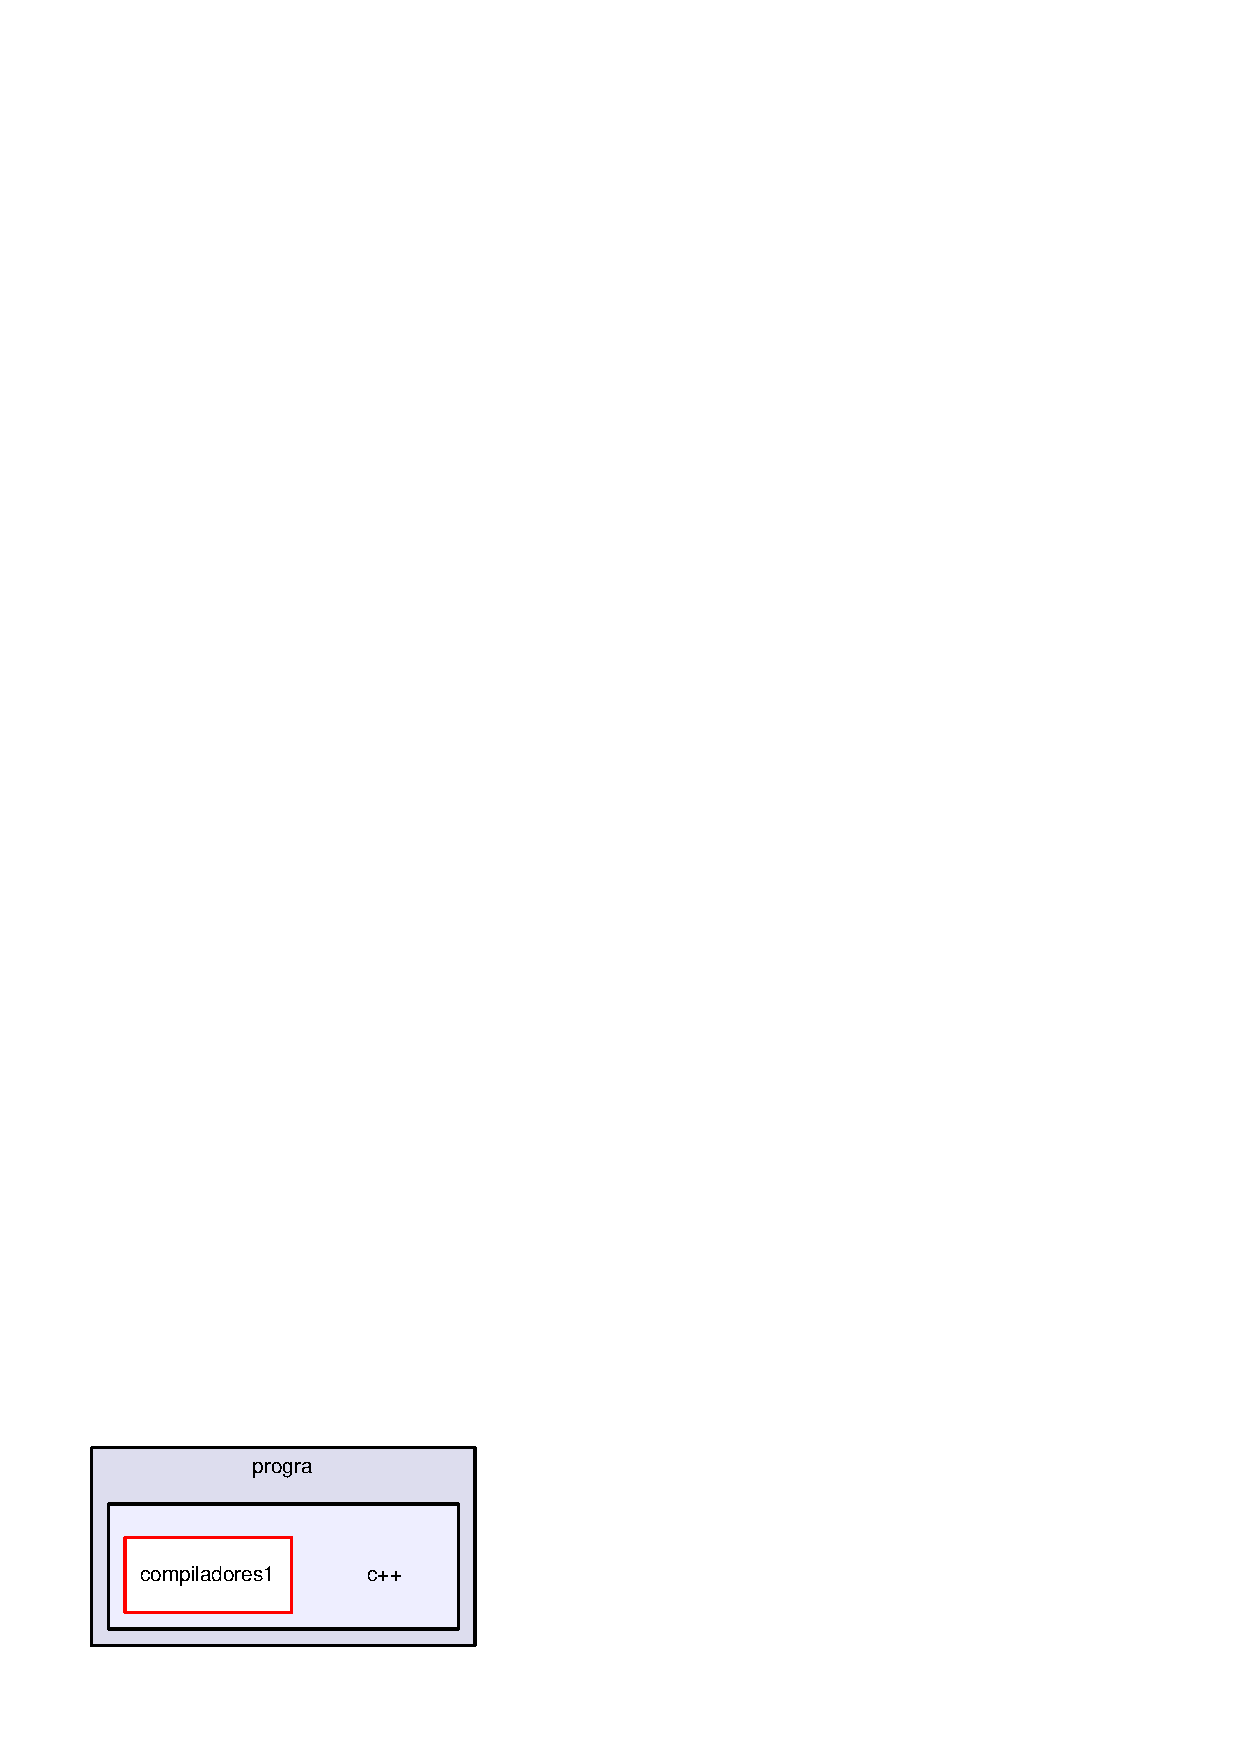
\includegraphics[width=118pt]{dir_000003_dep}
\end{center}
\end{figure}
\subsection*{Directories}
\begin{CompactItemize}
\item 
directory {\bf compiladores1}
\end{CompactItemize}

\section{/media/docs/progra/c++/compiladores1/ Directory Reference}
\label{dir_000004}\index{/media/docs/progra/c++/compiladores1/ Directory Reference@{/media/docs/progra/c++/compiladores1/ Directory Reference}}


\begin{figure}[H]
\begin{center}
\leavevmode
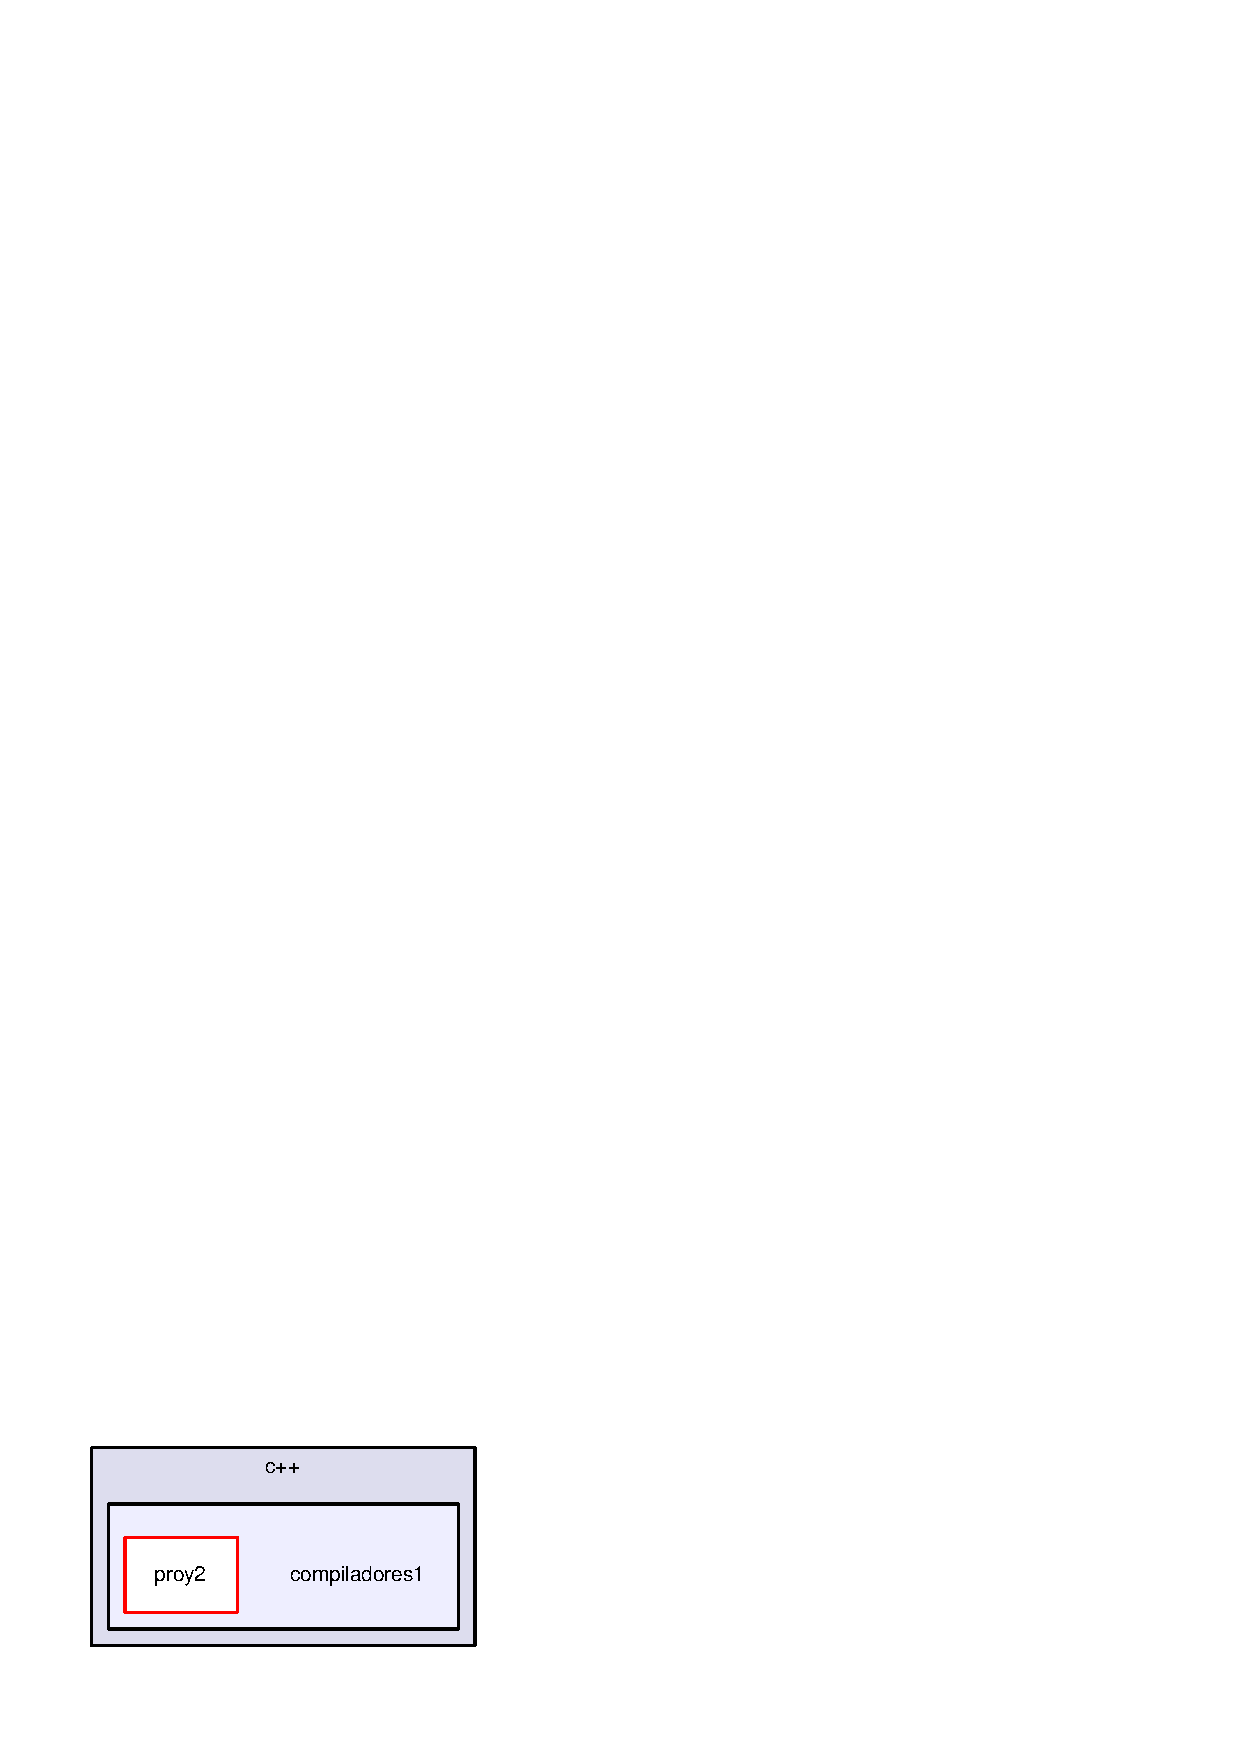
\includegraphics[width=118pt]{dir_000004_dep}
\end{center}
\end{figure}
\subsection*{Directories}
\begin{CompactItemize}
\item 
directory {\bf proy2}
\end{CompactItemize}

\section{/media/docs/ Directory Reference}
\label{dir_000001}\index{/media/docs/ Directory Reference@{/media/docs/ Directory Reference}}


\begin{figure}[H]
\begin{center}
\leavevmode
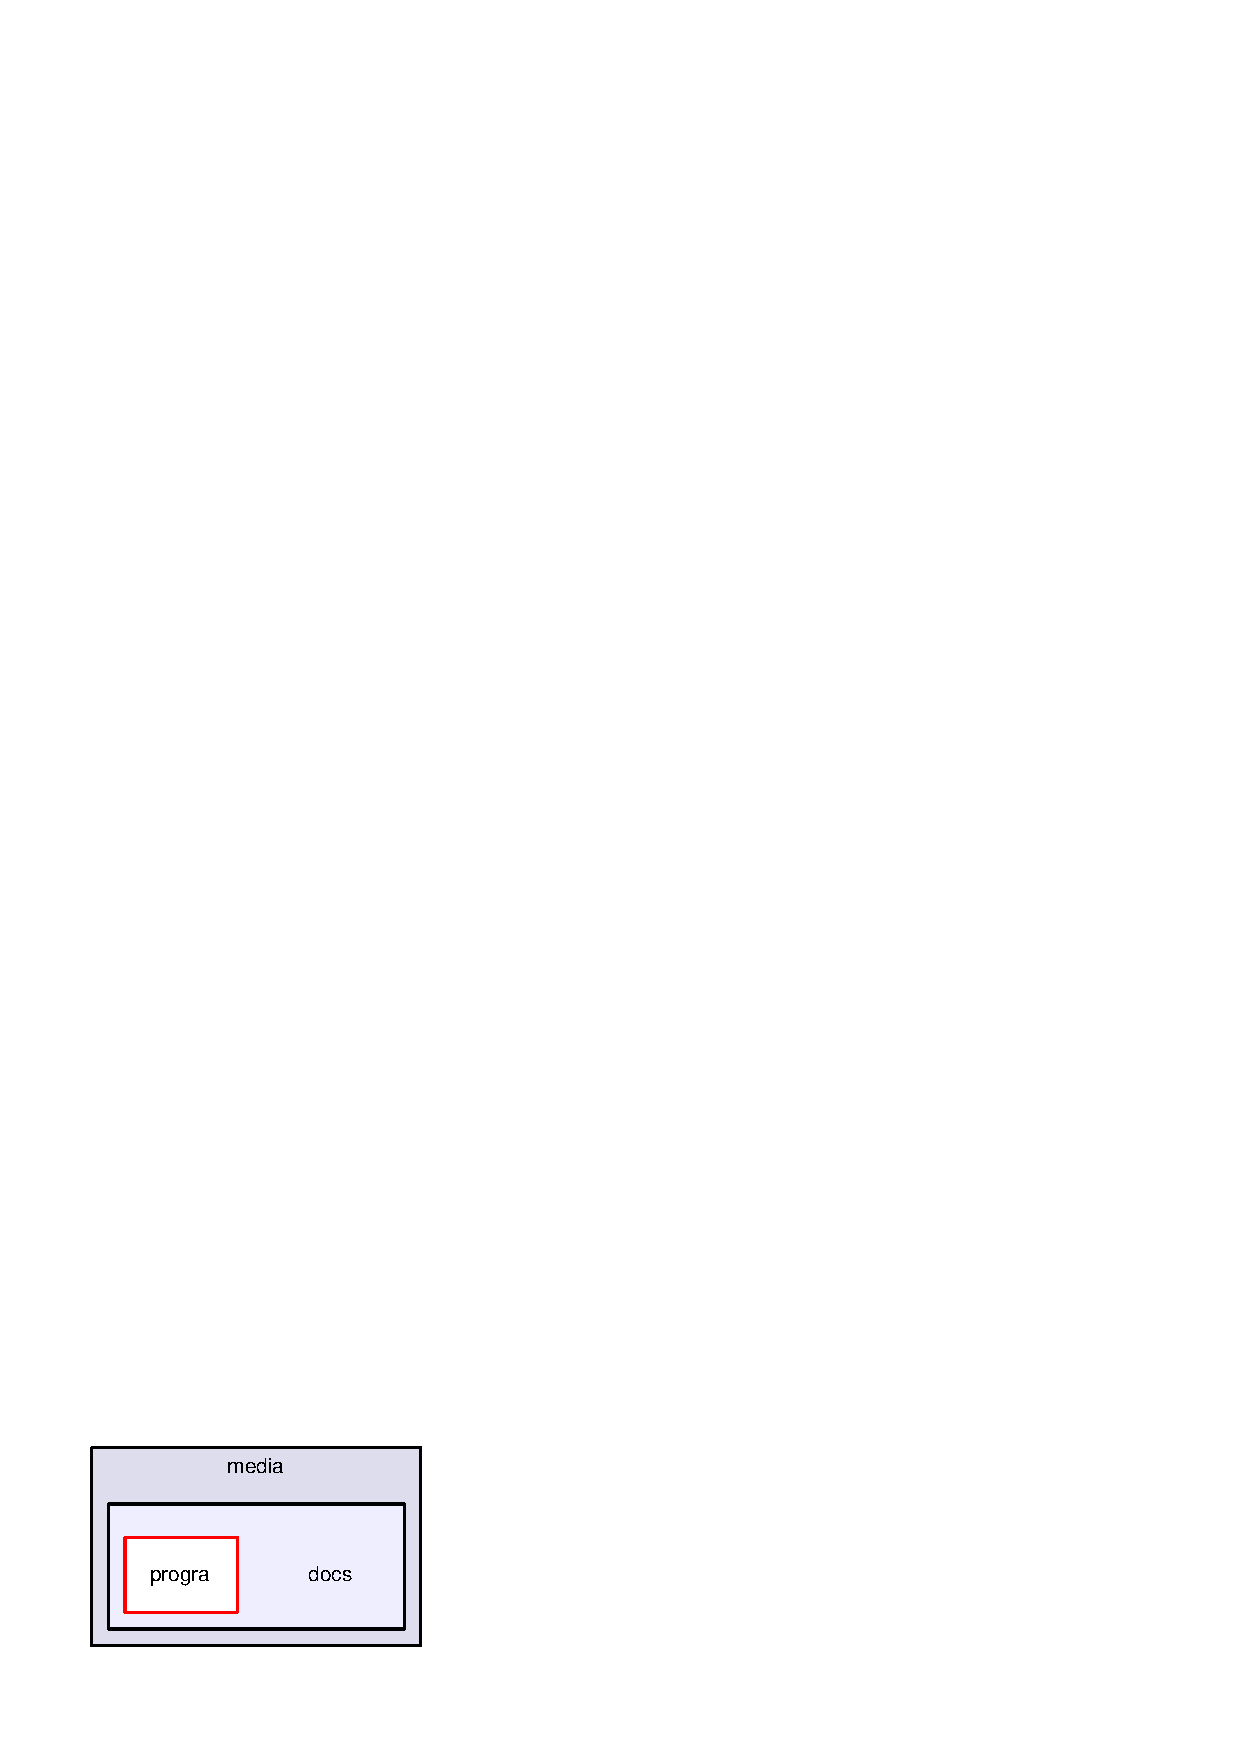
\includegraphics[width=105pt]{dir_000001_dep}
\end{center}
\end{figure}
\subsection*{Directories}
\begin{CompactItemize}
\item 
directory {\bf progra}
\end{CompactItemize}

\section{/media/docs/progra/c++/compiladores1/proy2/godzilla/ Directory Reference}
\label{dir_000006}\index{/media/docs/progra/c++/compiladores1/proy2/godzilla/ Directory Reference@{/media/docs/progra/c++/compiladores1/proy2/godzilla/ Directory Reference}}


\begin{figure}[H]
\begin{center}
\leavevmode
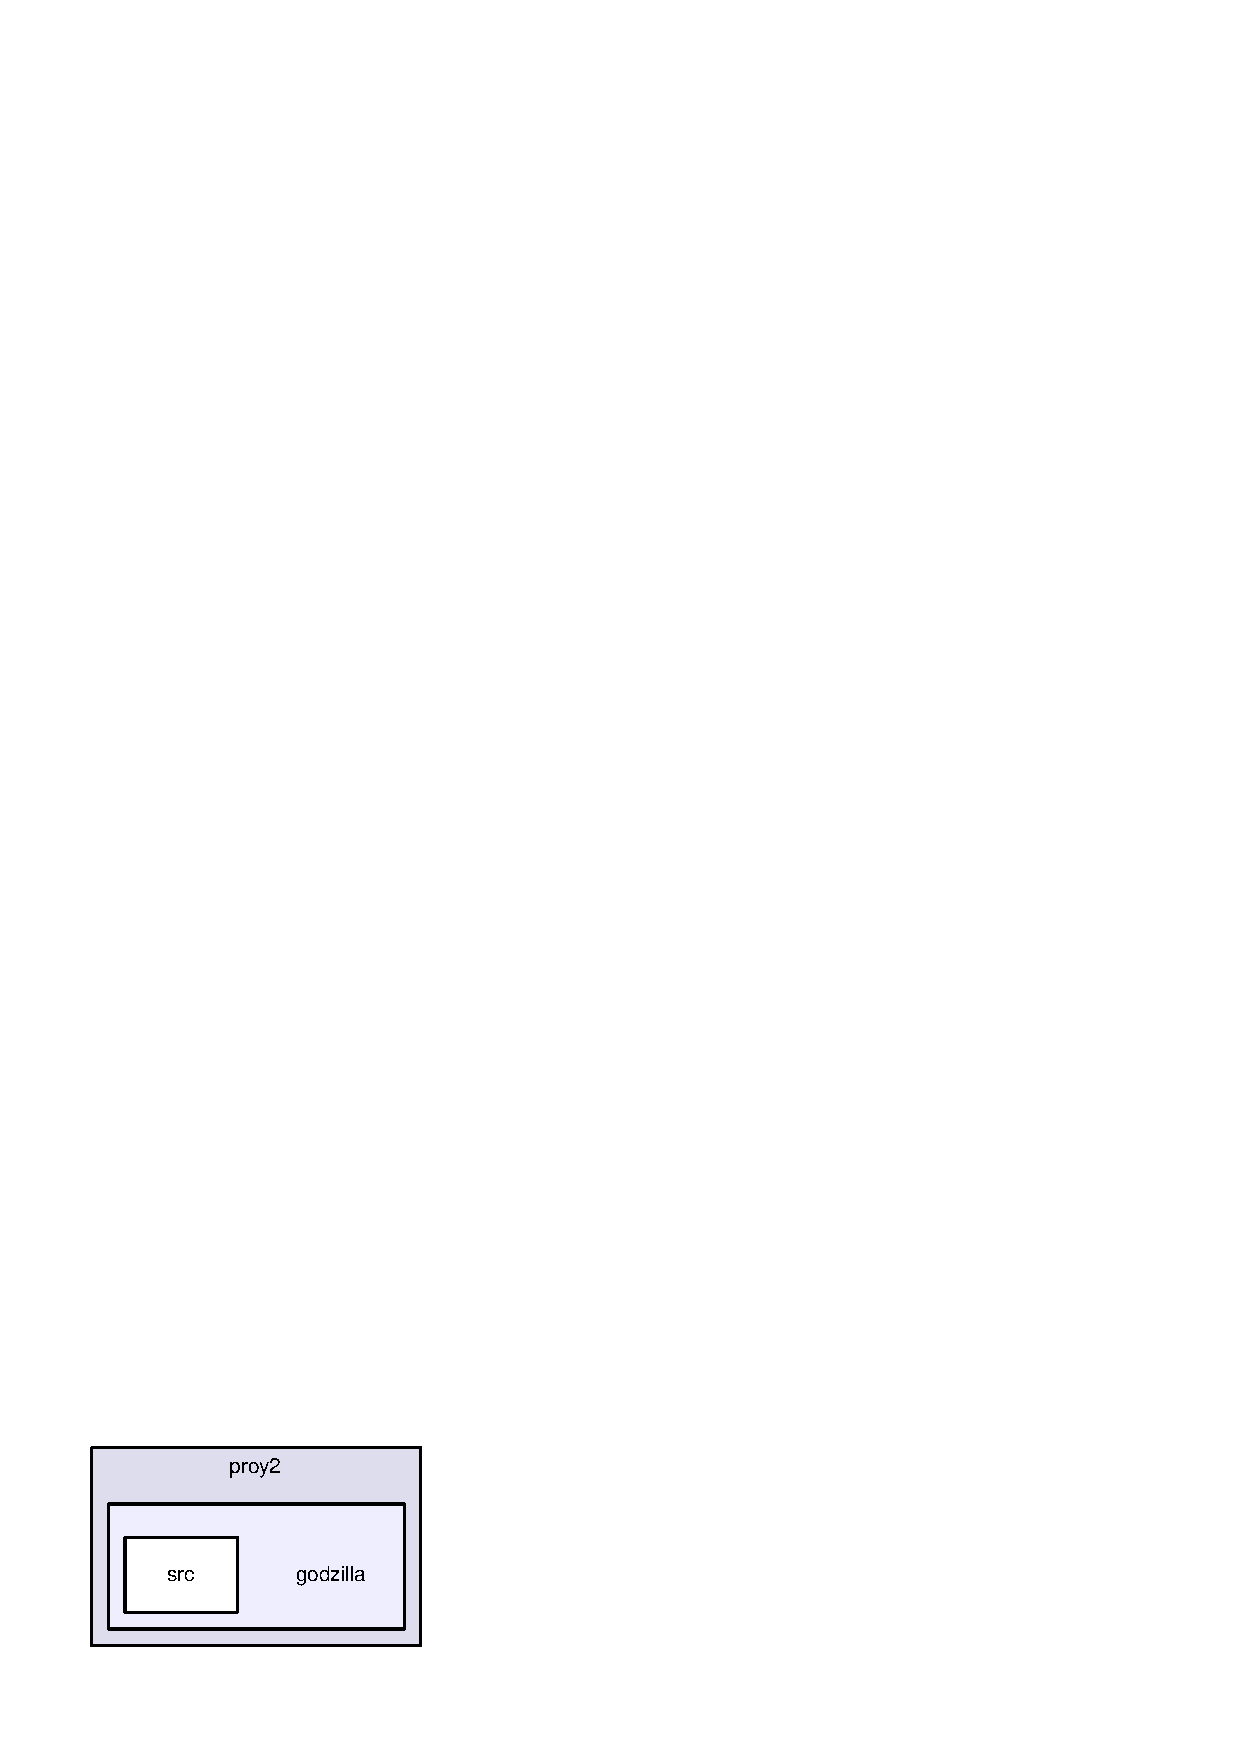
\includegraphics[width=105pt]{dir_000006_dep}
\end{center}
\end{figure}
\subsection*{Directories}
\begin{CompactItemize}
\item 
directory {\bf src}
\end{CompactItemize}

\section{/media/ Directory Reference}
\label{dir_000000}\index{/media/ Directory Reference@{/media/ Directory Reference}}


\begin{figure}[H]
\begin{center}
\leavevmode
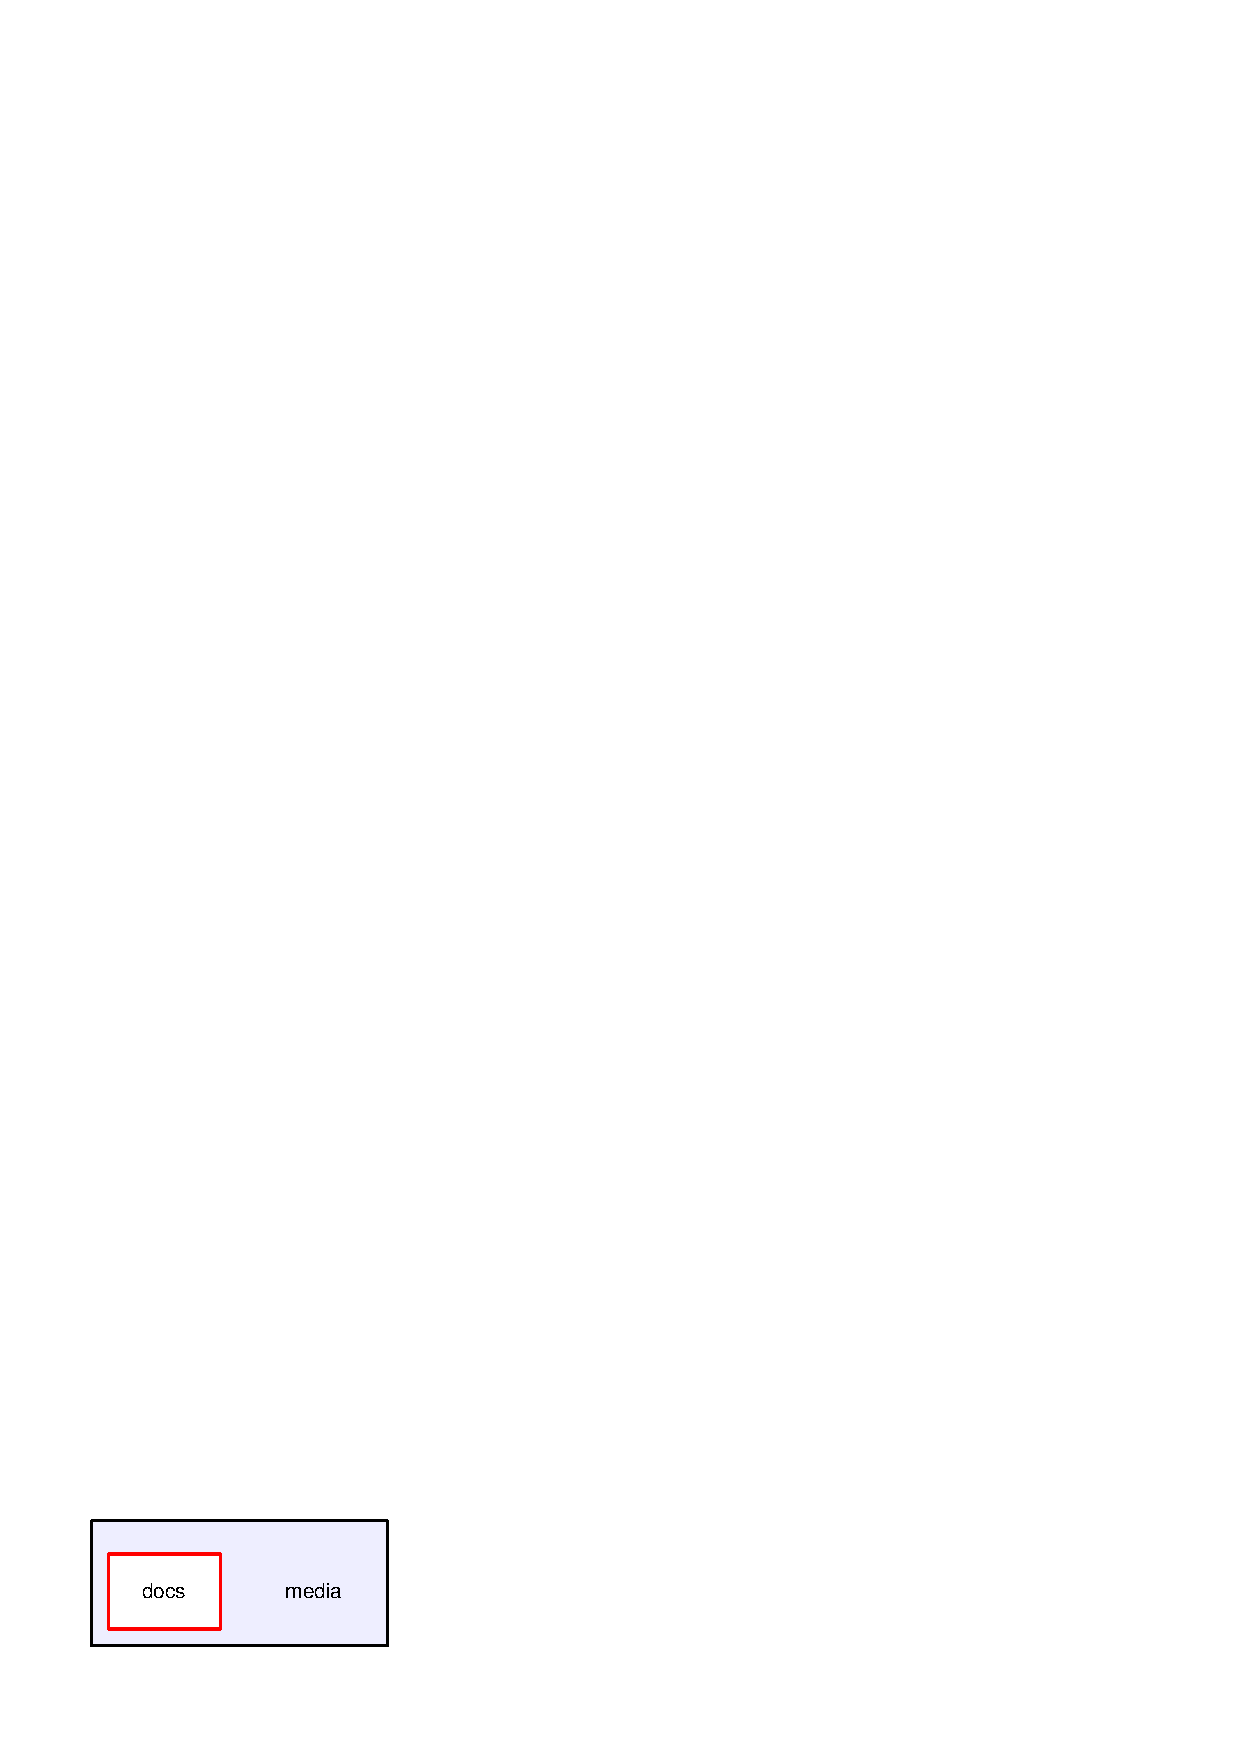
\includegraphics[width=97pt]{dir_000000_dep}
\end{center}
\end{figure}
\subsection*{Directories}
\begin{CompactItemize}
\item 
directory {\bf docs}
\end{CompactItemize}

\section{/media/docs/progra/ Directory Reference}
\label{dir_000002}\index{/media/docs/progra/ Directory Reference@{/media/docs/progra/ Directory Reference}}


\begin{figure}[H]
\begin{center}
\leavevmode
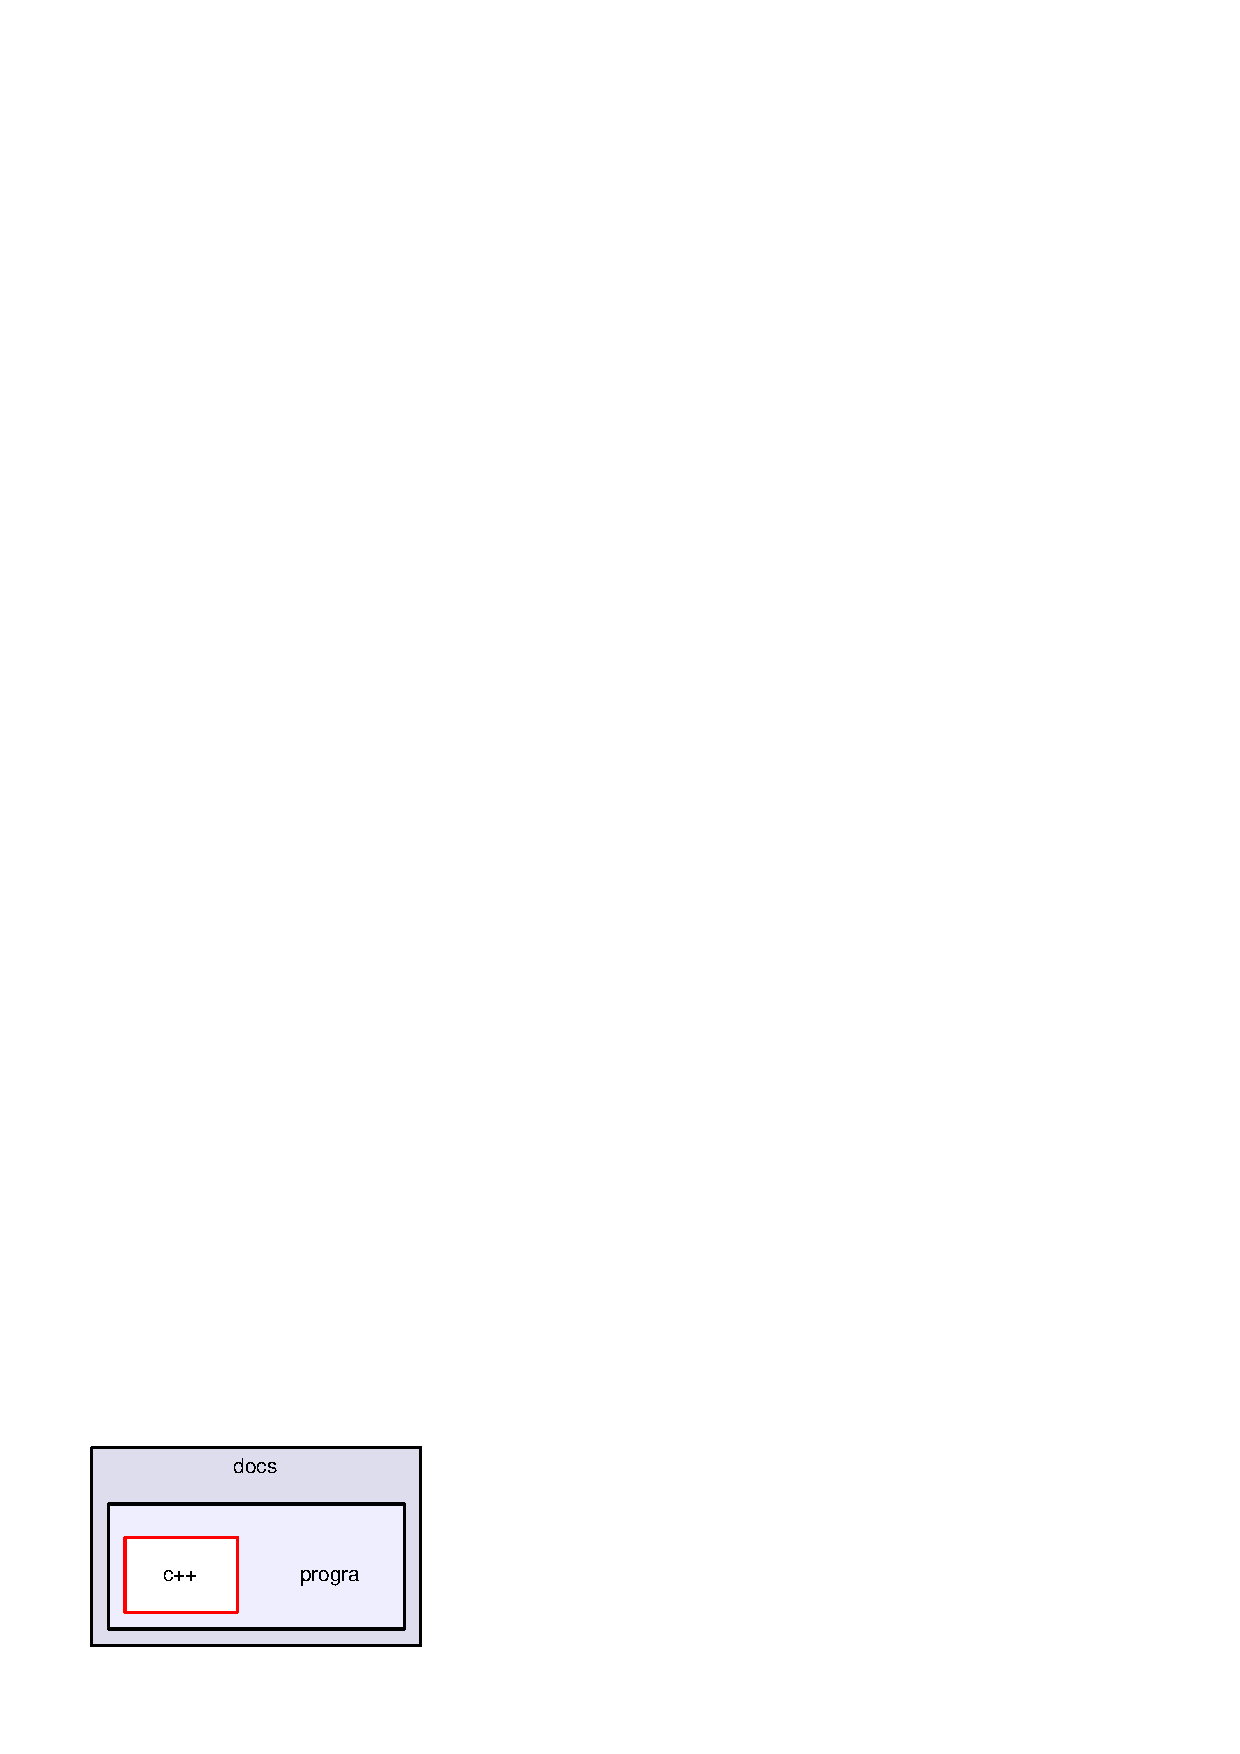
\includegraphics[width=105pt]{dir_000002_dep}
\end{center}
\end{figure}
\subsection*{Directories}
\begin{CompactItemize}
\item 
directory {\bf c++}
\end{CompactItemize}

\section{/media/docs/progra/c++/compiladores1/proy2/ Directory Reference}
\label{dir_000005}\index{/media/docs/progra/c++/compiladores1/proy2/ Directory Reference@{/media/docs/progra/c++/compiladores1/proy2/ Directory Reference}}


\begin{figure}[H]
\begin{center}
\leavevmode
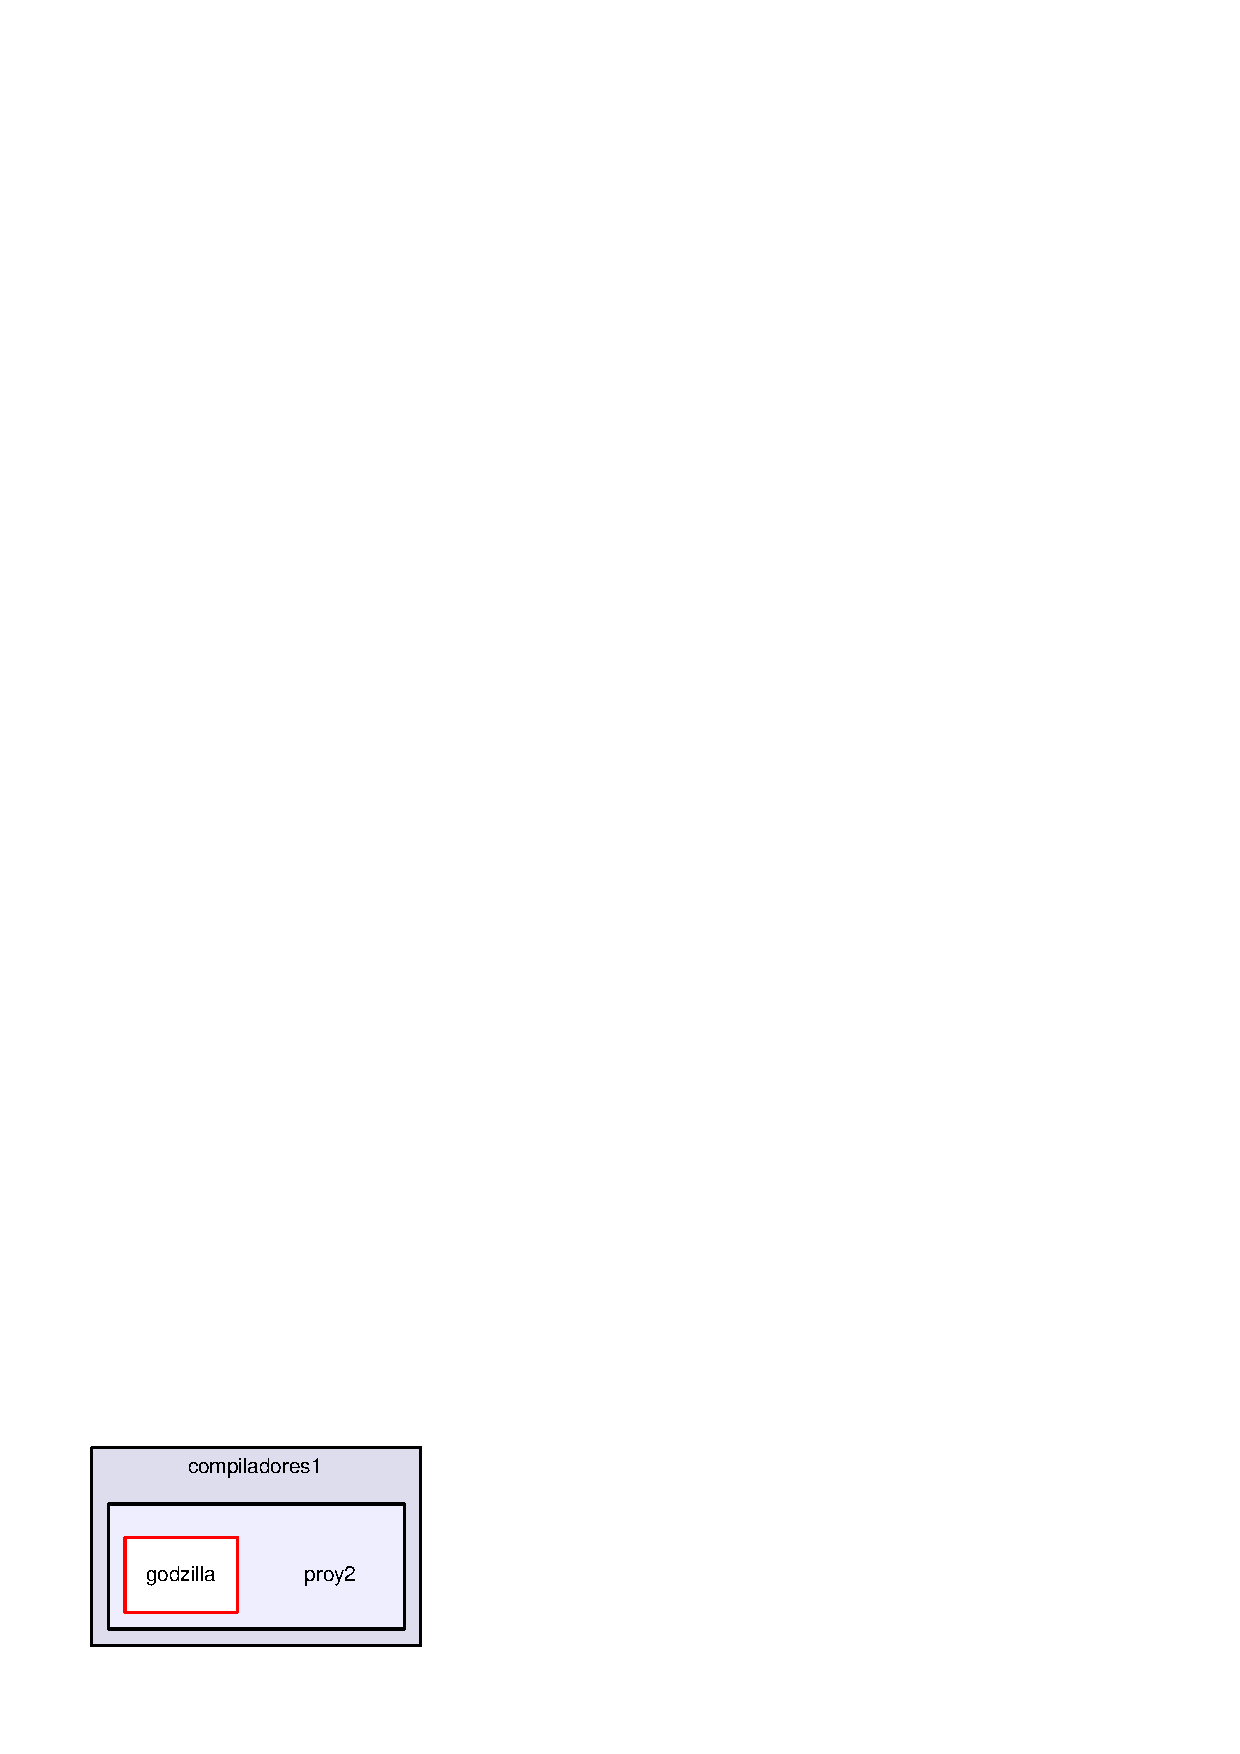
\includegraphics[width=105pt]{dir_000005_dep}
\end{center}
\end{figure}
\subsection*{Directories}
\begin{CompactItemize}
\item 
directory {\bf godzilla}
\end{CompactItemize}

\section{/media/docs/progra/c++/compiladores1/proy2/godzilla/src/ Directory Reference}
\label{dir_000007}\index{/media/docs/progra/c++/compiladores1/proy2/godzilla/src/ Directory Reference@{/media/docs/progra/c++/compiladores1/proy2/godzilla/src/ Directory Reference}}


\begin{figure}[H]
\begin{center}
\leavevmode
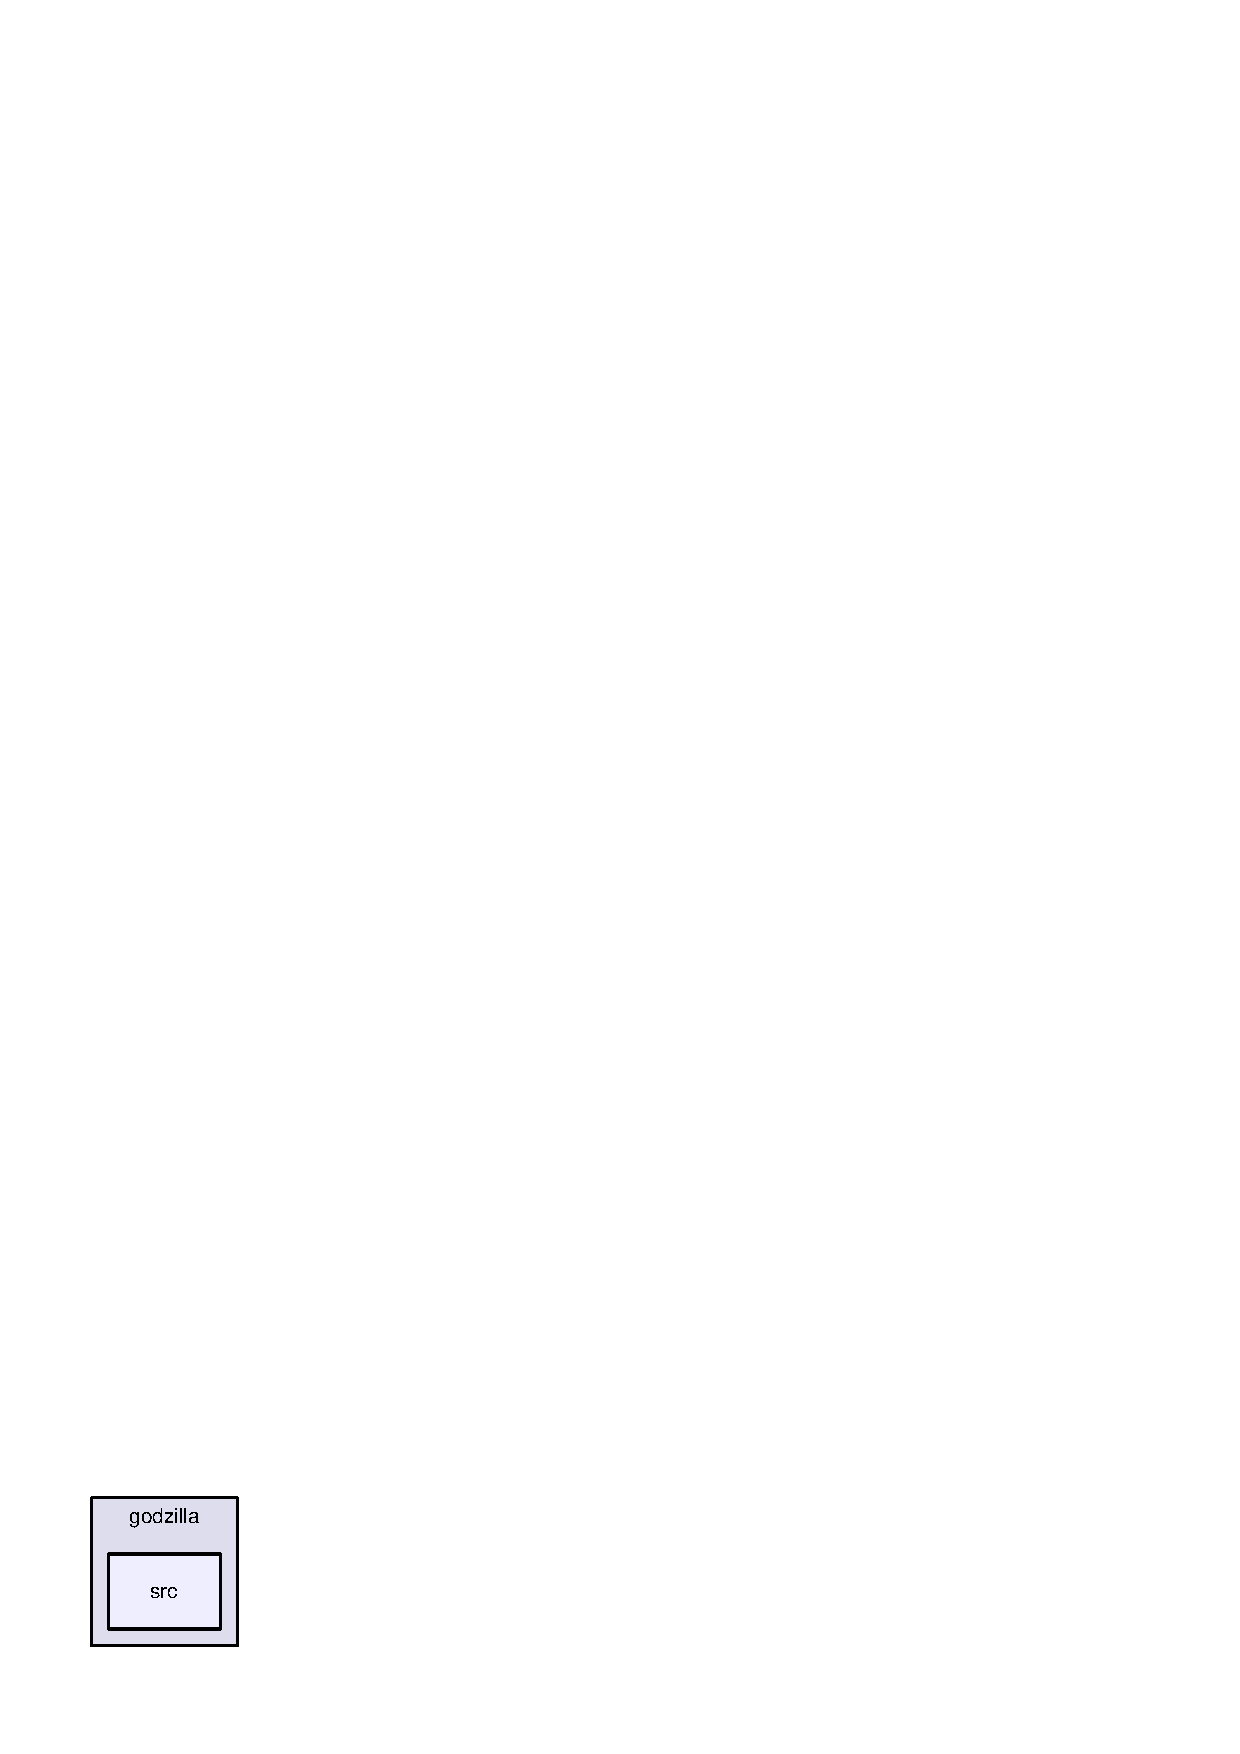
\includegraphics[width=61pt]{dir_000007_dep}
\end{center}
\end{figure}
\subsection*{Archivos}
\begin{CompactItemize}
\item 
archivo {\bf ast.c}
\begin{CompactList}\small\item\em Implementacion del arbol de sintaxis abstracta. \item\end{CompactList}

\item 
archivo {\bf ast.h}
\begin{CompactList}\small\item\em Definiciones y estructura del arbol de sintaxis abstracta. \item\end{CompactList}

\item 
archivo {\bf browser.cpp}
\begin{CompactList}\small\item\em Implementacion de la clase browser\-Dock. \item\end{CompactList}

\item 
archivo {\bf browser.h}
\begin{CompactList}\small\item\em Definiciones de la clase browser\-Dock. \item\end{CompactList}

\item 
archivo {\bf colaerr.c}
\begin{CompactList}\small\item\em Implementacion de la cola almacenadora de errores . \item\end{CompactList}

\item 
archivo {\bf colaerr.h}
\begin{CompactList}\small\item\em Definiciones de la cola almacenadora de errores . \item\end{CompactList}

\item 
archivo {\bf constantes.h}
\begin{CompactList}\small\item\em Constantes utilizadas por el arbol de sintaxis abstracta. \item\end{CompactList}

\item 
archivo {\bf godzilla.cpp}
\begin{CompactList}\small\item\em Implementacion de la Widged principal del GUI. \item\end{CompactList}

\item 
archivo {\bf godzilla.h}
\begin{CompactList}\small\item\em defiinicion de la Widged principal del GUI. \item\end{CompactList}

\item 
archivo {\bf main.cpp}
\begin{CompactList}\small\item\em Punto de entrada del programa. \item\end{CompactList}

\item 
archivo {\bf parserheader.h}
\begin{CompactList}\small\item\em interfaz entre el GUI y el parser. \item\end{CompactList}

\item 
archivo {\bf symtab.c}
\begin{CompactList}\small\item\em Implementacion de la tabla de simbolos.Incluye la implementacion de rutinas de insercion, busqueda y eliminacion. \item\end{CompactList}

\item 
archivo {\bf symtab.h}
\begin{CompactList}\small\item\em Estructuras de la tabla de simbolos.Incluyendo rutinas de insercion, busqueda y eliminacion. \item\end{CompactList}

\end{CompactItemize}

\chapter{godzilla Documentaci\'{o}n de clases}
\section{Referencia de la Estructura asignacion}
\label{structasignacion}\index{asignacion@{asignacion}}
Clase de almacenamiento de una asignacion en el AST.  


{\tt \#include $<$ast.h$>$}

Diagrama de colaboraci\'{o}n para asignacion:\begin{figure}[H]
\begin{center}
\leavevmode
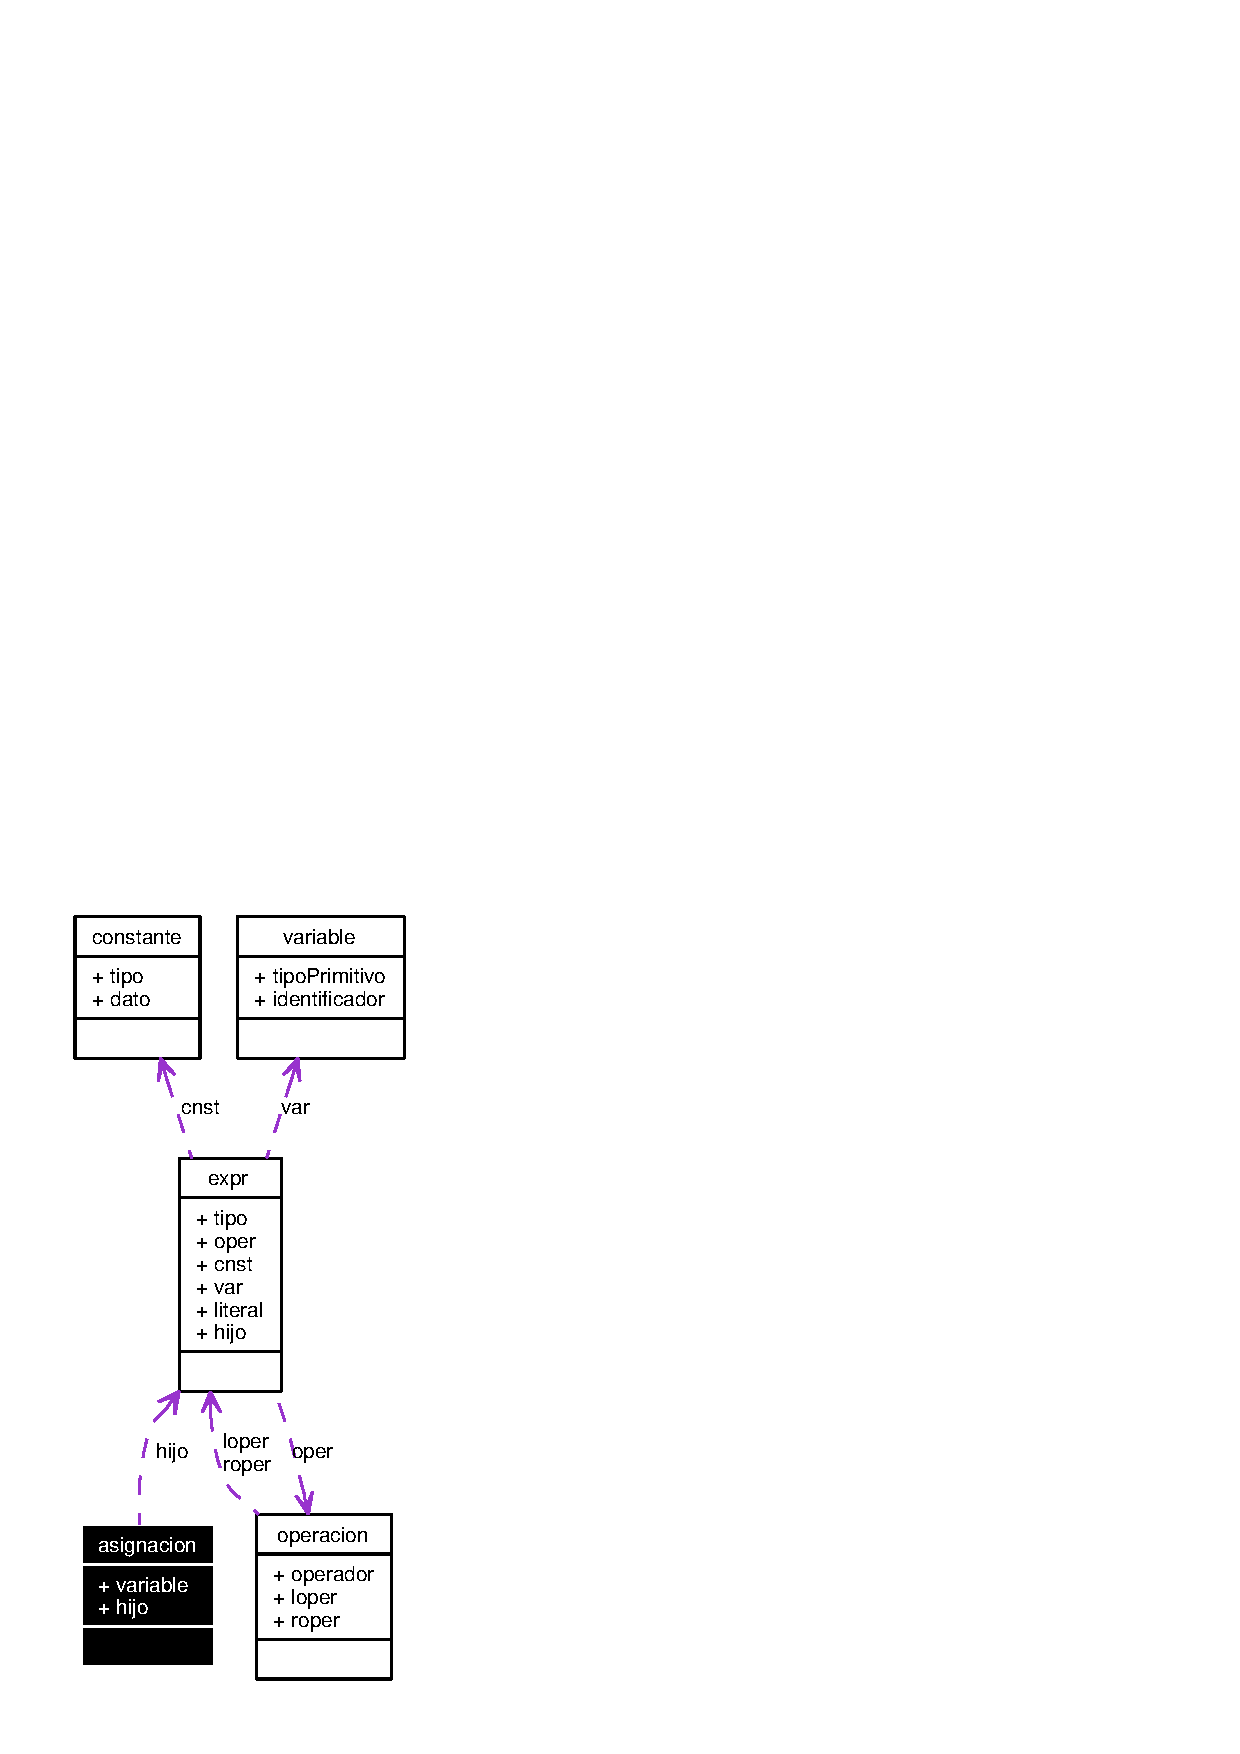
\includegraphics[width=97pt]{structasignacion__coll__graph}
\end{center}
\end{figure}
\subsection*{Atributos p\'{u}blicos}
\begin{CompactItemize}
\item 
char $\ast$ {\bf variable}
\begin{CompactList}\small\item\em Identificador de variable a asignar. \item\end{CompactList}\item 
{\bf expr} $\ast$ {\bf hijo}
\begin{CompactList}\small\item\em Expresion a evaluar para asignar valor. \item\end{CompactList}\end{CompactItemize}


\subsection{Descripci\'{o}n detallada}
Clase de almacenamiento de una asignacion en el AST. 



Definici\'{o}n en la l\'{\i}nea 216 del archivo ast.h.

\subsection{Documentaci\'{o}n de los datos miembro}
\index{asignacion@{asignacion}!hijo@{hijo}}
\index{hijo@{hijo}!asignacion@{asignacion}}
\subsubsection{\setlength{\rightskip}{0pt plus 5cm}{\bf expr}$\ast$ {\bf asignacion::hijo}}\label{structasignacion_o1}


Expresion a evaluar para asignar valor. 



Definici\'{o}n en la l\'{\i}nea 218 del archivo ast.h.

Referenciado por borrar\-Asignacion(), evaluar\-Asignacion(), y insertar\-Asignacion().\index{asignacion@{asignacion}!variable@{variable}}
\index{variable@{variable}!asignacion@{asignacion}}
\subsubsection{\setlength{\rightskip}{0pt plus 5cm}char$\ast$ {\bf asignacion::variable}}\label{structasignacion_o0}


Identificador de variable a asignar. 



Definici\'{o}n en la l\'{\i}nea 217 del archivo ast.h.

Referenciado por borrar\-Asignacion(), evaluar\-Asignacion(), y insertar\-Asignacion().

La documentaci\'{o}n para esta estructura fu\'{e} generada a partir del siguiente archivo:\begin{CompactItemize}
\item 
/media/docs/progra/c++/compiladores1/proy2/godzilla/src/{\bf ast.h}\end{CompactItemize}

\section{Referencia de la Estructura ast}
\label{structast}\index{ast@{ast}}
Estructura del arbol abstracto de sintaxis (AST), basico para poder evaluar construcciones iterativas del lenguaje.  


{\tt \#include $<$ast.h$>$}

Diagrama de colaboraci\'{o}n para ast:\begin{figure}[H]
\begin{center}
\leavevmode
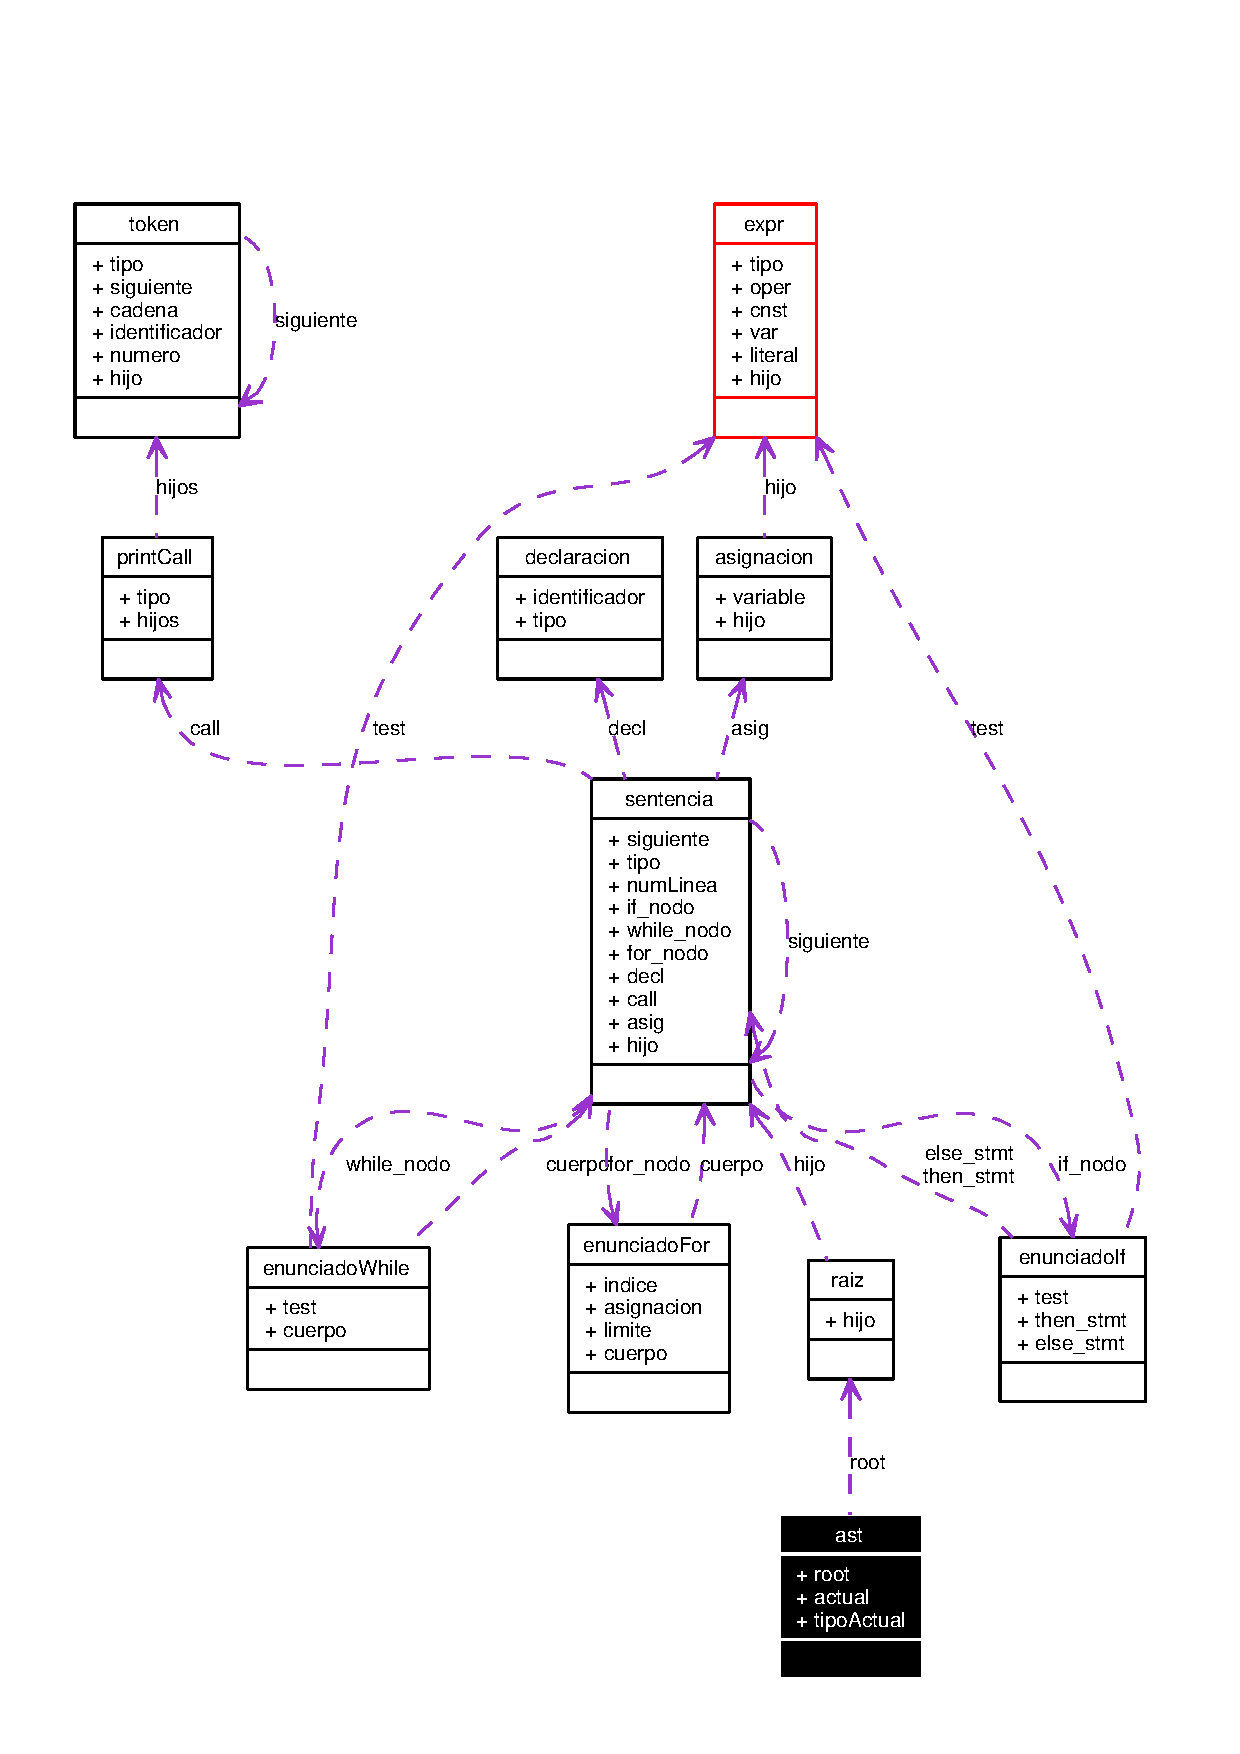
\includegraphics[width=290pt]{structast__coll__graph}
\end{center}
\end{figure}
\subsection*{Atributos p\'{u}blicos}
\begin{CompactItemize}
\item 
{\bf raiz} $\ast$ {\bf root}
\begin{CompactList}\small\item\em apuntador a raiz \item\end{CompactList}\item 
void $\ast$ {\bf actual}
\begin{CompactList}\small\item\em puntero auzliiar \item\end{CompactList}\item 
int {\bf tipo\-Actual}
\begin{CompactList}\small\item\em tipo del nodo actual \item\end{CompactList}\end{CompactItemize}


\subsection{Descripci\'{o}n detallada}
Estructura del arbol abstracto de sintaxis (AST), basico para poder evaluar construcciones iterativas del lenguaje. 



Definici\'{o}n en la l\'{\i}nea 268 del archivo ast.h.

\subsection{Documentaci\'{o}n de los datos miembro}
\index{ast@{ast}!actual@{actual}}
\index{actual@{actual}!ast@{ast}}
\subsubsection{\setlength{\rightskip}{0pt plus 5cm}void$\ast$ {\bf ast::actual}}\label{structast_o1}


puntero auzliiar 



Definici\'{o}n en la l\'{\i}nea 270 del archivo ast.h.

Referenciado por borrar\-Arbol(), y crear\-Raiz().\index{ast@{ast}!root@{root}}
\index{root@{root}!ast@{ast}}
\subsubsection{\setlength{\rightskip}{0pt plus 5cm}{\bf raiz}$\ast$ {\bf ast::root}}\label{structast_o0}


apuntador a raiz 



Definici\'{o}n en la l\'{\i}nea 269 del archivo ast.h.

Referenciado por borrar\-Arbol(), crear\-Raiz(), y recorrer\-Arbol().\index{ast@{ast}!tipoActual@{tipoActual}}
\index{tipoActual@{tipoActual}!ast@{ast}}
\subsubsection{\setlength{\rightskip}{0pt plus 5cm}int {\bf ast::tipo\-Actual}}\label{structast_o2}


tipo del nodo actual 



Definici\'{o}n en la l\'{\i}nea 271 del archivo ast.h.

Referenciado por borrar\-Arbol(), y crear\-Raiz().

La documentaci\'{o}n para esta estructura fu\'{e} generada a partir del siguiente archivo:\begin{CompactItemize}
\item 
/media/docs/progra/c++/compiladores1/proy2/godzilla/src/{\bf ast.h}\end{CompactItemize}

\section{Referencia de la Clase Browser\-Dock}
\label{classBrowserDock}\index{BrowserDock@{BrowserDock}}
Dock\-Window del browser empotrable en la ventana principal, heredando de QDock\-Window.  


{\tt \#include $<$browser.h$>$}

\subsection*{M\'{e}todos p\'{u}blicos}
\begin{CompactItemize}
\item 
{\bf Browser\-Dock} (QWidget $\ast$parent, const char $\ast$name=0, WFlags f=0)
\begin{CompactList}\small\item\em Constructor, llama al constructor padre con los mismos parametros. \item\end{CompactList}\item 
{\bf Browser\-Dock} (Place p, QWidget $\ast$parent, const char $\ast$name, WFlags f)
\begin{CompactList}\small\item\em Constructor, llama al constructor padre con los mismos parametros. \item\end{CompactList}\item 
{\bf $\sim$Browser\-Dock} ()
\item 
void {\bf set\-Source} (QString filename)
\begin{CompactList}\small\item\em Abre el archivo dado en el browser. \item\end{CompactList}\item 
void {\bf set\-Label} (QString label)
\begin{CompactList}\small\item\em Asigna titulo de ventana. \item\end{CompactList}\item 
void {\bf orientacion} (Orientation o)
\begin{CompactList}\small\item\em establece orientacion para el browserdock \item\end{CompactList}\end{CompactItemize}
\subsection*{Atributos privados}
\begin{CompactItemize}
\item 
QText\-Browser $\ast$ {\bf b}
\end{CompactItemize}


\subsection{Descripci\'{o}n detallada}
Dock\-Window del browser empotrable en la ventana principal, heredando de QDock\-Window. 



Definici\'{o}n en la l\'{\i}nea 13 del archivo browser.h.

\subsection{Documentaci\'{o}n del constructor y destructor}
\index{BrowserDock@{Browser\-Dock}!BrowserDock@{BrowserDock}}
\index{BrowserDock@{BrowserDock}!BrowserDock@{Browser\-Dock}}
\subsubsection{\setlength{\rightskip}{0pt plus 5cm}Browser\-Dock::Browser\-Dock (QWidget $\ast$ {\em parent}, const char $\ast$ {\em name} = {\tt 0}, WFlags {\em f} = {\tt 0})}\label{classBrowserDock_a0}


Constructor, llama al constructor padre con los mismos parametros. 



Definici\'{o}n en la l\'{\i}nea 11 del archivo browser.cpp.

Hace referencia a b.\index{BrowserDock@{Browser\-Dock}!BrowserDock@{BrowserDock}}
\index{BrowserDock@{BrowserDock}!BrowserDock@{Browser\-Dock}}
\subsubsection{\setlength{\rightskip}{0pt plus 5cm}Browser\-Dock::Browser\-Dock (Place {\em p}, QWidget $\ast$ {\em parent}, const char $\ast$ {\em name}, WFlags {\em f})}\label{classBrowserDock_a1}


Constructor, llama al constructor padre con los mismos parametros. 



Definici\'{o}n en la l\'{\i}nea 23 del archivo browser.cpp.

Hace referencia a b.\index{BrowserDock@{Browser\-Dock}!~BrowserDock@{$\sim$BrowserDock}}
\index{~BrowserDock@{$\sim$BrowserDock}!BrowserDock@{Browser\-Dock}}
\subsubsection{\setlength{\rightskip}{0pt plus 5cm}Browser\-Dock::$\sim$Browser\-Dock ()}\label{classBrowserDock_a2}




Definici\'{o}n en la l\'{\i}nea 34 del archivo browser.cpp.

Hace referencia a b.

\subsection{Documentaci\'{o}n de las funciones miembro}
\index{BrowserDock@{Browser\-Dock}!orientacion@{orientacion}}
\index{orientacion@{orientacion}!BrowserDock@{Browser\-Dock}}
\subsubsection{\setlength{\rightskip}{0pt plus 5cm}void Browser\-Dock::orientacion (Orientation {\em o})}\label{classBrowserDock_a5}


establece orientacion para el browserdock 



Definici\'{o}n en la l\'{\i}nea 56 del archivo browser.cpp.\index{BrowserDock@{Browser\-Dock}!setLabel@{setLabel}}
\index{setLabel@{setLabel}!BrowserDock@{Browser\-Dock}}
\subsubsection{\setlength{\rightskip}{0pt plus 5cm}void Browser\-Dock::set\-Label (QString {\em label})}\label{classBrowserDock_a4}


Asigna titulo de ventana. 

\begin{Desc}
\item[Par\'{a}metros:]
\begin{description}
\item[{\em label}]cadena de nombre \end{description}
\end{Desc}


Definici\'{o}n en la l\'{\i}nea 52 del archivo browser.cpp.

Referenciado por God\-Zilla::God\-Zilla().\index{BrowserDock@{Browser\-Dock}!setSource@{setSource}}
\index{setSource@{setSource}!BrowserDock@{Browser\-Dock}}
\subsubsection{\setlength{\rightskip}{0pt plus 5cm}void Browser\-Dock::set\-Source (QString {\em file\-Name})}\label{classBrowserDock_a3}


Abre el archivo dado en el browser. 

\begin{Desc}
\item[Par\'{a}metros:]
\begin{description}
\item[{\em file\-Name}]nombre de archivo a mostrar en el Qtext\-Browser \end{description}
\end{Desc}


Definici\'{o}n en la l\'{\i}nea 39 del archivo browser.cpp.

Hace referencia a b.

Referenciado por God\-Zilla::leer\-Archivo\-Error(), God\-Zilla::leer\-Archivo\-Salida(), God\-Zilla::leer\-Archivo\-Tabla\-Simbolos(), y God\-Zilla::parse\-Input().

\subsection{Documentaci\'{o}n de los datos miembro}
\index{BrowserDock@{Browser\-Dock}!b@{b}}
\index{b@{b}!BrowserDock@{Browser\-Dock}}
\subsubsection{\setlength{\rightskip}{0pt plus 5cm}QText\-Browser$\ast$ {\bf Browser\-Dock::b}\hspace{0.3cm}{\tt  [private]}}\label{classBrowserDock_r0}




Definici\'{o}n en la l\'{\i}nea 22 del archivo browser.h.

Referenciado por Browser\-Dock(), set\-Source(), y $\sim$Browser\-Dock().

La documentaci\'{o}n para esta clase fu\'{e} generada a partir de los siguientes archivos:\begin{CompactItemize}
\item 
/media/docs/progra/c++/compiladores1/proy2/godzilla/src/{\bf browser.h}\item 
/media/docs/progra/c++/compiladores1/proy2/godzilla/src/{\bf browser.cpp}\end{CompactItemize}

\section{Referencia de la Estructura cola\-Err}
\label{structcolaErr}\index{colaErr@{colaErr}}
Cola de errores.  


{\tt \#include $<$colaerr.h$>$}

Diagrama de colaboraci\'{o}n para cola\-Err:\begin{figure}[H]
\begin{center}
\leavevmode
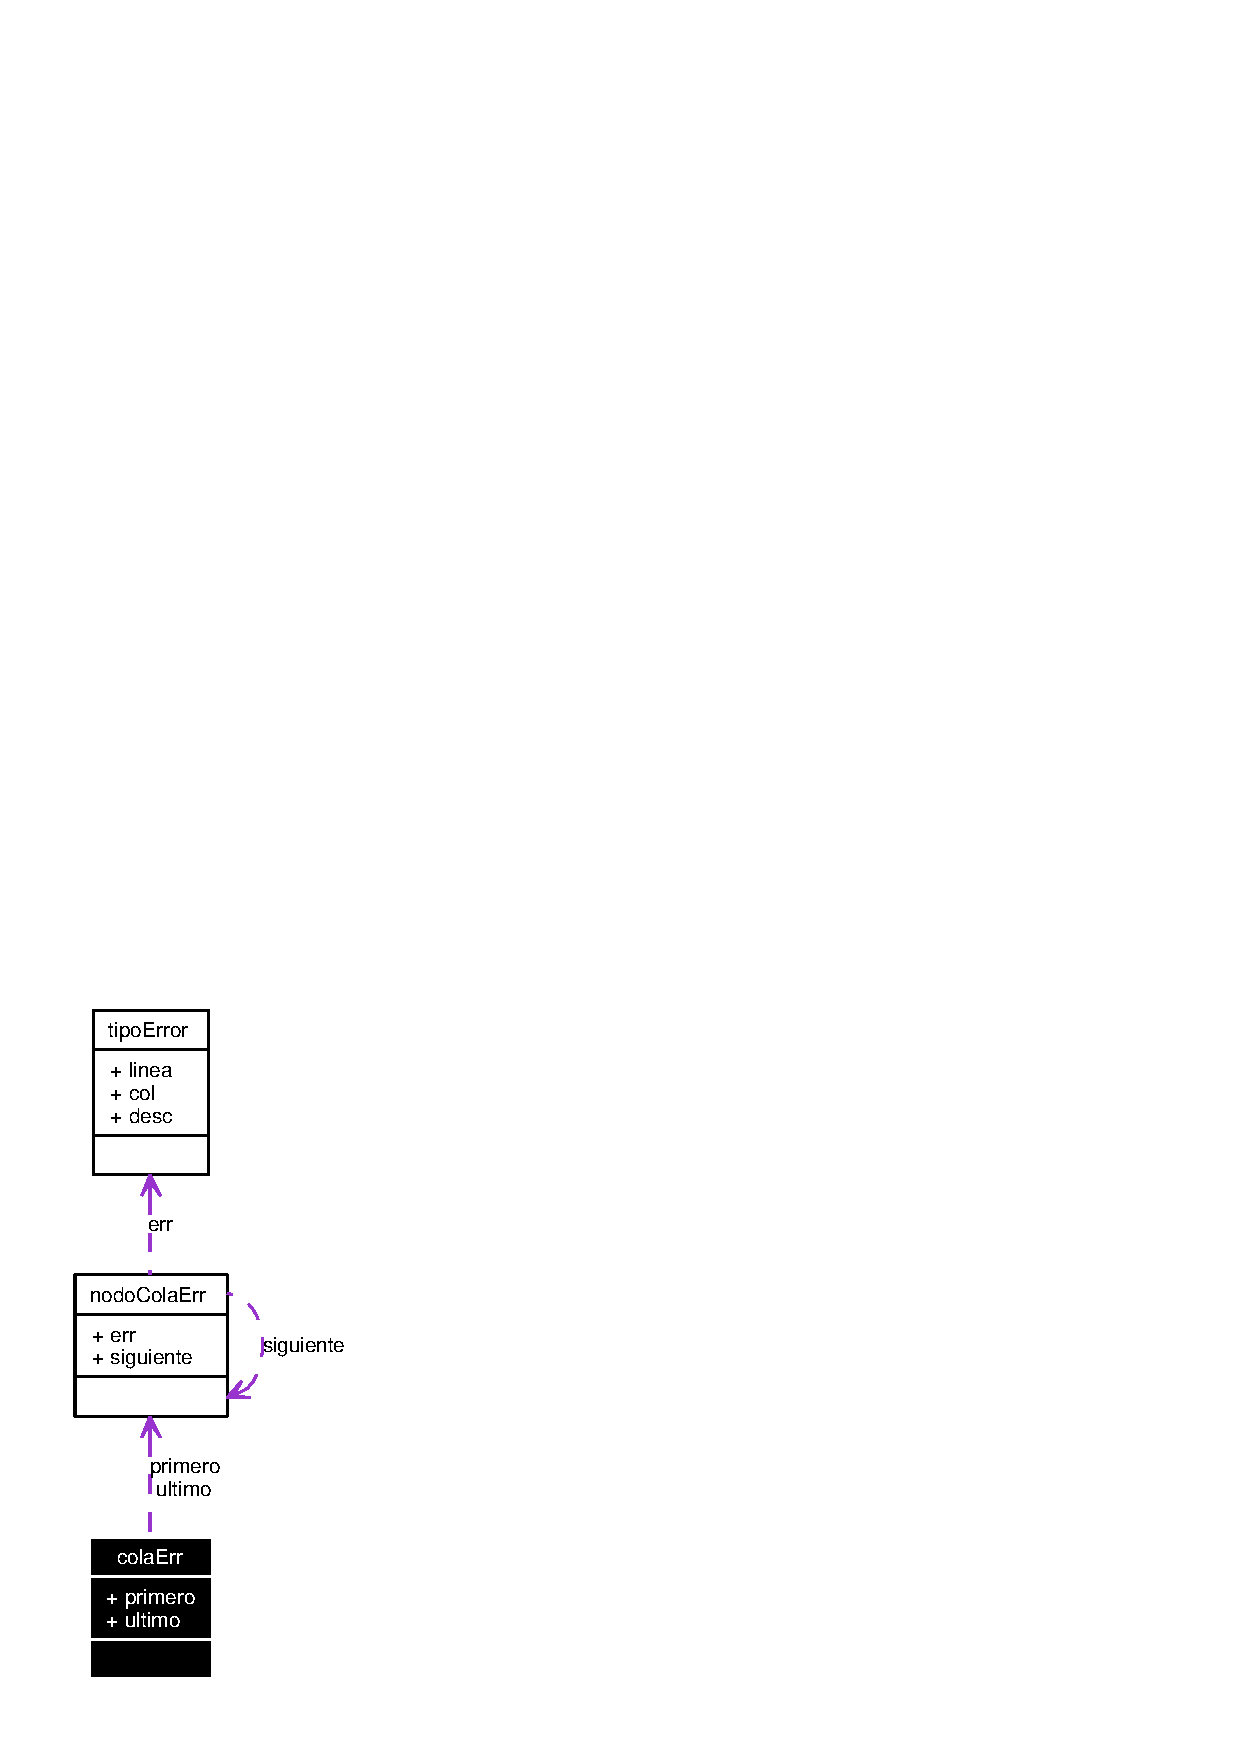
\includegraphics[width=83pt]{structcolaErr__coll__graph}
\end{center}
\end{figure}
\subsection*{Atributos p\'{u}blicos}
\begin{CompactItemize}
\item 
{\bf nodo\-Cola\-Err} $\ast$ {\bf primero}
\item 
{\bf nodo\-Cola\-Err} $\ast$ {\bf ultimo}
\end{CompactItemize}


\subsection{Descripci\'{o}n detallada}
Cola de errores. 



Definici\'{o}n en la l\'{\i}nea 39 del archivo colaerr.h.

\subsection{Documentaci\'{o}n de los datos miembro}
\index{colaErr@{cola\-Err}!primero@{primero}}
\index{primero@{primero}!colaErr@{cola\-Err}}
\subsubsection{\setlength{\rightskip}{0pt plus 5cm}{\bf nodo\-Cola\-Err}$\ast$ {\bf cola\-Err::primero}}\label{structcolaErr_o0}




Definici\'{o}n en la l\'{\i}nea 40 del archivo colaerr.h.

Referenciado por encolar\-Error(), escribir\-Error\-Log\-XML(), y sacar\-Error().\index{colaErr@{cola\-Err}!ultimo@{ultimo}}
\index{ultimo@{ultimo}!colaErr@{cola\-Err}}
\subsubsection{\setlength{\rightskip}{0pt plus 5cm}{\bf nodo\-Cola\-Err}$\ast$ {\bf cola\-Err::ultimo}}\label{structcolaErr_o1}




Definici\'{o}n en la l\'{\i}nea 41 del archivo colaerr.h.

Referenciado por encolar\-Error(), y sacar\-Error().

La documentaci\'{o}n para esta estructura fu\'{e} generada a partir del siguiente archivo:\begin{CompactItemize}
\item 
/media/docs/progra/c++/compiladores1/proy2/godzilla/src/{\bf colaerr.h}\end{CompactItemize}

\section{Referencia de la Estructura constante}
\label{structconstante}\index{constante@{constante}}
Clase de almacenamiento de constantes en el AST.  


{\tt \#include $<$ast.h$>$}

\subsection*{Atributos p\'{u}blicos}
\begin{CompactItemize}
\item 
int {\bf tipo}
\begin{CompactList}\small\item\em Tipo de constante. \item\end{CompactList}\item 
int {\bf dato}
\begin{CompactList}\small\item\em Valor. \item\end{CompactList}\end{CompactItemize}


\subsection{Descripci\'{o}n detallada}
Clase de almacenamiento de constantes en el AST. 



Definici\'{o}n en la l\'{\i}nea 174 del archivo ast.h.

\subsection{Documentaci\'{o}n de los datos miembro}
\index{constante@{constante}!dato@{dato}}
\index{dato@{dato}!constante@{constante}}
\subsubsection{\setlength{\rightskip}{0pt plus 5cm}int {\bf constante::dato}}\label{structconstante_o1}


Valor. 



Definici\'{o}n en la l\'{\i}nea 176 del archivo ast.h.

Referenciado por insertar\-Constante().\index{constante@{constante}!tipo@{tipo}}
\index{tipo@{tipo}!constante@{constante}}
\subsubsection{\setlength{\rightskip}{0pt plus 5cm}int {\bf constante::tipo}}\label{structconstante_o0}


Tipo de constante. 



Definici\'{o}n en la l\'{\i}nea 175 del archivo ast.h.

Referenciado por insertar\-Constante().

La documentaci\'{o}n para esta estructura fu\'{e} generada a partir del siguiente archivo:\begin{CompactItemize}
\item 
/media/docs/progra/c++/compiladores1/proy2/godzilla/src/{\bf ast.h}\end{CompactItemize}

\section{Referencia de la Estructura declaracion}
\label{structdeclaracion}\index{declaracion@{declaracion}}
Clase de almacenamiento de raiz de una declaracion en el AST.  


{\tt \#include $<$ast.h$>$}

\subsection*{Atributos p\'{u}blicos}
\begin{CompactItemize}
\item 
char $\ast$ {\bf identificador}
\begin{CompactList}\small\item\em Identificador de variable a declarar. \item\end{CompactList}\item 
int {\bf tipo}
\begin{CompactList}\small\item\em Tipo de dato de la variable. \item\end{CompactList}\end{CompactItemize}


\subsection{Descripci\'{o}n detallada}
Clase de almacenamiento de raiz de una declaracion en el AST. 



Definici\'{o}n en la l\'{\i}nea 253 del archivo ast.h.

\subsection{Documentaci\'{o}n de los datos miembro}
\index{declaracion@{declaracion}!identificador@{identificador}}
\index{identificador@{identificador}!declaracion@{declaracion}}
\subsubsection{\setlength{\rightskip}{0pt plus 5cm}char$\ast$ {\bf declaracion::identificador}}\label{structdeclaracion_o0}


Identificador de variable a declarar. 



Definici\'{o}n en la l\'{\i}nea 254 del archivo ast.h.

Referenciado por borrar\-Declaracion(), evaluar\-Declaracion(), y insertar\-Declaracion().\index{declaracion@{declaracion}!tipo@{tipo}}
\index{tipo@{tipo}!declaracion@{declaracion}}
\subsubsection{\setlength{\rightskip}{0pt plus 5cm}int {\bf declaracion::tipo}}\label{structdeclaracion_o1}


Tipo de dato de la variable. 



Definici\'{o}n en la l\'{\i}nea 255 del archivo ast.h.

Referenciado por evaluar\-Declaracion(), y insertar\-Declaracion().

La documentaci\'{o}n para esta estructura fu\'{e} generada a partir del siguiente archivo:\begin{CompactItemize}
\item 
/media/docs/progra/c++/compiladores1/proy2/godzilla/src/{\bf ast.h}\end{CompactItemize}

\section{Referencia de la Estructura enunciado\-For}
\label{structenunciadoFor}\index{enunciadoFor@{enunciadoFor}}
Clase de almacenamiento de enunciados for en el AST.  


{\tt \#include $<$ast.h$>$}

Diagrama de colaboraci\'{o}n para enunciado\-For:\begin{figure}[H]
\begin{center}
\leavevmode
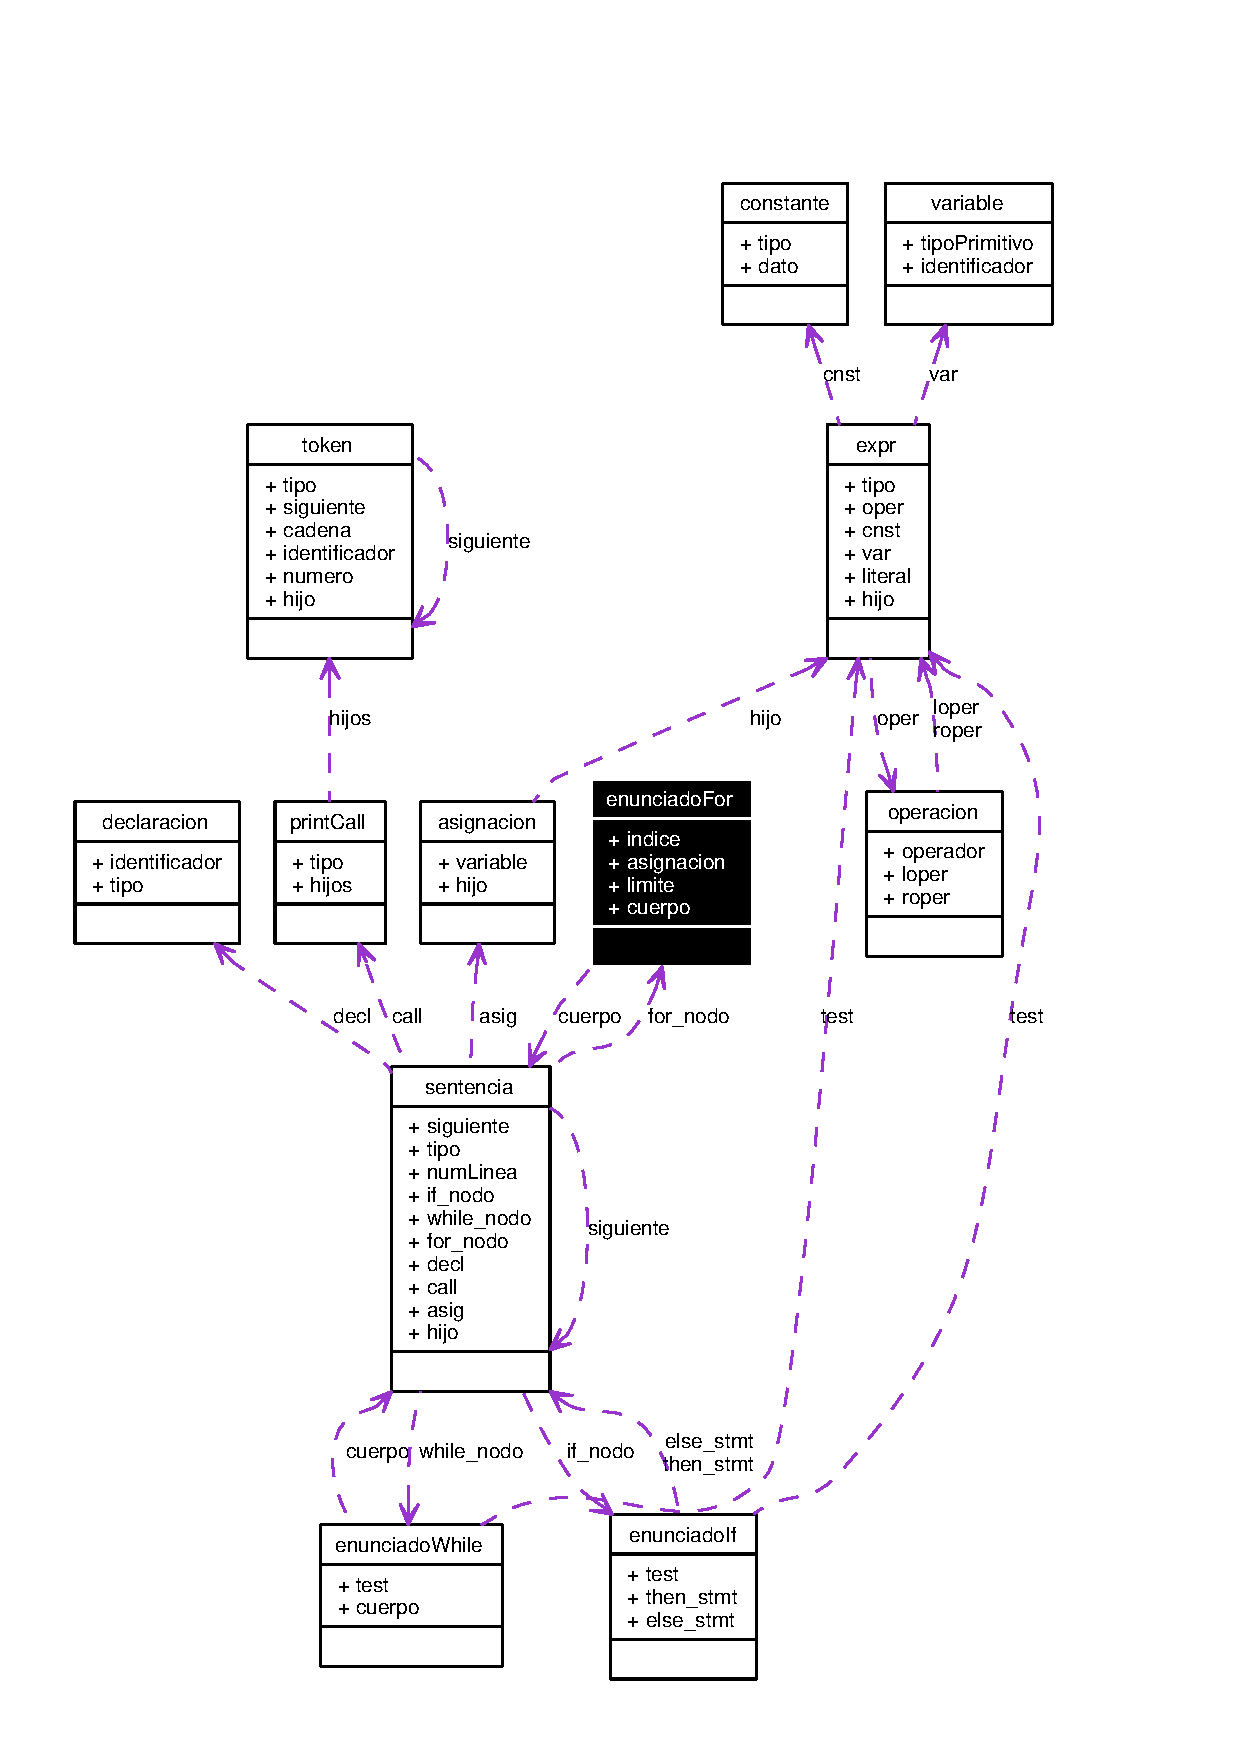
\includegraphics[width=263pt]{structenunciadoFor__coll__graph}
\end{center}
\end{figure}
\subsection*{Atributos p\'{u}blicos}
\begin{CompactItemize}
\item 
char $\ast$ {\bf indice}
\begin{CompactList}\small\item\em Identificador indice que apunta a variable entera. \item\end{CompactList}\item 
int {\bf asignacion}
\begin{CompactList}\small\item\em Entero a asignar a variable. \item\end{CompactList}\item 
int {\bf limite}
\begin{CompactList}\small\item\em Entero limite del ciclo. \item\end{CompactList}\item 
{\bf sentencia} $\ast$ {\bf cuerpo}
\begin{CompactList}\small\item\em Cuerpo de sentencias a evaluar. \item\end{CompactList}\end{CompactItemize}


\subsection{Descripci\'{o}n detallada}
Clase de almacenamiento de enunciados for en el AST. 



Definici\'{o}n en la l\'{\i}nea 197 del archivo ast.h.

\subsection{Documentaci\'{o}n de los datos miembro}
\index{enunciadoFor@{enunciado\-For}!asignacion@{asignacion}}
\index{asignacion@{asignacion}!enunciadoFor@{enunciado\-For}}
\subsubsection{\setlength{\rightskip}{0pt plus 5cm}int {\bf enunciado\-For::asignacion}}\label{structenunciadoFor_o1}


Entero a asignar a variable. 



Definici\'{o}n en la l\'{\i}nea 199 del archivo ast.h.

Referenciado por evaluar\-For(), y insertar\-Ciclo\-For().\index{enunciadoFor@{enunciado\-For}!cuerpo@{cuerpo}}
\index{cuerpo@{cuerpo}!enunciadoFor@{enunciado\-For}}
\subsubsection{\setlength{\rightskip}{0pt plus 5cm}{\bf sentencia}$\ast$ {\bf enunciado\-For::cuerpo}}\label{structenunciadoFor_o3}


Cuerpo de sentencias a evaluar. 



Definici\'{o}n en la l\'{\i}nea 201 del archivo ast.h.

Referenciado por borrar\-For(), evaluar\-For(), y insertar\-Ciclo\-For().\index{enunciadoFor@{enunciado\-For}!indice@{indice}}
\index{indice@{indice}!enunciadoFor@{enunciado\-For}}
\subsubsection{\setlength{\rightskip}{0pt plus 5cm}char$\ast$ {\bf enunciado\-For::indice}}\label{structenunciadoFor_o0}


Identificador indice que apunta a variable entera. 



Definici\'{o}n en la l\'{\i}nea 198 del archivo ast.h.

Referenciado por borrar\-For(), evaluar\-For(), y insertar\-Ciclo\-For().\index{enunciadoFor@{enunciado\-For}!limite@{limite}}
\index{limite@{limite}!enunciadoFor@{enunciado\-For}}
\subsubsection{\setlength{\rightskip}{0pt plus 5cm}int {\bf enunciado\-For::limite}}\label{structenunciadoFor_o2}


Entero limite del ciclo. 



Definici\'{o}n en la l\'{\i}nea 200 del archivo ast.h.

Referenciado por evaluar\-For(), y insertar\-Ciclo\-For().

La documentaci\'{o}n para esta estructura fu\'{e} generada a partir del siguiente archivo:\begin{CompactItemize}
\item 
/media/docs/progra/c++/compiladores1/proy2/godzilla/src/{\bf ast.h}\end{CompactItemize}

\section{Referencia de la Estructura enunciado\-If}
\label{structenunciadoIf}\index{enunciadoIf@{enunciadoIf}}
Clase de almacenamiento de enunciados If en el AST.  


{\tt \#include $<$ast.h$>$}

Diagrama de colaboraci\'{o}n para enunciado\-If:\begin{figure}[H]
\begin{center}
\leavevmode
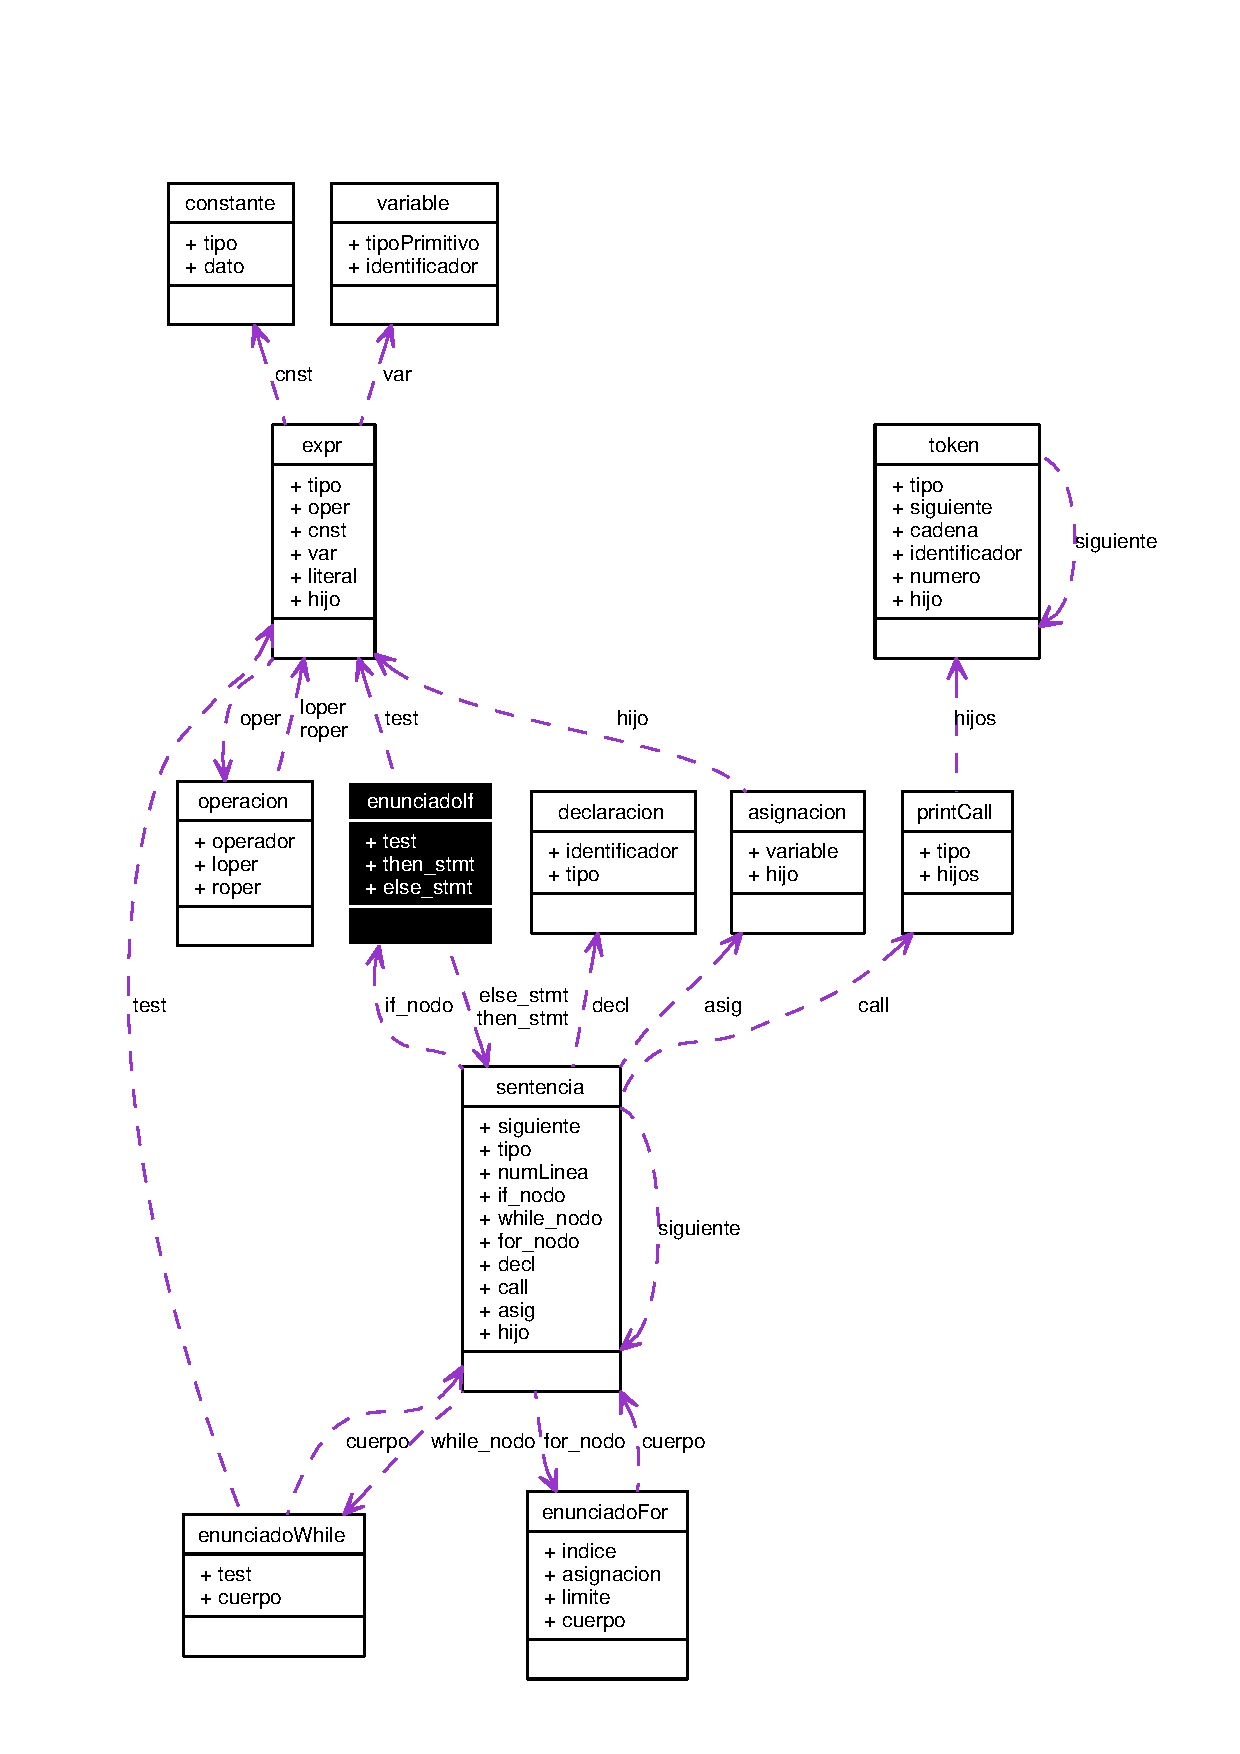
\includegraphics[width=278pt]{structenunciadoIf__coll__graph}
\end{center}
\end{figure}
\subsection*{Atributos p\'{u}blicos}
\begin{CompactItemize}
\item 
{\bf expr} $\ast$ {\bf test}
\begin{CompactList}\small\item\em Expresion booleana a evaluar (if(expr)). \item\end{CompactList}\item 
{\bf sentencia} $\ast$ {\bf then\_\-stmt}
\begin{CompactList}\small\item\em Sentencia o sentencias a evaluar en then. \item\end{CompactList}\item 
{\bf sentencia} $\ast$ {\bf else\_\-stmt}
\begin{CompactList}\small\item\em Sentencia o sentencias a evaluar en else. \item\end{CompactList}\end{CompactItemize}


\subsection{Descripci\'{o}n detallada}
Clase de almacenamiento de enunciados If en el AST. 



Definici\'{o}n en la l\'{\i}nea 186 del archivo ast.h.

\subsection{Documentaci\'{o}n de los datos miembro}
\index{enunciadoIf@{enunciado\-If}!else_stmt@{else\_\-stmt}}
\index{else_stmt@{else\_\-stmt}!enunciadoIf@{enunciado\-If}}
\subsubsection{\setlength{\rightskip}{0pt plus 5cm}{\bf sentencia}$\ast$ {\bf enunciado\-If::else\_\-stmt}}\label{structenunciadoIf_o2}


Sentencia o sentencias a evaluar en else. 



Definici\'{o}n en la l\'{\i}nea 189 del archivo ast.h.

Referenciado por borrar\-If(), evaluar\-If(), y insertar\-Enunciado\-If().\index{enunciadoIf@{enunciado\-If}!test@{test}}
\index{test@{test}!enunciadoIf@{enunciado\-If}}
\subsubsection{\setlength{\rightskip}{0pt plus 5cm}{\bf expr}$\ast$ {\bf enunciado\-If::test}}\label{structenunciadoIf_o0}


Expresion booleana a evaluar (if(expr)). 



Definici\'{o}n en la l\'{\i}nea 187 del archivo ast.h.

Referenciado por borrar\-If(), evaluar\-If(), y insertar\-Enunciado\-If().\index{enunciadoIf@{enunciado\-If}!then_stmt@{then\_\-stmt}}
\index{then_stmt@{then\_\-stmt}!enunciadoIf@{enunciado\-If}}
\subsubsection{\setlength{\rightskip}{0pt plus 5cm}{\bf sentencia}$\ast$ {\bf enunciado\-If::then\_\-stmt}}\label{structenunciadoIf_o1}


Sentencia o sentencias a evaluar en then. 



Definici\'{o}n en la l\'{\i}nea 188 del archivo ast.h.

Referenciado por borrar\-If(), evaluar\-If(), y insertar\-Enunciado\-If().

La documentaci\'{o}n para esta estructura fu\'{e} generada a partir del siguiente archivo:\begin{CompactItemize}
\item 
/media/docs/progra/c++/compiladores1/proy2/godzilla/src/{\bf ast.h}\end{CompactItemize}

\section{Referencia de la Estructura enunciado\-While}
\label{structenunciadoWhile}\index{enunciadoWhile@{enunciadoWhile}}
Clase de almacenamiento de enunciados while en el AST.  


{\tt \#include $<$ast.h$>$}

Diagrama de colaboraci\'{o}n para enunciado\-While:\begin{figure}[H]
\begin{center}
\leavevmode
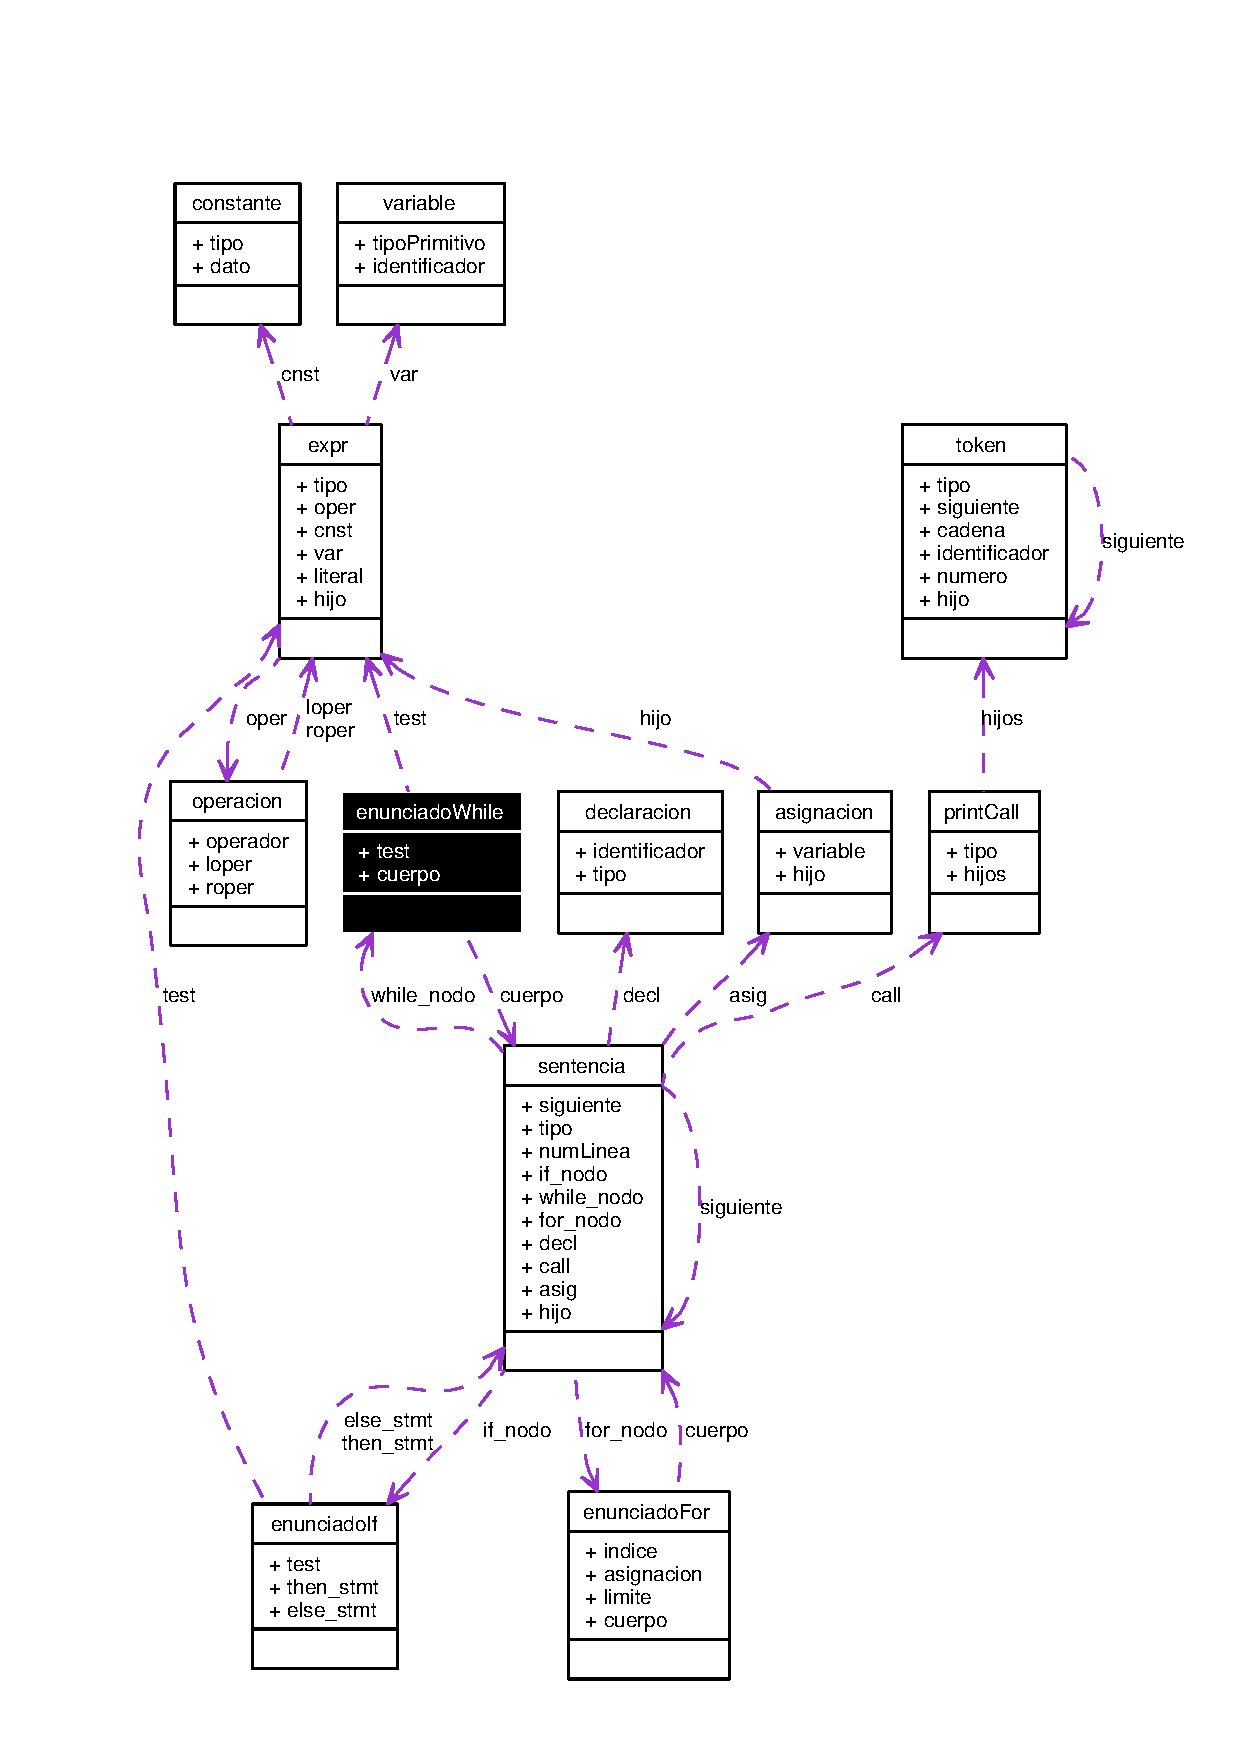
\includegraphics[width=285pt]{structenunciadoWhile__coll__graph}
\end{center}
\end{figure}
\subsection*{Atributos p\'{u}blicos}
\begin{CompactItemize}
\item 
{\bf expr} $\ast$ {\bf test}
\begin{CompactList}\small\item\em Expresion booleana a evaluar (if(expr)). \item\end{CompactList}\item 
{\bf sentencia} $\ast$ {\bf cuerpo}
\begin{CompactList}\small\item\em Cuerpo de sentencias a evaluar. \item\end{CompactList}\end{CompactItemize}


\subsection{Descripci\'{o}n detallada}
Clase de almacenamiento de enunciados while en el AST. 



Definici\'{o}n en la l\'{\i}nea 192 del archivo ast.h.

\subsection{Documentaci\'{o}n de los datos miembro}
\index{enunciadoWhile@{enunciado\-While}!cuerpo@{cuerpo}}
\index{cuerpo@{cuerpo}!enunciadoWhile@{enunciado\-While}}
\subsubsection{\setlength{\rightskip}{0pt plus 5cm}{\bf sentencia}$\ast$ {\bf enunciado\-While::cuerpo}}\label{structenunciadoWhile_o1}


Cuerpo de sentencias a evaluar. 



Definici\'{o}n en la l\'{\i}nea 194 del archivo ast.h.

Referenciado por borrar\-While(), evaluar\-While(), y insertar\-Ciclo\-While().\index{enunciadoWhile@{enunciado\-While}!test@{test}}
\index{test@{test}!enunciadoWhile@{enunciado\-While}}
\subsubsection{\setlength{\rightskip}{0pt plus 5cm}{\bf expr}$\ast$ {\bf enunciado\-While::test}}\label{structenunciadoWhile_o0}


Expresion booleana a evaluar (if(expr)). 



Definici\'{o}n en la l\'{\i}nea 193 del archivo ast.h.

Referenciado por borrar\-While(), evaluar\-While(), y insertar\-Ciclo\-While().

La documentaci\'{o}n para esta estructura fu\'{e} generada a partir del siguiente archivo:\begin{CompactItemize}
\item 
/media/docs/progra/c++/compiladores1/proy2/godzilla/src/{\bf ast.h}\end{CompactItemize}

\section{Referencia de la Estructura expr}
\label{structexpr}\index{expr@{expr}}
Clase de almacenamiento de raiz de un arbol de expresiones en el AST.  


{\tt \#include $<$ast.h$>$}

Diagrama de colaboraci\'{o}n para expr:\begin{figure}[H]
\begin{center}
\leavevmode
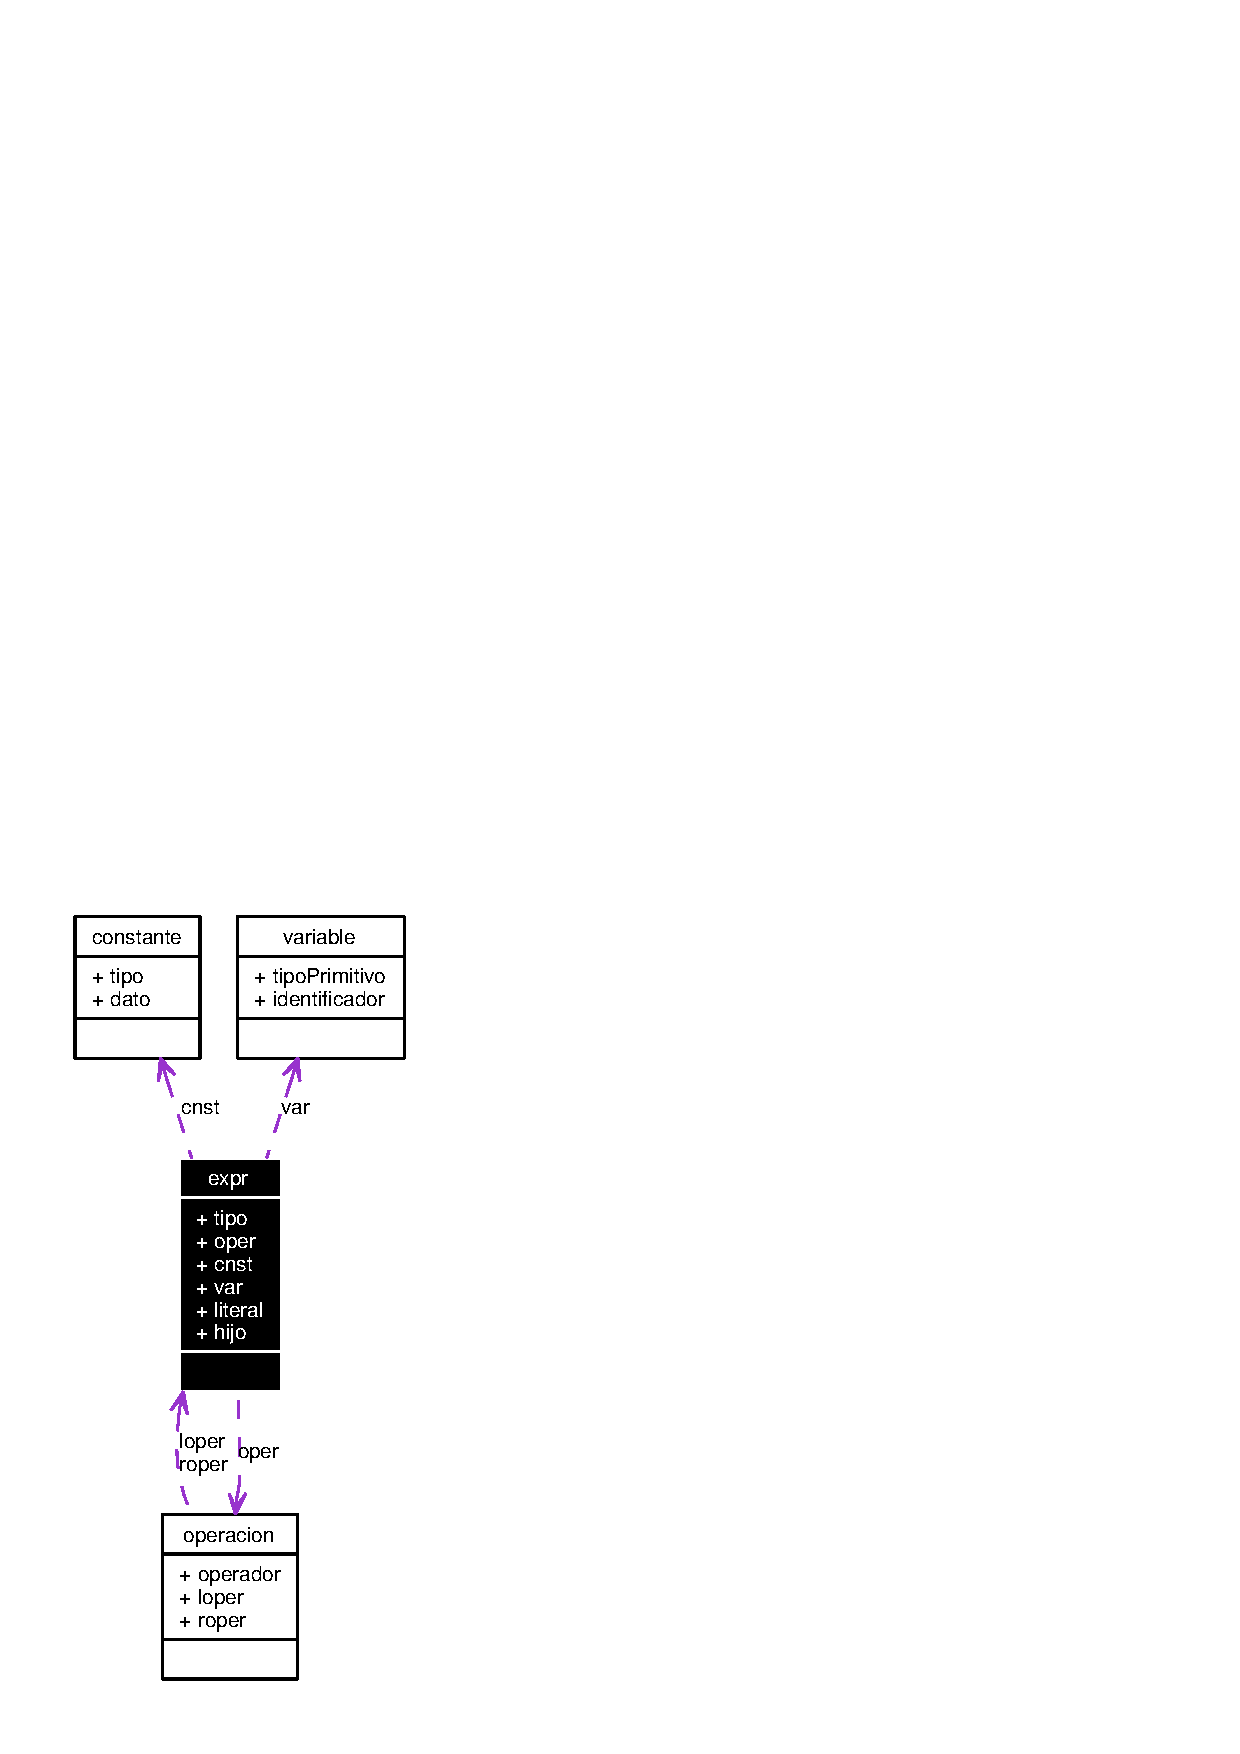
\includegraphics[width=97pt]{structexpr__coll__graph}
\end{center}
\end{figure}
\subsection*{Atributos p\'{u}blicos}
\begin{CompactItemize}
\item 
int {\bf tipo}
\begin{CompactList}\small\item\em Tipo de expresion. \item\end{CompactList}\item 
\begin{tabbing}
xx\=xx\=xx\=xx\=xx\=xx\=xx\=xx\=xx\=\kill
union \{\\
\>{\bf operacion} $\ast$ {\bf oper}\\
\>{\bf constante} $\ast$ {\bf cnst}\\
\>{\bf variable} $\ast$ {\bf var}\\
\>char $\ast$ {\bf literal}\\
\} {\bf hijo}\\

\end{tabbing}\begin{CompactList}\small\item\em Puntero a dato correspondiente. \item\end{CompactList}\end{CompactItemize}


\subsection{Descripci\'{o}n detallada}
Clase de almacenamiento de raiz de un arbol de expresiones en el AST. 



Definici\'{o}n en la l\'{\i}nea 205 del archivo ast.h.

\subsection{Documentaci\'{o}n de los datos miembro}
\index{expr@{expr}!cnst@{cnst}}
\index{cnst@{cnst}!expr@{expr}}
\subsubsection{\setlength{\rightskip}{0pt plus 5cm}{\bf constante}$\ast$ {\bf expr::cnst}}\label{structexpr_o2}




Definici\'{o}n en la l\'{\i}nea 209 del archivo ast.h.\index{expr@{expr}!hijo@{hijo}}
\index{hijo@{hijo}!expr@{expr}}
\subsubsection{\setlength{\rightskip}{0pt plus 5cm}union \{ ... \}  {\bf expr::hijo}}\label{structexpr_o5}


Puntero a dato correspondiente. 



Referenciado por borrar\-Expresion(), evaluar\-Expresion(), insertar\-Cadena(), y insertar\-Expresion().\index{expr@{expr}!literal@{literal}}
\index{literal@{literal}!expr@{expr}}
\subsubsection{\setlength{\rightskip}{0pt plus 5cm}char$\ast$ {\bf expr::literal}}\label{structexpr_o4}




Definici\'{o}n en la l\'{\i}nea 211 del archivo ast.h.\index{expr@{expr}!oper@{oper}}
\index{oper@{oper}!expr@{expr}}
\subsubsection{\setlength{\rightskip}{0pt plus 5cm}{\bf operacion}$\ast$ {\bf expr::oper}}\label{structexpr_o1}




Definici\'{o}n en la l\'{\i}nea 208 del archivo ast.h.\index{expr@{expr}!tipo@{tipo}}
\index{tipo@{tipo}!expr@{expr}}
\subsubsection{\setlength{\rightskip}{0pt plus 5cm}int {\bf expr::tipo}}\label{structexpr_o0}


Tipo de expresion. 



Definici\'{o}n en la l\'{\i}nea 206 del archivo ast.h.

Referenciado por borrar\-Expresion(), evaluar\-Expresion(), insertar\-Cadena(), y insertar\-Expresion().\index{expr@{expr}!var@{var}}
\index{var@{var}!expr@{expr}}
\subsubsection{\setlength{\rightskip}{0pt plus 5cm}{\bf variable}$\ast$ {\bf expr::var}}\label{structexpr_o3}




Definici\'{o}n en la l\'{\i}nea 210 del archivo ast.h.

La documentaci\'{o}n para esta estructura fu\'{e} generada a partir del siguiente archivo:\begin{CompactItemize}
\item 
/media/docs/progra/c++/compiladores1/proy2/godzilla/src/{\bf ast.h}\end{CompactItemize}

\section{Referencia de la Clase God\-Zilla}
\label{classGodZilla}\index{GodZilla@{GodZilla}}
{\tt \#include $<$godzilla.h$>$}

Diagrama de colaboraci\'{o}n para God\-Zilla:\begin{figure}[H]
\begin{center}
\leavevmode
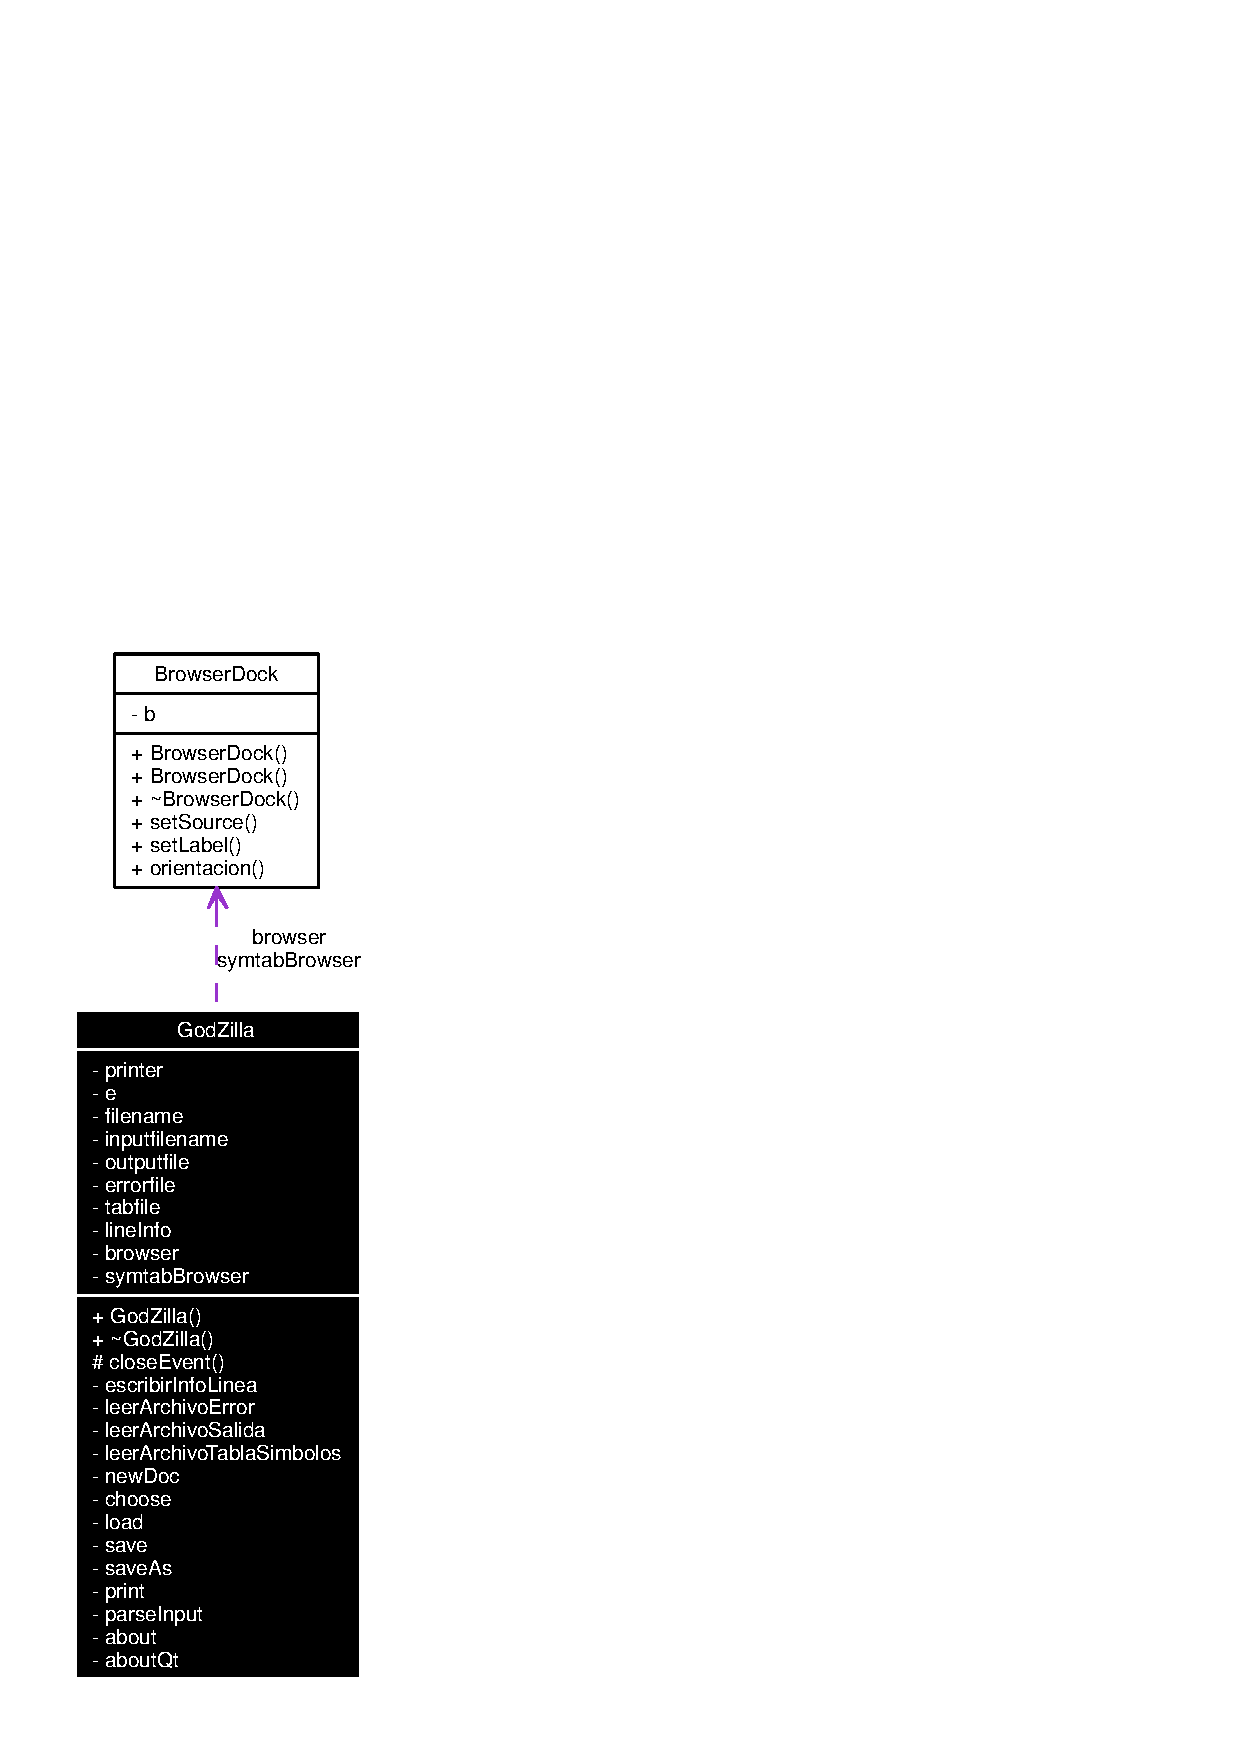
\includegraphics[width=87pt]{classGodZilla__coll__graph}
\end{center}
\end{figure}
\subsection*{M\'{e}todos p\'{u}blicos}
\begin{CompactItemize}
\item 
{\bf God\-Zilla} ()
\item 
{\bf $\sim$God\-Zilla} ()
\end{CompactItemize}
\subsection*{M\'{e}todos protegidos}
\begin{CompactItemize}
\item 
void {\bf close\-Event} (QClose\-Event $\ast$)
\end{CompactItemize}
\subsection*{Slots privados}
\begin{CompactItemize}
\item 
void {\bf escribir\-Info\-Linea} (int row, int col)
\begin{CompactList}\small\item\em slot para escribir linea de archivo al widget line\-Info contenido en la barra de estados \item\end{CompactList}\item 
void {\bf leer\-Archivo\-Error} ()
\begin{CompactList}\small\item\em Abre en el browser el archivo de error. \item\end{CompactList}\item 
void {\bf leer\-Archivo\-Salida} ()
\begin{CompactList}\small\item\em Abre en el browser el archivo de salida. \item\end{CompactList}\item 
void {\bf leer\-Archivo\-Tabla\-Simbolos} ()
\begin{CompactList}\small\item\em Abre en el browser el archivo de tabla de simbolos. \item\end{CompactList}\item 
void {\bf new\-Doc} ()
\item 
void {\bf choose} ()
\item 
void {\bf load} (const QString \&file\-Name)
\item 
void {\bf save} ()
\item 
void {\bf save\-As} ()
\item 
void {\bf print} ()
\begin{CompactList}\small\item\em Llama al modulo de impresion del shell. \item\end{CompactList}\item 
int {\bf parse\-Input} ()
\begin{CompactList}\small\item\em Slot para el boton de analisis del archivo de entrada. \item\end{CompactList}\item 
void {\bf about} ()
\begin{CompactList}\small\item\em Muestra dialogo. \item\end{CompactList}\item 
void {\bf about\-Qt} ()
\end{CompactItemize}
\subsection*{Atributos privados}
\begin{CompactItemize}
\item 
QPrinter $\ast$ {\bf printer}
\item 
QText\-Edit $\ast$ {\bf e}
\item 
QString {\bf filename}
\item 
QString {\bf inputfilename}
\item 
QString {\bf outputfile}
\item 
QString {\bf errorfile}
\item 
QString {\bf tabfile}
\item 
QLabel $\ast$ {\bf line\-Info}
\item 
{\bf Browser\-Dock} $\ast$ {\bf browser}
\item 
{\bf Browser\-Dock} $\ast$ {\bf symtab\-Browser}
\end{CompactItemize}


\subsection{Descripci\'{o}n detallada}




Definici\'{o}n en la l\'{\i}nea 30 del archivo godzilla.h.

\subsection{Documentaci\'{o}n del constructor y destructor}
\index{GodZilla@{God\-Zilla}!GodZilla@{GodZilla}}
\index{GodZilla@{GodZilla}!GodZilla@{God\-Zilla}}
\subsubsection{\setlength{\rightskip}{0pt plus 5cm}God\-Zilla::God\-Zilla ()}\label{classGodZilla_a0}




Definici\'{o}n en la l\'{\i}nea 33 del archivo godzilla.cpp.

Hace referencia a about(), about\-Qt(), browser, choose(), e, escribir\-Info\-Linea(), leer\-Archivo\-Error(), leer\-Archivo\-Salida(), leer\-Archivo\-Tabla\-Simbolos(), line\-Info, new\-Doc(), parse\-Input(), print(), printer, save(), save\-As(), y Browser\-Dock::set\-Label().\index{GodZilla@{God\-Zilla}!~GodZilla@{$\sim$GodZilla}}
\index{~GodZilla@{$\sim$GodZilla}!GodZilla@{God\-Zilla}}
\subsubsection{\setlength{\rightskip}{0pt plus 5cm}God\-Zilla::$\sim$God\-Zilla ()}\label{classGodZilla_a1}




Definici\'{o}n en la l\'{\i}nea 186 del archivo godzilla.cpp.

Hace referencia a printer.

\subsection{Documentaci\'{o}n de las funciones miembro}
\index{GodZilla@{God\-Zilla}!about@{about}}
\index{about@{about}!GodZilla@{God\-Zilla}}
\subsubsection{\setlength{\rightskip}{0pt plus 5cm}void God\-Zilla::about ()\hspace{0.3cm}{\tt  [private, slot]}}\label{classGodZilla_k11}


Muestra dialogo. 



Definici\'{o}n en la l\'{\i}nea 413 del archivo godzilla.cpp.

Referenciado por God\-Zilla().\index{GodZilla@{God\-Zilla}!aboutQt@{aboutQt}}
\index{aboutQt@{aboutQt}!GodZilla@{God\-Zilla}}
\subsubsection{\setlength{\rightskip}{0pt plus 5cm}void God\-Zilla::about\-Qt ()\hspace{0.3cm}{\tt  [private, slot]}}\label{classGodZilla_k12}




Definici\'{o}n en la l\'{\i}nea 422 del archivo godzilla.cpp.

Referenciado por God\-Zilla().\index{GodZilla@{God\-Zilla}!choose@{choose}}
\index{choose@{choose}!GodZilla@{God\-Zilla}}
\subsubsection{\setlength{\rightskip}{0pt plus 5cm}void God\-Zilla::choose ()\hspace{0.3cm}{\tt  [private, slot]}}\label{classGodZilla_k5}




Definici\'{o}n en la l\'{\i}nea 199 del archivo godzilla.cpp.

Hace referencia a load().

Referenciado por God\-Zilla().\index{GodZilla@{God\-Zilla}!closeEvent@{closeEvent}}
\index{closeEvent@{closeEvent}!GodZilla@{God\-Zilla}}
\subsubsection{\setlength{\rightskip}{0pt plus 5cm}void God\-Zilla::close\-Event (QClose\-Event $\ast$)\hspace{0.3cm}{\tt  [protected]}}\label{classGodZilla_b0}




Definici\'{o}n en la l\'{\i}nea 386 del archivo godzilla.cpp.

Hace referencia a e, y save().\index{GodZilla@{God\-Zilla}!escribirInfoLinea@{escribirInfoLinea}}
\index{escribirInfoLinea@{escribirInfoLinea}!GodZilla@{God\-Zilla}}
\subsubsection{\setlength{\rightskip}{0pt plus 5cm}void God\-Zilla::escribir\-Info\-Linea (int {\em row}, int {\em col})\hspace{0.3cm}{\tt  [private, slot]}}\label{classGodZilla_k0}


slot para escribir linea de archivo al widget line\-Info contenido en la barra de estados 



Definici\'{o}n en la l\'{\i}nea 320 del archivo godzilla.cpp.

Hace referencia a line\-Info.

Referenciado por God\-Zilla().\index{GodZilla@{God\-Zilla}!leerArchivoError@{leerArchivoError}}
\index{leerArchivoError@{leerArchivoError}!GodZilla@{God\-Zilla}}
\subsubsection{\setlength{\rightskip}{0pt plus 5cm}void God\-Zilla::leer\-Archivo\-Error ()\hspace{0.3cm}{\tt  [private, slot]}}\label{classGodZilla_k1}


Abre en el browser el archivo de error. 



Definici\'{o}n en la l\'{\i}nea 324 del archivo godzilla.cpp.

Hace referencia a browser, errorfile, y Browser\-Dock::set\-Source().

Referenciado por God\-Zilla().\index{GodZilla@{God\-Zilla}!leerArchivoSalida@{leerArchivoSalida}}
\index{leerArchivoSalida@{leerArchivoSalida}!GodZilla@{God\-Zilla}}
\subsubsection{\setlength{\rightskip}{0pt plus 5cm}void God\-Zilla::leer\-Archivo\-Salida ()\hspace{0.3cm}{\tt  [private, slot]}}\label{classGodZilla_k2}


Abre en el browser el archivo de salida. 



Definici\'{o}n en la l\'{\i}nea 338 del archivo godzilla.cpp.

Hace referencia a browser, outputfile, y Browser\-Dock::set\-Source().

Referenciado por God\-Zilla().\index{GodZilla@{God\-Zilla}!leerArchivoTablaSimbolos@{leerArchivoTablaSimbolos}}
\index{leerArchivoTablaSimbolos@{leerArchivoTablaSimbolos}!GodZilla@{God\-Zilla}}
\subsubsection{\setlength{\rightskip}{0pt plus 5cm}void God\-Zilla::leer\-Archivo\-Tabla\-Simbolos ()\hspace{0.3cm}{\tt  [private, slot]}}\label{classGodZilla_k3}


Abre en el browser el archivo de tabla de simbolos. 



Definici\'{o}n en la l\'{\i}nea 331 del archivo godzilla.cpp.

Hace referencia a browser, outputfile, y Browser\-Dock::set\-Source().

Referenciado por God\-Zilla().\index{GodZilla@{God\-Zilla}!load@{load}}
\index{load@{load}!GodZilla@{God\-Zilla}}
\subsubsection{\setlength{\rightskip}{0pt plus 5cm}void God\-Zilla::load (const QString \& {\em file\-Name})\hspace{0.3cm}{\tt  [private, slot]}}\label{classGodZilla_k6}




Definici\'{o}n en la l\'{\i}nea 210 del archivo godzilla.cpp.

Hace referencia a e, filename, y inputfilename.

Referenciado por choose().\index{GodZilla@{God\-Zilla}!newDoc@{newDoc}}
\index{newDoc@{newDoc}!GodZilla@{God\-Zilla}}
\subsubsection{\setlength{\rightskip}{0pt plus 5cm}void God\-Zilla::new\-Doc ()\hspace{0.3cm}{\tt  [private, slot]}}\label{classGodZilla_k4}




Definici\'{o}n en la l\'{\i}nea 192 del archivo godzilla.cpp.

Referenciado por God\-Zilla().\index{GodZilla@{God\-Zilla}!parseInput@{parseInput}}
\index{parseInput@{parseInput}!GodZilla@{God\-Zilla}}
\subsubsection{\setlength{\rightskip}{0pt plus 5cm}int God\-Zilla::parse\-Input ()\hspace{0.3cm}{\tt  [private, slot]}}\label{classGodZilla_k10}


Slot para el boton de analisis del archivo de entrada. 



Definici\'{o}n en la l\'{\i}nea 273 del archivo godzilla.cpp.

Hace referencia a browser, errorfile, generar\-Salida\-Error(), inputfilename, inputparse(), outputfile, Browser\-Dock::set\-Source(), y tabfile.

Referenciado por God\-Zilla().\index{GodZilla@{God\-Zilla}!print@{print}}
\index{print@{print}!GodZilla@{God\-Zilla}}
\subsubsection{\setlength{\rightskip}{0pt plus 5cm}void God\-Zilla::print ()\hspace{0.3cm}{\tt  [private, slot]}}\label{classGodZilla_k9}


Llama al modulo de impresion del shell. 



Definici\'{o}n en la l\'{\i}nea 347 del archivo godzilla.cpp.

Hace referencia a e, y printer.

Referenciado por God\-Zilla().\index{GodZilla@{God\-Zilla}!save@{save}}
\index{save@{save}!GodZilla@{God\-Zilla}}
\subsubsection{\setlength{\rightskip}{0pt plus 5cm}void God\-Zilla::save ()\hspace{0.3cm}{\tt  [private, slot]}}\label{classGodZilla_k7}




Definici\'{o}n en la l\'{\i}nea 228 del archivo godzilla.cpp.

Hace referencia a e, filename, inputfilename, y save\-As().

Referenciado por close\-Event(), God\-Zilla(), y save\-As().\index{GodZilla@{God\-Zilla}!saveAs@{saveAs}}
\index{saveAs@{saveAs}!GodZilla@{God\-Zilla}}
\subsubsection{\setlength{\rightskip}{0pt plus 5cm}void God\-Zilla::save\-As ()\hspace{0.3cm}{\tt  [private, slot]}}\label{classGodZilla_k8}




Definici\'{o}n en la l\'{\i}nea 255 del archivo godzilla.cpp.

Hace referencia a filename, inputfilename, y save().

Referenciado por God\-Zilla(), y save().

\subsection{Documentaci\'{o}n de los datos miembro}
\index{GodZilla@{God\-Zilla}!browser@{browser}}
\index{browser@{browser}!GodZilla@{God\-Zilla}}
\subsubsection{\setlength{\rightskip}{0pt plus 5cm}{\bf Browser\-Dock}$\ast$ {\bf God\-Zilla::browser}\hspace{0.3cm}{\tt  [private]}}\label{classGodZilla_r8}




Definici\'{o}n en la l\'{\i}nea 68 del archivo godzilla.h.

Referenciado por God\-Zilla(), leer\-Archivo\-Error(), leer\-Archivo\-Salida(), leer\-Archivo\-Tabla\-Simbolos(), y parse\-Input().\index{GodZilla@{God\-Zilla}!e@{e}}
\index{e@{e}!GodZilla@{God\-Zilla}}
\subsubsection{\setlength{\rightskip}{0pt plus 5cm}QText\-Edit$\ast$ {\bf God\-Zilla::e}\hspace{0.3cm}{\tt  [private]}}\label{classGodZilla_r1}




Definici\'{o}n en la l\'{\i}nea 61 del archivo godzilla.h.

Referenciado por close\-Event(), God\-Zilla(), load(), print(), y save().\index{GodZilla@{God\-Zilla}!errorfile@{errorfile}}
\index{errorfile@{errorfile}!GodZilla@{God\-Zilla}}
\subsubsection{\setlength{\rightskip}{0pt plus 5cm}QString {\bf God\-Zilla::errorfile}\hspace{0.3cm}{\tt  [private]}}\label{classGodZilla_r5}




Definici\'{o}n en la l\'{\i}nea 65 del archivo godzilla.h.

Referenciado por leer\-Archivo\-Error(), y parse\-Input().\index{GodZilla@{God\-Zilla}!filename@{filename}}
\index{filename@{filename}!GodZilla@{God\-Zilla}}
\subsubsection{\setlength{\rightskip}{0pt plus 5cm}QString {\bf God\-Zilla::filename}\hspace{0.3cm}{\tt  [private]}}\label{classGodZilla_r2}




Definici\'{o}n en la l\'{\i}nea 62 del archivo godzilla.h.

Referenciado por load(), save(), y save\-As().\index{GodZilla@{God\-Zilla}!inputfilename@{inputfilename}}
\index{inputfilename@{inputfilename}!GodZilla@{God\-Zilla}}
\subsubsection{\setlength{\rightskip}{0pt plus 5cm}QString {\bf God\-Zilla::inputfilename}\hspace{0.3cm}{\tt  [private]}}\label{classGodZilla_r3}




Definici\'{o}n en la l\'{\i}nea 63 del archivo godzilla.h.

Referenciado por load(), parse\-Input(), save(), y save\-As().\index{GodZilla@{God\-Zilla}!lineInfo@{lineInfo}}
\index{lineInfo@{lineInfo}!GodZilla@{God\-Zilla}}
\subsubsection{\setlength{\rightskip}{0pt plus 5cm}QLabel$\ast$ {\bf God\-Zilla::line\-Info}\hspace{0.3cm}{\tt  [private]}}\label{classGodZilla_r7}




Definici\'{o}n en la l\'{\i}nea 67 del archivo godzilla.h.

Referenciado por escribir\-Info\-Linea(), y God\-Zilla().\index{GodZilla@{God\-Zilla}!outputfile@{outputfile}}
\index{outputfile@{outputfile}!GodZilla@{God\-Zilla}}
\subsubsection{\setlength{\rightskip}{0pt plus 5cm}QString {\bf God\-Zilla::outputfile}\hspace{0.3cm}{\tt  [private]}}\label{classGodZilla_r4}




Definici\'{o}n en la l\'{\i}nea 64 del archivo godzilla.h.

Referenciado por leer\-Archivo\-Salida(), leer\-Archivo\-Tabla\-Simbolos(), y parse\-Input().\index{GodZilla@{God\-Zilla}!printer@{printer}}
\index{printer@{printer}!GodZilla@{God\-Zilla}}
\subsubsection{\setlength{\rightskip}{0pt plus 5cm}QPrinter$\ast$ {\bf God\-Zilla::printer}\hspace{0.3cm}{\tt  [private]}}\label{classGodZilla_r0}




Definici\'{o}n en la l\'{\i}nea 60 del archivo godzilla.h.

Referenciado por God\-Zilla(), print(), y $\sim$God\-Zilla().\index{GodZilla@{God\-Zilla}!symtabBrowser@{symtabBrowser}}
\index{symtabBrowser@{symtabBrowser}!GodZilla@{God\-Zilla}}
\subsubsection{\setlength{\rightskip}{0pt plus 5cm}{\bf Browser\-Dock}$\ast$ {\bf God\-Zilla::symtab\-Browser}\hspace{0.3cm}{\tt  [private]}}\label{classGodZilla_r9}




Definici\'{o}n en la l\'{\i}nea 69 del archivo godzilla.h.\index{GodZilla@{God\-Zilla}!tabfile@{tabfile}}
\index{tabfile@{tabfile}!GodZilla@{God\-Zilla}}
\subsubsection{\setlength{\rightskip}{0pt plus 5cm}QString {\bf God\-Zilla::tabfile}\hspace{0.3cm}{\tt  [private]}}\label{classGodZilla_r6}




Definici\'{o}n en la l\'{\i}nea 66 del archivo godzilla.h.

Referenciado por parse\-Input().

La documentaci\'{o}n para esta clase fu\'{e} generada a partir de los siguientes archivos:\begin{CompactItemize}
\item 
/media/docs/progra/c++/compiladores1/proy2/godzilla/src/{\bf godzilla.h}\item 
/media/docs/progra/c++/compiladores1/proy2/godzilla/src/{\bf godzilla.cpp}\end{CompactItemize}

\section{Referencia de la Estructura nodo\-Cola\-Err}
\label{structnodoColaErr}\index{nodoColaErr@{nodoColaErr}}
Nodo de la cola de errores.  


{\tt \#include $<$colaerr.h$>$}

Diagrama de colaboraci\'{o}n para nodo\-Cola\-Err:\begin{figure}[H]
\begin{center}
\leavevmode
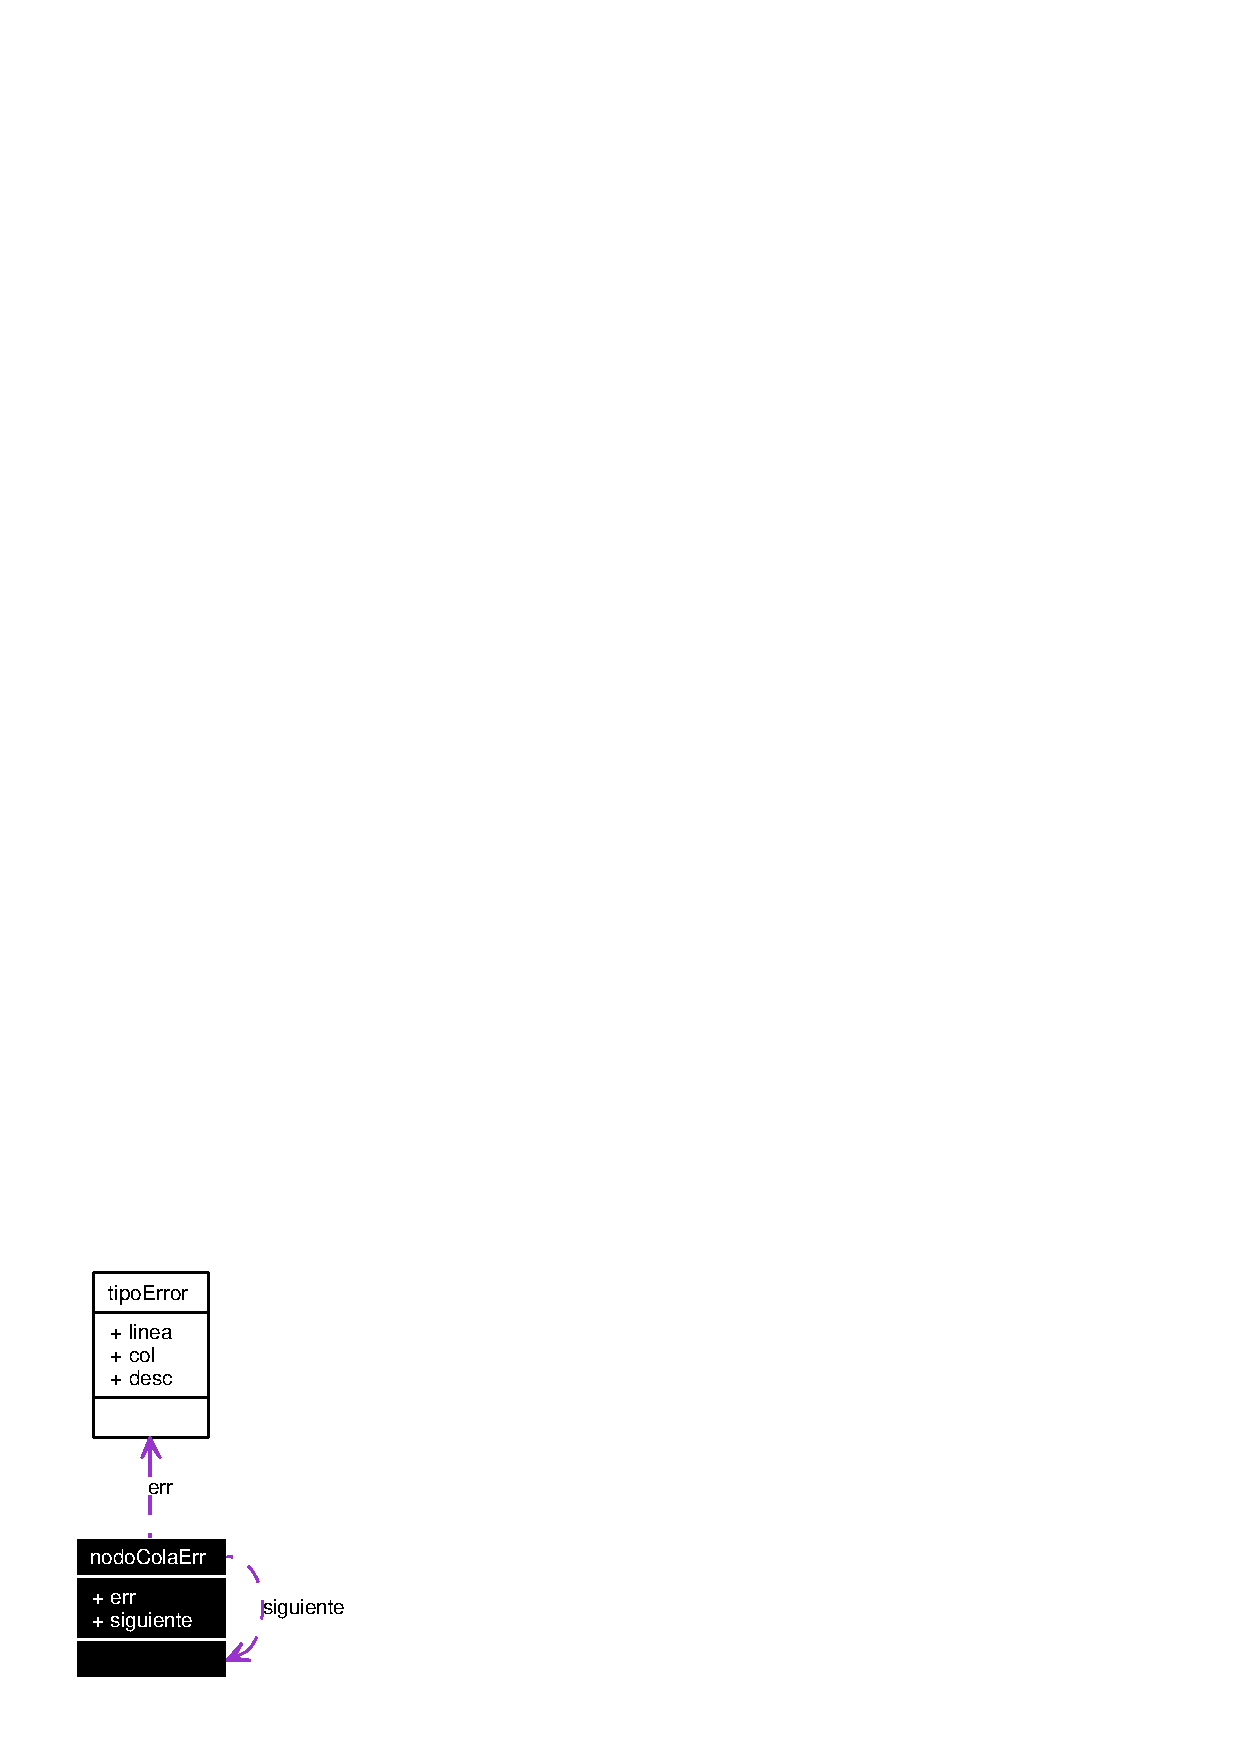
\includegraphics[width=83pt]{structnodoColaErr__coll__graph}
\end{center}
\end{figure}
\subsection*{Atributos p\'{u}blicos}
\begin{CompactItemize}
\item 
{\bf tipo\-Error} $\ast$ {\bf err}
\item 
{\bf nodo\-Cola\-Err} $\ast$ {\bf siguiente}
\end{CompactItemize}


\subsection{Descripci\'{o}n detallada}
Nodo de la cola de errores. 



Definici\'{o}n en la l\'{\i}nea 34 del archivo colaerr.h.

\subsection{Documentaci\'{o}n de los datos miembro}
\index{nodoColaErr@{nodo\-Cola\-Err}!err@{err}}
\index{err@{err}!nodoColaErr@{nodo\-Cola\-Err}}
\subsubsection{\setlength{\rightskip}{0pt plus 5cm}{\bf tipo\-Error}$\ast$ {\bf nodo\-Cola\-Err::err}}\label{structnodoColaErr_o0}




Definici\'{o}n en la l\'{\i}nea 35 del archivo colaerr.h.

Referenciado por encolar\-Error(), y sacar\-Error().\index{nodoColaErr@{nodo\-Cola\-Err}!siguiente@{siguiente}}
\index{siguiente@{siguiente}!nodoColaErr@{nodo\-Cola\-Err}}
\subsubsection{\setlength{\rightskip}{0pt plus 5cm}{\bf nodo\-Cola\-Err}$\ast$ {\bf nodo\-Cola\-Err::siguiente}}\label{structnodoColaErr_o1}




Definici\'{o}n en la l\'{\i}nea 36 del archivo colaerr.h.

Referenciado por encolar\-Error(), y sacar\-Error().

La documentaci\'{o}n para esta estructura fu\'{e} generada a partir del siguiente archivo:\begin{CompactItemize}
\item 
/media/docs/progra/c++/compiladores1/proy2/godzilla/src/{\bf colaerr.h}\end{CompactItemize}

\section{Referencia de la Estructura nodo\-Hijo}
\label{structnodoHijo}\index{nodoHijo@{nodoHijo}}
Nodo a usar para pasar entre producciones de la sintaxis, y paso de expresiones al recorrer un arbol de expresiones.  


{\tt \#include $<$ast.h$>$}

\subsection*{Atributos p\'{u}blicos}
\begin{CompactItemize}
\item 
int {\bf tipo}
\begin{CompactList}\small\item\em Tipo de nodo. \item\end{CompactList}\item 
void $\ast$ {\bf dato}
\begin{CompactList}\small\item\em Dato del nodo. \item\end{CompactList}\end{CompactItemize}


\subsection{Descripci\'{o}n detallada}
Nodo a usar para pasar entre producciones de la sintaxis, y paso de expresiones al recorrer un arbol de expresiones. 



Definici\'{o}n en la l\'{\i}nea 259 del archivo ast.h.

\subsection{Documentaci\'{o}n de los datos miembro}
\index{nodoHijo@{nodo\-Hijo}!dato@{dato}}
\index{dato@{dato}!nodoHijo@{nodo\-Hijo}}
\subsubsection{\setlength{\rightskip}{0pt plus 5cm}void$\ast$ {\bf nodo\-Hijo::dato}}\label{structnodoHijo_o1}


Dato del nodo. 



Definici\'{o}n en la l\'{\i}nea 261 del archivo ast.h.

Referenciado por concatenar\-Sentencia(), concatenar\-Tokens(), crear\-Raiz(), evaluar\-And(), evaluar\-Asignacion(), evaluar\-Div(), evaluar\-EQ(), evaluar\-Expresion(), evaluar\-GET(), evaluar\-GT(), evaluar\-If(), evaluar\-LET(), evaluar\-LT(), evaluar\-Mult(), evaluar\-NEQ(), evaluar\-Or(), evaluar\-Resta(), evaluar\-Suma(), evaluar\-While(), insertar\-Asignacion(), insertar\-Ciclo\-For(), insertar\-Ciclo\-While(), insertar\-Enunciado\-If(), insertar\-Expresion(), insertar\-Llamada(), insertar\-Operacion(), insertar\-Sentencia(), y ref\-Nodo\-Hijo().\index{nodoHijo@{nodo\-Hijo}!tipo@{tipo}}
\index{tipo@{tipo}!nodoHijo@{nodo\-Hijo}}
\subsubsection{\setlength{\rightskip}{0pt plus 5cm}int {\bf nodo\-Hijo::tipo}}\label{structnodoHijo_o0}


Tipo de nodo. 



Definici\'{o}n en la l\'{\i}nea 260 del archivo ast.h.

Referenciado por evaluar\-And(), evaluar\-Asignacion(), evaluar\-Div(), evaluar\-EQ(), evaluar\-Expresion(), evaluar\-GET(), evaluar\-GT(), evaluar\-If(), evaluar\-LET(), evaluar\-LT(), evaluar\-Mult(), evaluar\-NEQ(), evaluar\-Or(), evaluar\-Resta(), evaluar\-Suma(), evaluar\-While(), insertar\-Expresion(), y ref\-Nodo\-Hijo().

La documentaci\'{o}n para esta estructura fu\'{e} generada a partir del siguiente archivo:\begin{CompactItemize}
\item 
/media/docs/progra/c++/compiladores1/proy2/godzilla/src/{\bf ast.h}\end{CompactItemize}

\section{Referencia de la Estructura operacion}
\label{structoperacion}\index{operacion@{operacion}}
Clase de almacenamiento de operaciones en el AST.  


{\tt \#include $<$ast.h$>$}

Diagrama de colaboraci\'{o}n para operacion:\begin{figure}[H]
\begin{center}
\leavevmode
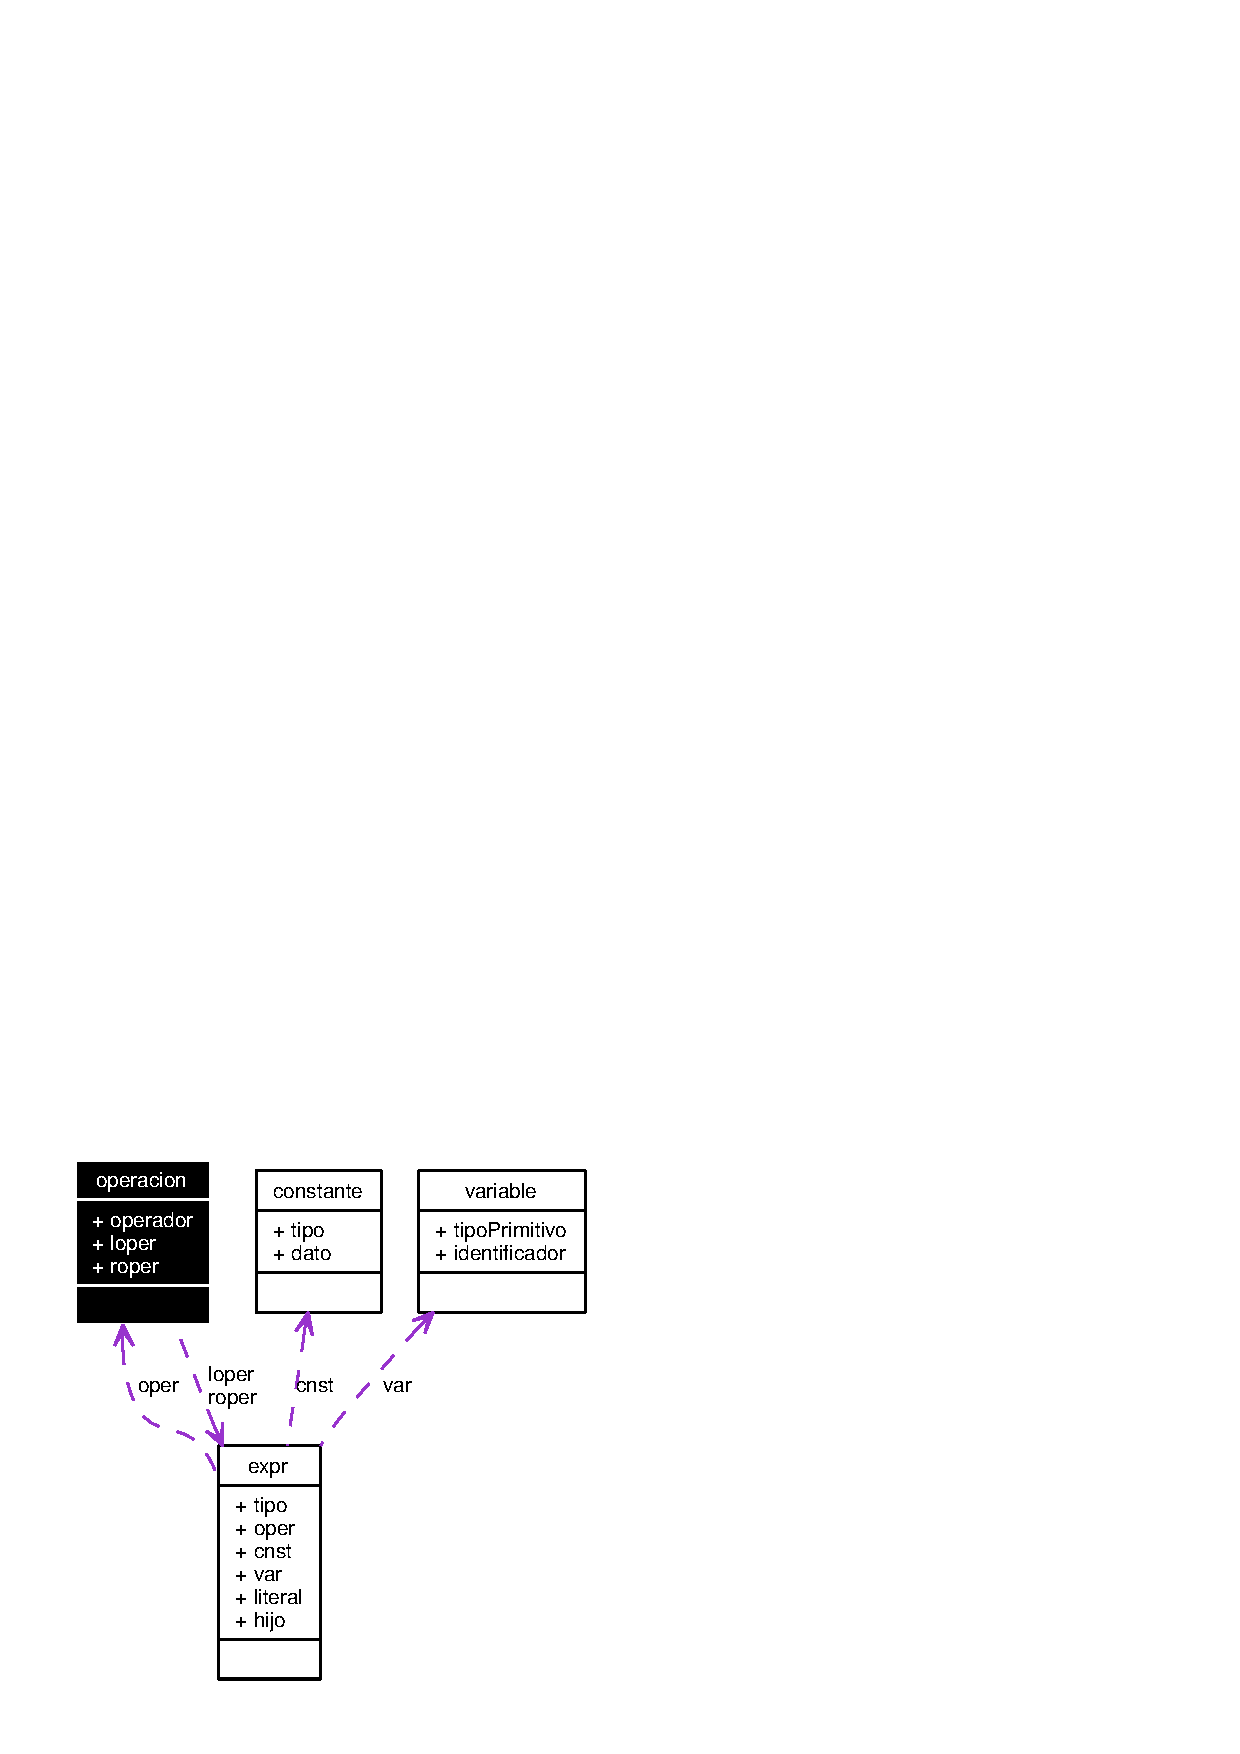
\includegraphics[width=141pt]{structoperacion__coll__graph}
\end{center}
\end{figure}
\subsection*{Atributos p\'{u}blicos}
\begin{CompactItemize}
\item 
int {\bf operador}
\begin{CompactList}\small\item\em Operador. \item\end{CompactList}\item 
{\bf expr} $\ast$ {\bf loper}
\begin{CompactList}\small\item\em Expresion a la izquierda del operador. \item\end{CompactList}\item 
{\bf expr} $\ast$ {\bf roper}
\begin{CompactList}\small\item\em Expresion a la derecha del operador. \item\end{CompactList}\end{CompactItemize}


\subsection{Descripci\'{o}n detallada}
Clase de almacenamiento de operaciones en el AST. 



Definici\'{o}n en la l\'{\i}nea 180 del archivo ast.h.

\subsection{Documentaci\'{o}n de los datos miembro}
\index{operacion@{operacion}!loper@{loper}}
\index{loper@{loper}!operacion@{operacion}}
\subsubsection{\setlength{\rightskip}{0pt plus 5cm}{\bf expr}$\ast$ {\bf operacion::loper}}\label{structoperacion_o1}


Expresion a la izquierda del operador. 



Definici\'{o}n en la l\'{\i}nea 182 del archivo ast.h.

Referenciado por borrar\-Operacion(), evaluar\-Operacion(), y insertar\-Operacion().\index{operacion@{operacion}!operador@{operador}}
\index{operador@{operador}!operacion@{operacion}}
\subsubsection{\setlength{\rightskip}{0pt plus 5cm}int {\bf operacion::operador}}\label{structoperacion_o0}


Operador. 



Definici\'{o}n en la l\'{\i}nea 181 del archivo ast.h.

Referenciado por evaluar\-Operacion(), y insertar\-Operacion().\index{operacion@{operacion}!roper@{roper}}
\index{roper@{roper}!operacion@{operacion}}
\subsubsection{\setlength{\rightskip}{0pt plus 5cm}{\bf expr}$\ast$ {\bf operacion::roper}}\label{structoperacion_o2}


Expresion a la derecha del operador. 



Definici\'{o}n en la l\'{\i}nea 183 del archivo ast.h.

Referenciado por borrar\-Operacion(), evaluar\-Operacion(), y insertar\-Operacion().

La documentaci\'{o}n para esta estructura fu\'{e} generada a partir del siguiente archivo:\begin{CompactItemize}
\item 
/media/docs/progra/c++/compiladores1/proy2/godzilla/src/{\bf ast.h}\end{CompactItemize}

\section{Referencia de la Estructura print\-Call}
\label{structprintCall}\index{printCall@{printCall}}
Clase de almacenamiento de una llamada a Print o a vartablasimbolos en el AST.  


{\tt \#include $<$ast.h$>$}

Diagrama de colaboraci\'{o}n para print\-Call:\begin{figure}[H]
\begin{center}
\leavevmode
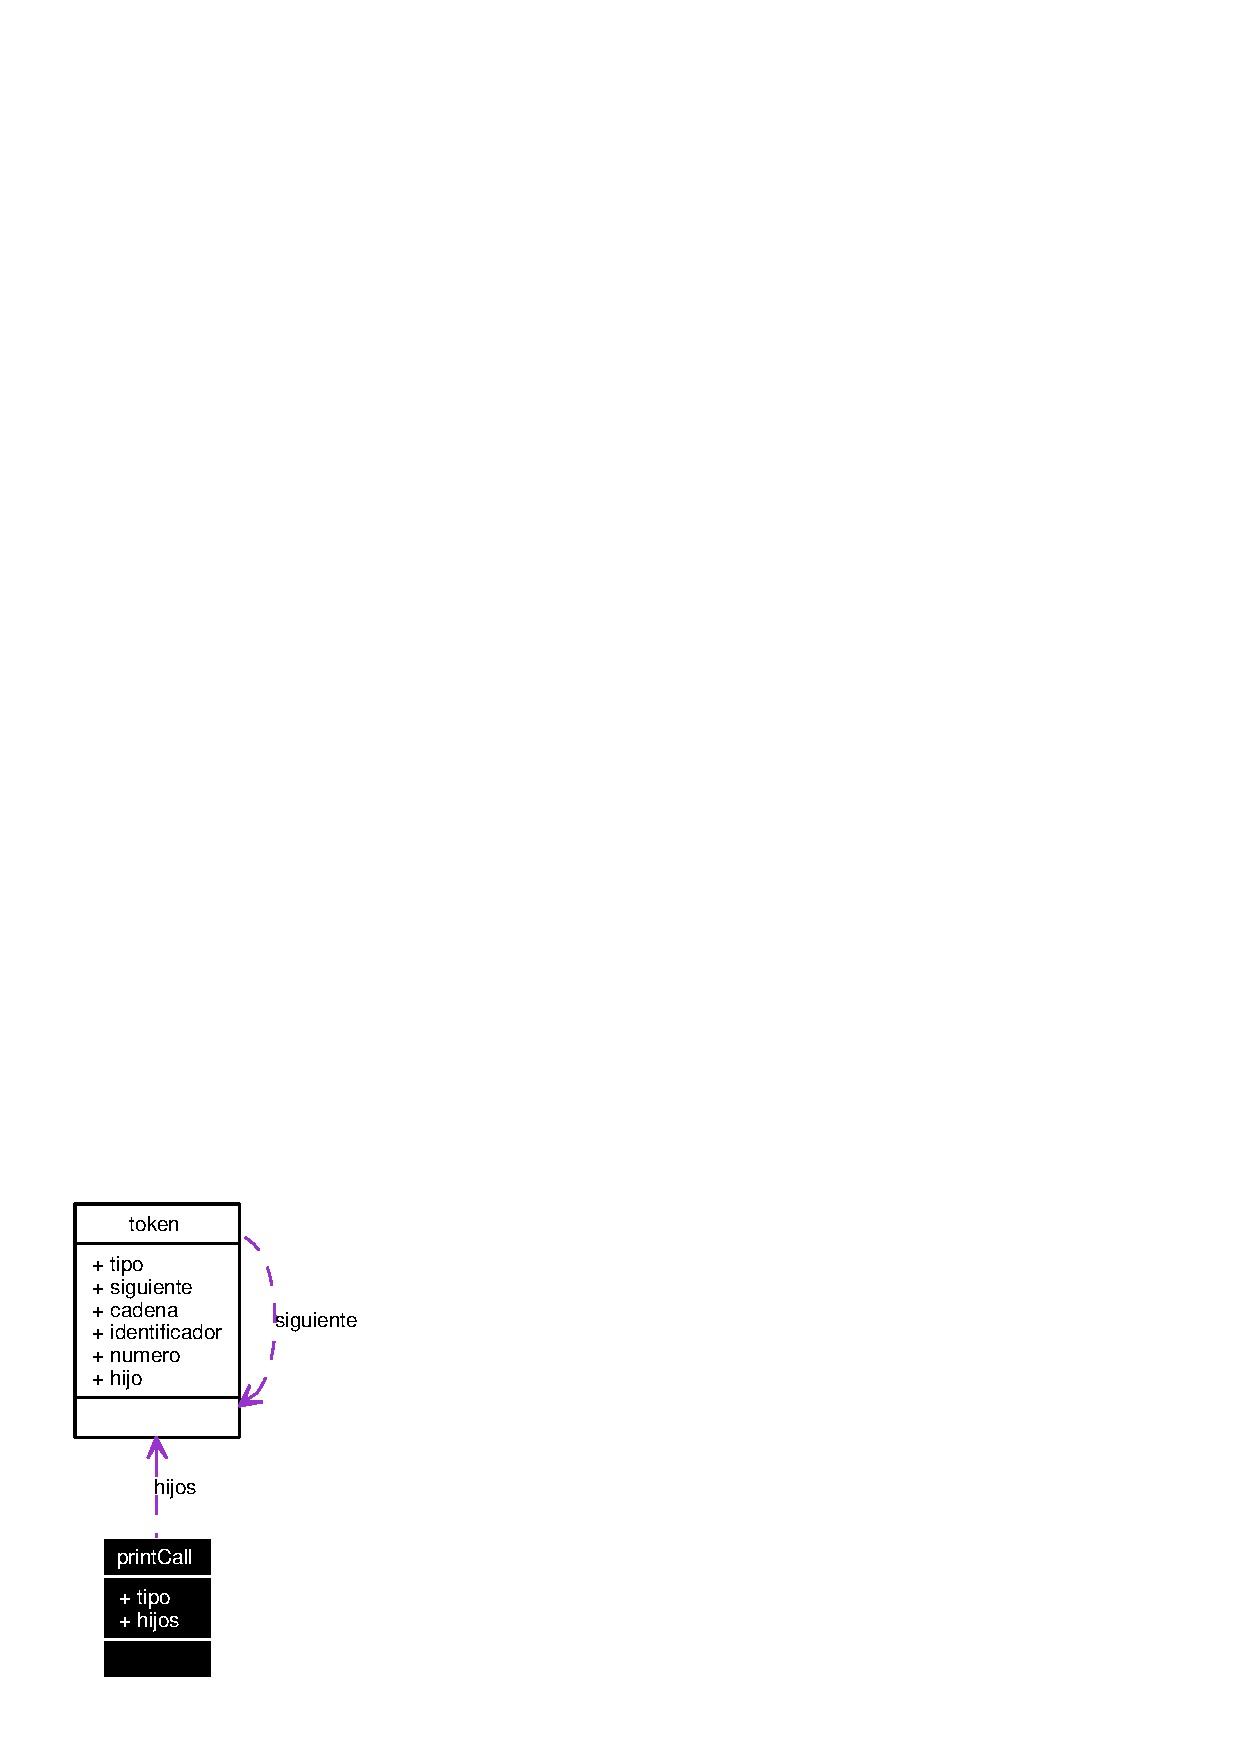
\includegraphics[width=86pt]{structprintCall__coll__graph}
\end{center}
\end{figure}
\subsection*{Atributos p\'{u}blicos}
\begin{CompactItemize}
\item 
int {\bf tipo}
\item 
{\bf token} $\ast$ {\bf hijos}
\begin{CompactList}\small\item\em Lista de tokens a imprimir. \item\end{CompactList}\end{CompactItemize}


\subsection{Descripci\'{o}n detallada}
Clase de almacenamiento de una llamada a Print o a vartablasimbolos en el AST. 



Definici\'{o}n en la l\'{\i}nea 221 del archivo ast.h.

\subsection{Documentaci\'{o}n de los datos miembro}
\index{printCall@{print\-Call}!hijos@{hijos}}
\index{hijos@{hijos}!printCall@{print\-Call}}
\subsubsection{\setlength{\rightskip}{0pt plus 5cm}{\bf token}$\ast$ {\bf print\-Call::hijos}}\label{structprintCall_o1}


Lista de tokens a imprimir. 



Definici\'{o}n en la l\'{\i}nea 223 del archivo ast.h.

Referenciado por borrar\-Print\-Call(), evaluar\-Print\-Call(), insertar\-Llamada(), y insertar\-Llamada\-Sym\-Tab().\index{printCall@{print\-Call}!tipo@{tipo}}
\index{tipo@{tipo}!printCall@{print\-Call}}
\subsubsection{\setlength{\rightskip}{0pt plus 5cm}int {\bf print\-Call::tipo}}\label{structprintCall_o0}




Definici\'{o}n en la l\'{\i}nea 222 del archivo ast.h.

Referenciado por evaluar\-Print\-Call(), insertar\-Llamada(), y insertar\-Llamada\-Sym\-Tab().

La documentaci\'{o}n para esta estructura fu\'{e} generada a partir del siguiente archivo:\begin{CompactItemize}
\item 
/media/docs/progra/c++/compiladores1/proy2/godzilla/src/{\bf ast.h}\end{CompactItemize}

\section{Referencia de la Estructura raiz}
\label{structraiz}\index{raiz@{raiz}}
punto de entrada del AST  


{\tt \#include $<$ast.h$>$}

Diagrama de colaboraci\'{o}n para raiz:\begin{figure}[H]
\begin{center}
\leavevmode
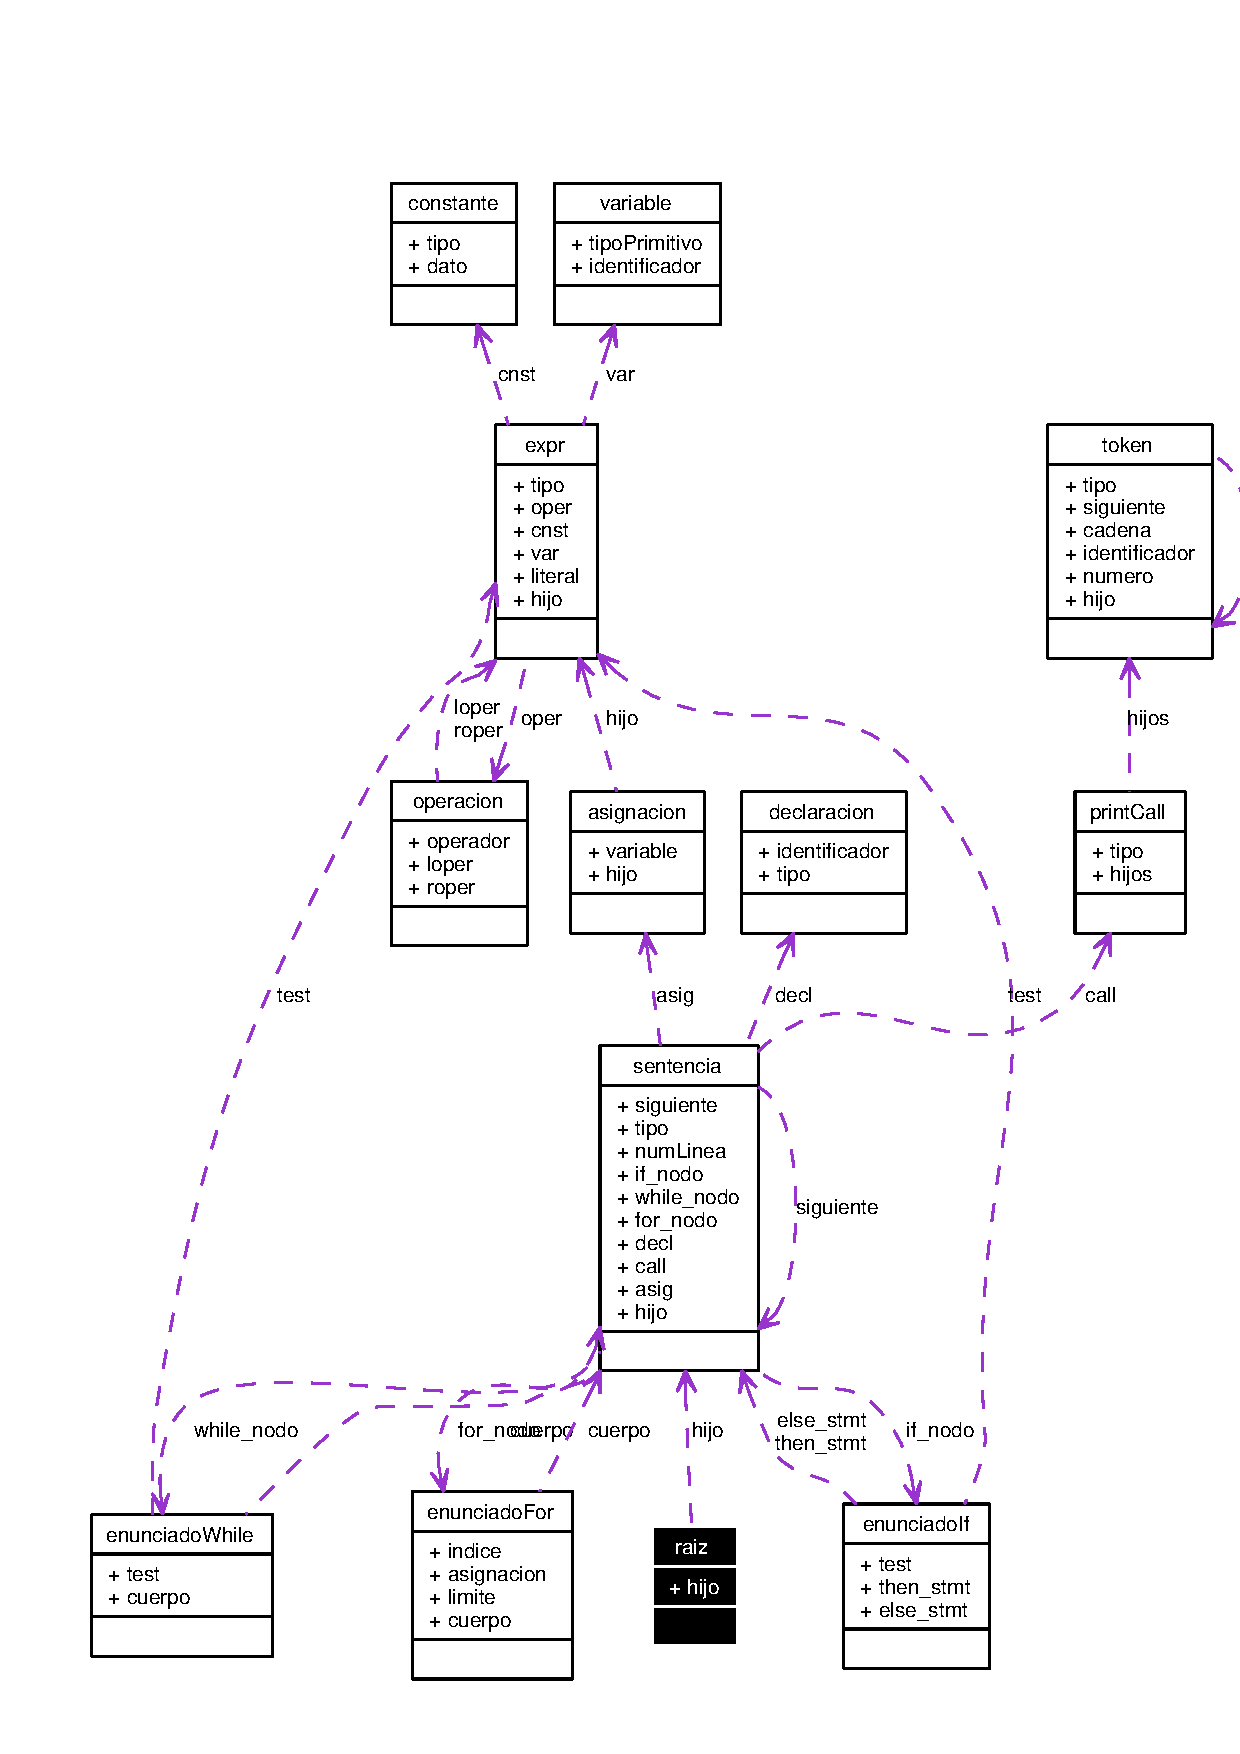
\includegraphics[width=320pt]{structraiz__coll__graph}
\end{center}
\end{figure}
\subsection*{Atributos p\'{u}blicos}
\begin{CompactItemize}
\item 
{\bf sentencia} $\ast$ {\bf hijo}
\begin{CompactList}\small\item\em Primer sentencia del arbol de sintaxis abstracto. \item\end{CompactList}\end{CompactItemize}


\subsection{Descripci\'{o}n detallada}
punto de entrada del AST 



Definici\'{o}n en la l\'{\i}nea 264 del archivo ast.h.

\subsection{Documentaci\'{o}n de los datos miembro}
\index{raiz@{raiz}!hijo@{hijo}}
\index{hijo@{hijo}!raiz@{raiz}}
\subsubsection{\setlength{\rightskip}{0pt plus 5cm}{\bf sentencia}$\ast$ {\bf raiz::hijo}}\label{structraiz_o0}


Primer sentencia del arbol de sintaxis abstracto. 



Definici\'{o}n en la l\'{\i}nea 265 del archivo ast.h.

Referenciado por borrar\-Arbol(), crear\-Raiz(), y recorrer\-Arbol().

La documentaci\'{o}n para esta estructura fu\'{e} generada a partir del siguiente archivo:\begin{CompactItemize}
\item 
/media/docs/progra/c++/compiladores1/proy2/godzilla/src/{\bf ast.h}\end{CompactItemize}

\section{Referencia de la Estructura sentencia}
\label{structsentencia}\index{sentencia@{sentencia}}
Clase de almacenamiento de raiz de un arbol de sentencias en el AST, siendo a su vez una lista.  


{\tt \#include $<$ast.h$>$}

Diagrama de colaboraci\'{o}n para sentencia:\begin{figure}[H]
\begin{center}
\leavevmode
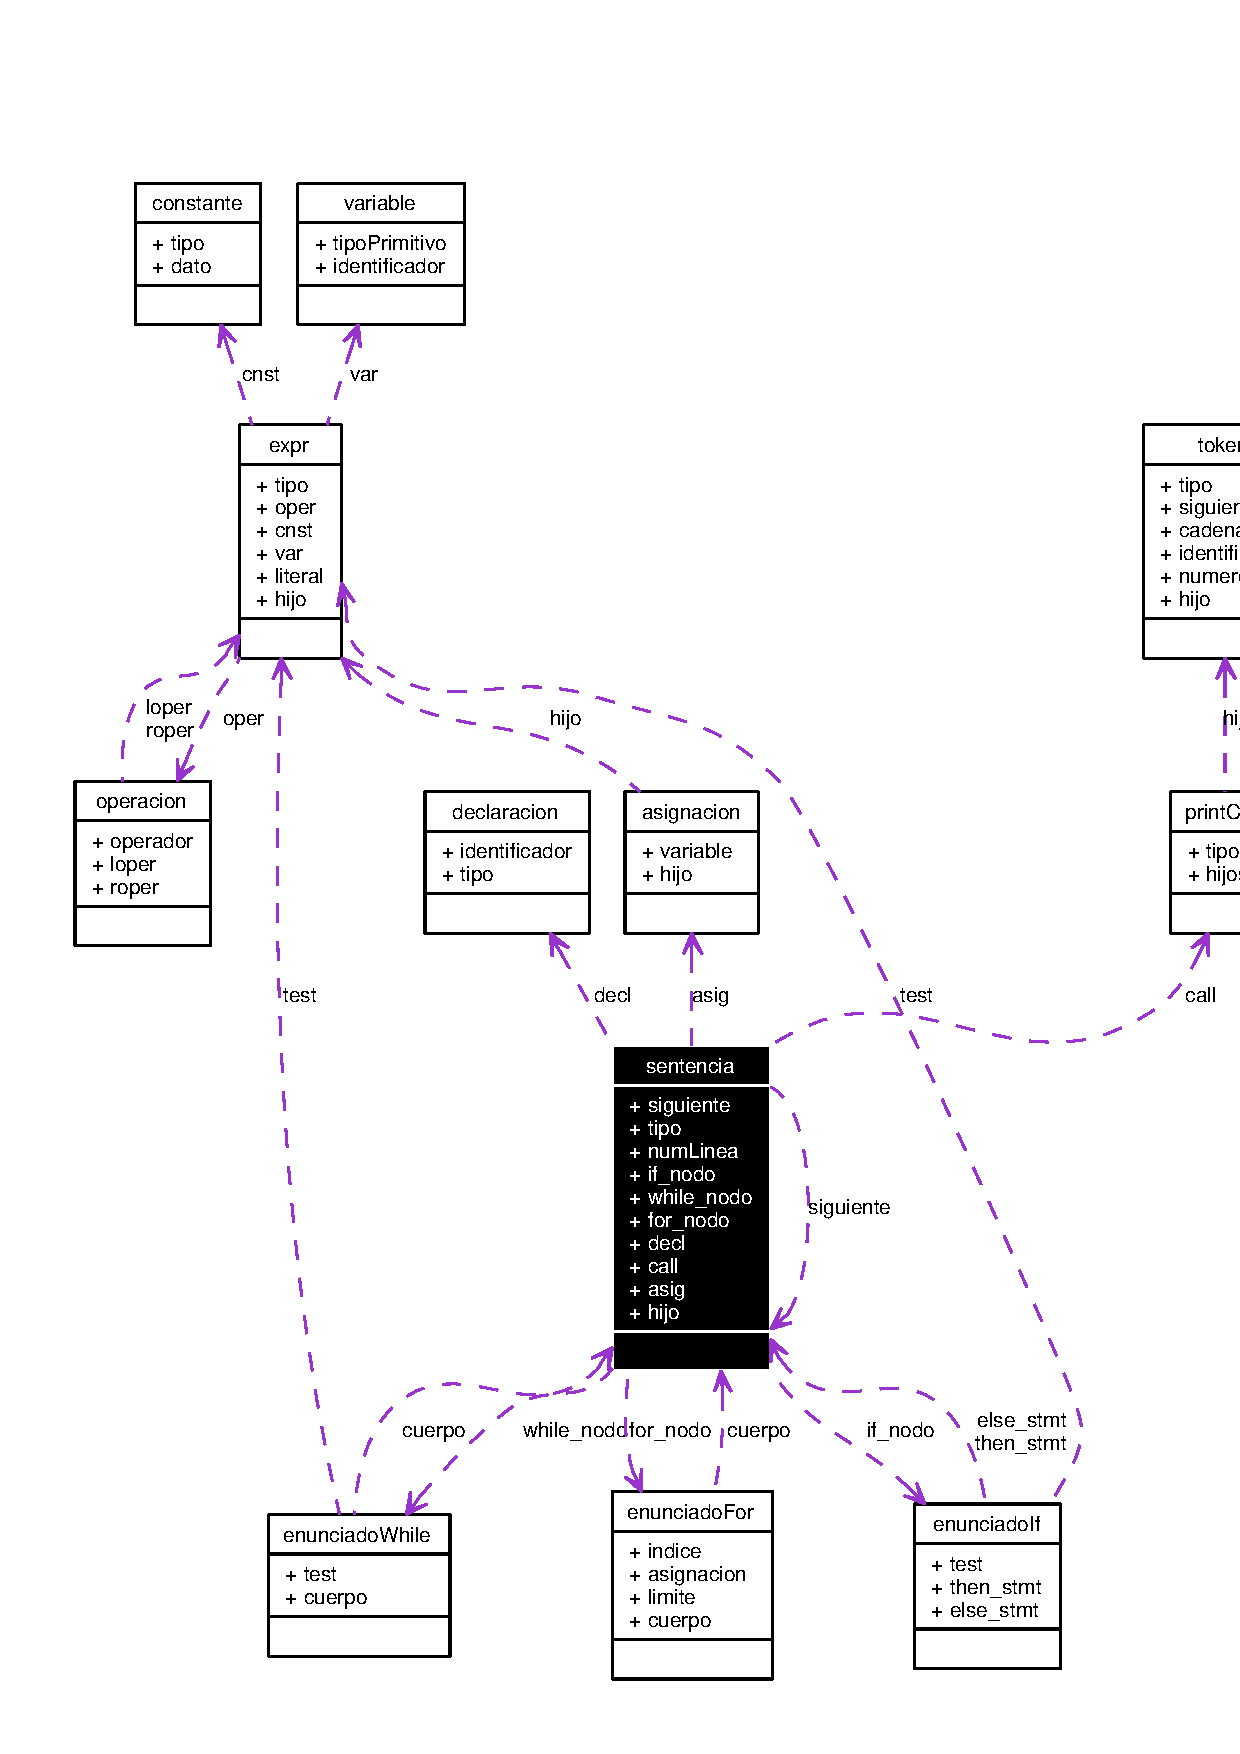
\includegraphics[width=343pt]{structsentencia__coll__graph}
\end{center}
\end{figure}
\subsection*{Atributos p\'{u}blicos}
\begin{CompactItemize}
\item 
{\bf sentencia} $\ast$ {\bf siguiente}
\begin{CompactList}\small\item\em Sentencia siguiente a evaluar. \item\end{CompactList}\item 
int {\bf tipo}
\begin{CompactList}\small\item\em Tipo de sentencia. \item\end{CompactList}\item 
int {\bf num\-Linea}
\begin{CompactList}\small\item\em Numero de linea en donde se encontraba la sentecia, esto es para escribir a archivo de error. \item\end{CompactList}\item 
\begin{tabbing}
xx\=xx\=xx\=xx\=xx\=xx\=xx\=xx\=xx\=\kill
union \{\\
\>{\bf enunciadoIf} $\ast$ {\bf if\_nodo}\\
\>{\bf enunciadoWhile} $\ast$ {\bf while\_nodo}\\
\>{\bf enunciadoFor} $\ast$ {\bf for\_nodo}\\
\>{\bf declaracion} $\ast$ {\bf decl}\\
\>{\bf printCall} $\ast$ {\bf call}\\
\>{\bf asignacion} $\ast$ {\bf asig}\\
\} {\bf hijo}\\

\end{tabbing}\begin{CompactList}\small\item\em Nodos hijos del arbol de sentencias. \item\end{CompactList}\end{CompactItemize}


\subsection{Descripci\'{o}n detallada}
Clase de almacenamiento de raiz de un arbol de sentencias en el AST, siendo a su vez una lista. 



Definici\'{o}n en la l\'{\i}nea 227 del archivo ast.h.

\subsection{Documentaci\'{o}n de los datos miembro}
\index{sentencia@{sentencia}!asig@{asig}}
\index{asig@{asig}!sentencia@{sentencia}}
\subsubsection{\setlength{\rightskip}{0pt plus 5cm}{\bf asignacion}$\ast$ {\bf sentencia::asig}}\label{structsentencia_o8}




Definici\'{o}n en la l\'{\i}nea 238 del archivo ast.h.\index{sentencia@{sentencia}!call@{call}}
\index{call@{call}!sentencia@{sentencia}}
\subsubsection{\setlength{\rightskip}{0pt plus 5cm}{\bf print\-Call}$\ast$ {\bf sentencia::call}}\label{structsentencia_o7}




Definici\'{o}n en la l\'{\i}nea 237 del archivo ast.h.\index{sentencia@{sentencia}!decl@{decl}}
\index{decl@{decl}!sentencia@{sentencia}}
\subsubsection{\setlength{\rightskip}{0pt plus 5cm}{\bf declaracion}$\ast$ {\bf sentencia::decl}}\label{structsentencia_o6}




Definici\'{o}n en la l\'{\i}nea 236 del archivo ast.h.\index{sentencia@{sentencia}!for_nodo@{for\_\-nodo}}
\index{for_nodo@{for\_\-nodo}!sentencia@{sentencia}}
\subsubsection{\setlength{\rightskip}{0pt plus 5cm}{\bf enunciado\-For}$\ast$ {\bf sentencia::for\_\-nodo}}\label{structsentencia_o5}




Definici\'{o}n en la l\'{\i}nea 235 del archivo ast.h.\index{sentencia@{sentencia}!hijo@{hijo}}
\index{hijo@{hijo}!sentencia@{sentencia}}
\subsubsection{\setlength{\rightskip}{0pt plus 5cm}union \{ ... \}  {\bf sentencia::hijo}}\label{structsentencia_o9}


Nodos hijos del arbol de sentencias. 



Referenciado por borrar\-Sentencias(), evaluar\-Sentencia(), y insertar\-Sentencia().\index{sentencia@{sentencia}!if_nodo@{if\_\-nodo}}
\index{if_nodo@{if\_\-nodo}!sentencia@{sentencia}}
\subsubsection{\setlength{\rightskip}{0pt plus 5cm}{\bf enunciado\-If}$\ast$ {\bf sentencia::if\_\-nodo}}\label{structsentencia_o3}




Definici\'{o}n en la l\'{\i}nea 233 del archivo ast.h.\index{sentencia@{sentencia}!numLinea@{numLinea}}
\index{numLinea@{numLinea}!sentencia@{sentencia}}
\subsubsection{\setlength{\rightskip}{0pt plus 5cm}int {\bf sentencia::num\-Linea}}\label{structsentencia_o2}


Numero de linea en donde se encontraba la sentecia, esto es para escribir a archivo de error. 



Definici\'{o}n en la l\'{\i}nea 230 del archivo ast.h.

Referenciado por error(), y insertar\-Sentencia().\index{sentencia@{sentencia}!siguiente@{siguiente}}
\index{siguiente@{siguiente}!sentencia@{sentencia}}
\subsubsection{\setlength{\rightskip}{0pt plus 5cm}{\bf sentencia}$\ast$ {\bf sentencia::siguiente}}\label{structsentencia_o0}


Sentencia siguiente a evaluar. 



Definici\'{o}n en la l\'{\i}nea 228 del archivo ast.h.

Referenciado por borrar\-Sentencias(), concatenar\-Sentencia(), insertar\-Sentencia(), y recorrer\-Sentencia().\index{sentencia@{sentencia}!tipo@{tipo}}
\index{tipo@{tipo}!sentencia@{sentencia}}
\subsubsection{\setlength{\rightskip}{0pt plus 5cm}int {\bf sentencia::tipo}}\label{structsentencia_o1}


Tipo de sentencia. 



Definici\'{o}n en la l\'{\i}nea 229 del archivo ast.h.

Referenciado por borrar\-Sentencias(), evaluar\-Sentencia(), y insertar\-Sentencia().\index{sentencia@{sentencia}!while_nodo@{while\_\-nodo}}
\index{while_nodo@{while\_\-nodo}!sentencia@{sentencia}}
\subsubsection{\setlength{\rightskip}{0pt plus 5cm}{\bf enunciado\-While}$\ast$ {\bf sentencia::while\_\-nodo}}\label{structsentencia_o4}




Definici\'{o}n en la l\'{\i}nea 234 del archivo ast.h.

La documentaci\'{o}n para esta estructura fu\'{e} generada a partir del siguiente archivo:\begin{CompactItemize}
\item 
/media/docs/progra/c++/compiladores1/proy2/godzilla/src/{\bf ast.h}\end{CompactItemize}

\section{Referencia de la Estructura symbol}
\label{structsymbol}\index{symbol@{symbol}}
Nodo de la tabla de simbolos.  


{\tt \#include $<$symtab.h$>$}

Diagrama de colaboraci\'{o}n para symbol:\begin{figure}[H]
\begin{center}
\leavevmode
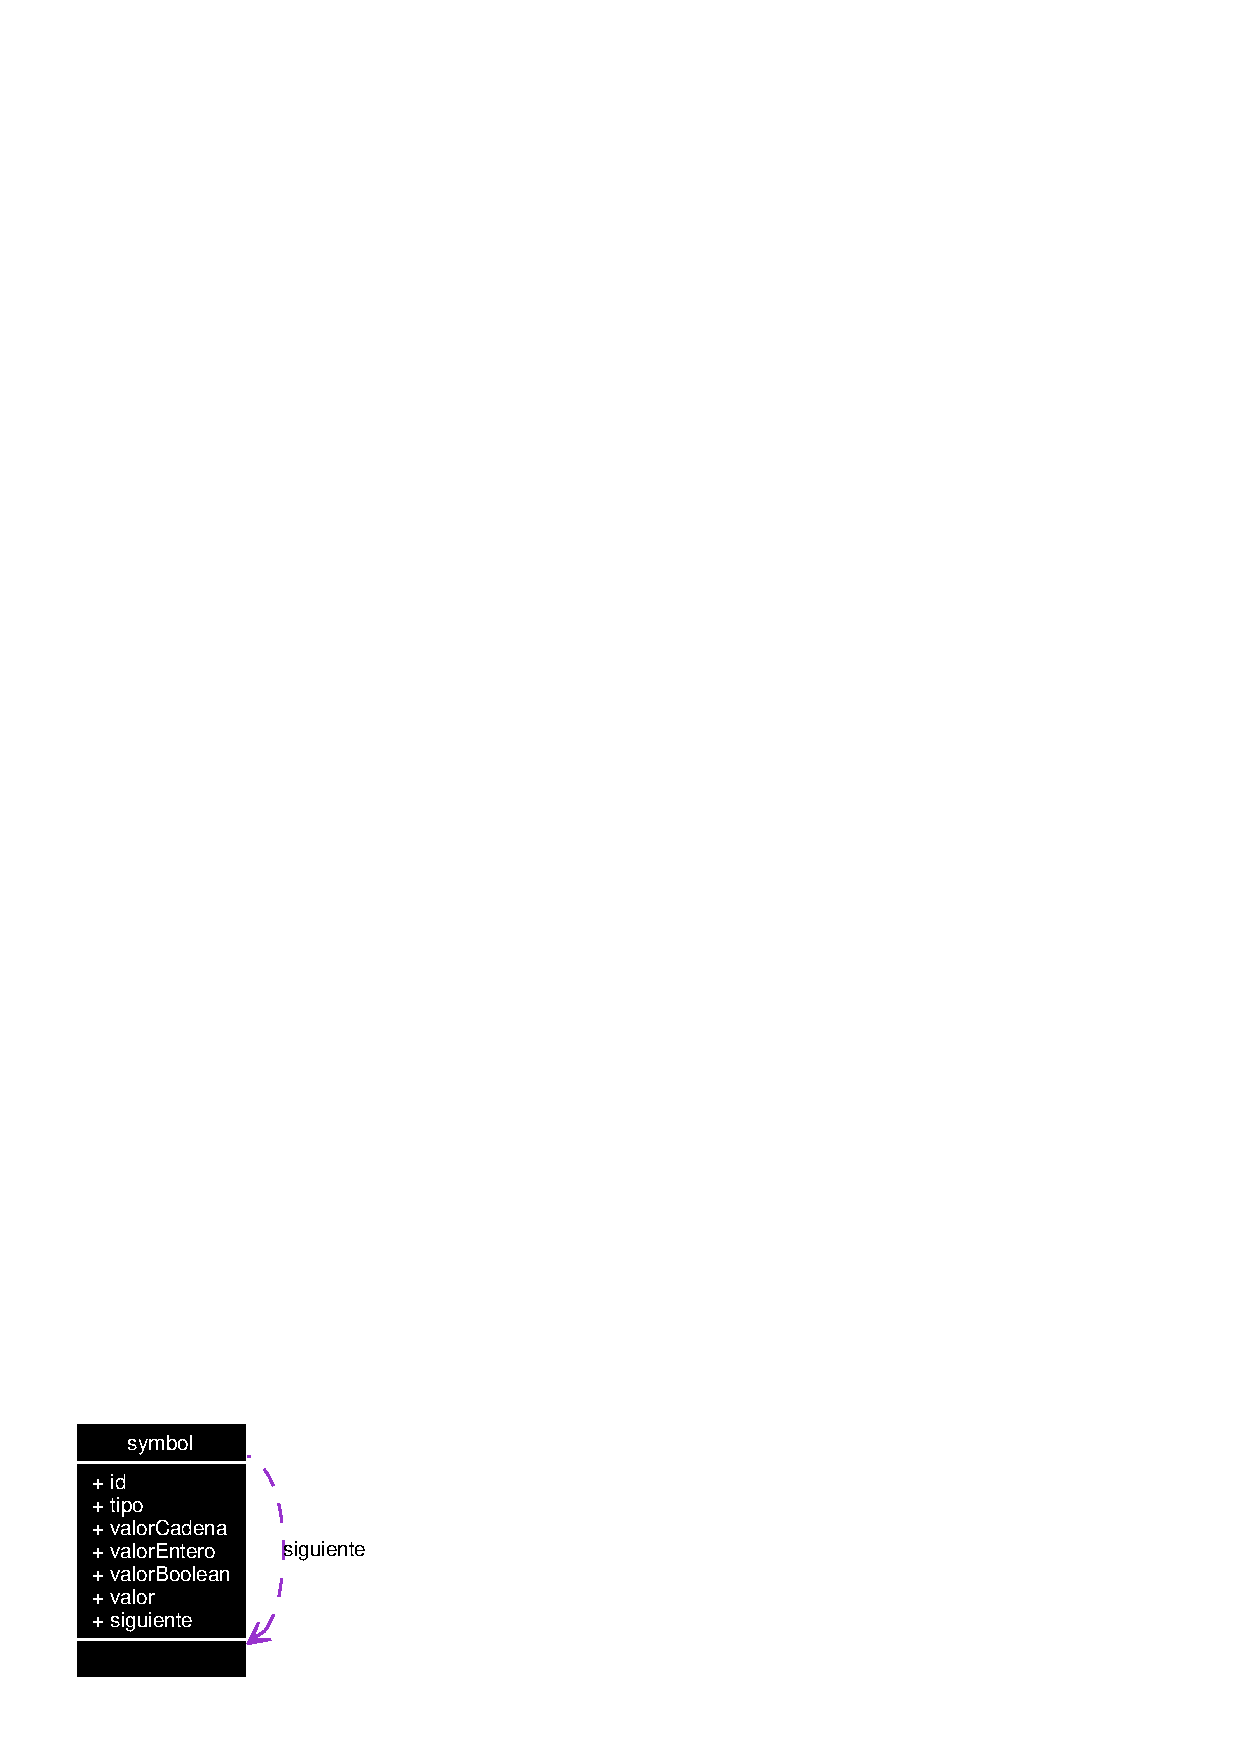
\includegraphics[width=88pt]{structsymbol__coll__graph}
\end{center}
\end{figure}
\subsection*{Atributos p\'{u}blicos}
\begin{CompactItemize}
\item 
char $\ast$ {\bf id}
\item 
int {\bf tipo}
\item 
\begin{tabbing}
xx\=xx\=xx\=xx\=xx\=xx\=xx\=xx\=xx\=\kill
union \{\\
\>char $\ast$ {\bf valorCadena}\\
\>int {\bf valorEntero}\\
\>char {\bf valorBoolean}\\
\} {\bf valor}\\

\end{tabbing}\item 
{\bf symbol} $\ast$ {\bf siguiente}
\end{CompactItemize}


\subsection{Descripci\'{o}n detallada}
Nodo de la tabla de simbolos. 



Definici\'{o}n en la l\'{\i}nea 13 del archivo symtab.h.

\subsection{Documentaci\'{o}n de los datos miembro}
\index{symbol@{symbol}!id@{id}}
\index{id@{id}!symbol@{symbol}}
\subsubsection{\setlength{\rightskip}{0pt plus 5cm}char$\ast$ {\bf symbol::id}}\label{structsymbol_o0}




Definici\'{o}n en la l\'{\i}nea 14 del archivo symtab.h.

Referenciado por borrar\-Nodos(), insertar\-Simbolo(), y print\-Symtab\-File().\index{symbol@{symbol}!siguiente@{siguiente}}
\index{siguiente@{siguiente}!symbol@{symbol}}
\subsubsection{\setlength{\rightskip}{0pt plus 5cm}{\bf symbol}$\ast$ {\bf symbol::siguiente}}\label{structsymbol_o6}




Definici\'{o}n en la l\'{\i}nea 21 del archivo symtab.h.

Referenciado por borrar\-Nodos(), buscar\-Simbolo(), insertar\-Simbolo(), y print\-Symtab\-File().\index{symbol@{symbol}!tipo@{tipo}}
\index{tipo@{tipo}!symbol@{symbol}}
\subsubsection{\setlength{\rightskip}{0pt plus 5cm}int {\bf symbol::tipo}}\label{structsymbol_o1}




Definici\'{o}n en la l\'{\i}nea 15 del archivo symtab.h.

Referenciado por borrar\-Nodos(), evaluar\-Asignacion(), evaluar\-Expresion(), evaluar\-For(), imprimir\-Tokens(), insertar\-Simbolo(), y print\-Symtab\-File().\index{symbol@{symbol}!valor@{valor}}
\index{valor@{valor}!symbol@{symbol}}
\subsubsection{\setlength{\rightskip}{0pt plus 5cm}union \{ ... \}  {\bf symbol::valor}}\label{structsymbol_o5}




Referenciado por borrar\-Nodos(), evaluar\-Asignacion(), evaluar\-Expresion(), evaluar\-For(), imprimir\-Tokens(), insertar\-Simbolo(), y print\-Symtab\-File().\index{symbol@{symbol}!valorBoolean@{valorBoolean}}
\index{valorBoolean@{valorBoolean}!symbol@{symbol}}
\subsubsection{\setlength{\rightskip}{0pt plus 5cm}char {\bf symbol::valor\-Boolean}}\label{structsymbol_o4}




Definici\'{o}n en la l\'{\i}nea 19 del archivo symtab.h.\index{symbol@{symbol}!valorCadena@{valorCadena}}
\index{valorCadena@{valorCadena}!symbol@{symbol}}
\subsubsection{\setlength{\rightskip}{0pt plus 5cm}char$\ast$ {\bf symbol::valor\-Cadena}}\label{structsymbol_o2}




Definici\'{o}n en la l\'{\i}nea 17 del archivo symtab.h.\index{symbol@{symbol}!valorEntero@{valorEntero}}
\index{valorEntero@{valorEntero}!symbol@{symbol}}
\subsubsection{\setlength{\rightskip}{0pt plus 5cm}int {\bf symbol::valor\-Entero}}\label{structsymbol_o3}




Definici\'{o}n en la l\'{\i}nea 18 del archivo symtab.h.

La documentaci\'{o}n para esta estructura fu\'{e} generada a partir del siguiente archivo:\begin{CompactItemize}
\item 
/media/docs/progra/c++/compiladores1/proy2/godzilla/src/{\bf symtab.h}\end{CompactItemize}

\section{Referencia de la Estructura symtab}
\label{structsymtab}\index{symtab@{symtab}}
Tabla de simbolos usando modelo de lista simple.  


{\tt \#include $<$symtab.h$>$}

Diagrama de colaboraci\'{o}n para symtab:\begin{figure}[H]
\begin{center}
\leavevmode
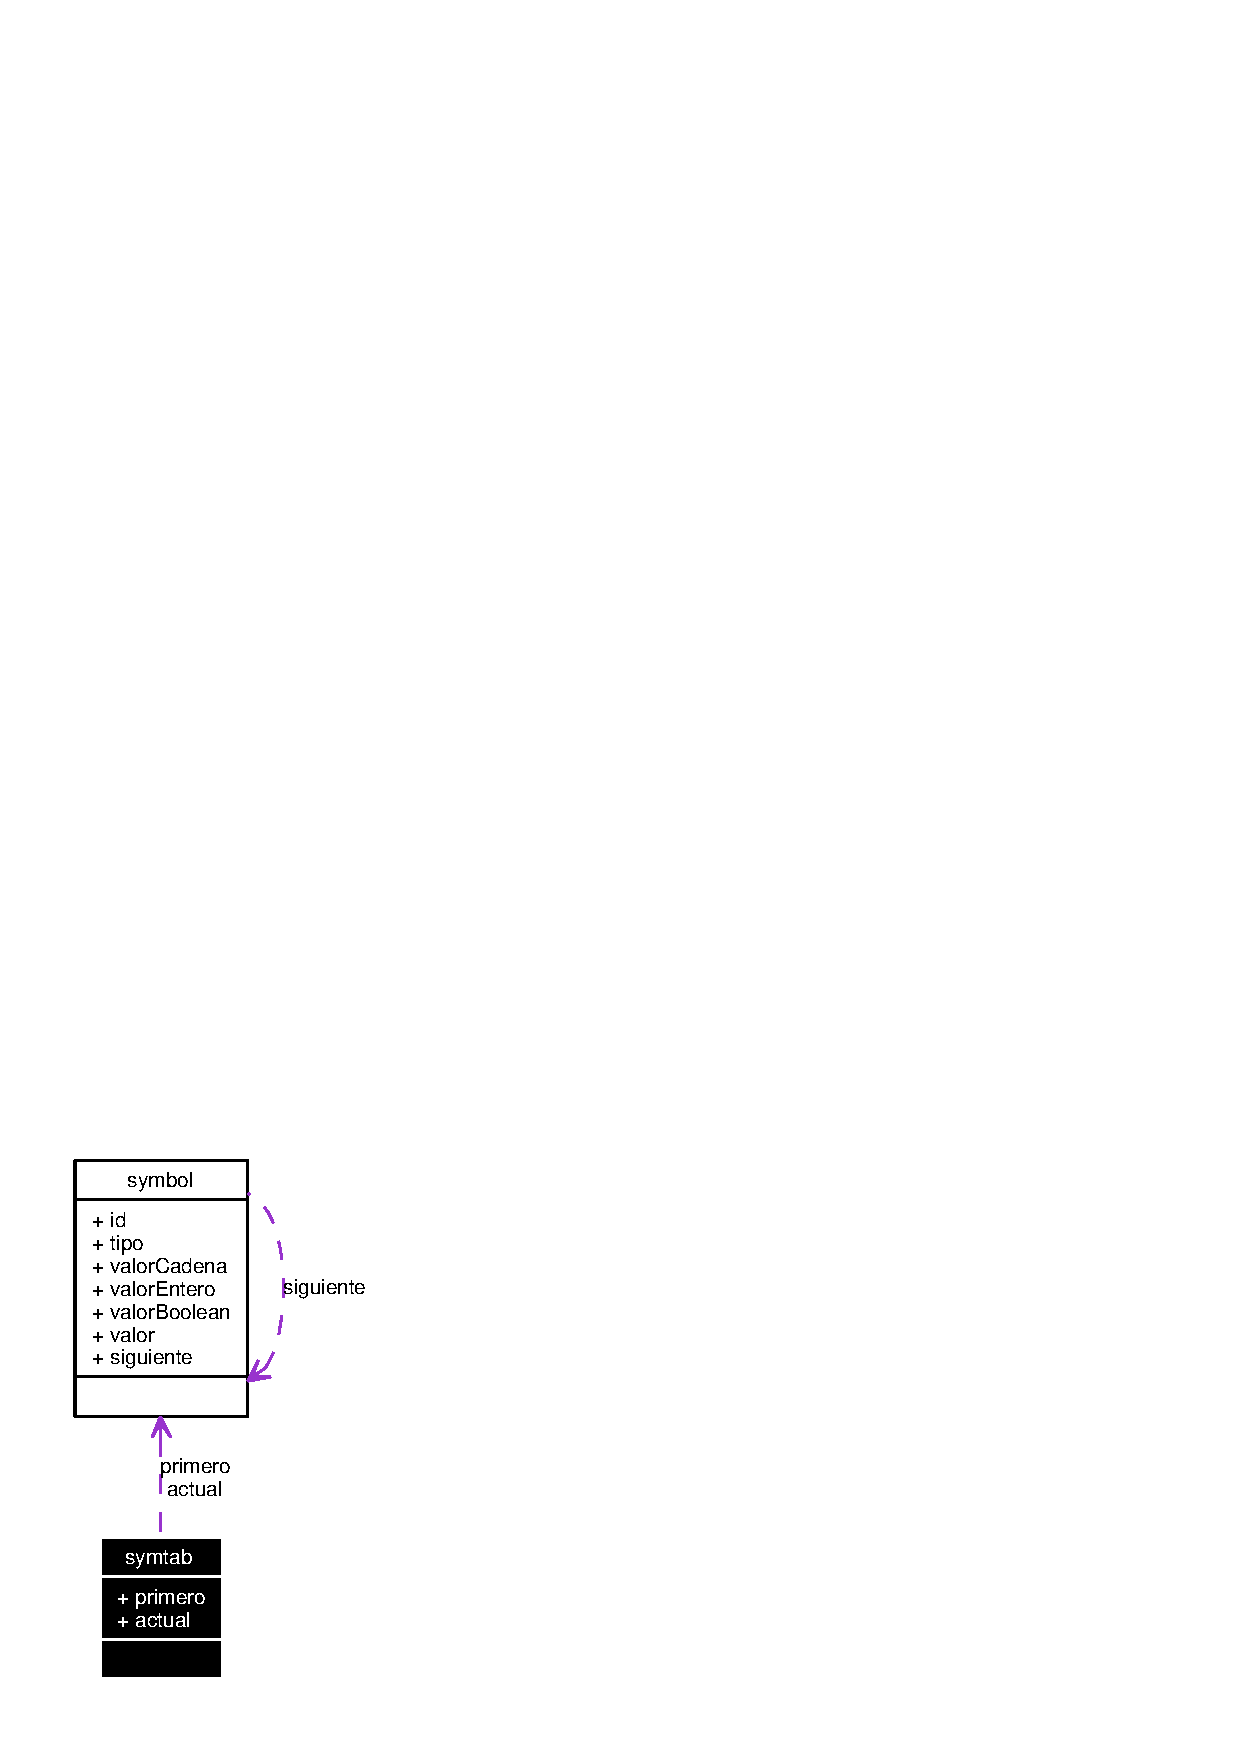
\includegraphics[width=88pt]{structsymtab__coll__graph}
\end{center}
\end{figure}
\subsection*{Atributos p\'{u}blicos}
\begin{CompactItemize}
\item 
{\bf symbol} $\ast$ {\bf primero}
\item 
{\bf symbol} $\ast$ {\bf actual}
\end{CompactItemize}


\subsection{Descripci\'{o}n detallada}
Tabla de simbolos usando modelo de lista simple. 



Definici\'{o}n en la l\'{\i}nea 24 del archivo symtab.h.

\subsection{Documentaci\'{o}n de los datos miembro}
\index{symtab@{symtab}!actual@{actual}}
\index{actual@{actual}!symtab@{symtab}}
\subsubsection{\setlength{\rightskip}{0pt plus 5cm}{\bf symbol}$\ast$ {\bf symtab::actual}}\label{structsymtab_o1}




Definici\'{o}n en la l\'{\i}nea 26 del archivo symtab.h.

Referenciado por borrar\-Tabla(), buscar\-Simbolo(), insertar\-Simbolo(), y print\-Symtab\-File().\index{symtab@{symtab}!primero@{primero}}
\index{primero@{primero}!symtab@{symtab}}
\subsubsection{\setlength{\rightskip}{0pt plus 5cm}{\bf symbol}$\ast$ {\bf symtab::primero}}\label{structsymtab_o0}




Definici\'{o}n en la l\'{\i}nea 25 del archivo symtab.h.

Referenciado por borrar\-Tabla(), buscar\-Simbolo(), insertar\-Simbolo(), y print\-Symtab\-File().

La documentaci\'{o}n para esta estructura fu\'{e} generada a partir del siguiente archivo:\begin{CompactItemize}
\item 
/media/docs/progra/c++/compiladores1/proy2/godzilla/src/{\bf symtab.h}\end{CompactItemize}

\section{Referencia de la Estructura tipo\-Error}
\label{structtipoError}\index{tipoError@{tipoError}}
Clase de almacenamiento de error.  


{\tt \#include $<$colaerr.h$>$}

\subsection*{Atributos p\'{u}blicos}
\begin{CompactItemize}
\item 
int {\bf linea}
\item 
int {\bf col}
\item 
char $\ast$ {\bf desc}
\end{CompactItemize}


\subsection{Descripci\'{o}n detallada}
Clase de almacenamiento de error. 



Definici\'{o}n en la l\'{\i}nea 28 del archivo colaerr.h.

\subsection{Documentaci\'{o}n de los datos miembro}
\index{tipoError@{tipo\-Error}!col@{col}}
\index{col@{col}!tipoError@{tipo\-Error}}
\subsubsection{\setlength{\rightskip}{0pt plus 5cm}int {\bf tipo\-Error::col}}\label{structtipoError_o1}




Definici\'{o}n en la l\'{\i}nea 30 del archivo colaerr.h.

Referenciado por error\-Lexico(), error\-Semantico(), error\-Sintactico(), y escribir\-Error\-Log\-XML().\index{tipoError@{tipo\-Error}!desc@{desc}}
\index{desc@{desc}!tipoError@{tipo\-Error}}
\subsubsection{\setlength{\rightskip}{0pt plus 5cm}char$\ast$ {\bf tipo\-Error::desc}}\label{structtipoError_o2}




Definici\'{o}n en la l\'{\i}nea 31 del archivo colaerr.h.

Referenciado por error\-Lexico(), error\-Semantico(), error\-Sintactico(), y escribir\-Error\-Log\-XML().\index{tipoError@{tipo\-Error}!linea@{linea}}
\index{linea@{linea}!tipoError@{tipo\-Error}}
\subsubsection{\setlength{\rightskip}{0pt plus 5cm}int {\bf tipo\-Error::linea}}\label{structtipoError_o0}




Definici\'{o}n en la l\'{\i}nea 29 del archivo colaerr.h.

Referenciado por error\-Lexico(), error\-Semantico(), error\-Sintactico(), y escribir\-Error\-Log\-XML().

La documentaci\'{o}n para esta estructura fu\'{e} generada a partir del siguiente archivo:\begin{CompactItemize}
\item 
/media/docs/progra/c++/compiladores1/proy2/godzilla/src/{\bf colaerr.h}\end{CompactItemize}

\section{Referencia de la Estructura token}
\label{structtoken}\index{token@{token}}
Clase de almacenamiento de raiz de una lista enlazada de Tokens a imprimir con el comando Print en el AST.  


{\tt \#include $<$ast.h$>$}

Diagrama de colaboraci\'{o}n para token:\begin{figure}[H]
\begin{center}
\leavevmode
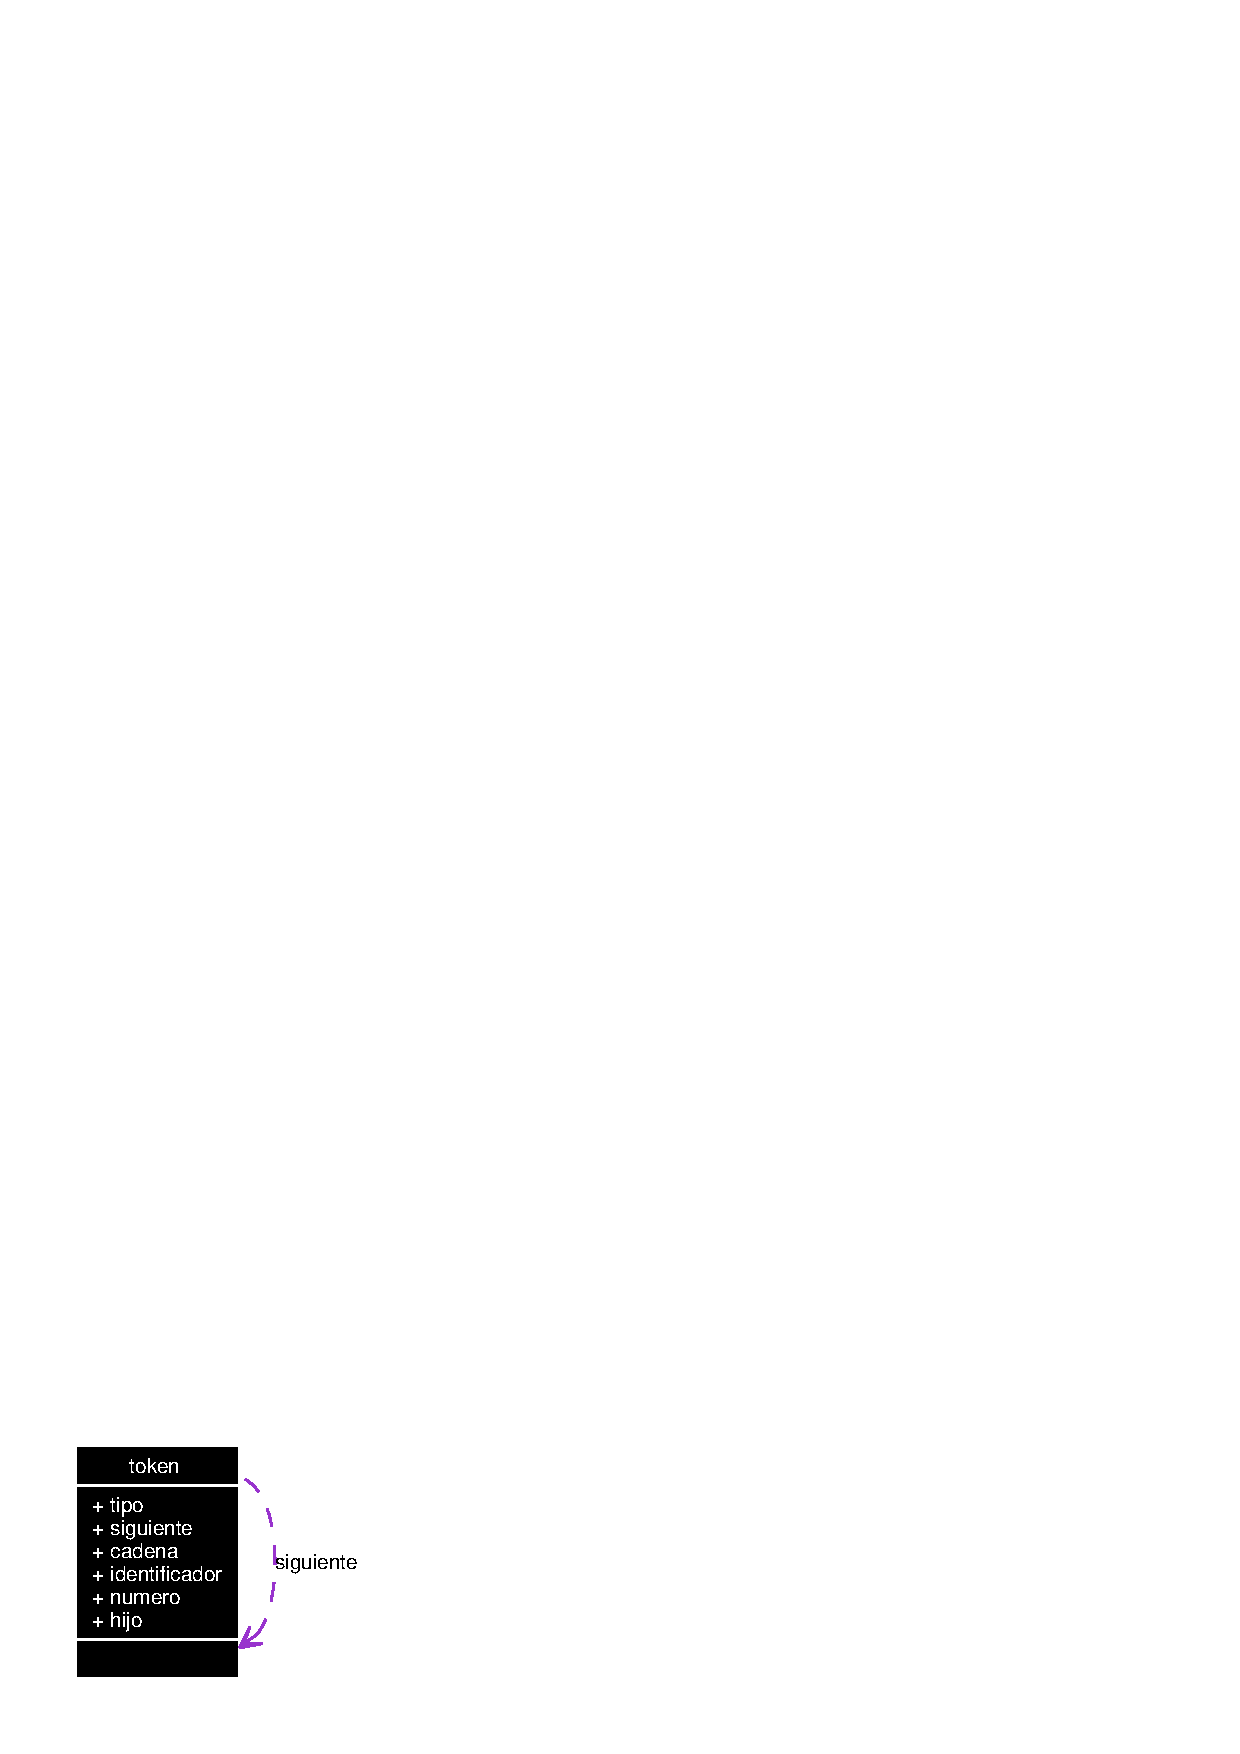
\includegraphics[width=86pt]{structtoken__coll__graph}
\end{center}
\end{figure}
\subsection*{Atributos p\'{u}blicos}
\begin{CompactItemize}
\item 
int {\bf tipo}
\begin{CompactList}\small\item\em Tipo de token a evaluar. \item\end{CompactList}\item 
{\bf token} $\ast$ {\bf siguiente}
\begin{CompactList}\small\item\em puntero a token siguiente en la lista \item\end{CompactList}\item 
\begin{tabbing}
xx\=xx\=xx\=xx\=xx\=xx\=xx\=xx\=xx\=\kill
union \{\\
\>char $\ast$ {\bf cadena}\\
\>char $\ast$ {\bf identificador}\\
\>int {\bf numero}\\
\} {\bf hijo}\\

\end{tabbing}\begin{CompactList}\small\item\em puntero a token \item\end{CompactList}\end{CompactItemize}


\subsection{Descripci\'{o}n detallada}
Clase de almacenamiento de raiz de una lista enlazada de Tokens a imprimir con el comando Print en el AST. 



Definici\'{o}n en la l\'{\i}nea 243 del archivo ast.h.

\subsection{Documentaci\'{o}n de los datos miembro}
\index{token@{token}!cadena@{cadena}}
\index{cadena@{cadena}!token@{token}}
\subsubsection{\setlength{\rightskip}{0pt plus 5cm}char$\ast$ {\bf token::cadena}}\label{structtoken_o2}




Definici\'{o}n en la l\'{\i}nea 247 del archivo ast.h.\index{token@{token}!hijo@{hijo}}
\index{hijo@{hijo}!token@{token}}
\subsubsection{\setlength{\rightskip}{0pt plus 5cm}union \{ ... \}  {\bf token::hijo}}\label{structtoken_o5}


puntero a token 



Referenciado por borrar\-Tokens(), imprimir\-Tokens(), y insertar\-Token().\index{token@{token}!identificador@{identificador}}
\index{identificador@{identificador}!token@{token}}
\subsubsection{\setlength{\rightskip}{0pt plus 5cm}char$\ast$ {\bf token::identificador}}\label{structtoken_o3}




Definici\'{o}n en la l\'{\i}nea 248 del archivo ast.h.\index{token@{token}!numero@{numero}}
\index{numero@{numero}!token@{token}}
\subsubsection{\setlength{\rightskip}{0pt plus 5cm}int {\bf token::numero}}\label{structtoken_o4}




Definici\'{o}n en la l\'{\i}nea 249 del archivo ast.h.\index{token@{token}!siguiente@{siguiente}}
\index{siguiente@{siguiente}!token@{token}}
\subsubsection{\setlength{\rightskip}{0pt plus 5cm}{\bf token}$\ast$ {\bf token::siguiente}}\label{structtoken_o1}


puntero a token siguiente en la lista 



Definici\'{o}n en la l\'{\i}nea 245 del archivo ast.h.

Referenciado por borrar\-Tokens(), concatenar\-Tokens(), imprimir\-Tokens(), y insertar\-Token().\index{token@{token}!tipo@{tipo}}
\index{tipo@{tipo}!token@{token}}
\subsubsection{\setlength{\rightskip}{0pt plus 5cm}int {\bf token::tipo}}\label{structtoken_o0}


Tipo de token a evaluar. 



Definici\'{o}n en la l\'{\i}nea 244 del archivo ast.h.

Referenciado por borrar\-Tokens(), imprimir\-Tokens(), y insertar\-Token().

La documentaci\'{o}n para esta estructura fu\'{e} generada a partir del siguiente archivo:\begin{CompactItemize}
\item 
/media/docs/progra/c++/compiladores1/proy2/godzilla/src/{\bf ast.h}\end{CompactItemize}

\section{Referencia de la Estructura variable}
\label{structvariable}\index{variable@{variable}}
Clase de almacenamiento de variables en el AST.  


{\tt \#include $<$ast.h$>$}

\subsection*{Atributos p\'{u}blicos}
\begin{CompactItemize}
\item 
int {\bf tipo\-Primitivo}
\begin{CompactList}\small\item\em Tipo de dato. \item\end{CompactList}\item 
char $\ast$ {\bf identificador}
\begin{CompactList}\small\item\em identificador \item\end{CompactList}\end{CompactItemize}


\subsection{Descripci\'{o}n detallada}
Clase de almacenamiento de variables en el AST. 



Definici\'{o}n en la l\'{\i}nea 169 del archivo ast.h.

\subsection{Documentaci\'{o}n de los datos miembro}
\index{variable@{variable}!identificador@{identificador}}
\index{identificador@{identificador}!variable@{variable}}
\subsubsection{\setlength{\rightskip}{0pt plus 5cm}char$\ast$ {\bf variable::identificador}}\label{structvariable_o1}


identificador 



Definici\'{o}n en la l\'{\i}nea 171 del archivo ast.h.

Referenciado por insertar\-Variable().\index{variable@{variable}!tipoPrimitivo@{tipoPrimitivo}}
\index{tipoPrimitivo@{tipoPrimitivo}!variable@{variable}}
\subsubsection{\setlength{\rightskip}{0pt plus 5cm}int {\bf variable::tipo\-Primitivo}}\label{structvariable_o0}


Tipo de dato. 



Definici\'{o}n en la l\'{\i}nea 170 del archivo ast.h.

La documentaci\'{o}n para esta estructura fu\'{e} generada a partir del siguiente archivo:\begin{CompactItemize}
\item 
/media/docs/progra/c++/compiladores1/proy2/godzilla/src/{\bf ast.h}\end{CompactItemize}

\chapter{godzilla Documentaci\'{o}n de archivos}
\section{Referencia del Archivo /media/docs/progra/c++/compiladores1/proy2/godzilla/src/ast.c}
\label{ast_8c}\index{/media/docs/progra/c++/compiladores1/proy2/godzilla/src/ast.c@{/media/docs/progra/c++/compiladores1/proy2/godzilla/src/ast.c}}
Implementacion del arbol de sintaxis abstracta. 

{\tt \#include $<$stdio.h$>$}\par
{\tt \#include $<$stdlib.h$>$}\par
{\tt \#include $<$string.h$>$}\par
{\tt \#include \char`\"{}ast.h\char`\"{}}\par


Dependencia gr\'{a}fica adjunta para ast.c:\begin{figure}[H]
\begin{center}
\leavevmode
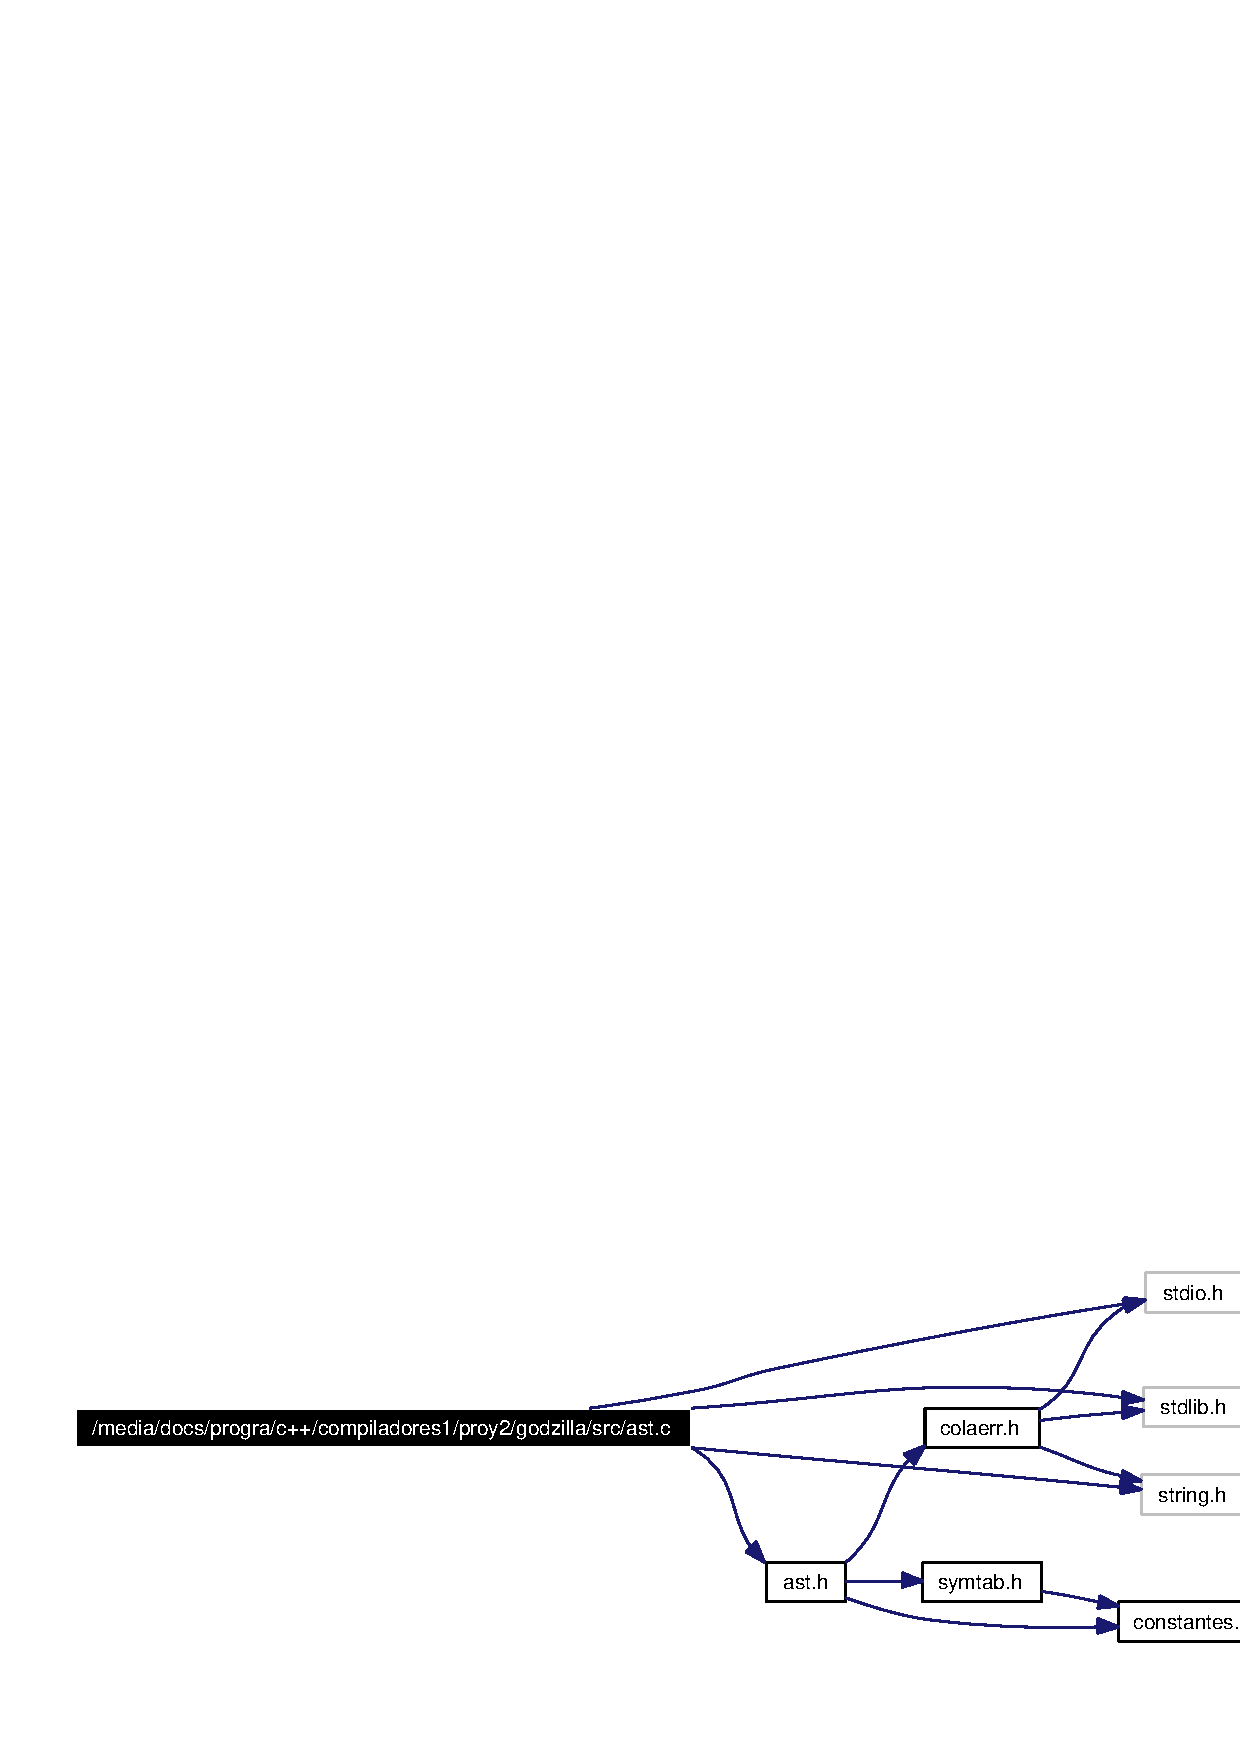
\includegraphics[width=305pt]{ast_8c__incl}
\end{center}
\end{figure}
\subsection*{Funciones}
\begin{CompactItemize}
\item 
{\bf nodo} $\ast$ {\bf ref\-Nodo\-Hijo} (int tipo, void $\ast$dato)
\begin{CompactList}\small\item\em Crea un nodo que refiere al nodo recien creado para sea utilizado por el nodo anterior a este. \item\end{CompactList}\item 
{\bf nodo} $\ast$ {\bf insertar\-Constante} (int tipo, int dato)
\begin{CompactList}\small\item\em Agrega una constante al arbol de expresiones. \item\end{CompactList}\item 
{\bf nodo} $\ast$ {\bf insertar\-Variable} (char $\ast$ident)
\begin{CompactList}\small\item\em Agrega una variable al arbol de expresiones. \item\end{CompactList}\item 
{\bf nodo} $\ast$ {\bf insertar\-Cadena} (char $\ast$cadena)
\begin{CompactList}\small\item\em Agrega una cadena al arbol de expresiones. \item\end{CompactList}\item 
{\bf nodo} $\ast$ {\bf insertar\-Operacion} (int operador, {\bf nodo} $\ast$l, {\bf nodo} $\ast$r)
\begin{CompactList}\small\item\em Inserta una operacion al arbol de expresiones. \item\end{CompactList}\item 
{\bf nodo} $\ast$ {\bf insertar\-Expresion} ({\bf nodo} $\ast$n)
\begin{CompactList}\small\item\em Agrega un nuevo arbol de expresiones al arbol principal. \item\end{CompactList}\item 
{\bf nodo} $\ast$ {\bf insertar\-Asignacion} (char $\ast$identificador, {\bf nodo} $\ast$expresion)
\begin{CompactList}\small\item\em Agrega una asignacion al arbol principal. \item\end{CompactList}\item 
{\bf nodo} $\ast$ {\bf insertar\-Sentencia} (int tipo, {\bf nodo} $\ast$n, int nlinea)
\begin{CompactList}\small\item\em agrega una sentencia al arbol principal \item\end{CompactList}\item 
{\bf nodo} $\ast$ {\bf concatenar\-Sentencia} ({\bf nodo} $\ast$n1, {\bf nodo} $\ast$n2)
\begin{CompactList}\small\item\em Concatena sentencias para caminar por estas. \item\end{CompactList}\item 
{\bf nodo} $\ast$ {\bf insertar\-Declaracion} (char $\ast$identificador, int tipo\-Dato)
\begin{CompactList}\small\item\em agrega una nuva declaracion al arbol principal \item\end{CompactList}\item 
{\bf nodo} $\ast$ {\bf insertar\-Enunciado\-If} ({\bf nodo} $\ast$expresion, {\bf nodo} $\ast$nthen, {\bf nodo} $\ast$nelse)
\begin{CompactList}\small\item\em Agrega un nuevo enunciado if al arbol de sentencias. \item\end{CompactList}\item 
{\bf nodo} $\ast$ {\bf insertar\-Ciclo\-While} ({\bf nodo} $\ast$expresion, {\bf nodo} $\ast$stmt)
\begin{CompactList}\small\item\em Agrega un nuevo ciclo while ar arbol de sentecias. \item\end{CompactList}\item 
{\bf nodo} $\ast$ {\bf insertar\-Ciclo\-For} (char $\ast$idx, int asig, int lim, {\bf nodo} $\ast$body)
\begin{CompactList}\small\item\em Agrega un nuevo ciclo for al arbol de sentencias. \item\end{CompactList}\item 
{\bf nodo} $\ast$ {\bf insertar\-Token} (int tipo, void $\ast$dato)
\begin{CompactList}\small\item\em Agrega un nuevo token al arbol de sentencias. \item\end{CompactList}\item 
{\bf nodo} $\ast$ {\bf concatenar\-Tokens} ({\bf nodo} $\ast$t1, {\bf nodo} $\ast$t2)
\begin{CompactList}\small\item\em Concatena tokens para parametros de llamadas. \item\end{CompactList}\item 
{\bf nodo} $\ast$ {\bf insertar\-Llamada} ({\bf nodo} $\ast$n)
\begin{CompactList}\small\item\em Agrega un nueva llamada de impresion a yyout al arbol de sentencias. \item\end{CompactList}\item 
{\bf nodo} $\ast$ {\bf insertar\-Llamada\-Sym\-Tab} (int ln)
\begin{CompactList}\small\item\em Agrega un nueva llamada de impresion de tabla de simbolos al arbol de sentencias. \item\end{CompactList}\item 
void {\bf crear\-Raiz} ({\bf nodo} $\ast$n, {\bf ast} $\ast$tree)
\begin{CompactList}\small\item\em Genera el nodo raiz para el arbol dado en el segundo parametro como punto de inicio del arbol y punto de meta del recorrido sintactico. \item\end{CompactList}\item 
void {\bf error} (char $\ast$msg, int tipo, void $\ast$dato)
\begin{CompactList}\small\item\em Escribe error semantico hacia cola de errores semanticos. \item\end{CompactList}\item 
int {\bf recorrer\-Arbol} ({\bf ast} $\ast$tree, char $\ast$filename)
\begin{CompactList}\small\item\em Recorre el arbol y escribe resultado en archivo salida. \item\end{CompactList}\item 
int {\bf recorrer\-Sentencia} ({\bf sentencia} $\ast$s)
\begin{CompactList}\small\item\em Recorre sentencias recursivamente y devuelve resultado acarreado. \item\end{CompactList}\item 
int {\bf evaluar\-Sentencia} ({\bf sentencia} $\ast$s)
\begin{CompactList}\small\item\em Evalua sentencia y selecciona tipo de sentencia a evaluar. \item\end{CompactList}\item 
int {\bf evaluar\-Declaracion} ({\bf declaracion} $\ast$d)
\begin{CompactList}\small\item\em Evalua declaracion. \item\end{CompactList}\item 
int {\bf evaluar\-Asignacion} ({\bf asignacion} $\ast$a)
\begin{CompactList}\small\item\em Evalua asignacion. \item\end{CompactList}\item 
{\bf nodo} $\ast$ {\bf evaluar\-Expresion} ({\bf expr} $\ast$e)
\begin{CompactList}\small\item\em Evalua expresion y selecciona tipo de expresion a evaluar. \item\end{CompactList}\item 
{\bf nodo} $\ast$ {\bf evaluar\-Operacion} ({\bf operacion} $\ast$o)
\begin{CompactList}\small\item\em Selecciona operacion binaria a evaluar. \item\end{CompactList}\item 
{\bf nodo} $\ast$ {\bf evaluar\-And} ({\bf nodo} $\ast$n1, {\bf nodo} $\ast$n2)
\begin{CompactList}\small\item\em Evalua operacion logica AND. \item\end{CompactList}\item 
{\bf nodo} $\ast$ {\bf evaluar\-Or} ({\bf nodo} $\ast$n1, {\bf nodo} $\ast$n2)
\begin{CompactList}\small\item\em Evalua operacion logica OR. \item\end{CompactList}\item 
{\bf nodo} $\ast$ {\bf evaluar\-EQ} ({\bf nodo} $\ast$n1, {\bf nodo} $\ast$n2)
\begin{CompactList}\small\item\em Evalua operacion comparativa Igual. \item\end{CompactList}\item 
{\bf nodo} $\ast$ {\bf evaluar\-NEQ} ({\bf nodo} $\ast$n1, {\bf nodo} $\ast$n2)
\begin{CompactList}\small\item\em Evalua operacion comparativa Desigual. \item\end{CompactList}\item 
{\bf nodo} $\ast$ {\bf evaluar\-GT} ({\bf nodo} $\ast$n1, {\bf nodo} $\ast$n2)
\begin{CompactList}\small\item\em Evalua operacion comparativa Mayor Que. \item\end{CompactList}\item 
{\bf nodo} $\ast$ {\bf evaluar\-GET} ({\bf nodo} $\ast$n1, {\bf nodo} $\ast$n2)
\begin{CompactList}\small\item\em Evalua operacion comparativa Mayor o igual Que. \item\end{CompactList}\item 
{\bf nodo} $\ast$ {\bf evaluar\-LT} ({\bf nodo} $\ast$n1, {\bf nodo} $\ast$n2)
\begin{CompactList}\small\item\em Evalua operacion comparativa Menor Que. \item\end{CompactList}\item 
{\bf nodo} $\ast$ {\bf evaluar\-LET} ({\bf nodo} $\ast$n1, {\bf nodo} $\ast$n2)
\begin{CompactList}\small\item\em Evalua operacion comparativa Menor o Igual Que. \item\end{CompactList}\item 
{\bf nodo} $\ast$ {\bf evaluar\-Div} ({\bf nodo} $\ast$n1, {\bf nodo} $\ast$n2)
\begin{CompactList}\small\item\em Evalua operacion aritmetica Division. \item\end{CompactList}\item 
{\bf nodo} $\ast$ {\bf evaluar\-Mult} ({\bf nodo} $\ast$n1, {\bf nodo} $\ast$n2)
\begin{CompactList}\small\item\em Evalua operacion aritmetica Multiplicacion. \item\end{CompactList}\item 
{\bf nodo} $\ast$ {\bf evaluar\-Resta} ({\bf nodo} $\ast$n1, {\bf nodo} $\ast$n2)
\begin{CompactList}\small\item\em Evalua operacion aritmetica Resta. \item\end{CompactList}\item 
{\bf nodo} $\ast$ {\bf evaluar\-Suma} ({\bf nodo} $\ast$n1, {\bf nodo} $\ast$n2)
\begin{CompactList}\small\item\em Evalua operacion aritmetica Suma, y la concatenacion de cadenas. \item\end{CompactList}\item 
int {\bf evaluar\-If} ({\bf enunciado\-If} $\ast$eif)
\begin{CompactList}\small\item\em Evalua bifurcacion If. \item\end{CompactList}\item 
int {\bf evaluar\-While} ({\bf enunciado\-While} $\ast$ew)
\begin{CompactList}\small\item\em Evalua bucle While. \item\end{CompactList}\item 
int {\bf evaluar\-For} ({\bf enunciado\-For} $\ast$ef)
\begin{CompactList}\small\item\em Evalua bucle For. \item\end{CompactList}\item 
int {\bf evaluar\-Print\-Call} ({\bf print\-Call} $\ast$pc)
\begin{CompactList}\small\item\em Evalua llamada a imprimir en archivo. \item\end{CompactList}\item 
int {\bf imprimir\-Tokens} ({\bf token} $\ast$t)
\begin{CompactList}\small\item\em Evalua recursivamente lista de tokens a imprimir. \item\end{CompactList}\item 
void {\bf borrar\-Arbol} ({\bf ast} $\ast$tree)
\begin{CompactList}\small\item\em Funciones de eliminacion logica. \item\end{CompactList}\item 
void {\bf borrar\-Sentencias} ({\bf sentencia} $\ast$s)
\begin{CompactList}\small\item\em Borra nodo sentencia. \item\end{CompactList}\item 
void {\bf borrar\-Declaracion} ({\bf declaracion} $\ast$d)
\begin{CompactList}\small\item\em Borra nodo declaracion. \item\end{CompactList}\item 
void {\bf borrar\-Asignacion} ({\bf asignacion} $\ast$a)
\begin{CompactList}\small\item\em Borrar Asignacion. \item\end{CompactList}\item 
void {\bf borrar\-Expresion} ({\bf expr} $\ast$e)
\begin{CompactList}\small\item\em Elimina de memoria arbol de expresiones. \item\end{CompactList}\item 
void {\bf borrar\-Operacion} ({\bf operacion} $\ast$o)
\begin{CompactList}\small\item\em borra nodo operacion de mem \item\end{CompactList}\item 
void {\bf borrar\-If} ({\bf enunciado\-If} $\ast$eif)
\begin{CompactList}\small\item\em borra nodo if \item\end{CompactList}\item 
void {\bf borrar\-While} ({\bf enunciado\-While} $\ast$ew)
\begin{CompactList}\small\item\em borra nodo While \item\end{CompactList}\item 
void {\bf borrar\-For} ({\bf enunciado\-For} $\ast$ef)
\begin{CompactList}\small\item\em borra nodo for \item\end{CompactList}\item 
void {\bf borrar\-Print\-Call} ({\bf print\-Call} $\ast$pc)
\begin{CompactList}\small\item\em borra nodo de llamada a imprimir en archivo \item\end{CompactList}\item 
void {\bf borrar\-Tokens} ({\bf token} $\ast$t)
\begin{CompactList}\small\item\em borra recursivamente listado de tokens \item\end{CompactList}\end{CompactItemize}
\subsection*{Variables}
\begin{CompactItemize}
\item 
FILE $\ast$ {\bf yyout}
\end{CompactItemize}


\subsection{Descripci\'{o}n detallada}
Implementacion del arbol de sintaxis abstracta. 

Incluye funciones de creacion, recorrido/ejecucion y destruccion del arbol 

Definici\'{o}n en el archivo {\bf ast.c}.

\subsection{Documentaci\'{o}n de las funciones}
\index{ast.c@{ast.c}!borrarArbol@{borrarArbol}}
\index{borrarArbol@{borrarArbol}!ast.c@{ast.c}}
\subsubsection{\setlength{\rightskip}{0pt plus 5cm}void borrar\-Arbol ({\bf ast} $\ast$ {\em tree})}\label{ast_8c_a44}


Funciones de eliminacion logica. 



Definici\'{o}n en la l\'{\i}nea 897 del archivo ast.c.

Hace referencia a ast::actual, borrar\-Sentencias(), raiz::hijo, ast::root, y ast::tipo\-Actual.\index{ast.c@{ast.c}!borrarAsignacion@{borrarAsignacion}}
\index{borrarAsignacion@{borrarAsignacion}!ast.c@{ast.c}}
\subsubsection{\setlength{\rightskip}{0pt plus 5cm}void borrar\-Asignacion ({\bf asignacion} $\ast$ {\em a})}\label{ast_8c_a47}


Borrar Asignacion. 



Definici\'{o}n en la l\'{\i}nea 952 del archivo ast.c.

Hace referencia a borrar\-Expresion(), asignacion::hijo, y asignacion::variable.

Referenciado por borrar\-Sentencias().\index{ast.c@{ast.c}!borrarDeclaracion@{borrarDeclaracion}}
\index{borrarDeclaracion@{borrarDeclaracion}!ast.c@{ast.c}}
\subsubsection{\setlength{\rightskip}{0pt plus 5cm}void borrar\-Declaracion ({\bf declaracion} $\ast$ {\em d})}\label{ast_8c_a46}


Borra nodo declaracion. 



Definici\'{o}n en la l\'{\i}nea 943 del archivo ast.c.

Hace referencia a declaracion::identificador.

Referenciado por borrar\-Sentencias().\index{ast.c@{ast.c}!borrarExpresion@{borrarExpresion}}
\index{borrarExpresion@{borrarExpresion}!ast.c@{ast.c}}
\subsubsection{\setlength{\rightskip}{0pt plus 5cm}void borrar\-Expresion ({\bf expr} $\ast$ {\em e})}\label{ast_8c_a48}


Elimina de memoria arbol de expresiones. 



Definici\'{o}n en la l\'{\i}nea 962 del archivo ast.c.

Hace referencia a borrar\-Operacion(), expr::hijo, T\_\-CONSTANTE, T\_\-LITERAL, T\_\-OPERACION, T\_\-VARIABLE, y expr::tipo.

Referenciado por borrar\-Asignacion(), borrar\-If(), borrar\-Operacion(), y borrar\-While().\index{ast.c@{ast.c}!borrarFor@{borrarFor}}
\index{borrarFor@{borrarFor}!ast.c@{ast.c}}
\subsubsection{\setlength{\rightskip}{0pt plus 5cm}void borrar\-For ({\bf enunciado\-For} $\ast$ {\em ef})}\label{ast_8c_a52}


borra nodo for 



Definici\'{o}n en la l\'{\i}nea 1017 del archivo ast.c.

Hace referencia a borrar\-Sentencias(), enunciado\-For::cuerpo, y enunciado\-For::indice.

Referenciado por borrar\-Sentencias().\index{ast.c@{ast.c}!borrarIf@{borrarIf}}
\index{borrarIf@{borrarIf}!ast.c@{ast.c}}
\subsubsection{\setlength{\rightskip}{0pt plus 5cm}void borrar\-If ({\bf enunciado\-If} $\ast$ {\em eif})}\label{ast_8c_a50}


borra nodo if 



Definici\'{o}n en la l\'{\i}nea 995 del archivo ast.c.

Hace referencia a borrar\-Expresion(), borrar\-Sentencias(), enunciado\-If::else\_\-stmt, enunciado\-If::test, y enunciado\-If::then\_\-stmt.

Referenciado por borrar\-Sentencias().\index{ast.c@{ast.c}!borrarOperacion@{borrarOperacion}}
\index{borrarOperacion@{borrarOperacion}!ast.c@{ast.c}}
\subsubsection{\setlength{\rightskip}{0pt plus 5cm}void borrar\-Operacion ({\bf operacion} $\ast$ {\em o})}\label{ast_8c_a49}


borra nodo operacion de mem 



Definici\'{o}n en la l\'{\i}nea 985 del archivo ast.c.

Hace referencia a borrar\-Expresion(), operacion::loper, y operacion::roper.

Referenciado por borrar\-Expresion().\index{ast.c@{ast.c}!borrarPrintCall@{borrarPrintCall}}
\index{borrarPrintCall@{borrarPrintCall}!ast.c@{ast.c}}
\subsubsection{\setlength{\rightskip}{0pt plus 5cm}void borrar\-Print\-Call ({\bf print\-Call} $\ast$ {\em pc})}\label{ast_8c_a53}


borra nodo de llamada a imprimir en archivo 



Definici\'{o}n en la l\'{\i}nea 1026 del archivo ast.c.

Hace referencia a borrar\-Tokens(), y print\-Call::hijos.

Referenciado por borrar\-Sentencias().\index{ast.c@{ast.c}!borrarSentencias@{borrarSentencias}}
\index{borrarSentencias@{borrarSentencias}!ast.c@{ast.c}}
\subsubsection{\setlength{\rightskip}{0pt plus 5cm}void borrar\-Sentencias ({\bf sentencia} $\ast$ {\em s})}\label{ast_8c_a45}


Borra nodo sentencia. 



Definici\'{o}n en la l\'{\i}nea 914 del archivo ast.c.

Hace referencia a borrar\-Asignacion(), borrar\-Declaracion(), borrar\-For(), borrar\-If(), borrar\-Print\-Call(), borrar\-Sentencias(), borrar\-While(), sentencia::hijo, sentencia::siguiente, T\_\-ASIGNACION, T\_\-CALL, T\_\-DECLARACION, T\_\-FOR, T\_\-IF, T\_\-WHILE, y sentencia::tipo.

Referenciado por borrar\-Arbol(), borrar\-For(), borrar\-If(), borrar\-Sentencias(), y borrar\-While().\index{ast.c@{ast.c}!borrarTokens@{borrarTokens}}
\index{borrarTokens@{borrarTokens}!ast.c@{ast.c}}
\subsubsection{\setlength{\rightskip}{0pt plus 5cm}void borrar\-Tokens ({\bf token} $\ast$ {\em t})}\label{ast_8c_a54}


borra recursivamente listado de tokens 



Definici\'{o}n en la l\'{\i}nea 1036 del archivo ast.c.

Hace referencia a borrar\-Tokens(), token::hijo, token::siguiente, T\_\-CADENA, T\_\-STRING, y token::tipo.

Referenciado por borrar\-Print\-Call(), y borrar\-Tokens().\index{ast.c@{ast.c}!borrarWhile@{borrarWhile}}
\index{borrarWhile@{borrarWhile}!ast.c@{ast.c}}
\subsubsection{\setlength{\rightskip}{0pt plus 5cm}void borrar\-While ({\bf enunciado\-While} $\ast$ {\em ew})}\label{ast_8c_a51}


borra nodo While 



Definici\'{o}n en la l\'{\i}nea 1008 del archivo ast.c.

Hace referencia a borrar\-Expresion(), borrar\-Sentencias(), enunciado\-While::cuerpo, y enunciado\-While::test.

Referenciado por borrar\-Sentencias().\index{ast.c@{ast.c}!concatenarSentencia@{concatenarSentencia}}
\index{concatenarSentencia@{concatenarSentencia}!ast.c@{ast.c}}
\subsubsection{\setlength{\rightskip}{0pt plus 5cm}{\bf nodo}$\ast$ concatenar\-Sentencia ({\bf nodo} $\ast$ {\em n1}, {\bf nodo} $\ast$ {\em n2})}\label{ast_8c_a9}


Concatena sentencias para caminar por estas. 



Definici\'{o}n en la l\'{\i}nea 140 del archivo ast.c.

Hace referencia a nodo\-Hijo::dato, y sentencia::siguiente.\index{ast.c@{ast.c}!concatenarTokens@{concatenarTokens}}
\index{concatenarTokens@{concatenarTokens}!ast.c@{ast.c}}
\subsubsection{\setlength{\rightskip}{0pt plus 5cm}{\bf nodo}$\ast$ concatenar\-Tokens ({\bf nodo} $\ast$ {\em t1}, {\bf nodo} $\ast$ {\em t2})}\label{ast_8c_a15}


Concatena tokens para parametros de llamadas. 



Definici\'{o}n en la l\'{\i}nea 231 del archivo ast.c.

Hace referencia a nodo\-Hijo::dato, y token::siguiente.\index{ast.c@{ast.c}!crearRaiz@{crearRaiz}}
\index{crearRaiz@{crearRaiz}!ast.c@{ast.c}}
\subsubsection{\setlength{\rightskip}{0pt plus 5cm}void crear\-Raiz ({\bf nodo} $\ast$ {\em n}, {\bf ast} $\ast$ {\em tree})}\label{ast_8c_a18}


Genera el nodo raiz para el arbol dado en el segundo parametro como punto de inicio del arbol y punto de meta del recorrido sintactico. 



Definici\'{o}n en la l\'{\i}nea 263 del archivo ast.c.

Hace referencia a ast::actual, nodo\-Hijo::dato, raiz::hijo, ast::root, T\_\-SENTENCIA, y ast::tipo\-Actual.\index{ast.c@{ast.c}!error@{error}}
\index{error@{error}!ast.c@{ast.c}}
\subsubsection{\setlength{\rightskip}{0pt plus 5cm}void error (char $\ast$ {\em msg}, int {\em tipo}, void $\ast$ {\em dato})}\label{ast_8c_a19}


Escribe error semantico hacia cola de errores semanticos. 



Definici\'{o}n en la l\'{\i}nea 280 del archivo ast.c.

Hace referencia a error\-Semantico(), sentencia::num\-Linea, y T\_\-SENTENCIA.

Referenciado por evaluar\-And(), evaluar\-Asignacion(), evaluar\-Declaracion(), evaluar\-Div(), evaluar\-Expresion(), evaluar\-For(), evaluar\-GET(), evaluar\-GT(), evaluar\-If(), evaluar\-LET(), evaluar\-LT(), evaluar\-Mult(), evaluar\-Or(), evaluar\-Print\-Call(), evaluar\-Resta(), evaluar\-Suma(), evaluar\-While(), imprimir\-Tokens(), y recorrer\-Sentencia().\index{ast.c@{ast.c}!evaluarAnd@{evaluarAnd}}
\index{evaluarAnd@{evaluarAnd}!ast.c@{ast.c}}
\subsubsection{\setlength{\rightskip}{0pt plus 5cm}{\bf nodo}$\ast$ evaluar\-And ({\bf nodo} $\ast$ {\em n1}, {\bf nodo} $\ast$ {\em n2})}\label{ast_8c_a27}


Evalua operacion logica AND. 



Definici\'{o}n en la l\'{\i}nea 491 del archivo ast.c.

Hace referencia a nodo\-Hijo::dato, error(), ref\-Nodo\-Hijo(), T\_\-BOOLEAN, T\_\-FALSE, T\_\-OPERACION, T\_\-TRUE, y nodo\-Hijo::tipo.

Referenciado por evaluar\-Operacion().\index{ast.c@{ast.c}!evaluarAsignacion@{evaluarAsignacion}}
\index{evaluarAsignacion@{evaluarAsignacion}!ast.c@{ast.c}}
\subsubsection{\setlength{\rightskip}{0pt plus 5cm}int evaluar\-Asignacion ({\bf asignacion} $\ast$ {\em a})}\label{ast_8c_a24}


Evalua asignacion. 



Definici\'{o}n en la l\'{\i}nea 359 del archivo ast.c.

Hace referencia a buscar\-Simbolo(), nodo\-Hijo::dato, error(), evaluar\-Expresion(), asignacion::hijo, T\_\-ASIGNACION, T\_\-BOOLEAN, T\_\-INTEGER, T\_\-NUMERO, nodo\-Hijo::tipo, symbol::tipo, symbol::valor, y asignacion::variable.

Referenciado por evaluar\-Sentencia().\index{ast.c@{ast.c}!evaluarDeclaracion@{evaluarDeclaracion}}
\index{evaluarDeclaracion@{evaluarDeclaracion}!ast.c@{ast.c}}
\subsubsection{\setlength{\rightskip}{0pt plus 5cm}int evaluar\-Declaracion ({\bf declaracion} $\ast$ {\em d})}\label{ast_8c_a23}


Evalua declaracion. 



Definici\'{o}n en la l\'{\i}nea 350 del archivo ast.c.

Hace referencia a buscar\-Simbolo(), error(), declaracion::identificador, insertar\-Simbolo(), T\_\-DECLARACION, y declaracion::tipo.

Referenciado por evaluar\-Sentencia().\index{ast.c@{ast.c}!evaluarDiv@{evaluarDiv}}
\index{evaluarDiv@{evaluarDiv}!ast.c@{ast.c}}
\subsubsection{\setlength{\rightskip}{0pt plus 5cm}{\bf nodo}$\ast$ evaluar\-Div ({\bf nodo} $\ast$ {\em n1}, {\bf nodo} $\ast$ {\em n2})}\label{ast_8c_a35}


Evalua operacion aritmetica Division. 



Definici\'{o}n en la l\'{\i}nea 671 del archivo ast.c.

Hace referencia a nodo\-Hijo::dato, error(), ref\-Nodo\-Hijo(), T\_\-INTEGER, T\_\-OPERACION, y nodo\-Hijo::tipo.

Referenciado por evaluar\-Operacion().\index{ast.c@{ast.c}!evaluarEQ@{evaluarEQ}}
\index{evaluarEQ@{evaluarEQ}!ast.c@{ast.c}}
\subsubsection{\setlength{\rightskip}{0pt plus 5cm}{\bf nodo}$\ast$ evaluar\-EQ ({\bf nodo} $\ast$ {\em n1}, {\bf nodo} $\ast$ {\em n2})}\label{ast_8c_a29}


Evalua operacion comparativa Igual. 



Definici\'{o}n en la l\'{\i}nea 535 del archivo ast.c.

Hace referencia a nodo\-Hijo::dato, ref\-Nodo\-Hijo(), T\_\-BOOLEAN, T\_\-FALSE, T\_\-INTEGER, T\_\-STRING, T\_\-TRUE, y nodo\-Hijo::tipo.

Referenciado por evaluar\-Operacion().\index{ast.c@{ast.c}!evaluarExpresion@{evaluarExpresion}}
\index{evaluarExpresion@{evaluarExpresion}!ast.c@{ast.c}}
\subsubsection{\setlength{\rightskip}{0pt plus 5cm}{\bf nodo}$\ast$ evaluar\-Expresion ({\bf expr} $\ast$ {\em e})}\label{ast_8c_a25}


Evalua expresion y selecciona tipo de expresion a evaluar. 



Definici\'{o}n en la l\'{\i}nea 391 del archivo ast.c.

Hace referencia a buscar\-Simbolo(), nodo\-Hijo::dato, error(), evaluar\-Operacion(), expr::hijo, T\_\-BOOLEAN, T\_\-CONSTANTE, T\_\-EXPR, T\_\-INTEGER, T\_\-LITERAL, T\_\-NUMERO, T\_\-OPERACION, T\_\-STRING, T\_\-VARIABLE, expr::tipo, nodo\-Hijo::tipo, symbol::tipo, y symbol::valor.

Referenciado por evaluar\-Asignacion(), evaluar\-If(), evaluar\-Operacion(), y evaluar\-While().\index{ast.c@{ast.c}!evaluarFor@{evaluarFor}}
\index{evaluarFor@{evaluarFor}!ast.c@{ast.c}}
\subsubsection{\setlength{\rightskip}{0pt plus 5cm}int evaluar\-For ({\bf enunciado\-For} $\ast$ {\em ef})}\label{ast_8c_a41}


Evalua bucle For. 



Definici\'{o}n en la l\'{\i}nea 807 del archivo ast.c.

Hace referencia a enunciado\-For::asignacion, buscar\-Simbolo(), enunciado\-For::cuerpo, error(), enunciado\-For::indice, enunciado\-For::limite, recorrer\-Sentencia(), T\_\-FOR, T\_\-INTEGER, symbol::tipo, y symbol::valor.

Referenciado por evaluar\-Sentencia().\index{ast.c@{ast.c}!evaluarGET@{evaluarGET}}
\index{evaluarGET@{evaluarGET}!ast.c@{ast.c}}
\subsubsection{\setlength{\rightskip}{0pt plus 5cm}{\bf nodo}$\ast$ evaluar\-GET ({\bf nodo} $\ast$ {\em n1}, {\bf nodo} $\ast$ {\em n2})}\label{ast_8c_a32}


Evalua operacion comparativa Mayor o igual Que. 



Definici\'{o}n en la l\'{\i}nea 611 del archivo ast.c.

Hace referencia a nodo\-Hijo::dato, error(), ref\-Nodo\-Hijo(), T\_\-BOOLEAN, T\_\-FALSE, T\_\-INTEGER, T\_\-OPERACION, T\_\-TRUE, y nodo\-Hijo::tipo.

Referenciado por evaluar\-Operacion().\index{ast.c@{ast.c}!evaluarGT@{evaluarGT}}
\index{evaluarGT@{evaluarGT}!ast.c@{ast.c}}
\subsubsection{\setlength{\rightskip}{0pt plus 5cm}{\bf nodo}$\ast$ evaluar\-GT ({\bf nodo} $\ast$ {\em n1}, {\bf nodo} $\ast$ {\em n2})}\label{ast_8c_a31}


Evalua operacion comparativa Mayor Que. 



Definici\'{o}n en la l\'{\i}nea 591 del archivo ast.c.

Hace referencia a nodo\-Hijo::dato, error(), ref\-Nodo\-Hijo(), T\_\-BOOLEAN, T\_\-FALSE, T\_\-INTEGER, T\_\-OPERACION, T\_\-TRUE, y nodo\-Hijo::tipo.

Referenciado por evaluar\-Operacion().\index{ast.c@{ast.c}!evaluarIf@{evaluarIf}}
\index{evaluarIf@{evaluarIf}!ast.c@{ast.c}}
\subsubsection{\setlength{\rightskip}{0pt plus 5cm}int evaluar\-If ({\bf enunciado\-If} $\ast$ {\em eif})}\label{ast_8c_a39}


Evalua bifurcacion If. 



Definici\'{o}n en la l\'{\i}nea 746 del archivo ast.c.

Hace referencia a nodo\-Hijo::dato, enunciado\-If::else\_\-stmt, error(), evaluar\-Expresion(), recorrer\-Sentencia(), T\_\-BOOLEAN, T\_\-FALSE, T\_\-IF, T\_\-TRUE, enunciado\-If::test, enunciado\-If::then\_\-stmt, y nodo\-Hijo::tipo.

Referenciado por evaluar\-Sentencia().\index{ast.c@{ast.c}!evaluarLET@{evaluarLET}}
\index{evaluarLET@{evaluarLET}!ast.c@{ast.c}}
\subsubsection{\setlength{\rightskip}{0pt plus 5cm}{\bf nodo}$\ast$ evaluar\-LET ({\bf nodo} $\ast$ {\em n1}, {\bf nodo} $\ast$ {\em n2})}\label{ast_8c_a34}


Evalua operacion comparativa Menor o Igual Que. 



Definici\'{o}n en la l\'{\i}nea 651 del archivo ast.c.

Hace referencia a nodo\-Hijo::dato, error(), ref\-Nodo\-Hijo(), T\_\-BOOLEAN, T\_\-FALSE, T\_\-INTEGER, T\_\-OPERACION, T\_\-TRUE, y nodo\-Hijo::tipo.

Referenciado por evaluar\-Operacion().\index{ast.c@{ast.c}!evaluarLT@{evaluarLT}}
\index{evaluarLT@{evaluarLT}!ast.c@{ast.c}}
\subsubsection{\setlength{\rightskip}{0pt plus 5cm}{\bf nodo}$\ast$ evaluar\-LT ({\bf nodo} $\ast$ {\em n1}, {\bf nodo} $\ast$ {\em n2})}\label{ast_8c_a33}


Evalua operacion comparativa Menor Que. 



Definici\'{o}n en la l\'{\i}nea 631 del archivo ast.c.

Hace referencia a nodo\-Hijo::dato, error(), ref\-Nodo\-Hijo(), T\_\-BOOLEAN, T\_\-FALSE, T\_\-INTEGER, T\_\-OPERACION, T\_\-TRUE, y nodo\-Hijo::tipo.

Referenciado por evaluar\-Operacion().\index{ast.c@{ast.c}!evaluarMult@{evaluarMult}}
\index{evaluarMult@{evaluarMult}!ast.c@{ast.c}}
\subsubsection{\setlength{\rightskip}{0pt plus 5cm}{\bf nodo}$\ast$ evaluar\-Mult ({\bf nodo} $\ast$ {\em n1}, {\bf nodo} $\ast$ {\em n2})}\label{ast_8c_a36}


Evalua operacion aritmetica Multiplicacion. 



Definici\'{o}n en la l\'{\i}nea 693 del archivo ast.c.

Hace referencia a nodo\-Hijo::dato, error(), ref\-Nodo\-Hijo(), T\_\-INTEGER, T\_\-OPERACION, y nodo\-Hijo::tipo.

Referenciado por evaluar\-Operacion().\index{ast.c@{ast.c}!evaluarNEQ@{evaluarNEQ}}
\index{evaluarNEQ@{evaluarNEQ}!ast.c@{ast.c}}
\subsubsection{\setlength{\rightskip}{0pt plus 5cm}{\bf nodo}$\ast$ evaluar\-NEQ ({\bf nodo} $\ast$ {\em n1}, {\bf nodo} $\ast$ {\em n2})}\label{ast_8c_a30}


Evalua operacion comparativa Desigual. 



Definici\'{o}n en la l\'{\i}nea 563 del archivo ast.c.

Hace referencia a nodo\-Hijo::dato, ref\-Nodo\-Hijo(), T\_\-BOOLEAN, T\_\-FALSE, T\_\-INTEGER, T\_\-STRING, T\_\-TRUE, y nodo\-Hijo::tipo.

Referenciado por evaluar\-Operacion().\index{ast.c@{ast.c}!evaluarOperacion@{evaluarOperacion}}
\index{evaluarOperacion@{evaluarOperacion}!ast.c@{ast.c}}
\subsubsection{\setlength{\rightskip}{0pt plus 5cm}{\bf nodo}$\ast$ evaluar\-Operacion ({\bf operacion} $\ast$ {\em o})}\label{ast_8c_a26}


Selecciona operacion binaria a evaluar. 



Definici\'{o}n en la l\'{\i}nea 444 del archivo ast.c.

Hace referencia a evaluar\-And(), evaluar\-Div(), evaluar\-EQ(), evaluar\-Expresion(), evaluar\-GET(), evaluar\-GT(), evaluar\-LET(), evaluar\-LT(), evaluar\-Mult(), evaluar\-NEQ(), evaluar\-Or(), evaluar\-Resta(), evaluar\-Suma(), operacion::loper, OP\_\-AND, OP\_\-DIV, OP\_\-EQ, OP\_\-GET, OP\_\-GT, OP\_\-LET, OP\_\-LT, OP\_\-MULT, OP\_\-NEQ, OP\_\-OR, OP\_\-RESTA, OP\_\-SUMA, operacion::operador, y operacion::roper.

Referenciado por evaluar\-Expresion().\index{ast.c@{ast.c}!evaluarOr@{evaluarOr}}
\index{evaluarOr@{evaluarOr}!ast.c@{ast.c}}
\subsubsection{\setlength{\rightskip}{0pt plus 5cm}{\bf nodo}$\ast$ evaluar\-Or ({\bf nodo} $\ast$ {\em n1}, {\bf nodo} $\ast$ {\em n2})}\label{ast_8c_a28}


Evalua operacion logica OR. 



Definici\'{o}n en la l\'{\i}nea 513 del archivo ast.c.

Hace referencia a nodo\-Hijo::dato, error(), ref\-Nodo\-Hijo(), T\_\-BOOLEAN, T\_\-FALSE, T\_\-OPERACION, T\_\-TRUE, y nodo\-Hijo::tipo.

Referenciado por evaluar\-Operacion().\index{ast.c@{ast.c}!evaluarPrintCall@{evaluarPrintCall}}
\index{evaluarPrintCall@{evaluarPrintCall}!ast.c@{ast.c}}
\subsubsection{\setlength{\rightskip}{0pt plus 5cm}int evaluar\-Print\-Call ({\bf print\-Call} $\ast$ {\em pc})}\label{ast_8c_a42}


Evalua llamada a imprimir en archivo. 



Definici\'{o}n en la l\'{\i}nea 836 del archivo ast.c.

Hace referencia a error(), print\-Call::hijos, imprimir\-Tokens(), T\_\-CALL, T\_\-PRINTCALL, y print\-Call::tipo.

Referenciado por evaluar\-Sentencia().\index{ast.c@{ast.c}!evaluarResta@{evaluarResta}}
\index{evaluarResta@{evaluarResta}!ast.c@{ast.c}}
\subsubsection{\setlength{\rightskip}{0pt plus 5cm}{\bf nodo}$\ast$ evaluar\-Resta ({\bf nodo} $\ast$ {\em n1}, {\bf nodo} $\ast$ {\em n2})}\label{ast_8c_a37}


Evalua operacion aritmetica Resta. 



Definici\'{o}n en la l\'{\i}nea 707 del archivo ast.c.

Hace referencia a nodo\-Hijo::dato, error(), ref\-Nodo\-Hijo(), T\_\-INTEGER, T\_\-OPERACION, y nodo\-Hijo::tipo.

Referenciado por evaluar\-Operacion().\index{ast.c@{ast.c}!evaluarSentencia@{evaluarSentencia}}
\index{evaluarSentencia@{evaluarSentencia}!ast.c@{ast.c}}
\subsubsection{\setlength{\rightskip}{0pt plus 5cm}int evaluar\-Sentencia ({\bf sentencia} $\ast$ {\em s})}\label{ast_8c_a22}


Evalua sentencia y selecciona tipo de sentencia a evaluar. 



Definici\'{o}n en la l\'{\i}nea 317 del archivo ast.c.

Hace referencia a evaluar\-Asignacion(), evaluar\-Declaracion(), evaluar\-For(), evaluar\-If(), evaluar\-Print\-Call(), evaluar\-While(), sentencia::hijo, T\_\-ASIGNACION, T\_\-CALL, T\_\-DECLARACION, T\_\-ERROR, T\_\-FOR, T\_\-IF, T\_\-WHILE, y sentencia::tipo.

Referenciado por recorrer\-Sentencia().\index{ast.c@{ast.c}!evaluarSuma@{evaluarSuma}}
\index{evaluarSuma@{evaluarSuma}!ast.c@{ast.c}}
\subsubsection{\setlength{\rightskip}{0pt plus 5cm}{\bf nodo}$\ast$ evaluar\-Suma ({\bf nodo} $\ast$ {\em n1}, {\bf nodo} $\ast$ {\em n2})}\label{ast_8c_a38}


Evalua operacion aritmetica Suma, y la concatenacion de cadenas. 



Definici\'{o}n en la l\'{\i}nea 721 del archivo ast.c.

Hace referencia a nodo\-Hijo::dato, error(), ref\-Nodo\-Hijo(), T\_\-INTEGER, T\_\-OPERACION, T\_\-STRING, y nodo\-Hijo::tipo.

Referenciado por evaluar\-Operacion().\index{ast.c@{ast.c}!evaluarWhile@{evaluarWhile}}
\index{evaluarWhile@{evaluarWhile}!ast.c@{ast.c}}
\subsubsection{\setlength{\rightskip}{0pt plus 5cm}int evaluar\-While ({\bf enunciado\-While} $\ast$ {\em ew})}\label{ast_8c_a40}


Evalua bucle While. 



Definici\'{o}n en la l\'{\i}nea 778 del archivo ast.c.

Hace referencia a enunciado\-While::cuerpo, nodo\-Hijo::dato, error(), evaluar\-Expresion(), recorrer\-Sentencia(), T\_\-BOOLEAN, T\_\-FALSE, T\_\-TRUE, T\_\-WHILE, enunciado\-While::test, y nodo\-Hijo::tipo.

Referenciado por evaluar\-Sentencia().\index{ast.c@{ast.c}!imprimirTokens@{imprimirTokens}}
\index{imprimirTokens@{imprimirTokens}!ast.c@{ast.c}}
\subsubsection{\setlength{\rightskip}{0pt plus 5cm}int imprimir\-Tokens ({\bf token} $\ast$ {\em t})}\label{ast_8c_a43}


Evalua recursivamente lista de tokens a imprimir. 



Definici\'{o}n en la l\'{\i}nea 852 del archivo ast.c.

Hace referencia a buscar\-Simbolo(), error(), token::hijo, imprimir\-Tokens(), token::siguiente, T\_\-BOOLEAN, T\_\-CADENA, T\_\-IDENTIFICADOR, T\_\-INTEGER, T\_\-NUMERO, T\_\-STRING, T\_\-TOKEN, token::tipo, symbol::tipo, symbol::valor, y yyout.

Referenciado por evaluar\-Print\-Call(), y imprimir\-Tokens().\index{ast.c@{ast.c}!insertarAsignacion@{insertarAsignacion}}
\index{insertarAsignacion@{insertarAsignacion}!ast.c@{ast.c}}
\subsubsection{\setlength{\rightskip}{0pt plus 5cm}{\bf nodo}$\ast$ insertar\-Asignacion (char $\ast$ {\em identificador}, {\bf nodo} $\ast$ {\em expresion})}\label{ast_8c_a7}


Agrega una asignacion al arbol principal. 



Definici\'{o}n en la l\'{\i}nea 88 del archivo ast.c.

Hace referencia a nodo\-Hijo::dato, asignacion::hijo, ref\-Nodo\-Hijo(), T\_\-ASIGNACION, y asignacion::variable.\index{ast.c@{ast.c}!insertarCadena@{insertarCadena}}
\index{insertarCadena@{insertarCadena}!ast.c@{ast.c}}
\subsubsection{\setlength{\rightskip}{0pt plus 5cm}{\bf nodo}$\ast$ insertar\-Cadena (char $\ast$ {\em cadena})}\label{ast_8c_a4}


Agrega una cadena al arbol de expresiones. 



Definici\'{o}n en la l\'{\i}nea 39 del archivo ast.c.

Hace referencia a expr::hijo, ref\-Nodo\-Hijo(), T\_\-EXPR, T\_\-LITERAL, y expr::tipo.\index{ast.c@{ast.c}!insertarCicloFor@{insertarCicloFor}}
\index{insertarCicloFor@{insertarCicloFor}!ast.c@{ast.c}}
\subsubsection{\setlength{\rightskip}{0pt plus 5cm}{\bf nodo}$\ast$ insertar\-Ciclo\-For (char $\ast$ {\em idx}, int {\em asig}, int {\em lim}, {\bf nodo} $\ast$ {\em body})}\label{ast_8c_a13}


Agrega un nuevo ciclo for al arbol de sentencias. 



Definici\'{o}n en la l\'{\i}nea 194 del archivo ast.c.

Hace referencia a enunciado\-For::asignacion, enunciado\-For::cuerpo, nodo\-Hijo::dato, enunciado\-For::indice, enunciado\-For::limite, ref\-Nodo\-Hijo(), y T\_\-FOR.\index{ast.c@{ast.c}!insertarCicloWhile@{insertarCicloWhile}}
\index{insertarCicloWhile@{insertarCicloWhile}!ast.c@{ast.c}}
\subsubsection{\setlength{\rightskip}{0pt plus 5cm}{\bf nodo}$\ast$ insertar\-Ciclo\-While ({\bf nodo} $\ast$ {\em expresion}, {\bf nodo} $\ast$ {\em stmt})}\label{ast_8c_a12}


Agrega un nuevo ciclo while ar arbol de sentecias. 



Definici\'{o}n en la l\'{\i}nea 183 del archivo ast.c.

Hace referencia a enunciado\-While::cuerpo, nodo\-Hijo::dato, ref\-Nodo\-Hijo(), T\_\-WHILE, y enunciado\-While::test.\index{ast.c@{ast.c}!insertarConstante@{insertarConstante}}
\index{insertarConstante@{insertarConstante}!ast.c@{ast.c}}
\subsubsection{\setlength{\rightskip}{0pt plus 5cm}{\bf nodo}$\ast$ insertar\-Constante (int {\em tipo}, int {\em dato})}\label{ast_8c_a2}


Agrega una constante al arbol de expresiones. 



Definici\'{o}n en la l\'{\i}nea 24 del archivo ast.c.

Hace referencia a constante::dato, ref\-Nodo\-Hijo(), T\_\-CONSTANTE, y constante::tipo.\index{ast.c@{ast.c}!insertarDeclaracion@{insertarDeclaracion}}
\index{insertarDeclaracion@{insertarDeclaracion}!ast.c@{ast.c}}
\subsubsection{\setlength{\rightskip}{0pt plus 5cm}{\bf nodo}$\ast$ insertar\-Declaracion (char $\ast$ {\em identificador}, int {\em tipo\-Dato})}\label{ast_8c_a10}


agrega una nuva declaracion al arbol principal 



Definici\'{o}n en la l\'{\i}nea 158 del archivo ast.c.

Hace referencia a declaracion::identificador, ref\-Nodo\-Hijo(), T\_\-DECLARACION, y declaracion::tipo.\index{ast.c@{ast.c}!insertarEnunciadoIf@{insertarEnunciadoIf}}
\index{insertarEnunciadoIf@{insertarEnunciadoIf}!ast.c@{ast.c}}
\subsubsection{\setlength{\rightskip}{0pt plus 5cm}{\bf nodo}$\ast$ insertar\-Enunciado\-If ({\bf nodo} $\ast$ {\em expresion}, {\bf nodo} $\ast$ {\em nthen}, {\bf nodo} $\ast$ {\em nelse})}\label{ast_8c_a11}


Agrega un nuevo enunciado if al arbol de sentencias. 



Definici\'{o}n en la l\'{\i}nea 166 del archivo ast.c.

Hace referencia a nodo\-Hijo::dato, enunciado\-If::else\_\-stmt, ref\-Nodo\-Hijo(), T\_\-IF, enunciado\-If::test, y enunciado\-If::then\_\-stmt.\index{ast.c@{ast.c}!insertarExpresion@{insertarExpresion}}
\index{insertarExpresion@{insertarExpresion}!ast.c@{ast.c}}
\subsubsection{\setlength{\rightskip}{0pt plus 5cm}{\bf nodo}$\ast$ insertar\-Expresion ({\bf nodo} $\ast$ {\em n})}\label{ast_8c_a6}


Agrega un nuevo arbol de expresiones al arbol principal. 



Definici\'{o}n en la l\'{\i}nea 61 del archivo ast.c.

Hace referencia a nodo\-Hijo::dato, expr::hijo, ref\-Nodo\-Hijo(), T\_\-CONSTANTE, T\_\-EXPR, T\_\-OPERACION, T\_\-VARIABLE, nodo\-Hijo::tipo, y expr::tipo.

Referenciado por insertar\-Operacion().\index{ast.c@{ast.c}!insertarLlamada@{insertarLlamada}}
\index{insertarLlamada@{insertarLlamada}!ast.c@{ast.c}}
\subsubsection{\setlength{\rightskip}{0pt plus 5cm}{\bf nodo}$\ast$ insertar\-Llamada ({\bf nodo} $\ast$ {\em n})}\label{ast_8c_a16}


Agrega un nueva llamada de impresion a yyout al arbol de sentencias. 



Definici\'{o}n en la l\'{\i}nea 243 del archivo ast.c.

Hace referencia a nodo\-Hijo::dato, print\-Call::hijos, ref\-Nodo\-Hijo(), T\_\-CALL, T\_\-PRINTCALL, y print\-Call::tipo.\index{ast.c@{ast.c}!insertarLlamadaSymTab@{insertarLlamadaSymTab}}
\index{insertarLlamadaSymTab@{insertarLlamadaSymTab}!ast.c@{ast.c}}
\subsubsection{\setlength{\rightskip}{0pt plus 5cm}{\bf nodo}$\ast$ insertar\-Llamada\-Sym\-Tab (int {\em ln})}\label{ast_8c_a17}


Agrega un nueva llamada de impresion de tabla de simbolos al arbol de sentencias. 



Definici\'{o}n en la l\'{\i}nea 254 del archivo ast.c.

Hace referencia a print\-Call::hijos, print\-Symtab\-File(), ref\-Nodo\-Hijo(), T\_\-CALL, T\_\-PRINTSYMCALL, y print\-Call::tipo.\index{ast.c@{ast.c}!insertarOperacion@{insertarOperacion}}
\index{insertarOperacion@{insertarOperacion}!ast.c@{ast.c}}
\subsubsection{\setlength{\rightskip}{0pt plus 5cm}{\bf nodo}$\ast$ insertar\-Operacion (int {\em operador}, {\bf nodo} $\ast$ {\em l}, {\bf nodo} $\ast$ {\em r})}\label{ast_8c_a5}


Inserta una operacion al arbol de expresiones. 



Definici\'{o}n en la l\'{\i}nea 49 del archivo ast.c.

Hace referencia a nodo\-Hijo::dato, insertar\-Expresion(), operacion::loper, operacion::operador, ref\-Nodo\-Hijo(), operacion::roper, y T\_\-OPERACION.\index{ast.c@{ast.c}!insertarSentencia@{insertarSentencia}}
\index{insertarSentencia@{insertarSentencia}!ast.c@{ast.c}}
\subsubsection{\setlength{\rightskip}{0pt plus 5cm}{\bf nodo}$\ast$ insertar\-Sentencia (int {\em tipo}, {\bf nodo} $\ast$ {\em n}, int {\em nlinea})}\label{ast_8c_a8}


agrega una sentencia al arbol principal 



Definici\'{o}n en la l\'{\i}nea 100 del archivo ast.c.

Hace referencia a nodo\-Hijo::dato, sentencia::hijo, sentencia::num\-Linea, ref\-Nodo\-Hijo(), sentencia::siguiente, T\_\-ASIGNACION, T\_\-CALL, T\_\-DECLARACION, T\_\-ERROR, T\_\-FOR, T\_\-IF, T\_\-SENTENCIA, T\_\-WHILE, y sentencia::tipo.\index{ast.c@{ast.c}!insertarToken@{insertarToken}}
\index{insertarToken@{insertarToken}!ast.c@{ast.c}}
\subsubsection{\setlength{\rightskip}{0pt plus 5cm}{\bf nodo}$\ast$ insertar\-Token (int {\em tipo}, void $\ast$ {\em dato})}\label{ast_8c_a14}


Agrega un nuevo token al arbol de sentencias. 



Definici\'{o}n en la l\'{\i}nea 207 del archivo ast.c.

Hace referencia a token::hijo, ref\-Nodo\-Hijo(), token::siguiente, T\_\-CADENA, T\_\-IDENTIFICADOR, T\_\-INTEGER, T\_\-NUMERO, T\_\-STRING, T\_\-TOKEN, y token::tipo.\index{ast.c@{ast.c}!insertarVariable@{insertarVariable}}
\index{insertarVariable@{insertarVariable}!ast.c@{ast.c}}
\subsubsection{\setlength{\rightskip}{0pt plus 5cm}{\bf nodo}$\ast$ insertar\-Variable (char $\ast$ {\em ident})}\label{ast_8c_a3}


Agrega una variable al arbol de expresiones. 



Definici\'{o}n en la l\'{\i}nea 31 del archivo ast.c.

Hace referencia a variable::identificador, ref\-Nodo\-Hijo(), y T\_\-VARIABLE.\index{ast.c@{ast.c}!recorrerArbol@{recorrerArbol}}
\index{recorrerArbol@{recorrerArbol}!ast.c@{ast.c}}
\subsubsection{\setlength{\rightskip}{0pt plus 5cm}int recorrer\-Arbol ({\bf ast} $\ast$ {\em tree}, char $\ast$ {\em filename})}\label{ast_8c_a20}


Recorre el arbol y escribe resultado en archivo salida. 



Definici\'{o}n en la l\'{\i}nea 294 del archivo ast.c.

Hace referencia a raiz::hijo, recorrer\-Sentencia(), y ast::root.\index{ast.c@{ast.c}!recorrerSentencia@{recorrerSentencia}}
\index{recorrerSentencia@{recorrerSentencia}!ast.c@{ast.c}}
\subsubsection{\setlength{\rightskip}{0pt plus 5cm}int recorrer\-Sentencia ({\bf sentencia} $\ast$ {\em s})}\label{ast_8c_a21}


Recorre sentencias recursivamente y devuelve resultado acarreado. 



Definici\'{o}n en la l\'{\i}nea 305 del archivo ast.c.

Hace referencia a error(), evaluar\-Sentencia(), recorrer\-Sentencia(), sentencia::siguiente, y T\_\-SENTENCIA.

Referenciado por evaluar\-For(), evaluar\-If(), evaluar\-While(), recorrer\-Arbol(), y recorrer\-Sentencia().\index{ast.c@{ast.c}!refNodoHijo@{refNodoHijo}}
\index{refNodoHijo@{refNodoHijo}!ast.c@{ast.c}}
\subsubsection{\setlength{\rightskip}{0pt plus 5cm}{\bf nodo}$\ast$ ref\-Nodo\-Hijo (int {\em tipo}, void $\ast$ {\em dato})}\label{ast_8c_a1}


Crea un nodo que refiere al nodo recien creado para sea utilizado por el nodo anterior a este. 



Definici\'{o}n en la l\'{\i}nea 17 del archivo ast.c.

Hace referencia a nodo\-Hijo::dato, y nodo\-Hijo::tipo.

Referenciado por evaluar\-And(), evaluar\-Div(), evaluar\-EQ(), evaluar\-GET(), evaluar\-GT(), evaluar\-LET(), evaluar\-LT(), evaluar\-Mult(), evaluar\-NEQ(), evaluar\-Or(), evaluar\-Resta(), evaluar\-Suma(), insertar\-Asignacion(), insertar\-Cadena(), insertar\-Ciclo\-For(), insertar\-Ciclo\-While(), insertar\-Constante(), insertar\-Declaracion(), insertar\-Enunciado\-If(), insertar\-Expresion(), insertar\-Llamada(), insertar\-Llamada\-Sym\-Tab(), insertar\-Operacion(), insertar\-Sentencia(), insertar\-Token(), y insertar\-Variable().

\subsection{Documentaci\'{o}n de las variables}
\index{ast.c@{ast.c}!yyout@{yyout}}
\index{yyout@{yyout}!ast.c@{ast.c}}
\subsubsection{\setlength{\rightskip}{0pt plus 5cm}FILE$\ast$ {\bf yyout}}\label{ast_8c_a0}



\section{Referencia del Archivo /media/docs/progra/c++/compiladores1/proy2/godzilla/src/ast.h}
\label{ast_8h}\index{/media/docs/progra/c++/compiladores1/proy2/godzilla/src/ast.h@{/media/docs/progra/c++/compiladores1/proy2/godzilla/src/ast.h}}
Definiciones y estructura del arbol de sintaxis abstracta. 

{\tt \#include \char`\"{}constantes.h\char`\"{}}\par
{\tt \#include \char`\"{}symtab.h\char`\"{}}\par
{\tt \#include \char`\"{}colaerr.h\char`\"{}}\par


Dependencia gr\'{a}fica adjunta para ast.h:\begin{figure}[H]
\begin{center}
\leavevmode
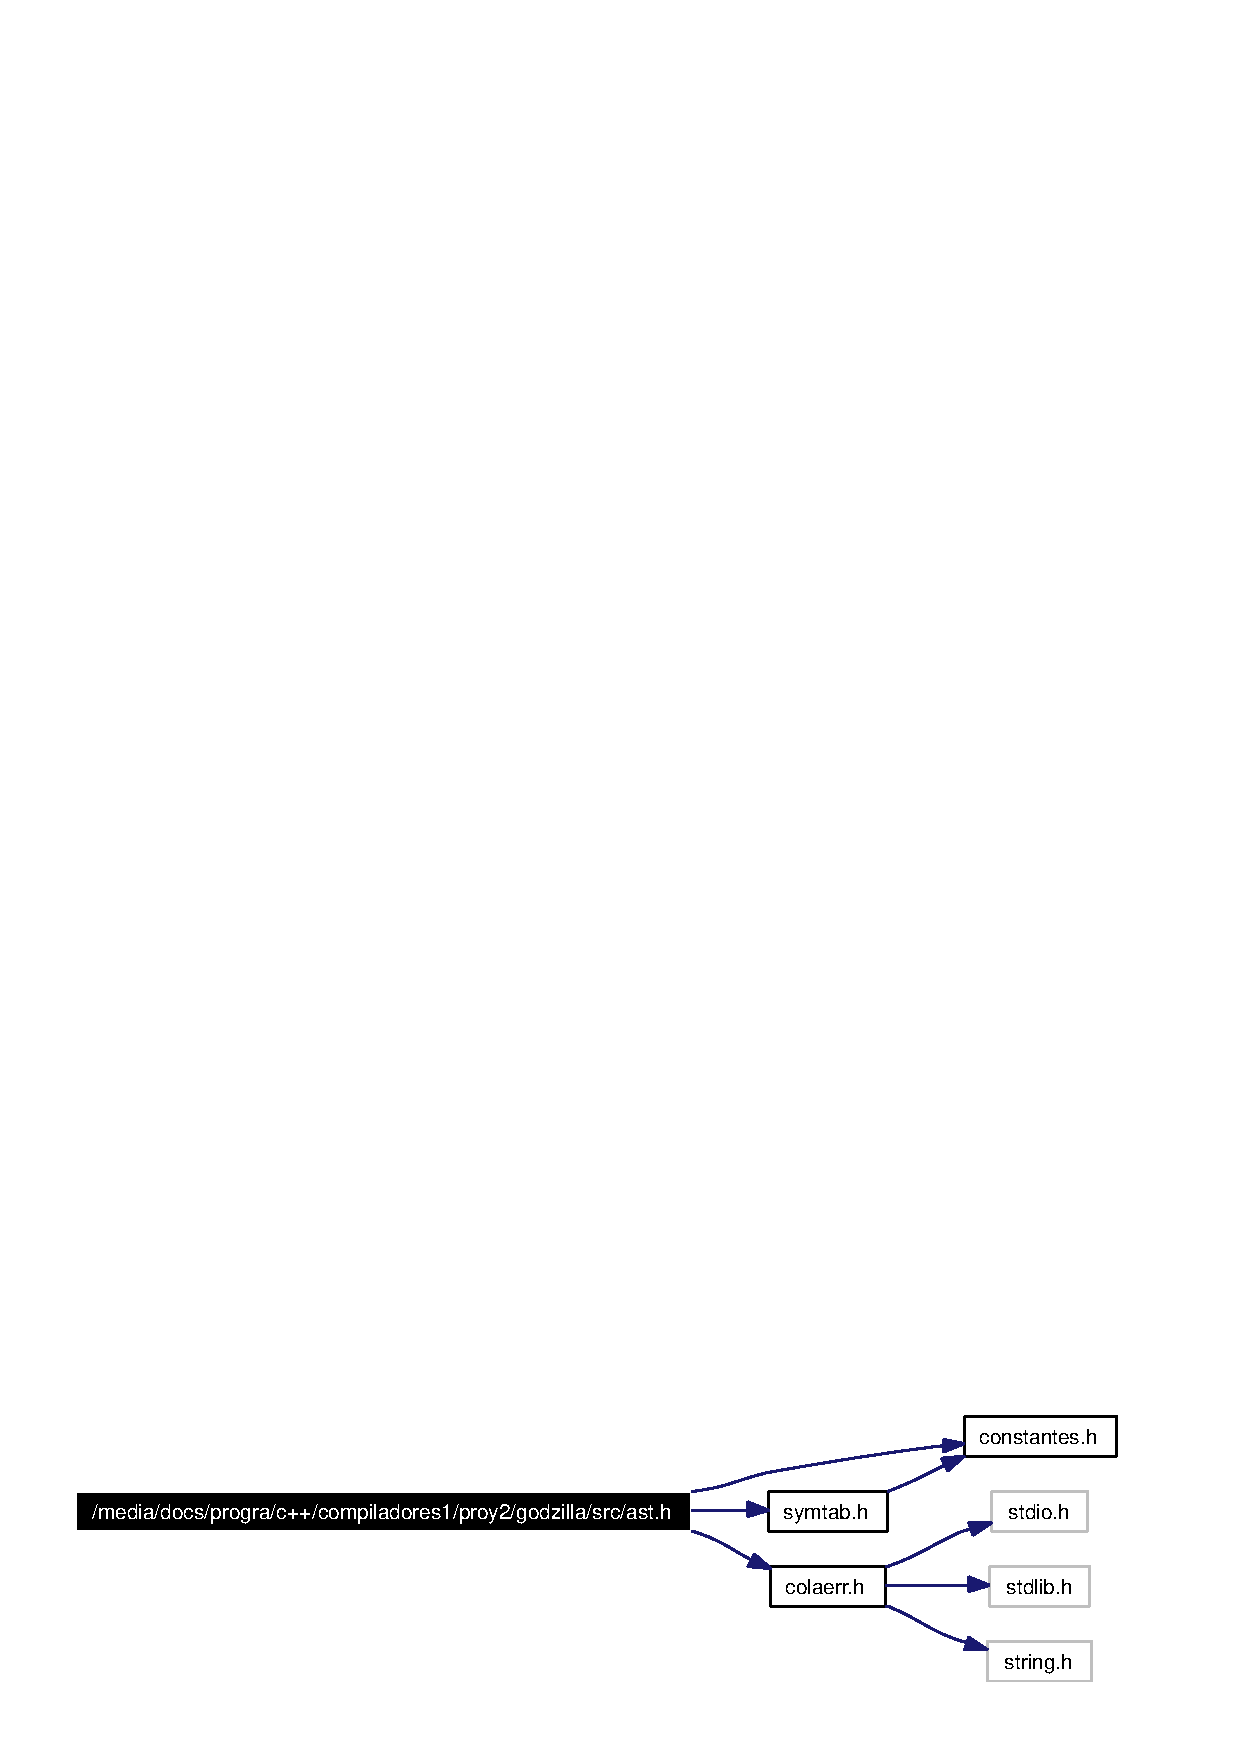
\includegraphics[width=268pt]{ast_8h__incl}
\end{center}
\end{figure}


Este gr\'{a}fico muestra que archivos directa o indirectamente incluyen a este archivo:\begin{figure}[H]
\begin{center}
\leavevmode
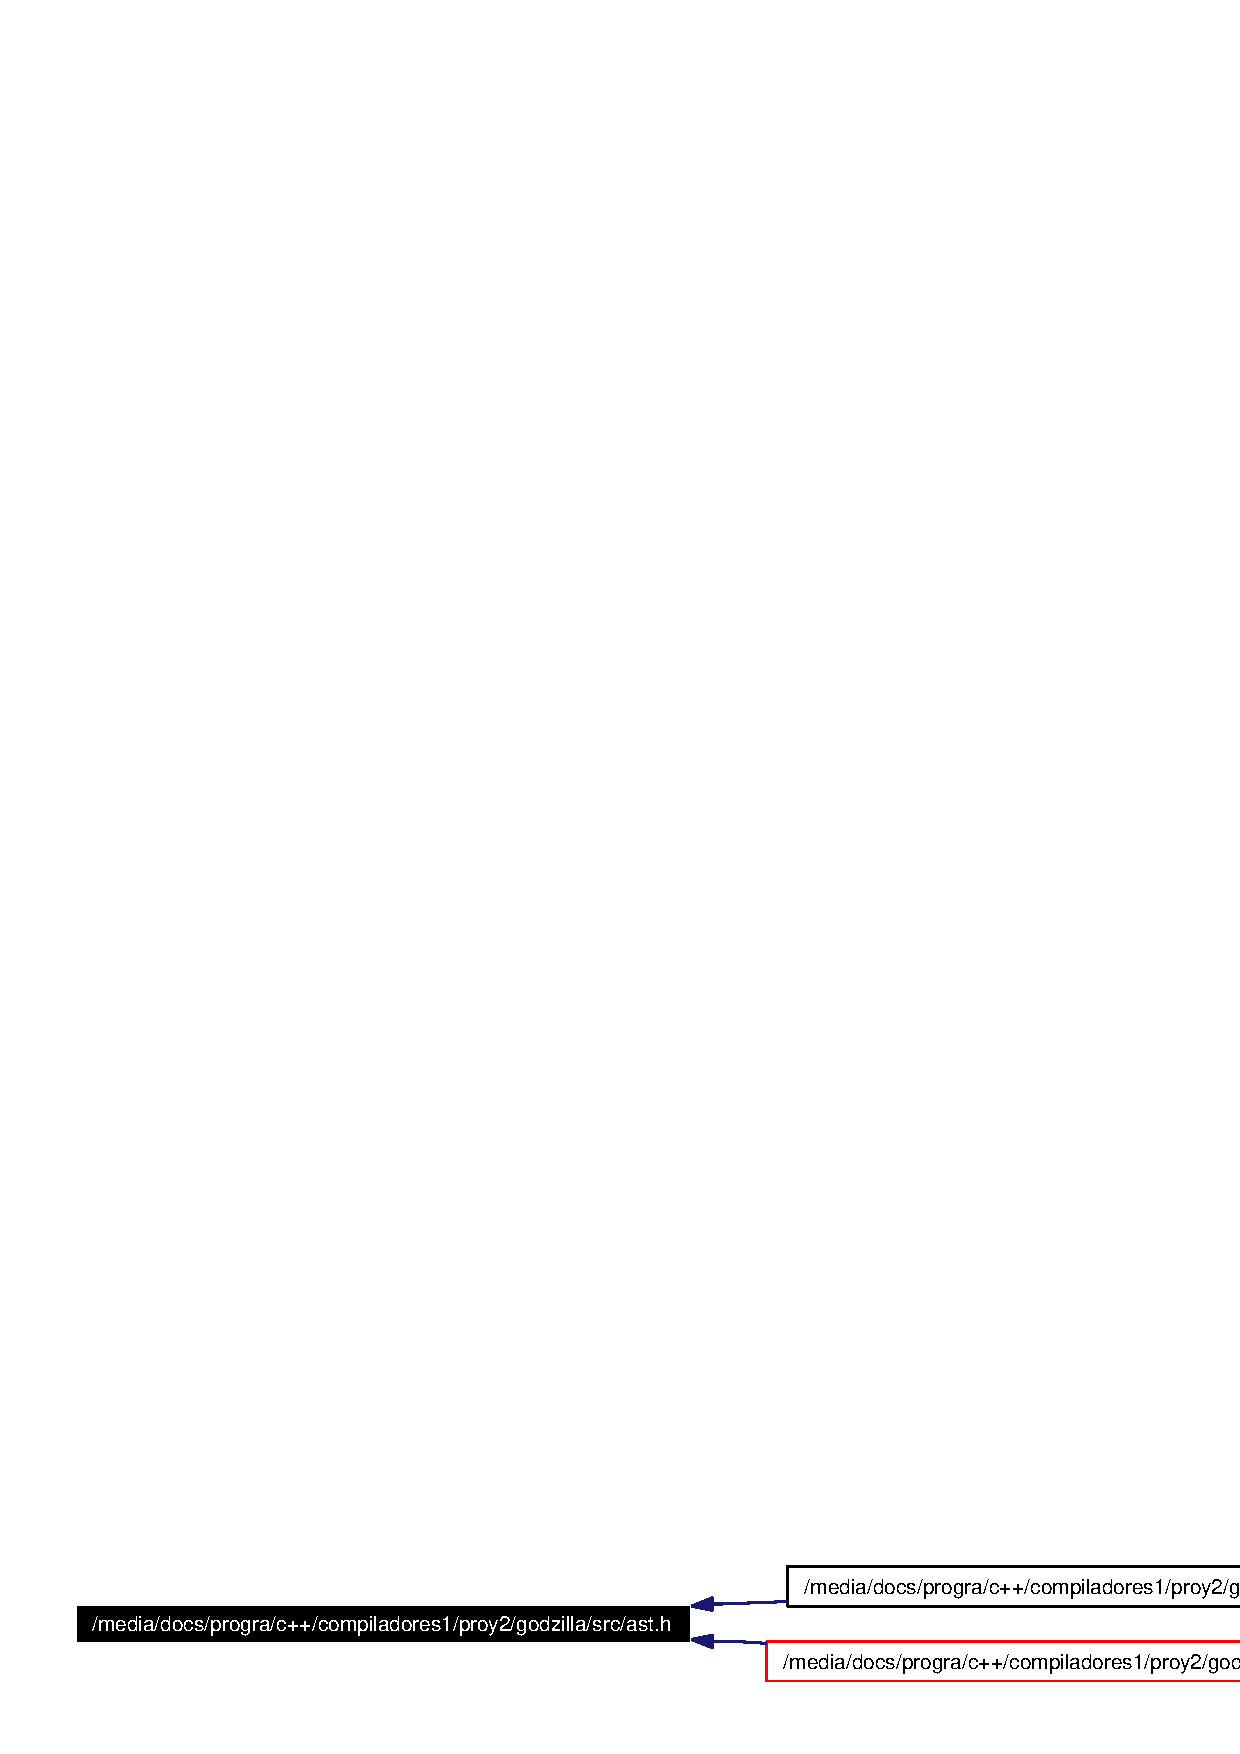
\includegraphics[width=342pt]{ast_8h__dep__incl}
\end{center}
\end{figure}
\subsection*{Clases}
\begin{CompactItemize}
\item 
struct {\bf variable}
\begin{CompactList}\small\item\em Clase de almacenamiento de variables en el AST. \item\end{CompactList}\item 
struct {\bf constante}
\begin{CompactList}\small\item\em Clase de almacenamiento de constantes en el AST. \item\end{CompactList}\item 
struct {\bf operacion}
\begin{CompactList}\small\item\em Clase de almacenamiento de operaciones en el AST. \item\end{CompactList}\item 
struct {\bf enunciado\-If}
\begin{CompactList}\small\item\em Clase de almacenamiento de enunciados If en el AST. \item\end{CompactList}\item 
struct {\bf enunciado\-While}
\begin{CompactList}\small\item\em Clase de almacenamiento de enunciados while en el AST. \item\end{CompactList}\item 
struct {\bf enunciado\-For}
\begin{CompactList}\small\item\em Clase de almacenamiento de enunciados for en el AST. \item\end{CompactList}\item 
struct {\bf expr}
\begin{CompactList}\small\item\em Clase de almacenamiento de raiz de un arbol de expresiones en el AST. \item\end{CompactList}\item 
struct {\bf asignacion}
\begin{CompactList}\small\item\em Clase de almacenamiento de una asignacion en el AST. \item\end{CompactList}\item 
struct {\bf print\-Call}
\begin{CompactList}\small\item\em Clase de almacenamiento de una llamada a Print o a vartablasimbolos en el AST. \item\end{CompactList}\item 
struct {\bf sentencia}
\begin{CompactList}\small\item\em Clase de almacenamiento de raiz de un arbol de sentencias en el AST, siendo a su vez una lista. \item\end{CompactList}\item 
struct {\bf token}
\begin{CompactList}\small\item\em Clase de almacenamiento de raiz de una lista enlazada de Tokens a imprimir con el comando Print en el AST. \item\end{CompactList}\item 
struct {\bf declaracion}
\begin{CompactList}\small\item\em Clase de almacenamiento de raiz de una declaracion en el AST. \item\end{CompactList}\item 
struct {\bf nodo\-Hijo}
\begin{CompactList}\small\item\em Nodo a usar para pasar entre producciones de la sintaxis, y paso de expresiones al recorrer un arbol de expresiones. \item\end{CompactList}\item 
struct {\bf raiz}
\begin{CompactList}\small\item\em punto de entrada del AST \item\end{CompactList}\item 
struct {\bf ast}
\begin{CompactList}\small\item\em Estructura del arbol abstracto de sintaxis (AST), basico para poder evaluar construcciones iterativas del lenguaje. \item\end{CompactList}\end{CompactItemize}
\subsection*{Definiciones}
\begin{CompactItemize}
\item 
\#define {\bf yyout}~embedout
\begin{CompactList}\small\item\em Aliases de yacc en QT, cambiar a nombre de parser a utilizar. \item\end{CompactList}\end{CompactItemize}
\subsection*{Tipos definidos}
\begin{CompactItemize}
\item 
typedef {\bf sentencia} {\bf sentencia}
\item 
typedef {\bf variable} {\bf variable}
\item 
typedef {\bf constante} {\bf constante}
\item 
typedef {\bf operacion} {\bf operacion}
\item 
typedef {\bf enunciado\-If} {\bf enunciado\-If}
\item 
typedef {\bf enunciado\-While} {\bf enunciado\-While}
\item 
typedef {\bf enunciado\-For} {\bf enunciado\-For}
\item 
typedef {\bf expr} {\bf expr}
\item 
typedef {\bf asignacion} {\bf asignacion}
\item 
typedef {\bf print\-Call} {\bf print\-Call}
\item 
typedef {\bf token} {\bf token}
\item 
typedef {\bf declaracion} {\bf declaracion}
\item 
typedef {\bf enunciado} {\bf enunciado}
\item 
typedef {\bf nodo\-Hijo} {\bf nodo}
\item 
typedef {\bf raiz} {\bf raiz}
\item 
typedef {\bf ast} {\bf ast}
\end{CompactItemize}
\subsection*{Funciones}
\begin{CompactItemize}
\item 
{\bf nodo} $\ast$ {\bf insertar\-Constante} (int, int)
\begin{CompactList}\small\item\em Agrega una constante al arbol de expresiones. \item\end{CompactList}\item 
{\bf nodo} $\ast$ {\bf insertar\-Variable} (char $\ast$)
\begin{CompactList}\small\item\em Agrega una variable al arbol de expresiones. \item\end{CompactList}\item 
{\bf nodo} $\ast$ {\bf insertar\-Cadena} (char $\ast$)
\begin{CompactList}\small\item\em Agrega una cadena al arbol de expresiones. \item\end{CompactList}\item 
{\bf nodo} $\ast$ {\bf insertar\-Operacion} (int, {\bf nodo} $\ast$, {\bf nodo} $\ast$)
\begin{CompactList}\small\item\em Inserta una operacion al arbol de expresiones. \item\end{CompactList}\item 
{\bf nodo} $\ast$ {\bf insertar\-Expresion} ({\bf nodo} $\ast$)
\begin{CompactList}\small\item\em Agrega un nuevo arbol de expresiones al arbol principal. \item\end{CompactList}\item 
{\bf nodo} $\ast$ {\bf insertar\-Asignacion} (char $\ast$, {\bf nodo} $\ast$)
\begin{CompactList}\small\item\em Agrega una asignacion al arbol principal. \item\end{CompactList}\item 
{\bf nodo} $\ast$ {\bf insertar\-Sentencia} (int, {\bf nodo} $\ast$, int)
\begin{CompactList}\small\item\em agrega una sentencia al arbol principal \item\end{CompactList}\item 
{\bf nodo} $\ast$ {\bf insertar\-Declaracion} (char $\ast$, int)
\begin{CompactList}\small\item\em agrega una nuva declaracion al arbol principal \item\end{CompactList}\item 
{\bf nodo} $\ast$ {\bf insertar\-Enunciado\-If} ({\bf nodo} $\ast$, {\bf nodo} $\ast$, {\bf nodo} $\ast$)
\begin{CompactList}\small\item\em Agrega un nuevo enunciado if al arbol de sentencias. \item\end{CompactList}\item 
{\bf nodo} $\ast$ {\bf insertar\-Ciclo\-While} ({\bf nodo} $\ast$, {\bf nodo} $\ast$)
\begin{CompactList}\small\item\em Agrega un nuevo ciclo while ar arbol de sentecias. \item\end{CompactList}\item 
{\bf nodo} $\ast$ {\bf insertar\-Ciclo\-For} (char $\ast$, int, int, {\bf nodo} $\ast$)
\begin{CompactList}\small\item\em Agrega un nuevo ciclo for al arbol de sentencias. \item\end{CompactList}\item 
{\bf nodo} $\ast$ {\bf insertar\-Token} (int, void $\ast$)
\begin{CompactList}\small\item\em Agrega un nuevo token al arbol de sentencias. \item\end{CompactList}\item 
{\bf nodo} $\ast$ {\bf insertar\-Llamada} ({\bf nodo} $\ast$)
\begin{CompactList}\small\item\em Agrega un nueva llamada de impresion a yyout al arbol de sentencias. \item\end{CompactList}\item 
{\bf nodo} $\ast$ {\bf insertar\-Llamada\-Sym\-Tab} (int)
\begin{CompactList}\small\item\em Agrega un nueva llamada de impresion de tabla de simbolos al arbol de sentencias. \item\end{CompactList}\item 
{\bf nodo} $\ast$ {\bf concatenar\-Tokens} ({\bf nodo} $\ast$, {\bf nodo} $\ast$)
\begin{CompactList}\small\item\em Concatena tokens para parametros de llamadas. \item\end{CompactList}\item 
{\bf nodo} $\ast$ {\bf concatenar\-Sentencia} ({\bf nodo} $\ast$, {\bf nodo} $\ast$)
\begin{CompactList}\small\item\em Concatena sentencias para caminar por estas. \item\end{CompactList}\item 
void {\bf crear\-Raiz} ({\bf nodo} $\ast$, {\bf ast} $\ast$)
\begin{CompactList}\small\item\em Genera el nodo raiz para el arbol dado en el segundo parametro como punto de inicio del arbol y punto de meta del recorrido sintactico. \item\end{CompactList}\item 
{\bf nodo} $\ast$ {\bf ref\-Nodo\-Hijo} (int tipo, void $\ast$dato)
\begin{CompactList}\small\item\em Crea un nodo que refiere al nodo recien creado para sea utilizado por el nodo anterior a este. \item\end{CompactList}\item 
int {\bf recorrer\-Arbol} ({\bf ast} $\ast$tree, char $\ast$filename)
\begin{CompactList}\small\item\em Recorre el arbol y escribe resultado en archivo salida. \item\end{CompactList}\item 
int {\bf recorrer\-Sentencia} ({\bf sentencia} $\ast$s)
\begin{CompactList}\small\item\em Recorre sentencias recursivamente y devuelve resultado acarreado. \item\end{CompactList}\item 
int {\bf evaluar\-Sentencia} ({\bf sentencia} $\ast$s)
\begin{CompactList}\small\item\em Evalua sentencia y selecciona tipo de sentencia a evaluar. \item\end{CompactList}\item 
int {\bf evaluar\-Declaracion} ({\bf declaracion} $\ast$d)
\begin{CompactList}\small\item\em Evalua declaracion. \item\end{CompactList}\item 
int {\bf evaluar\-Asignacion} ({\bf asignacion} $\ast$a)
\begin{CompactList}\small\item\em Evalua asignacion. \item\end{CompactList}\item 
{\bf nodo} $\ast$ {\bf evaluar\-Expresion} ({\bf expr} $\ast$e)
\begin{CompactList}\small\item\em Evalua expresion y selecciona tipo de expresion a evaluar. \item\end{CompactList}\item 
{\bf nodo} $\ast$ {\bf evaluar\-Operacion} ({\bf operacion} $\ast$o)
\begin{CompactList}\small\item\em Selecciona operacion binaria a evaluar. \item\end{CompactList}\item 
{\bf nodo} $\ast$ {\bf evaluar\-Or} ({\bf nodo} $\ast$n1, {\bf nodo} $\ast$n2)
\begin{CompactList}\small\item\em Evalua operacion logica OR. \item\end{CompactList}\item 
{\bf nodo} $\ast$ {\bf evaluar\-And} ({\bf nodo} $\ast$n1, {\bf nodo} $\ast$n2)
\begin{CompactList}\small\item\em Evalua operacion logica AND. \item\end{CompactList}\item 
{\bf nodo} $\ast$ {\bf evaluar\-GT} ({\bf nodo} $\ast$n1, {\bf nodo} $\ast$n2)
\begin{CompactList}\small\item\em Evalua operacion comparativa Mayor Que. \item\end{CompactList}\item 
{\bf nodo} $\ast$ {\bf evaluar\-GET} ({\bf nodo} $\ast$n1, {\bf nodo} $\ast$n2)
\begin{CompactList}\small\item\em Evalua operacion comparativa Mayor o igual Que. \item\end{CompactList}\item 
{\bf nodo} $\ast$ {\bf evaluar\-LT} ({\bf nodo} $\ast$n1, {\bf nodo} $\ast$n2)
\begin{CompactList}\small\item\em Evalua operacion comparativa Menor Que. \item\end{CompactList}\item 
{\bf nodo} $\ast$ {\bf evaluar\-LET} ({\bf nodo} $\ast$n1, {\bf nodo} $\ast$n2)
\begin{CompactList}\small\item\em Evalua operacion comparativa Menor o Igual Que. \item\end{CompactList}\item 
{\bf nodo} $\ast$ {\bf evaluar\-EQ} ({\bf nodo} $\ast$n1, {\bf nodo} $\ast$n2)
\begin{CompactList}\small\item\em Evalua operacion comparativa Igual. \item\end{CompactList}\item 
{\bf nodo} $\ast$ {\bf evaluar\-NEQ} ({\bf nodo} $\ast$n1, {\bf nodo} $\ast$n2)
\begin{CompactList}\small\item\em Evalua operacion comparativa Desigual. \item\end{CompactList}\item 
{\bf nodo} $\ast$ {\bf evaluar\-Suma} ({\bf nodo} $\ast$n1, {\bf nodo} $\ast$n2)
\begin{CompactList}\small\item\em Evalua operacion aritmetica Suma, y la concatenacion de cadenas. \item\end{CompactList}\item 
{\bf nodo} $\ast$ {\bf evaluar\-Resta} ({\bf nodo} $\ast$n1, {\bf nodo} $\ast$n2)
\begin{CompactList}\small\item\em Evalua operacion aritmetica Resta. \item\end{CompactList}\item 
{\bf nodo} $\ast$ {\bf evaluar\-Mult} ({\bf nodo} $\ast$n1, {\bf nodo} $\ast$n2)
\begin{CompactList}\small\item\em Evalua operacion aritmetica Multiplicacion. \item\end{CompactList}\item 
{\bf nodo} $\ast$ {\bf evaluar\-Div} ({\bf nodo} $\ast$n1, {\bf nodo} $\ast$n2)
\begin{CompactList}\small\item\em Evalua operacion aritmetica Division. \item\end{CompactList}\item 
int {\bf evaluar\-If} ({\bf enunciado\-If} $\ast$eif)
\begin{CompactList}\small\item\em Evalua bifurcacion If. \item\end{CompactList}\item 
int {\bf evaluar\-While} ({\bf enunciado\-While} $\ast$ew)
\begin{CompactList}\small\item\em Evalua bucle While. \item\end{CompactList}\item 
int {\bf evaluar\-For} ({\bf enunciado\-For} $\ast$ef)
\begin{CompactList}\small\item\em Evalua bucle For. \item\end{CompactList}\item 
int {\bf evaluar\-Print\-Call} ({\bf print\-Call} $\ast$pc)
\begin{CompactList}\small\item\em Evalua llamada a imprimir en archivo. \item\end{CompactList}\item 
int {\bf imprimir\-Tokens} ({\bf token} $\ast$t)
\begin{CompactList}\small\item\em Evalua recursivamente lista de tokens a imprimir. \item\end{CompactList}\item 
void {\bf error} (char $\ast$err, int tipo, void $\ast$dato)
\begin{CompactList}\small\item\em Escribe error semantico hacia cola de errores semanticos. \item\end{CompactList}\item 
void {\bf borrar\-Arbol} ({\bf ast} $\ast$tree)
\begin{CompactList}\small\item\em Funciones de eliminacion logica. \item\end{CompactList}\item 
void {\bf borrar\-Sentencias} ({\bf sentencia} $\ast$s)
\begin{CompactList}\small\item\em Borra nodo sentencia. \item\end{CompactList}\item 
void {\bf borrar\-Declaracion} ({\bf declaracion} $\ast$d)
\begin{CompactList}\small\item\em Borra nodo declaracion. \item\end{CompactList}\item 
void {\bf borrar\-Asignacion} ({\bf asignacion} $\ast$a)
\begin{CompactList}\small\item\em Borrar Asignacion. \item\end{CompactList}\item 
void {\bf borrar\-Expresion} ({\bf expr} $\ast$e)
\begin{CompactList}\small\item\em Elimina de memoria arbol de expresiones. \item\end{CompactList}\item 
void {\bf borrar\-Operacion} ({\bf operacion} $\ast$o)
\begin{CompactList}\small\item\em borra nodo operacion de mem \item\end{CompactList}\item 
void {\bf borrar\-If} ({\bf enunciado\-If} $\ast$eif)
\begin{CompactList}\small\item\em borra nodo if \item\end{CompactList}\item 
void {\bf borrar\-While} ({\bf enunciado\-While} $\ast$ew)
\begin{CompactList}\small\item\em borra nodo While \item\end{CompactList}\item 
void {\bf borrar\-For} ({\bf enunciado\-For} $\ast$ef)
\begin{CompactList}\small\item\em borra nodo for \item\end{CompactList}\item 
void {\bf borrar\-Print\-Call} ({\bf print\-Call} $\ast$pc)
\begin{CompactList}\small\item\em borra nodo de llamada a imprimir en archivo \item\end{CompactList}\item 
void {\bf borrar\-Tokens} ({\bf token} $\ast$t)
\begin{CompactList}\small\item\em borra recursivamente listado de tokens \item\end{CompactList}\end{CompactItemize}


\subsection{Descripci\'{o}n detallada}
Definiciones y estructura del arbol de sintaxis abstracta. 



Definici\'{o}n en el archivo {\bf ast.h}.

\subsection{Documentaci\'{o}n de las definiciones}
\index{ast.h@{ast.h}!yyout@{yyout}}
\index{yyout@{yyout}!ast.h@{ast.h}}
\subsubsection{\setlength{\rightskip}{0pt plus 5cm}\#define {\bf yyout}~embedout}\label{ast_8h_a0}


Aliases de yacc en QT, cambiar a nombre de parser a utilizar. 



Definici\'{o}n en la l\'{\i}nea 11 del archivo ast.h.

Referenciado por imprimir\-Tokens().

\subsection{Documentaci\'{o}n de los tipos definidos}
\index{ast.h@{ast.h}!asignacion@{asignacion}}
\index{asignacion@{asignacion}!ast.h@{ast.h}}
\subsubsection{\setlength{\rightskip}{0pt plus 5cm}typedef struct {\bf asignacion} {\bf asignacion}}\label{ast_8h_a9}




Definici\'{o}n en la l\'{\i}nea 31 del archivo ast.h.\index{ast.h@{ast.h}!ast@{ast}}
\index{ast@{ast}!ast.h@{ast.h}}
\subsubsection{\setlength{\rightskip}{0pt plus 5cm}typedef struct {\bf ast} {\bf ast}}\label{ast_8h_a16}




Definici\'{o}n en la l\'{\i}nea 38 del archivo ast.h.\index{ast.h@{ast.h}!constante@{constante}}
\index{constante@{constante}!ast.h@{ast.h}}
\subsubsection{\setlength{\rightskip}{0pt plus 5cm}typedef struct {\bf constante} {\bf constante}}\label{ast_8h_a3}




Definici\'{o}n en la l\'{\i}nea 25 del archivo ast.h.\index{ast.h@{ast.h}!declaracion@{declaracion}}
\index{declaracion@{declaracion}!ast.h@{ast.h}}
\subsubsection{\setlength{\rightskip}{0pt plus 5cm}typedef struct {\bf declaracion} {\bf declaracion}}\label{ast_8h_a12}




Definici\'{o}n en la l\'{\i}nea 34 del archivo ast.h.\index{ast.h@{ast.h}!enunciado@{enunciado}}
\index{enunciado@{enunciado}!ast.h@{ast.h}}
\subsubsection{\setlength{\rightskip}{0pt plus 5cm}typedef struct {\bf enunciado} {\bf enunciado}}\label{ast_8h_a13}




Definici\'{o}n en la l\'{\i}nea 35 del archivo ast.h.\index{ast.h@{ast.h}!enunciadoFor@{enunciadoFor}}
\index{enunciadoFor@{enunciadoFor}!ast.h@{ast.h}}
\subsubsection{\setlength{\rightskip}{0pt plus 5cm}typedef struct {\bf enunciado\-For} {\bf enunciado\-For}}\label{ast_8h_a7}




Definici\'{o}n en la l\'{\i}nea 29 del archivo ast.h.\index{ast.h@{ast.h}!enunciadoIf@{enunciadoIf}}
\index{enunciadoIf@{enunciadoIf}!ast.h@{ast.h}}
\subsubsection{\setlength{\rightskip}{0pt plus 5cm}typedef struct {\bf enunciado\-If} {\bf enunciado\-If}}\label{ast_8h_a5}




Definici\'{o}n en la l\'{\i}nea 27 del archivo ast.h.\index{ast.h@{ast.h}!enunciadoWhile@{enunciadoWhile}}
\index{enunciadoWhile@{enunciadoWhile}!ast.h@{ast.h}}
\subsubsection{\setlength{\rightskip}{0pt plus 5cm}typedef struct {\bf enunciado\-While} {\bf enunciado\-While}}\label{ast_8h_a6}




Definici\'{o}n en la l\'{\i}nea 28 del archivo ast.h.\index{ast.h@{ast.h}!expr@{expr}}
\index{expr@{expr}!ast.h@{ast.h}}
\subsubsection{\setlength{\rightskip}{0pt plus 5cm}typedef struct {\bf expr} {\bf expr}}\label{ast_8h_a8}




Definici\'{o}n en la l\'{\i}nea 30 del archivo ast.h.\index{ast.h@{ast.h}!nodo@{nodo}}
\index{nodo@{nodo}!ast.h@{ast.h}}
\subsubsection{\setlength{\rightskip}{0pt plus 5cm}typedef struct {\bf nodo\-Hijo} {\bf nodo}}\label{ast_8h_a14}




Definici\'{o}n en la l\'{\i}nea 36 del archivo ast.h.\index{ast.h@{ast.h}!operacion@{operacion}}
\index{operacion@{operacion}!ast.h@{ast.h}}
\subsubsection{\setlength{\rightskip}{0pt plus 5cm}typedef struct {\bf operacion} {\bf operacion}}\label{ast_8h_a4}




Definici\'{o}n en la l\'{\i}nea 26 del archivo ast.h.\index{ast.h@{ast.h}!printCall@{printCall}}
\index{printCall@{printCall}!ast.h@{ast.h}}
\subsubsection{\setlength{\rightskip}{0pt plus 5cm}typedef struct {\bf print\-Call} {\bf print\-Call}}\label{ast_8h_a10}




Definici\'{o}n en la l\'{\i}nea 32 del archivo ast.h.\index{ast.h@{ast.h}!raiz@{raiz}}
\index{raiz@{raiz}!ast.h@{ast.h}}
\subsubsection{\setlength{\rightskip}{0pt plus 5cm}typedef struct {\bf raiz} {\bf raiz}}\label{ast_8h_a15}




Definici\'{o}n en la l\'{\i}nea 37 del archivo ast.h.\index{ast.h@{ast.h}!sentencia@{sentencia}}
\index{sentencia@{sentencia}!ast.h@{ast.h}}
\subsubsection{\setlength{\rightskip}{0pt plus 5cm}typedef struct {\bf sentencia} {\bf sentencia}}\label{ast_8h_a1}




Definici\'{o}n en la l\'{\i}nea 23 del archivo ast.h.\index{ast.h@{ast.h}!token@{token}}
\index{token@{token}!ast.h@{ast.h}}
\subsubsection{\setlength{\rightskip}{0pt plus 5cm}typedef struct {\bf token} {\bf token}}\label{ast_8h_a11}




Definici\'{o}n en la l\'{\i}nea 33 del archivo ast.h.\index{ast.h@{ast.h}!variable@{variable}}
\index{variable@{variable}!ast.h@{ast.h}}
\subsubsection{\setlength{\rightskip}{0pt plus 5cm}typedef struct {\bf variable} {\bf variable}}\label{ast_8h_a2}




Definici\'{o}n en la l\'{\i}nea 24 del archivo ast.h.

\subsection{Documentaci\'{o}n de las funciones}
\index{ast.h@{ast.h}!borrarArbol@{borrarArbol}}
\index{borrarArbol@{borrarArbol}!ast.h@{ast.h}}
\subsubsection{\setlength{\rightskip}{0pt plus 5cm}void borrar\-Arbol ({\bf ast} $\ast$ {\em tree})}\label{ast_8h_a60}


Funciones de eliminacion logica. 



Definici\'{o}n en la l\'{\i}nea 897 del archivo ast.c.

Hace referencia a ast::actual, borrar\-Sentencias(), raiz::hijo, ast::root, y ast::tipo\-Actual.\index{ast.h@{ast.h}!borrarAsignacion@{borrarAsignacion}}
\index{borrarAsignacion@{borrarAsignacion}!ast.h@{ast.h}}
\subsubsection{\setlength{\rightskip}{0pt plus 5cm}void borrar\-Asignacion ({\bf asignacion} $\ast$ {\em a})}\label{ast_8h_a63}


Borrar Asignacion. 



Definici\'{o}n en la l\'{\i}nea 952 del archivo ast.c.

Hace referencia a borrar\-Expresion(), asignacion::hijo, y asignacion::variable.

Referenciado por borrar\-Sentencias().\index{ast.h@{ast.h}!borrarDeclaracion@{borrarDeclaracion}}
\index{borrarDeclaracion@{borrarDeclaracion}!ast.h@{ast.h}}
\subsubsection{\setlength{\rightskip}{0pt plus 5cm}void borrar\-Declaracion ({\bf declaracion} $\ast$ {\em d})}\label{ast_8h_a62}


Borra nodo declaracion. 



Definici\'{o}n en la l\'{\i}nea 943 del archivo ast.c.

Hace referencia a declaracion::identificador.

Referenciado por borrar\-Sentencias().\index{ast.h@{ast.h}!borrarExpresion@{borrarExpresion}}
\index{borrarExpresion@{borrarExpresion}!ast.h@{ast.h}}
\subsubsection{\setlength{\rightskip}{0pt plus 5cm}void borrar\-Expresion ({\bf expr} $\ast$ {\em e})}\label{ast_8h_a64}


Elimina de memoria arbol de expresiones. 



Definici\'{o}n en la l\'{\i}nea 962 del archivo ast.c.

Hace referencia a borrar\-Operacion(), expr::hijo, T\_\-CONSTANTE, T\_\-LITERAL, T\_\-OPERACION, T\_\-VARIABLE, y expr::tipo.

Referenciado por borrar\-Asignacion(), borrar\-If(), borrar\-Operacion(), y borrar\-While().\index{ast.h@{ast.h}!borrarFor@{borrarFor}}
\index{borrarFor@{borrarFor}!ast.h@{ast.h}}
\subsubsection{\setlength{\rightskip}{0pt plus 5cm}void borrar\-For ({\bf enunciado\-For} $\ast$ {\em ef})}\label{ast_8h_a68}


borra nodo for 



Definici\'{o}n en la l\'{\i}nea 1017 del archivo ast.c.

Hace referencia a borrar\-Sentencias(), enunciado\-For::cuerpo, y enunciado\-For::indice.

Referenciado por borrar\-Sentencias().\index{ast.h@{ast.h}!borrarIf@{borrarIf}}
\index{borrarIf@{borrarIf}!ast.h@{ast.h}}
\subsubsection{\setlength{\rightskip}{0pt plus 5cm}void borrar\-If ({\bf enunciado\-If} $\ast$ {\em eif})}\label{ast_8h_a66}


borra nodo if 



Definici\'{o}n en la l\'{\i}nea 995 del archivo ast.c.

Hace referencia a borrar\-Expresion(), borrar\-Sentencias(), enunciado\-If::else\_\-stmt, enunciado\-If::test, y enunciado\-If::then\_\-stmt.

Referenciado por borrar\-Sentencias().\index{ast.h@{ast.h}!borrarOperacion@{borrarOperacion}}
\index{borrarOperacion@{borrarOperacion}!ast.h@{ast.h}}
\subsubsection{\setlength{\rightskip}{0pt plus 5cm}void borrar\-Operacion ({\bf operacion} $\ast$ {\em o})}\label{ast_8h_a65}


borra nodo operacion de mem 



Definici\'{o}n en la l\'{\i}nea 985 del archivo ast.c.

Hace referencia a borrar\-Expresion(), operacion::loper, y operacion::roper.

Referenciado por borrar\-Expresion().\index{ast.h@{ast.h}!borrarPrintCall@{borrarPrintCall}}
\index{borrarPrintCall@{borrarPrintCall}!ast.h@{ast.h}}
\subsubsection{\setlength{\rightskip}{0pt plus 5cm}void borrar\-Print\-Call ({\bf print\-Call} $\ast$ {\em pc})}\label{ast_8h_a69}


borra nodo de llamada a imprimir en archivo 



Definici\'{o}n en la l\'{\i}nea 1026 del archivo ast.c.

Hace referencia a borrar\-Tokens(), y print\-Call::hijos.

Referenciado por borrar\-Sentencias().\index{ast.h@{ast.h}!borrarSentencias@{borrarSentencias}}
\index{borrarSentencias@{borrarSentencias}!ast.h@{ast.h}}
\subsubsection{\setlength{\rightskip}{0pt plus 5cm}void borrar\-Sentencias ({\bf sentencia} $\ast$ {\em s})}\label{ast_8h_a61}


Borra nodo sentencia. 



Definici\'{o}n en la l\'{\i}nea 914 del archivo ast.c.

Hace referencia a borrar\-Asignacion(), borrar\-Declaracion(), borrar\-For(), borrar\-If(), borrar\-Print\-Call(), borrar\-Sentencias(), borrar\-While(), sentencia::hijo, sentencia::siguiente, T\_\-ASIGNACION, T\_\-CALL, T\_\-DECLARACION, T\_\-FOR, T\_\-IF, T\_\-WHILE, y sentencia::tipo.

Referenciado por borrar\-Arbol(), borrar\-For(), borrar\-If(), borrar\-Sentencias(), y borrar\-While().\index{ast.h@{ast.h}!borrarTokens@{borrarTokens}}
\index{borrarTokens@{borrarTokens}!ast.h@{ast.h}}
\subsubsection{\setlength{\rightskip}{0pt plus 5cm}void borrar\-Tokens ({\bf token} $\ast$ {\em t})}\label{ast_8h_a70}


borra recursivamente listado de tokens 



Definici\'{o}n en la l\'{\i}nea 1036 del archivo ast.c.

Hace referencia a borrar\-Tokens(), token::hijo, token::siguiente, T\_\-CADENA, T\_\-STRING, y token::tipo.

Referenciado por borrar\-Print\-Call(), y borrar\-Tokens().\index{ast.h@{ast.h}!borrarWhile@{borrarWhile}}
\index{borrarWhile@{borrarWhile}!ast.h@{ast.h}}
\subsubsection{\setlength{\rightskip}{0pt plus 5cm}void borrar\-While ({\bf enunciado\-While} $\ast$ {\em ew})}\label{ast_8h_a67}


borra nodo While 



Definici\'{o}n en la l\'{\i}nea 1008 del archivo ast.c.

Hace referencia a borrar\-Expresion(), borrar\-Sentencias(), enunciado\-While::cuerpo, y enunciado\-While::test.

Referenciado por borrar\-Sentencias().\index{ast.h@{ast.h}!concatenarSentencia@{concatenarSentencia}}
\index{concatenarSentencia@{concatenarSentencia}!ast.h@{ast.h}}
\subsubsection{\setlength{\rightskip}{0pt plus 5cm}{\bf nodo}$\ast$ concatenar\-Sentencia ({\bf nodo} $\ast$, {\bf nodo} $\ast$)}\label{ast_8h_a32}


Concatena sentencias para caminar por estas. 



Definici\'{o}n en la l\'{\i}nea 140 del archivo ast.c.

Hace referencia a nodo\-Hijo::dato, y sentencia::siguiente.\index{ast.h@{ast.h}!concatenarTokens@{concatenarTokens}}
\index{concatenarTokens@{concatenarTokens}!ast.h@{ast.h}}
\subsubsection{\setlength{\rightskip}{0pt plus 5cm}{\bf nodo}$\ast$ concatenar\-Tokens ({\bf nodo} $\ast$, {\bf nodo} $\ast$)}\label{ast_8h_a31}


Concatena tokens para parametros de llamadas. 



Definici\'{o}n en la l\'{\i}nea 231 del archivo ast.c.

Hace referencia a nodo\-Hijo::dato, y token::siguiente.\index{ast.h@{ast.h}!crearRaiz@{crearRaiz}}
\index{crearRaiz@{crearRaiz}!ast.h@{ast.h}}
\subsubsection{\setlength{\rightskip}{0pt plus 5cm}void crear\-Raiz ({\bf nodo} $\ast$, {\bf ast} $\ast$)}\label{ast_8h_a33}


Genera el nodo raiz para el arbol dado en el segundo parametro como punto de inicio del arbol y punto de meta del recorrido sintactico. 



Definici\'{o}n en la l\'{\i}nea 263 del archivo ast.c.

Hace referencia a ast::actual, nodo\-Hijo::dato, raiz::hijo, ast::root, T\_\-SENTENCIA, y ast::tipo\-Actual.\index{ast.h@{ast.h}!error@{error}}
\index{error@{error}!ast.h@{ast.h}}
\subsubsection{\setlength{\rightskip}{0pt plus 5cm}void error (char $\ast$ {\em err}, int {\em tipo}, void $\ast$ {\em dato})}\label{ast_8h_a59}


Escribe error semantico hacia cola de errores semanticos. 



Definici\'{o}n en la l\'{\i}nea 280 del archivo ast.c.

Hace referencia a error\-Semantico(), sentencia::num\-Linea, y T\_\-SENTENCIA.

Referenciado por evaluar\-And(), evaluar\-Asignacion(), evaluar\-Declaracion(), evaluar\-Div(), evaluar\-Expresion(), evaluar\-For(), evaluar\-GET(), evaluar\-GT(), evaluar\-If(), evaluar\-LET(), evaluar\-LT(), evaluar\-Mult(), evaluar\-Or(), evaluar\-Print\-Call(), evaluar\-Resta(), evaluar\-Suma(), evaluar\-While(), imprimir\-Tokens(), y recorrer\-Sentencia().\index{ast.h@{ast.h}!evaluarAnd@{evaluarAnd}}
\index{evaluarAnd@{evaluarAnd}!ast.h@{ast.h}}
\subsubsection{\setlength{\rightskip}{0pt plus 5cm}{\bf nodo}$\ast$ evaluar\-And ({\bf nodo} $\ast$ {\em n1}, {\bf nodo} $\ast$ {\em n2})}\label{ast_8h_a43}


Evalua operacion logica AND. 



Definici\'{o}n en la l\'{\i}nea 491 del archivo ast.c.

Hace referencia a nodo\-Hijo::dato, error(), ref\-Nodo\-Hijo(), T\_\-BOOLEAN, T\_\-FALSE, T\_\-OPERACION, T\_\-TRUE, y nodo\-Hijo::tipo.

Referenciado por evaluar\-Operacion().\index{ast.h@{ast.h}!evaluarAsignacion@{evaluarAsignacion}}
\index{evaluarAsignacion@{evaluarAsignacion}!ast.h@{ast.h}}
\subsubsection{\setlength{\rightskip}{0pt plus 5cm}int evaluar\-Asignacion ({\bf asignacion} $\ast$ {\em a})}\label{ast_8h_a39}


Evalua asignacion. 



Definici\'{o}n en la l\'{\i}nea 359 del archivo ast.c.

Hace referencia a buscar\-Simbolo(), nodo\-Hijo::dato, error(), evaluar\-Expresion(), asignacion::hijo, T\_\-ASIGNACION, T\_\-BOOLEAN, T\_\-INTEGER, T\_\-NUMERO, symbol::tipo, nodo\-Hijo::tipo, symbol::valor, y asignacion::variable.

Referenciado por evaluar\-Sentencia().\index{ast.h@{ast.h}!evaluarDeclaracion@{evaluarDeclaracion}}
\index{evaluarDeclaracion@{evaluarDeclaracion}!ast.h@{ast.h}}
\subsubsection{\setlength{\rightskip}{0pt plus 5cm}int evaluar\-Declaracion ({\bf declaracion} $\ast$ {\em d})}\label{ast_8h_a38}


Evalua declaracion. 



Definici\'{o}n en la l\'{\i}nea 350 del archivo ast.c.

Hace referencia a buscar\-Simbolo(), error(), declaracion::identificador, insertar\-Simbolo(), T\_\-DECLARACION, y declaracion::tipo.

Referenciado por evaluar\-Sentencia().\index{ast.h@{ast.h}!evaluarDiv@{evaluarDiv}}
\index{evaluarDiv@{evaluarDiv}!ast.h@{ast.h}}
\subsubsection{\setlength{\rightskip}{0pt plus 5cm}{\bf nodo}$\ast$ evaluar\-Div ({\bf nodo} $\ast$ {\em n1}, {\bf nodo} $\ast$ {\em n2})}\label{ast_8h_a53}


Evalua operacion aritmetica Division. 



Definici\'{o}n en la l\'{\i}nea 671 del archivo ast.c.

Hace referencia a nodo\-Hijo::dato, error(), ref\-Nodo\-Hijo(), T\_\-INTEGER, T\_\-OPERACION, y nodo\-Hijo::tipo.

Referenciado por evaluar\-Operacion().\index{ast.h@{ast.h}!evaluarEQ@{evaluarEQ}}
\index{evaluarEQ@{evaluarEQ}!ast.h@{ast.h}}
\subsubsection{\setlength{\rightskip}{0pt plus 5cm}{\bf nodo}$\ast$ evaluar\-EQ ({\bf nodo} $\ast$ {\em n1}, {\bf nodo} $\ast$ {\em n2})}\label{ast_8h_a48}


Evalua operacion comparativa Igual. 



Definici\'{o}n en la l\'{\i}nea 535 del archivo ast.c.

Hace referencia a nodo\-Hijo::dato, ref\-Nodo\-Hijo(), T\_\-BOOLEAN, T\_\-FALSE, T\_\-INTEGER, T\_\-STRING, T\_\-TRUE, y nodo\-Hijo::tipo.

Referenciado por evaluar\-Operacion().\index{ast.h@{ast.h}!evaluarExpresion@{evaluarExpresion}}
\index{evaluarExpresion@{evaluarExpresion}!ast.h@{ast.h}}
\subsubsection{\setlength{\rightskip}{0pt plus 5cm}{\bf nodo}$\ast$ evaluar\-Expresion ({\bf expr} $\ast$ {\em e})}\label{ast_8h_a40}


Evalua expresion y selecciona tipo de expresion a evaluar. 



Definici\'{o}n en la l\'{\i}nea 391 del archivo ast.c.

Hace referencia a buscar\-Simbolo(), nodo\-Hijo::dato, error(), evaluar\-Operacion(), expr::hijo, T\_\-BOOLEAN, T\_\-CONSTANTE, T\_\-EXPR, T\_\-INTEGER, T\_\-LITERAL, T\_\-NUMERO, T\_\-OPERACION, T\_\-STRING, T\_\-VARIABLE, symbol::tipo, nodo\-Hijo::tipo, expr::tipo, y symbol::valor.

Referenciado por evaluar\-Asignacion(), evaluar\-If(), evaluar\-Operacion(), y evaluar\-While().\index{ast.h@{ast.h}!evaluarFor@{evaluarFor}}
\index{evaluarFor@{evaluarFor}!ast.h@{ast.h}}
\subsubsection{\setlength{\rightskip}{0pt plus 5cm}int evaluar\-For ({\bf enunciado\-For} $\ast$ {\em ef})}\label{ast_8h_a56}


Evalua bucle For. 



Definici\'{o}n en la l\'{\i}nea 807 del archivo ast.c.

Hace referencia a enunciado\-For::asignacion, buscar\-Simbolo(), enunciado\-For::cuerpo, error(), enunciado\-For::indice, enunciado\-For::limite, recorrer\-Sentencia(), T\_\-FOR, T\_\-INTEGER, symbol::tipo, y symbol::valor.

Referenciado por evaluar\-Sentencia().\index{ast.h@{ast.h}!evaluarGET@{evaluarGET}}
\index{evaluarGET@{evaluarGET}!ast.h@{ast.h}}
\subsubsection{\setlength{\rightskip}{0pt plus 5cm}{\bf nodo}$\ast$ evaluar\-GET ({\bf nodo} $\ast$ {\em n1}, {\bf nodo} $\ast$ {\em n2})}\label{ast_8h_a45}


Evalua operacion comparativa Mayor o igual Que. 



Definici\'{o}n en la l\'{\i}nea 611 del archivo ast.c.

Hace referencia a nodo\-Hijo::dato, error(), ref\-Nodo\-Hijo(), T\_\-BOOLEAN, T\_\-FALSE, T\_\-INTEGER, T\_\-OPERACION, T\_\-TRUE, y nodo\-Hijo::tipo.

Referenciado por evaluar\-Operacion().\index{ast.h@{ast.h}!evaluarGT@{evaluarGT}}
\index{evaluarGT@{evaluarGT}!ast.h@{ast.h}}
\subsubsection{\setlength{\rightskip}{0pt plus 5cm}{\bf nodo}$\ast$ evaluar\-GT ({\bf nodo} $\ast$ {\em n1}, {\bf nodo} $\ast$ {\em n2})}\label{ast_8h_a44}


Evalua operacion comparativa Mayor Que. 



Definici\'{o}n en la l\'{\i}nea 591 del archivo ast.c.

Hace referencia a nodo\-Hijo::dato, error(), ref\-Nodo\-Hijo(), T\_\-BOOLEAN, T\_\-FALSE, T\_\-INTEGER, T\_\-OPERACION, T\_\-TRUE, y nodo\-Hijo::tipo.

Referenciado por evaluar\-Operacion().\index{ast.h@{ast.h}!evaluarIf@{evaluarIf}}
\index{evaluarIf@{evaluarIf}!ast.h@{ast.h}}
\subsubsection{\setlength{\rightskip}{0pt plus 5cm}int evaluar\-If ({\bf enunciado\-If} $\ast$ {\em eif})}\label{ast_8h_a54}


Evalua bifurcacion If. 



Definici\'{o}n en la l\'{\i}nea 746 del archivo ast.c.

Hace referencia a nodo\-Hijo::dato, enunciado\-If::else\_\-stmt, error(), evaluar\-Expresion(), recorrer\-Sentencia(), T\_\-BOOLEAN, T\_\-FALSE, T\_\-IF, T\_\-TRUE, enunciado\-If::test, enunciado\-If::then\_\-stmt, y nodo\-Hijo::tipo.

Referenciado por evaluar\-Sentencia().\index{ast.h@{ast.h}!evaluarLET@{evaluarLET}}
\index{evaluarLET@{evaluarLET}!ast.h@{ast.h}}
\subsubsection{\setlength{\rightskip}{0pt plus 5cm}{\bf nodo}$\ast$ evaluar\-LET ({\bf nodo} $\ast$ {\em n1}, {\bf nodo} $\ast$ {\em n2})}\label{ast_8h_a47}


Evalua operacion comparativa Menor o Igual Que. 



Definici\'{o}n en la l\'{\i}nea 651 del archivo ast.c.

Hace referencia a nodo\-Hijo::dato, error(), ref\-Nodo\-Hijo(), T\_\-BOOLEAN, T\_\-FALSE, T\_\-INTEGER, T\_\-OPERACION, T\_\-TRUE, y nodo\-Hijo::tipo.

Referenciado por evaluar\-Operacion().\index{ast.h@{ast.h}!evaluarLT@{evaluarLT}}
\index{evaluarLT@{evaluarLT}!ast.h@{ast.h}}
\subsubsection{\setlength{\rightskip}{0pt plus 5cm}{\bf nodo}$\ast$ evaluar\-LT ({\bf nodo} $\ast$ {\em n1}, {\bf nodo} $\ast$ {\em n2})}\label{ast_8h_a46}


Evalua operacion comparativa Menor Que. 



Definici\'{o}n en la l\'{\i}nea 631 del archivo ast.c.

Hace referencia a nodo\-Hijo::dato, error(), ref\-Nodo\-Hijo(), T\_\-BOOLEAN, T\_\-FALSE, T\_\-INTEGER, T\_\-OPERACION, T\_\-TRUE, y nodo\-Hijo::tipo.

Referenciado por evaluar\-Operacion().\index{ast.h@{ast.h}!evaluarMult@{evaluarMult}}
\index{evaluarMult@{evaluarMult}!ast.h@{ast.h}}
\subsubsection{\setlength{\rightskip}{0pt plus 5cm}{\bf nodo}$\ast$ evaluar\-Mult ({\bf nodo} $\ast$ {\em n1}, {\bf nodo} $\ast$ {\em n2})}\label{ast_8h_a52}


Evalua operacion aritmetica Multiplicacion. 



Definici\'{o}n en la l\'{\i}nea 693 del archivo ast.c.

Hace referencia a nodo\-Hijo::dato, error(), ref\-Nodo\-Hijo(), T\_\-INTEGER, T\_\-OPERACION, y nodo\-Hijo::tipo.

Referenciado por evaluar\-Operacion().\index{ast.h@{ast.h}!evaluarNEQ@{evaluarNEQ}}
\index{evaluarNEQ@{evaluarNEQ}!ast.h@{ast.h}}
\subsubsection{\setlength{\rightskip}{0pt plus 5cm}{\bf nodo}$\ast$ evaluar\-NEQ ({\bf nodo} $\ast$ {\em n1}, {\bf nodo} $\ast$ {\em n2})}\label{ast_8h_a49}


Evalua operacion comparativa Desigual. 



Definici\'{o}n en la l\'{\i}nea 563 del archivo ast.c.

Hace referencia a nodo\-Hijo::dato, ref\-Nodo\-Hijo(), T\_\-BOOLEAN, T\_\-FALSE, T\_\-INTEGER, T\_\-STRING, T\_\-TRUE, y nodo\-Hijo::tipo.

Referenciado por evaluar\-Operacion().\index{ast.h@{ast.h}!evaluarOperacion@{evaluarOperacion}}
\index{evaluarOperacion@{evaluarOperacion}!ast.h@{ast.h}}
\subsubsection{\setlength{\rightskip}{0pt plus 5cm}{\bf nodo}$\ast$ evaluar\-Operacion ({\bf operacion} $\ast$ {\em o})}\label{ast_8h_a41}


Selecciona operacion binaria a evaluar. 



Definici\'{o}n en la l\'{\i}nea 444 del archivo ast.c.

Hace referencia a evaluar\-And(), evaluar\-Div(), evaluar\-EQ(), evaluar\-Expresion(), evaluar\-GET(), evaluar\-GT(), evaluar\-LET(), evaluar\-LT(), evaluar\-Mult(), evaluar\-NEQ(), evaluar\-Or(), evaluar\-Resta(), evaluar\-Suma(), operacion::loper, OP\_\-AND, OP\_\-DIV, OP\_\-EQ, OP\_\-GET, OP\_\-GT, OP\_\-LET, OP\_\-LT, OP\_\-MULT, OP\_\-NEQ, OP\_\-OR, OP\_\-RESTA, OP\_\-SUMA, operacion::operador, y operacion::roper.

Referenciado por evaluar\-Expresion().\index{ast.h@{ast.h}!evaluarOr@{evaluarOr}}
\index{evaluarOr@{evaluarOr}!ast.h@{ast.h}}
\subsubsection{\setlength{\rightskip}{0pt plus 5cm}{\bf nodo}$\ast$ evaluar\-Or ({\bf nodo} $\ast$ {\em n1}, {\bf nodo} $\ast$ {\em n2})}\label{ast_8h_a42}


Evalua operacion logica OR. 



Definici\'{o}n en la l\'{\i}nea 513 del archivo ast.c.

Hace referencia a nodo\-Hijo::dato, error(), ref\-Nodo\-Hijo(), T\_\-BOOLEAN, T\_\-FALSE, T\_\-OPERACION, T\_\-TRUE, y nodo\-Hijo::tipo.

Referenciado por evaluar\-Operacion().\index{ast.h@{ast.h}!evaluarPrintCall@{evaluarPrintCall}}
\index{evaluarPrintCall@{evaluarPrintCall}!ast.h@{ast.h}}
\subsubsection{\setlength{\rightskip}{0pt plus 5cm}int evaluar\-Print\-Call ({\bf print\-Call} $\ast$ {\em pc})}\label{ast_8h_a57}


Evalua llamada a imprimir en archivo. 



Definici\'{o}n en la l\'{\i}nea 836 del archivo ast.c.

Hace referencia a error(), print\-Call::hijos, imprimir\-Tokens(), T\_\-CALL, T\_\-PRINTCALL, y print\-Call::tipo.

Referenciado por evaluar\-Sentencia().\index{ast.h@{ast.h}!evaluarResta@{evaluarResta}}
\index{evaluarResta@{evaluarResta}!ast.h@{ast.h}}
\subsubsection{\setlength{\rightskip}{0pt plus 5cm}{\bf nodo}$\ast$ evaluar\-Resta ({\bf nodo} $\ast$ {\em n1}, {\bf nodo} $\ast$ {\em n2})}\label{ast_8h_a51}


Evalua operacion aritmetica Resta. 



Definici\'{o}n en la l\'{\i}nea 707 del archivo ast.c.

Hace referencia a nodo\-Hijo::dato, error(), ref\-Nodo\-Hijo(), T\_\-INTEGER, T\_\-OPERACION, y nodo\-Hijo::tipo.

Referenciado por evaluar\-Operacion().\index{ast.h@{ast.h}!evaluarSentencia@{evaluarSentencia}}
\index{evaluarSentencia@{evaluarSentencia}!ast.h@{ast.h}}
\subsubsection{\setlength{\rightskip}{0pt plus 5cm}int evaluar\-Sentencia ({\bf sentencia} $\ast$ {\em s})}\label{ast_8h_a37}


Evalua sentencia y selecciona tipo de sentencia a evaluar. 



Definici\'{o}n en la l\'{\i}nea 317 del archivo ast.c.

Hace referencia a evaluar\-Asignacion(), evaluar\-Declaracion(), evaluar\-For(), evaluar\-If(), evaluar\-Print\-Call(), evaluar\-While(), sentencia::hijo, T\_\-ASIGNACION, T\_\-CALL, T\_\-DECLARACION, T\_\-ERROR, T\_\-FOR, T\_\-IF, T\_\-WHILE, y sentencia::tipo.

Referenciado por recorrer\-Sentencia().\index{ast.h@{ast.h}!evaluarSuma@{evaluarSuma}}
\index{evaluarSuma@{evaluarSuma}!ast.h@{ast.h}}
\subsubsection{\setlength{\rightskip}{0pt plus 5cm}{\bf nodo}$\ast$ evaluar\-Suma ({\bf nodo} $\ast$ {\em n1}, {\bf nodo} $\ast$ {\em n2})}\label{ast_8h_a50}


Evalua operacion aritmetica Suma, y la concatenacion de cadenas. 



Definici\'{o}n en la l\'{\i}nea 721 del archivo ast.c.

Hace referencia a nodo\-Hijo::dato, error(), ref\-Nodo\-Hijo(), T\_\-INTEGER, T\_\-OPERACION, T\_\-STRING, y nodo\-Hijo::tipo.

Referenciado por evaluar\-Operacion().\index{ast.h@{ast.h}!evaluarWhile@{evaluarWhile}}
\index{evaluarWhile@{evaluarWhile}!ast.h@{ast.h}}
\subsubsection{\setlength{\rightskip}{0pt plus 5cm}int evaluar\-While ({\bf enunciado\-While} $\ast$ {\em ew})}\label{ast_8h_a55}


Evalua bucle While. 



Definici\'{o}n en la l\'{\i}nea 778 del archivo ast.c.

Hace referencia a enunciado\-While::cuerpo, nodo\-Hijo::dato, error(), evaluar\-Expresion(), recorrer\-Sentencia(), T\_\-BOOLEAN, T\_\-FALSE, T\_\-TRUE, T\_\-WHILE, enunciado\-While::test, y nodo\-Hijo::tipo.

Referenciado por evaluar\-Sentencia().\index{ast.h@{ast.h}!imprimirTokens@{imprimirTokens}}
\index{imprimirTokens@{imprimirTokens}!ast.h@{ast.h}}
\subsubsection{\setlength{\rightskip}{0pt plus 5cm}int imprimir\-Tokens ({\bf token} $\ast$ {\em t})}\label{ast_8h_a58}


Evalua recursivamente lista de tokens a imprimir. 



Definici\'{o}n en la l\'{\i}nea 852 del archivo ast.c.

Hace referencia a buscar\-Simbolo(), error(), token::hijo, imprimir\-Tokens(), token::siguiente, T\_\-BOOLEAN, T\_\-CADENA, T\_\-IDENTIFICADOR, T\_\-INTEGER, T\_\-NUMERO, T\_\-STRING, T\_\-TOKEN, symbol::tipo, token::tipo, symbol::valor, y yyout.

Referenciado por evaluar\-Print\-Call(), y imprimir\-Tokens().\index{ast.h@{ast.h}!insertarAsignacion@{insertarAsignacion}}
\index{insertarAsignacion@{insertarAsignacion}!ast.h@{ast.h}}
\subsubsection{\setlength{\rightskip}{0pt plus 5cm}{\bf nodo}$\ast$ insertar\-Asignacion (char $\ast$, {\bf nodo} $\ast$)}\label{ast_8h_a22}


Agrega una asignacion al arbol principal. 



Definici\'{o}n en la l\'{\i}nea 88 del archivo ast.c.

Hace referencia a nodo\-Hijo::dato, asignacion::hijo, ref\-Nodo\-Hijo(), T\_\-ASIGNACION, y asignacion::variable.\index{ast.h@{ast.h}!insertarCadena@{insertarCadena}}
\index{insertarCadena@{insertarCadena}!ast.h@{ast.h}}
\subsubsection{\setlength{\rightskip}{0pt plus 5cm}{\bf nodo}$\ast$ insertar\-Cadena (char $\ast$)}\label{ast_8h_a19}


Agrega una cadena al arbol de expresiones. 



Definici\'{o}n en la l\'{\i}nea 39 del archivo ast.c.

Hace referencia a expr::hijo, ref\-Nodo\-Hijo(), T\_\-EXPR, T\_\-LITERAL, y expr::tipo.\index{ast.h@{ast.h}!insertarCicloFor@{insertarCicloFor}}
\index{insertarCicloFor@{insertarCicloFor}!ast.h@{ast.h}}
\subsubsection{\setlength{\rightskip}{0pt plus 5cm}{\bf nodo}$\ast$ insertar\-Ciclo\-For (char $\ast$, int, int, {\bf nodo} $\ast$)}\label{ast_8h_a27}


Agrega un nuevo ciclo for al arbol de sentencias. 



Definici\'{o}n en la l\'{\i}nea 194 del archivo ast.c.

Hace referencia a enunciado\-For::asignacion, enunciado\-For::cuerpo, nodo\-Hijo::dato, enunciado\-For::indice, enunciado\-For::limite, ref\-Nodo\-Hijo(), y T\_\-FOR.\index{ast.h@{ast.h}!insertarCicloWhile@{insertarCicloWhile}}
\index{insertarCicloWhile@{insertarCicloWhile}!ast.h@{ast.h}}
\subsubsection{\setlength{\rightskip}{0pt plus 5cm}{\bf nodo}$\ast$ insertar\-Ciclo\-While ({\bf nodo} $\ast$, {\bf nodo} $\ast$)}\label{ast_8h_a26}


Agrega un nuevo ciclo while ar arbol de sentecias. 



Definici\'{o}n en la l\'{\i}nea 183 del archivo ast.c.

Hace referencia a enunciado\-While::cuerpo, nodo\-Hijo::dato, ref\-Nodo\-Hijo(), T\_\-WHILE, y enunciado\-While::test.\index{ast.h@{ast.h}!insertarConstante@{insertarConstante}}
\index{insertarConstante@{insertarConstante}!ast.h@{ast.h}}
\subsubsection{\setlength{\rightskip}{0pt plus 5cm}{\bf nodo}$\ast$ insertar\-Constante (int, int)}\label{ast_8h_a17}


Agrega una constante al arbol de expresiones. 



Definici\'{o}n en la l\'{\i}nea 24 del archivo ast.c.

Hace referencia a constante::dato, ref\-Nodo\-Hijo(), T\_\-CONSTANTE, y constante::tipo.\index{ast.h@{ast.h}!insertarDeclaracion@{insertarDeclaracion}}
\index{insertarDeclaracion@{insertarDeclaracion}!ast.h@{ast.h}}
\subsubsection{\setlength{\rightskip}{0pt plus 5cm}{\bf nodo}$\ast$ insertar\-Declaracion (char $\ast$, int)}\label{ast_8h_a24}


agrega una nuva declaracion al arbol principal 



Definici\'{o}n en la l\'{\i}nea 158 del archivo ast.c.

Hace referencia a declaracion::identificador, ref\-Nodo\-Hijo(), T\_\-DECLARACION, y declaracion::tipo.\index{ast.h@{ast.h}!insertarEnunciadoIf@{insertarEnunciadoIf}}
\index{insertarEnunciadoIf@{insertarEnunciadoIf}!ast.h@{ast.h}}
\subsubsection{\setlength{\rightskip}{0pt plus 5cm}{\bf nodo}$\ast$ insertar\-Enunciado\-If ({\bf nodo} $\ast$, {\bf nodo} $\ast$, {\bf nodo} $\ast$)}\label{ast_8h_a25}


Agrega un nuevo enunciado if al arbol de sentencias. 



Definici\'{o}n en la l\'{\i}nea 166 del archivo ast.c.

Hace referencia a nodo\-Hijo::dato, enunciado\-If::else\_\-stmt, ref\-Nodo\-Hijo(), T\_\-IF, enunciado\-If::test, y enunciado\-If::then\_\-stmt.\index{ast.h@{ast.h}!insertarExpresion@{insertarExpresion}}
\index{insertarExpresion@{insertarExpresion}!ast.h@{ast.h}}
\subsubsection{\setlength{\rightskip}{0pt plus 5cm}{\bf nodo}$\ast$ insertar\-Expresion ({\bf nodo} $\ast$)}\label{ast_8h_a21}


Agrega un nuevo arbol de expresiones al arbol principal. 



Definici\'{o}n en la l\'{\i}nea 61 del archivo ast.c.

Hace referencia a nodo\-Hijo::dato, expr::hijo, ref\-Nodo\-Hijo(), T\_\-CONSTANTE, T\_\-EXPR, T\_\-OPERACION, T\_\-VARIABLE, expr::tipo, y nodo\-Hijo::tipo.

Referenciado por insertar\-Operacion().\index{ast.h@{ast.h}!insertarLlamada@{insertarLlamada}}
\index{insertarLlamada@{insertarLlamada}!ast.h@{ast.h}}
\subsubsection{\setlength{\rightskip}{0pt plus 5cm}{\bf nodo}$\ast$ insertar\-Llamada ({\bf nodo} $\ast$)}\label{ast_8h_a29}


Agrega un nueva llamada de impresion a yyout al arbol de sentencias. 



Definici\'{o}n en la l\'{\i}nea 243 del archivo ast.c.

Hace referencia a nodo\-Hijo::dato, print\-Call::hijos, ref\-Nodo\-Hijo(), T\_\-CALL, T\_\-PRINTCALL, y print\-Call::tipo.\index{ast.h@{ast.h}!insertarLlamadaSymTab@{insertarLlamadaSymTab}}
\index{insertarLlamadaSymTab@{insertarLlamadaSymTab}!ast.h@{ast.h}}
\subsubsection{\setlength{\rightskip}{0pt plus 5cm}{\bf nodo}$\ast$ insertar\-Llamada\-Sym\-Tab (int)}\label{ast_8h_a30}


Agrega un nueva llamada de impresion de tabla de simbolos al arbol de sentencias. 



Definici\'{o}n en la l\'{\i}nea 254 del archivo ast.c.

Hace referencia a print\-Call::hijos, print\-Symtab\-File(), ref\-Nodo\-Hijo(), T\_\-CALL, T\_\-PRINTSYMCALL, y print\-Call::tipo.\index{ast.h@{ast.h}!insertarOperacion@{insertarOperacion}}
\index{insertarOperacion@{insertarOperacion}!ast.h@{ast.h}}
\subsubsection{\setlength{\rightskip}{0pt plus 5cm}{\bf nodo}$\ast$ insertar\-Operacion (int, {\bf nodo} $\ast$, {\bf nodo} $\ast$)}\label{ast_8h_a20}


Inserta una operacion al arbol de expresiones. 



Definici\'{o}n en la l\'{\i}nea 49 del archivo ast.c.

Hace referencia a nodo\-Hijo::dato, insertar\-Expresion(), operacion::loper, operacion::operador, ref\-Nodo\-Hijo(), operacion::roper, y T\_\-OPERACION.\index{ast.h@{ast.h}!insertarSentencia@{insertarSentencia}}
\index{insertarSentencia@{insertarSentencia}!ast.h@{ast.h}}
\subsubsection{\setlength{\rightskip}{0pt plus 5cm}{\bf nodo}$\ast$ insertar\-Sentencia (int, {\bf nodo} $\ast$, int)}\label{ast_8h_a23}


agrega una sentencia al arbol principal 



Definici\'{o}n en la l\'{\i}nea 100 del archivo ast.c.

Hace referencia a nodo\-Hijo::dato, sentencia::hijo, sentencia::num\-Linea, ref\-Nodo\-Hijo(), sentencia::siguiente, T\_\-ASIGNACION, T\_\-CALL, T\_\-DECLARACION, T\_\-ERROR, T\_\-FOR, T\_\-IF, T\_\-SENTENCIA, T\_\-WHILE, y sentencia::tipo.\index{ast.h@{ast.h}!insertarToken@{insertarToken}}
\index{insertarToken@{insertarToken}!ast.h@{ast.h}}
\subsubsection{\setlength{\rightskip}{0pt plus 5cm}{\bf nodo}$\ast$ insertar\-Token (int, void $\ast$)}\label{ast_8h_a28}


Agrega un nuevo token al arbol de sentencias. 



Definici\'{o}n en la l\'{\i}nea 207 del archivo ast.c.

Hace referencia a token::hijo, ref\-Nodo\-Hijo(), token::siguiente, T\_\-CADENA, T\_\-IDENTIFICADOR, T\_\-INTEGER, T\_\-NUMERO, T\_\-STRING, T\_\-TOKEN, y token::tipo.\index{ast.h@{ast.h}!insertarVariable@{insertarVariable}}
\index{insertarVariable@{insertarVariable}!ast.h@{ast.h}}
\subsubsection{\setlength{\rightskip}{0pt plus 5cm}{\bf nodo}$\ast$ insertar\-Variable (char $\ast$)}\label{ast_8h_a18}


Agrega una variable al arbol de expresiones. 



Definici\'{o}n en la l\'{\i}nea 31 del archivo ast.c.

Hace referencia a variable::identificador, ref\-Nodo\-Hijo(), y T\_\-VARIABLE.\index{ast.h@{ast.h}!recorrerArbol@{recorrerArbol}}
\index{recorrerArbol@{recorrerArbol}!ast.h@{ast.h}}
\subsubsection{\setlength{\rightskip}{0pt plus 5cm}int recorrer\-Arbol ({\bf ast} $\ast$ {\em tree}, char $\ast$ {\em filename})}\label{ast_8h_a35}


Recorre el arbol y escribe resultado en archivo salida. 



Definici\'{o}n en la l\'{\i}nea 294 del archivo ast.c.

Hace referencia a raiz::hijo, recorrer\-Sentencia(), y ast::root.\index{ast.h@{ast.h}!recorrerSentencia@{recorrerSentencia}}
\index{recorrerSentencia@{recorrerSentencia}!ast.h@{ast.h}}
\subsubsection{\setlength{\rightskip}{0pt plus 5cm}int recorrer\-Sentencia ({\bf sentencia} $\ast$ {\em s})}\label{ast_8h_a36}


Recorre sentencias recursivamente y devuelve resultado acarreado. 



Definici\'{o}n en la l\'{\i}nea 305 del archivo ast.c.

Hace referencia a error(), evaluar\-Sentencia(), recorrer\-Sentencia(), sentencia::siguiente, y T\_\-SENTENCIA.

Referenciado por evaluar\-For(), evaluar\-If(), evaluar\-While(), recorrer\-Arbol(), y recorrer\-Sentencia().\index{ast.h@{ast.h}!refNodoHijo@{refNodoHijo}}
\index{refNodoHijo@{refNodoHijo}!ast.h@{ast.h}}
\subsubsection{\setlength{\rightskip}{0pt plus 5cm}{\bf nodo}$\ast$ ref\-Nodo\-Hijo (int {\em tipo}, void $\ast$ {\em dato})}\label{ast_8h_a34}


Crea un nodo que refiere al nodo recien creado para sea utilizado por el nodo anterior a este. 



Definici\'{o}n en la l\'{\i}nea 17 del archivo ast.c.

Hace referencia a nodo\-Hijo::dato, y nodo\-Hijo::tipo.

Referenciado por evaluar\-And(), evaluar\-Div(), evaluar\-EQ(), evaluar\-GET(), evaluar\-GT(), evaluar\-LET(), evaluar\-LT(), evaluar\-Mult(), evaluar\-NEQ(), evaluar\-Or(), evaluar\-Resta(), evaluar\-Suma(), insertar\-Asignacion(), insertar\-Cadena(), insertar\-Ciclo\-For(), insertar\-Ciclo\-While(), insertar\-Constante(), insertar\-Declaracion(), insertar\-Enunciado\-If(), insertar\-Expresion(), insertar\-Llamada(), insertar\-Llamada\-Sym\-Tab(), insertar\-Operacion(), insertar\-Sentencia(), insertar\-Token(), y insertar\-Variable().
\section{Referencia del Archivo /media/docs/progra/c++/compiladores1/proy2/godzilla/src/browser.cpp}
\label{browser_8cpp}\index{/media/docs/progra/c++/compiladores1/proy2/godzilla/src/browser.cpp@{/media/docs/progra/c++/compiladores1/proy2/godzilla/src/browser.cpp}}
Implementacion de la clase browser\-Dock. 

{\tt \#include \char`\"{}browser.h\char`\"{}}\par
{\tt \#include $<$qfile.h$>$}\par
{\tt \#include $<$qtextstream.h$>$}\par


Dependencia gr\'{a}fica adjunta para browser.cpp:\begin{figure}[H]
\begin{center}
\leavevmode
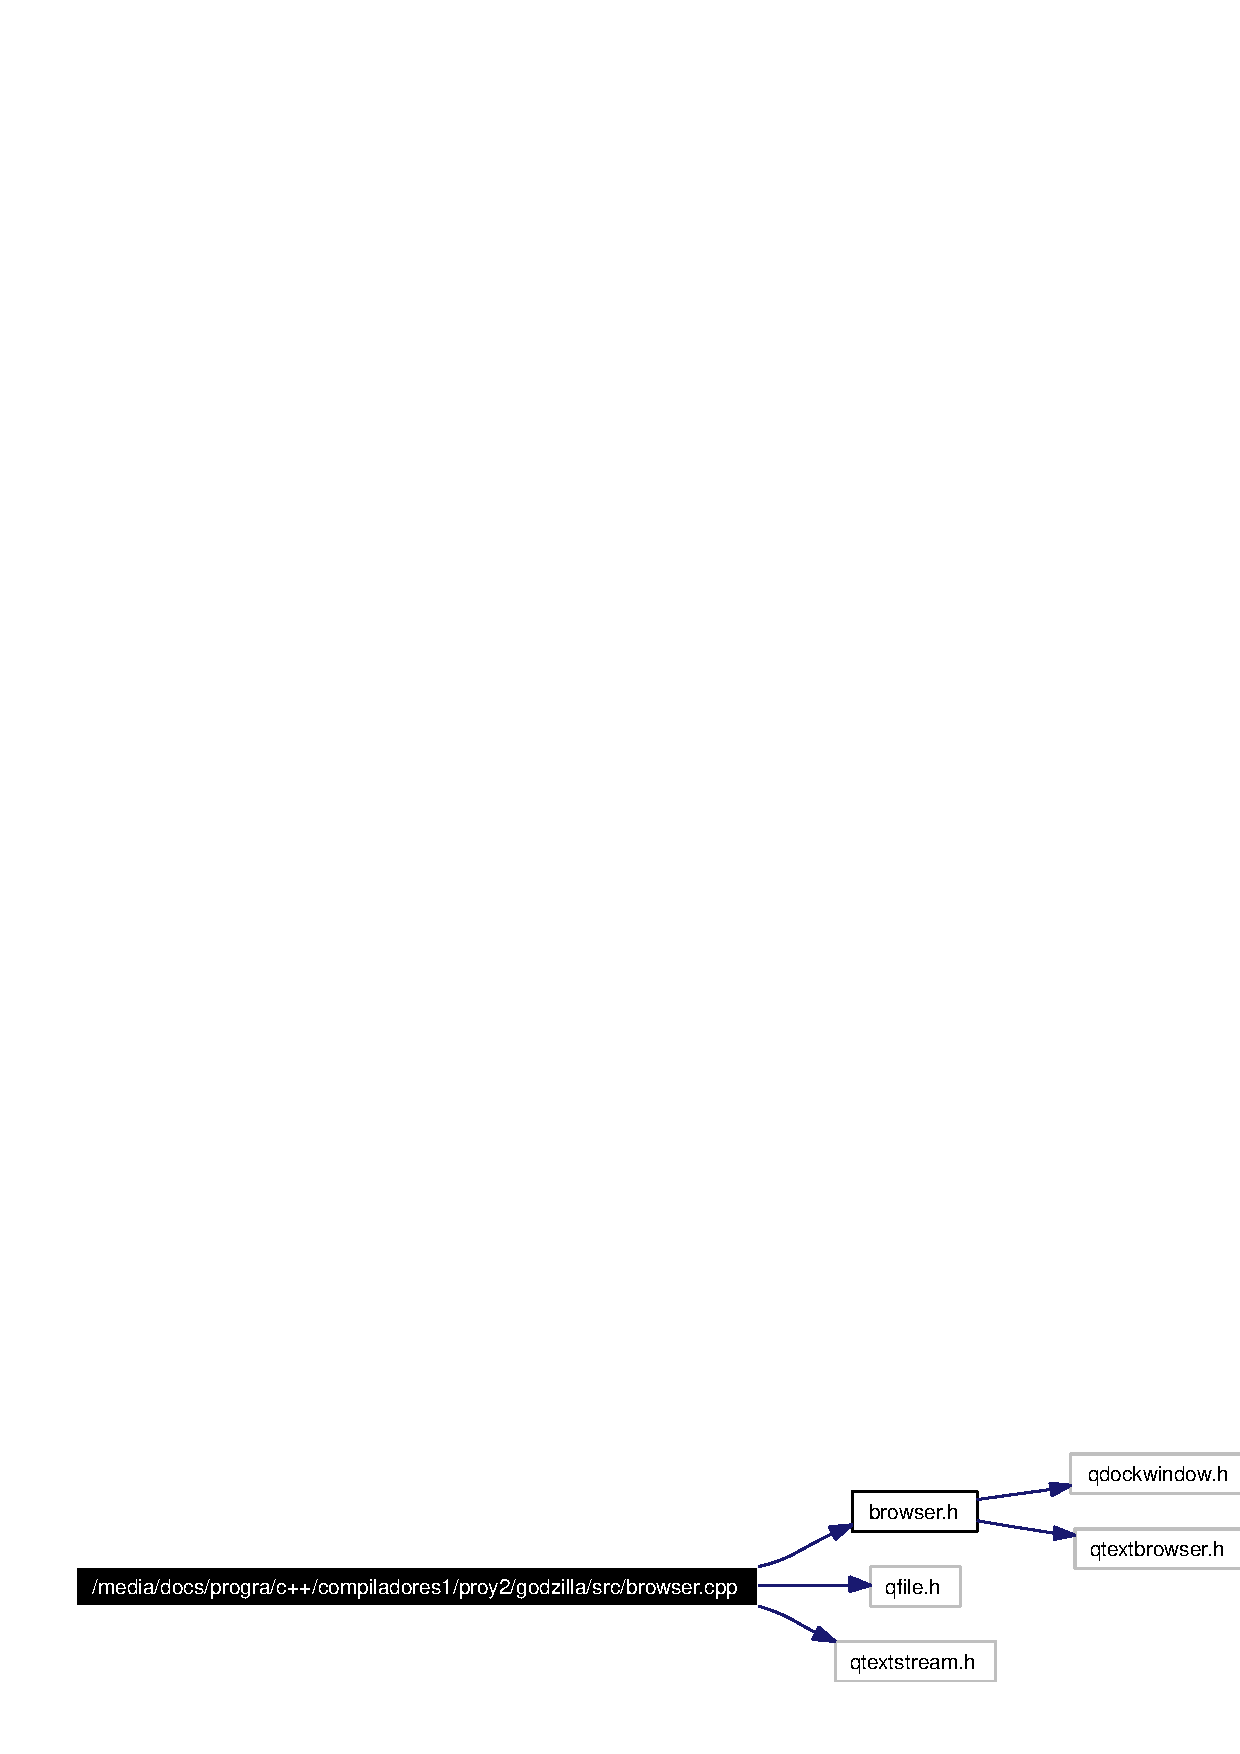
\includegraphics[width=299pt]{browser_8cpp__incl}
\end{center}
\end{figure}


\subsection{Descripci\'{o}n detallada}
Implementacion de la clase browser\-Dock. 



Definici\'{o}n en el archivo {\bf browser.cpp}.
\section{Referencia del Archivo /media/docs/progra/c++/compiladores1/proy2/godzilla/src/browser.h}
\label{browser_8h}\index{/media/docs/progra/c++/compiladores1/proy2/godzilla/src/browser.h@{/media/docs/progra/c++/compiladores1/proy2/godzilla/src/browser.h}}
Definiciones de la clase browser\-Dock. 

{\tt \#include $<$qdockwindow.h$>$}\par
{\tt \#include $<$qtextbrowser.h$>$}\par


Dependencia gr\'{a}fica adjunta para browser.h:\begin{figure}[H]
\begin{center}
\leavevmode
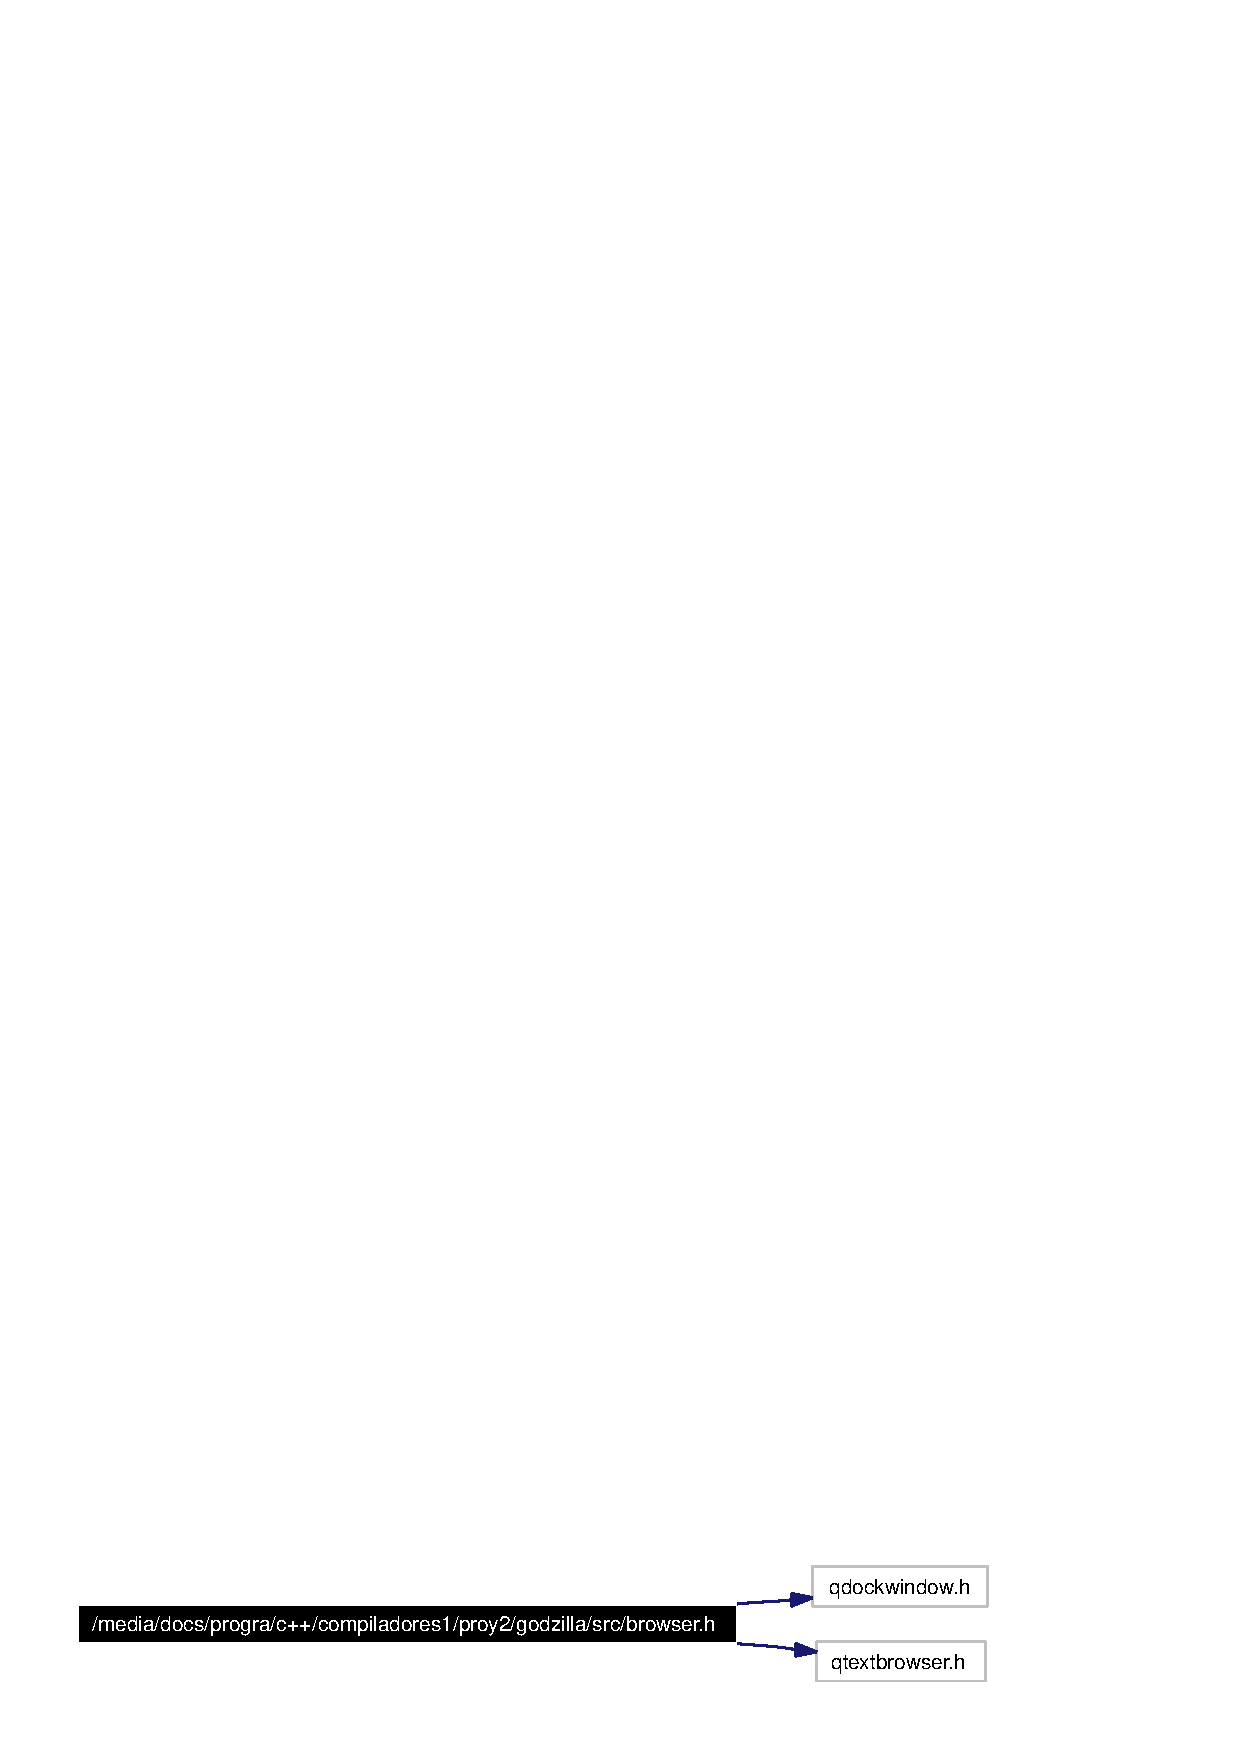
\includegraphics[width=237pt]{browser_8h__incl}
\end{center}
\end{figure}


Este gr\'{a}fico muestra que archivos directa o indirectamente incluyen a este archivo:\begin{figure}[H]
\begin{center}
\leavevmode
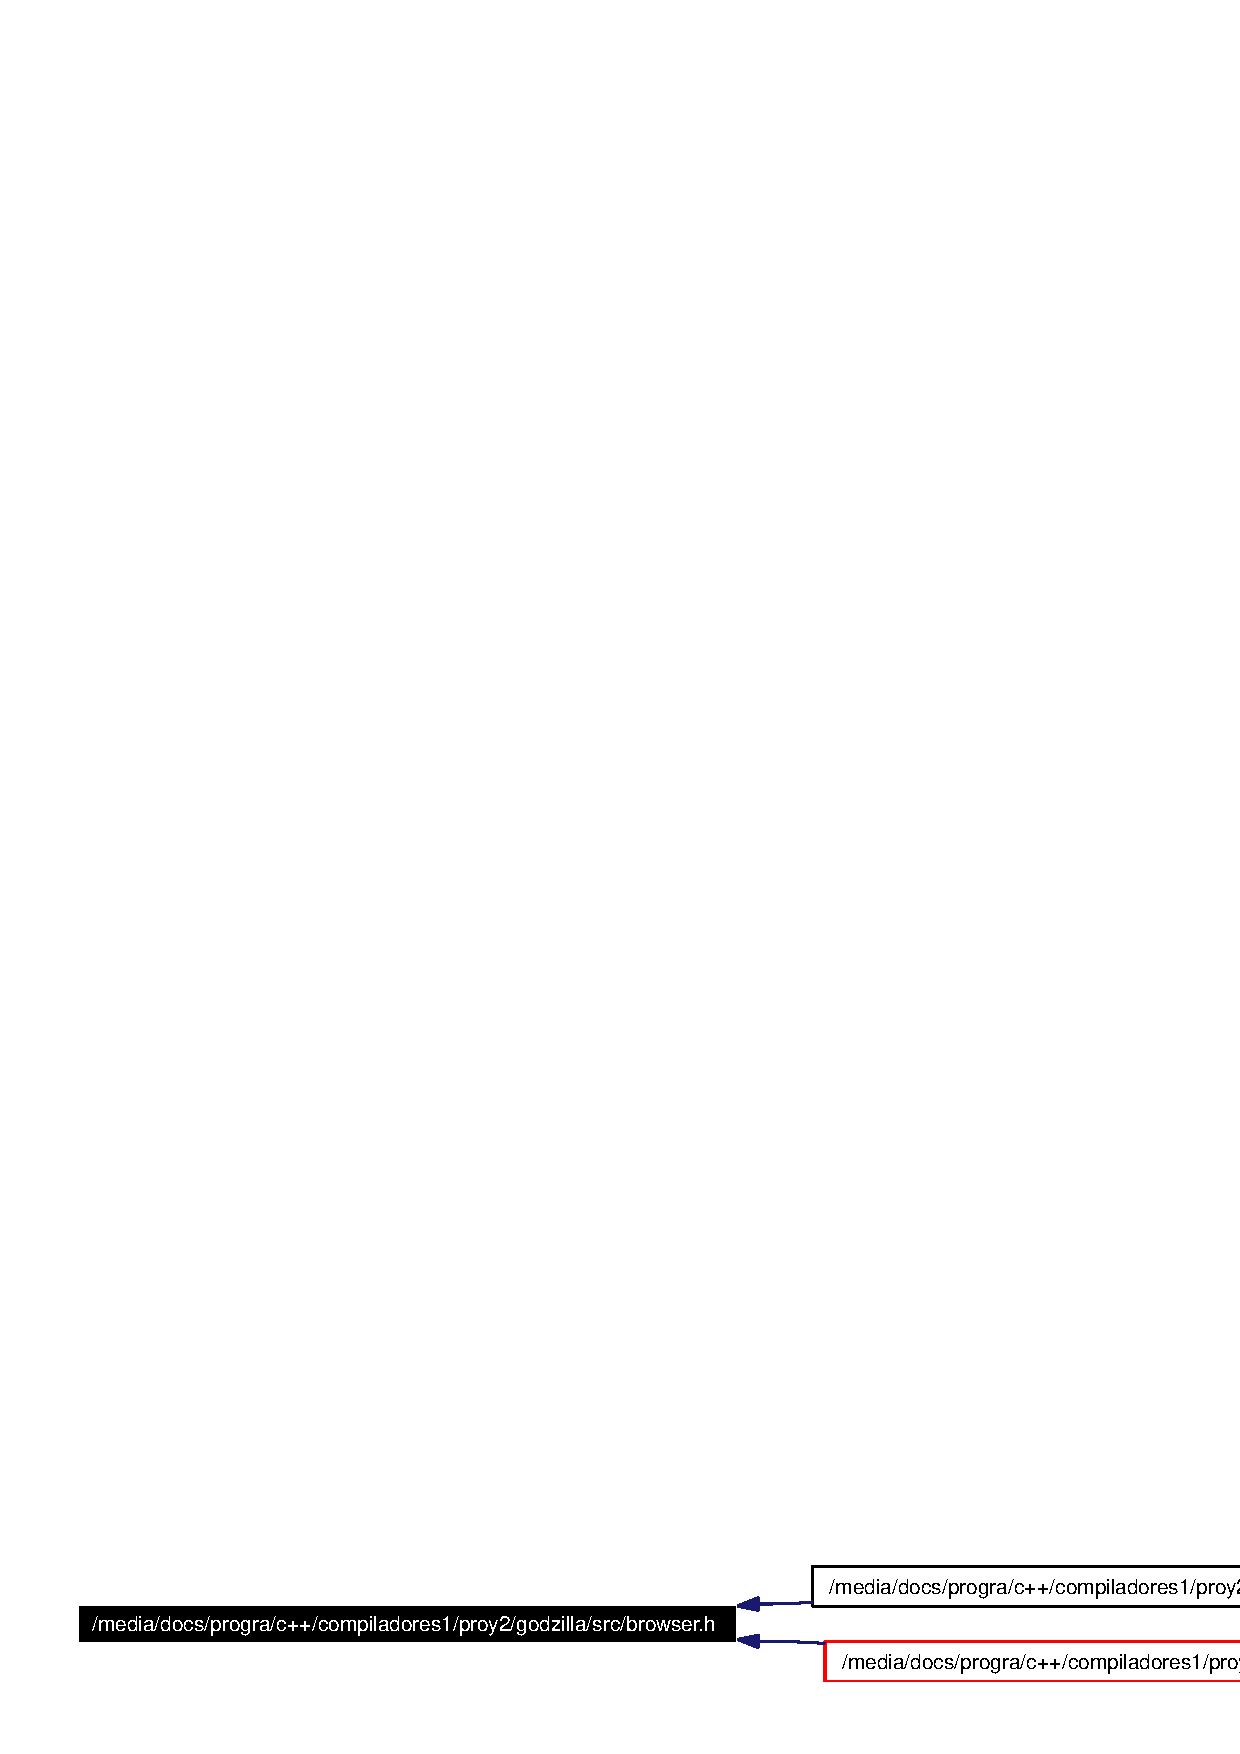
\includegraphics[width=359pt]{browser_8h__dep__incl}
\end{center}
\end{figure}
\subsection*{Clases}
\begin{CompactItemize}
\item 
class {\bf Browser\-Dock}
\begin{CompactList}\small\item\em Dock\-Window del browser empotrable en la ventana principal, heredando de QDock\-Window. \item\end{CompactList}\end{CompactItemize}


\subsection{Descripci\'{o}n detallada}
Definiciones de la clase browser\-Dock. 



Definici\'{o}n en el archivo {\bf browser.h}.
\section{Referencia del Archivo /media/docs/progra/c++/compiladores1/proy2/godzilla/src/colaerr.c}
\label{colaerr_8c}\index{/media/docs/progra/c++/compiladores1/proy2/godzilla/src/colaerr.c@{/media/docs/progra/c++/compiladores1/proy2/godzilla/src/colaerr.c}}
Implementacion de la cola almacenadora de errores . 

{\tt \#include \char`\"{}colaerr.h\char`\"{}}\par


Dependencia gr\'{a}fica adjunta para colaerr.c:\begin{figure}[H]
\begin{center}
\leavevmode
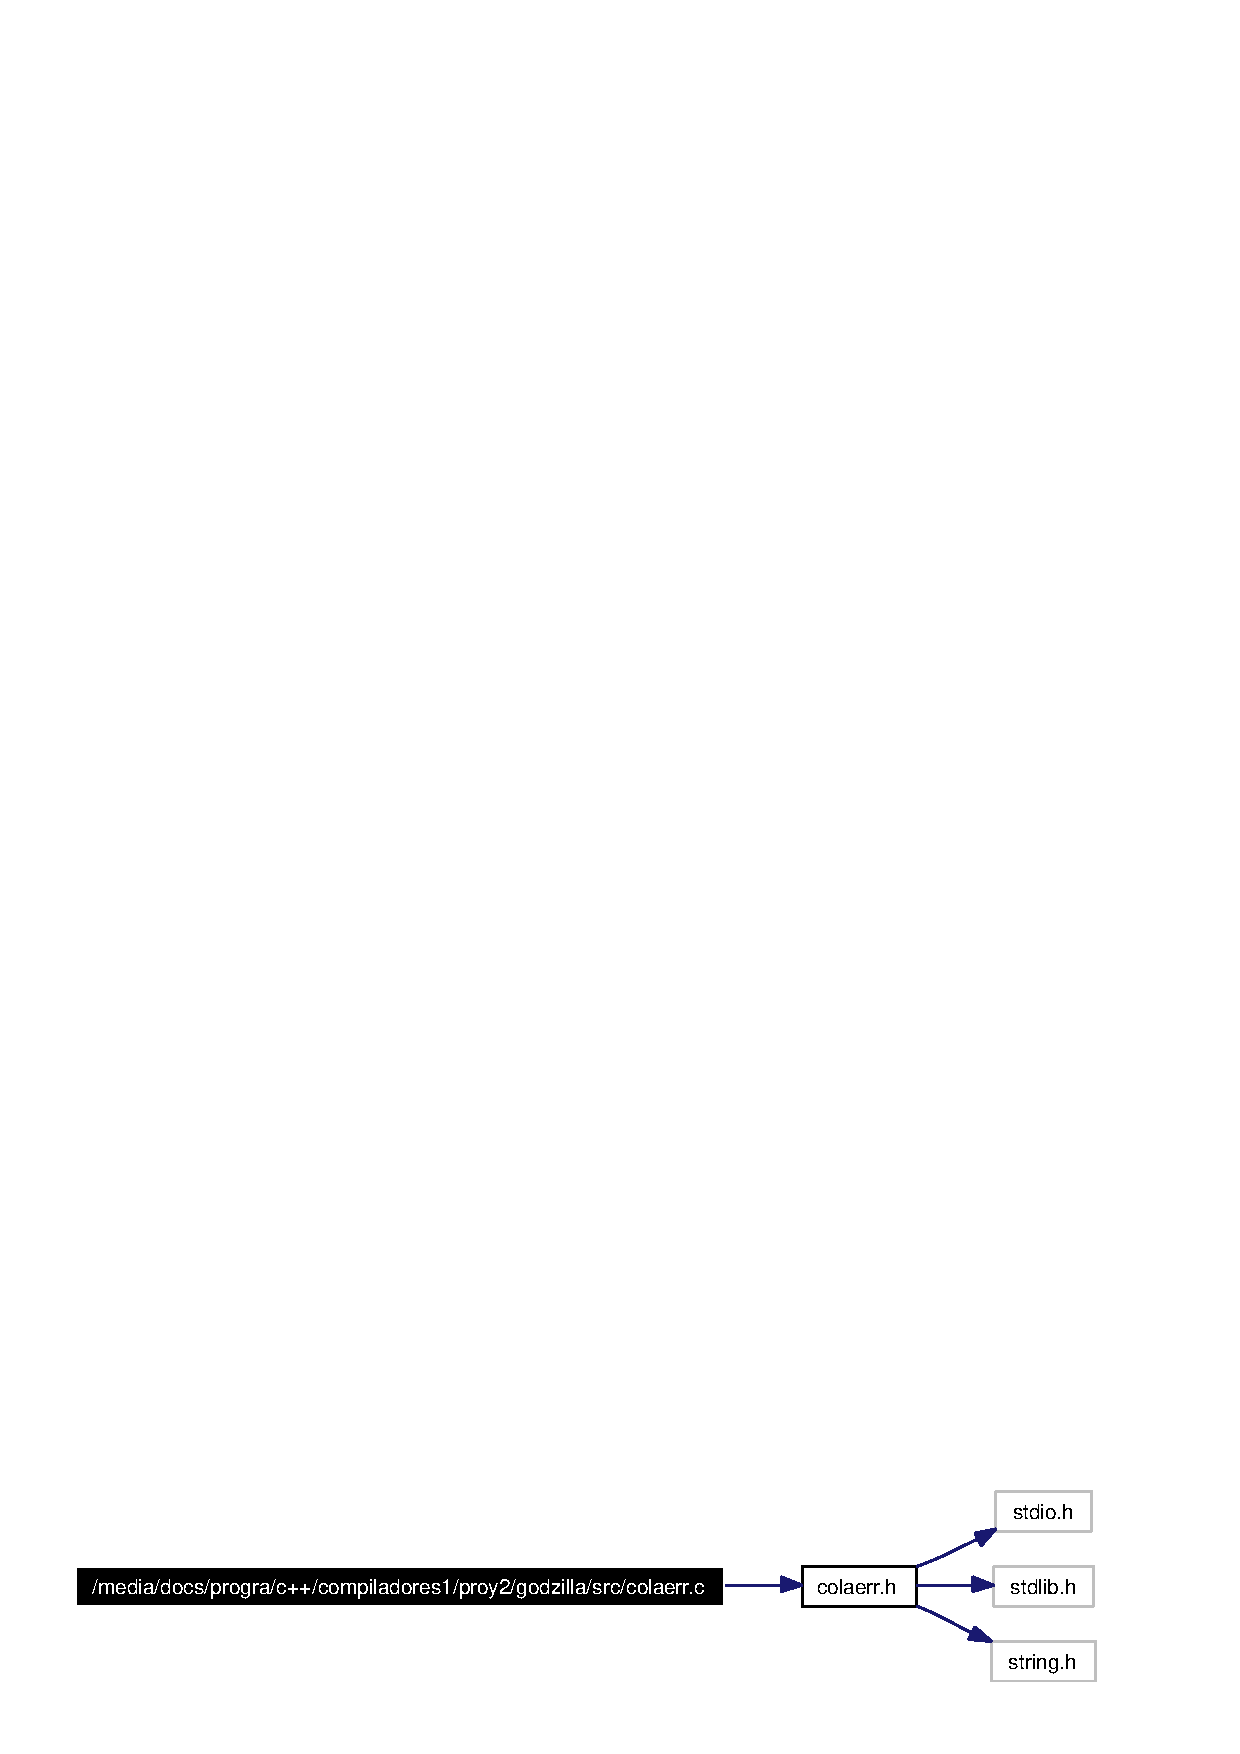
\includegraphics[width=263pt]{colaerr_8c__incl}
\end{center}
\end{figure}
\subsection*{Funciones}
\begin{CompactItemize}
\item 
void {\bf encolar\-Error} ({\bf cola\-Err} $\ast$cerr, {\bf tipo\-Error} $\ast$err)
\begin{CompactList}\small\item\em Agrega un error a la cola de errores. \item\end{CompactList}\item 
{\bf tipo\-Error} $\ast$ {\bf sacar\-Error} ({\bf cola\-Err} $\ast$cerr)
\begin{CompactList}\small\item\em Agrega un error a la cola de errores. \item\end{CompactList}\item 
void {\bf error\-Lexico} (char $\ast$msg)
\begin{CompactList}\small\item\em Devuelve primer error en la cola de erroes. \item\end{CompactList}\item 
void {\bf error\-Sintactico} (char $\ast$msg)
\begin{CompactList}\small\item\em Agrega mensaje a la cola de errores lexicos. \item\end{CompactList}\item 
void {\bf error\-Semantico} (char $\ast$msg, int num\-Linea)
\begin{CompactList}\small\item\em Agrega mensaje a la cola de errores sintacticos. \item\end{CompactList}\item 
int {\bf escribir\-Error\-Log\-XML} (const char $\ast$filename)
\begin{CompactList}\small\item\em Agrega mensaje a la cola de errores semanticos. \item\end{CompactList}\end{CompactItemize}
\subsection*{Variables}
\begin{CompactItemize}
\item 
static {\bf cola\-Err} {\bf errores\-Lexicos}
\item 
static {\bf cola\-Err} {\bf errores\-Sintacticos}
\item 
static {\bf cola\-Err} {\bf errores\-Semanticos}
\item 
static FILE $\ast$ {\bf errfile}
\item 
int {\bf hubo\-Error\-Sintactico} = 0
\item 
int {\bf hubo\-Error\-Semantico} = 0
\item 
int {\bf hubo\-Error\-Lexico} = 0
\end{CompactItemize}


\subsection{Descripci\'{o}n detallada}
Implementacion de la cola almacenadora de errores . 

Contiene rutinas de impresion hacia archivo XML 

Definici\'{o}n en el archivo {\bf colaerr.c}.

\subsection{Documentaci\'{o}n de las funciones}
\index{colaerr.c@{colaerr.c}!encolarError@{encolarError}}
\index{encolarError@{encolarError}!colaerr.c@{colaerr.c}}
\subsubsection{\setlength{\rightskip}{0pt plus 5cm}void encolar\-Error ({\bf cola\-Err} $\ast$ {\em cerr}, {\bf tipo\-Error} $\ast$ {\em err})}\label{colaerr_8c_a7}


Agrega un error a la cola de errores. 



Definici\'{o}n en la l\'{\i}nea 24 del archivo colaerr.c.

Hace referencia a nodo\-Cola\-Err::err, cola\-Err::primero, nodo\-Cola\-Err::siguiente, y cola\-Err::ultimo.

Referenciado por error\-Lexico(), error\-Semantico(), y error\-Sintactico().\index{colaerr.c@{colaerr.c}!errorLexico@{errorLexico}}
\index{errorLexico@{errorLexico}!colaerr.c@{colaerr.c}}
\subsubsection{\setlength{\rightskip}{0pt plus 5cm}void error\-Lexico (char $\ast$ {\em msg})}\label{colaerr_8c_a9}


Devuelve primer error en la cola de erroes. 



Definici\'{o}n en la l\'{\i}nea 53 del archivo colaerr.c.

Hace referencia a tipo\-Error::col, column, tipo\-Error::desc, encolar\-Error(), hubo\-Error\-Lexico, line\_\-num, y tipo\-Error::linea.\index{colaerr.c@{colaerr.c}!errorSemantico@{errorSemantico}}
\index{errorSemantico@{errorSemantico}!colaerr.c@{colaerr.c}}
\subsubsection{\setlength{\rightskip}{0pt plus 5cm}void error\-Semantico (char $\ast$ {\em msg}, int {\em num\-Linea})}\label{colaerr_8c_a11}


Agrega mensaje a la cola de errores sintacticos. 



Definici\'{o}n en la l\'{\i}nea 74 del archivo colaerr.c.

Hace referencia a tipo\-Error::col, tipo\-Error::desc, encolar\-Error(), hubo\-Error\-Semantico, y tipo\-Error::linea.

Referenciado por error().\index{colaerr.c@{colaerr.c}!errorSintactico@{errorSintactico}}
\index{errorSintactico@{errorSintactico}!colaerr.c@{colaerr.c}}
\subsubsection{\setlength{\rightskip}{0pt plus 5cm}void error\-Sintactico (char $\ast$ {\em msg})}\label{colaerr_8c_a10}


Agrega mensaje a la cola de errores lexicos. 



Definici\'{o}n en la l\'{\i}nea 63 del archivo colaerr.c.

Hace referencia a tipo\-Error::col, column, tipo\-Error::desc, encolar\-Error(), hubo\-Error\-Sintactico, line\_\-num, y tipo\-Error::linea.\index{colaerr.c@{colaerr.c}!escribirErrorLogXML@{escribirErrorLogXML}}
\index{escribirErrorLogXML@{escribirErrorLogXML}!colaerr.c@{colaerr.c}}
\subsubsection{\setlength{\rightskip}{0pt plus 5cm}int escribir\-Error\-Log\-XML (const char $\ast$ {\em filename})}\label{colaerr_8c_a12}


Agrega mensaje a la cola de errores semanticos. 



Definici\'{o}n en la l\'{\i}nea 84 del archivo colaerr.c.

Hace referencia a tipo\-Error::col, tipo\-Error::desc, errfile, tipo\-Error::linea, cola\-Err::primero, y sacar\-Error().\index{colaerr.c@{colaerr.c}!sacarError@{sacarError}}
\index{sacarError@{sacarError}!colaerr.c@{colaerr.c}}
\subsubsection{\setlength{\rightskip}{0pt plus 5cm}{\bf tipo\-Error}$\ast$ sacar\-Error ({\bf cola\-Err} $\ast$ {\em cerr})}\label{colaerr_8c_a8}


Agrega un error a la cola de errores. 



Definici\'{o}n en la l\'{\i}nea 36 del archivo colaerr.c.

Hace referencia a nodo\-Cola\-Err::err, cola\-Err::primero, nodo\-Cola\-Err::siguiente, y cola\-Err::ultimo.

Referenciado por escribir\-Error\-Log\-XML().

\subsection{Documentaci\'{o}n de las variables}
\index{colaerr.c@{colaerr.c}!errfile@{errfile}}
\index{errfile@{errfile}!colaerr.c@{colaerr.c}}
\subsubsection{\setlength{\rightskip}{0pt plus 5cm}FILE$\ast$ {\bf errfile}\hspace{0.3cm}{\tt  [static]}}\label{colaerr_8c_a3}




Definici\'{o}n en la l\'{\i}nea 17 del archivo colaerr.c.

Referenciado por escribir\-Error\-Log\-XML().\index{colaerr.c@{colaerr.c}!erroresLexicos@{erroresLexicos}}
\index{erroresLexicos@{erroresLexicos}!colaerr.c@{colaerr.c}}
\subsubsection{\setlength{\rightskip}{0pt plus 5cm}{\bf cola\-Err} {\bf errores\-Lexicos}\hspace{0.3cm}{\tt  [static]}}\label{colaerr_8c_a0}




Definici\'{o}n en la l\'{\i}nea 16 del archivo colaerr.c.\index{colaerr.c@{colaerr.c}!erroresSemanticos@{erroresSemanticos}}
\index{erroresSemanticos@{erroresSemanticos}!colaerr.c@{colaerr.c}}
\subsubsection{\setlength{\rightskip}{0pt plus 5cm}{\bf cola\-Err} {\bf errores\-Semanticos}\hspace{0.3cm}{\tt  [static]}}\label{colaerr_8c_a2}




Definici\'{o}n en la l\'{\i}nea 16 del archivo colaerr.c.\index{colaerr.c@{colaerr.c}!erroresSintacticos@{erroresSintacticos}}
\index{erroresSintacticos@{erroresSintacticos}!colaerr.c@{colaerr.c}}
\subsubsection{\setlength{\rightskip}{0pt plus 5cm}{\bf cola\-Err} {\bf errores\-Sintacticos}\hspace{0.3cm}{\tt  [static]}}\label{colaerr_8c_a1}




Definici\'{o}n en la l\'{\i}nea 16 del archivo colaerr.c.\index{colaerr.c@{colaerr.c}!huboErrorLexico@{huboErrorLexico}}
\index{huboErrorLexico@{huboErrorLexico}!colaerr.c@{colaerr.c}}
\subsubsection{\setlength{\rightskip}{0pt plus 5cm}int {\bf hubo\-Error\-Lexico} = 0}\label{colaerr_8c_a6}




Definici\'{o}n en la l\'{\i}nea 22 del archivo colaerr.c.

Referenciado por error\-Lexico().\index{colaerr.c@{colaerr.c}!huboErrorSemantico@{huboErrorSemantico}}
\index{huboErrorSemantico@{huboErrorSemantico}!colaerr.c@{colaerr.c}}
\subsubsection{\setlength{\rightskip}{0pt plus 5cm}int {\bf hubo\-Error\-Semantico} = 0}\label{colaerr_8c_a5}




Definici\'{o}n en la l\'{\i}nea 21 del archivo colaerr.c.

Referenciado por error\-Semantico().\index{colaerr.c@{colaerr.c}!huboErrorSintactico@{huboErrorSintactico}}
\index{huboErrorSintactico@{huboErrorSintactico}!colaerr.c@{colaerr.c}}
\subsubsection{\setlength{\rightskip}{0pt plus 5cm}int {\bf hubo\-Error\-Sintactico} = 0}\label{colaerr_8c_a4}




Definici\'{o}n en la l\'{\i}nea 20 del archivo colaerr.c.

Referenciado por error\-Sintactico().
\section{Referencia del Archivo /media/docs/progra/c++/compiladores1/proy2/godzilla/src/colaerr.h}
\label{colaerr_8h}\index{/media/docs/progra/c++/compiladores1/proy2/godzilla/src/colaerr.h@{/media/docs/progra/c++/compiladores1/proy2/godzilla/src/colaerr.h}}
Definiciones de la cola almacenadora de errores . 

{\tt \#include $<$stdio.h$>$}\par
{\tt \#include $<$stdlib.h$>$}\par
{\tt \#include $<$string.h$>$}\par


Dependencia gr\'{a}fica adjunta para colaerr.h:\begin{figure}[H]
\begin{center}
\leavevmode
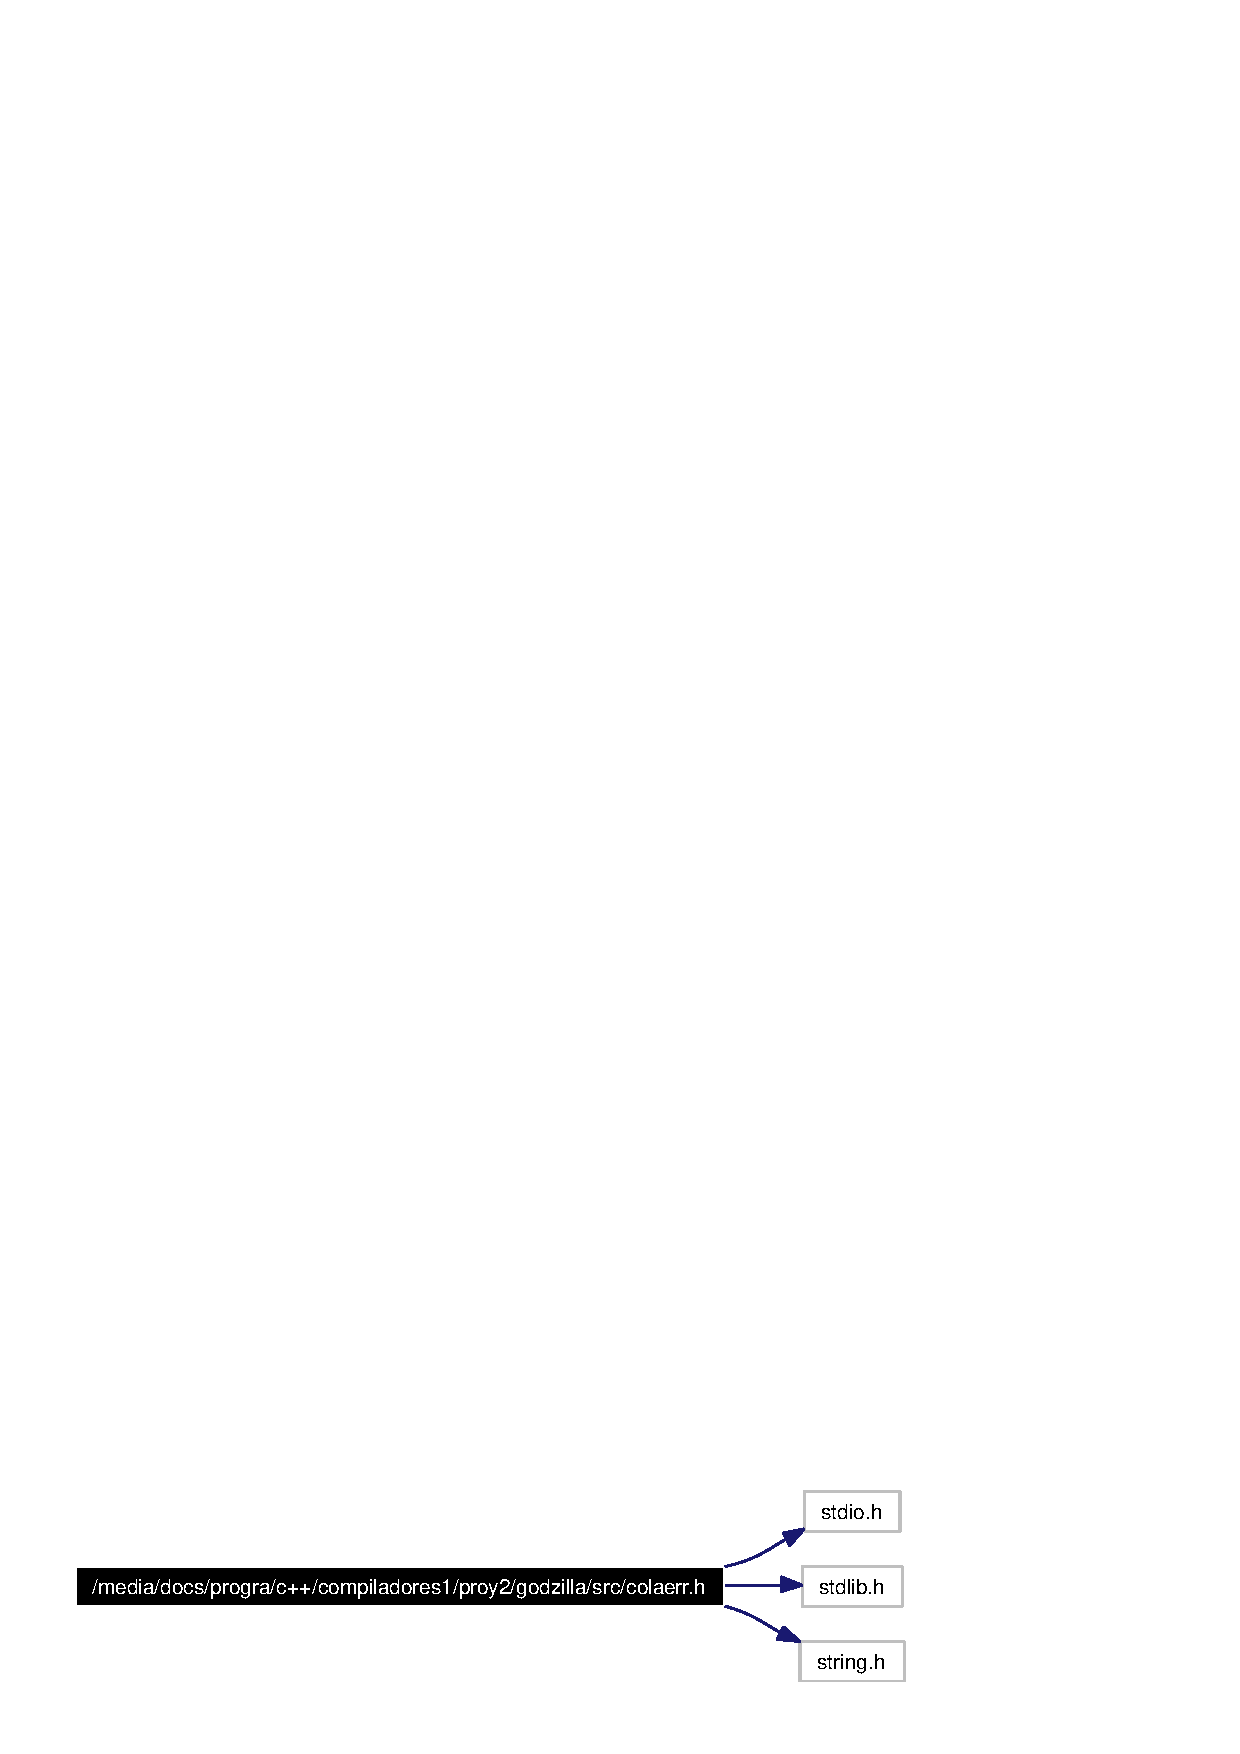
\includegraphics[width=217pt]{colaerr_8h__incl}
\end{center}
\end{figure}


Este gr\'{a}fico muestra que archivos directa o indirectamente incluyen a este archivo:\begin{figure}[H]
\begin{center}
\leavevmode
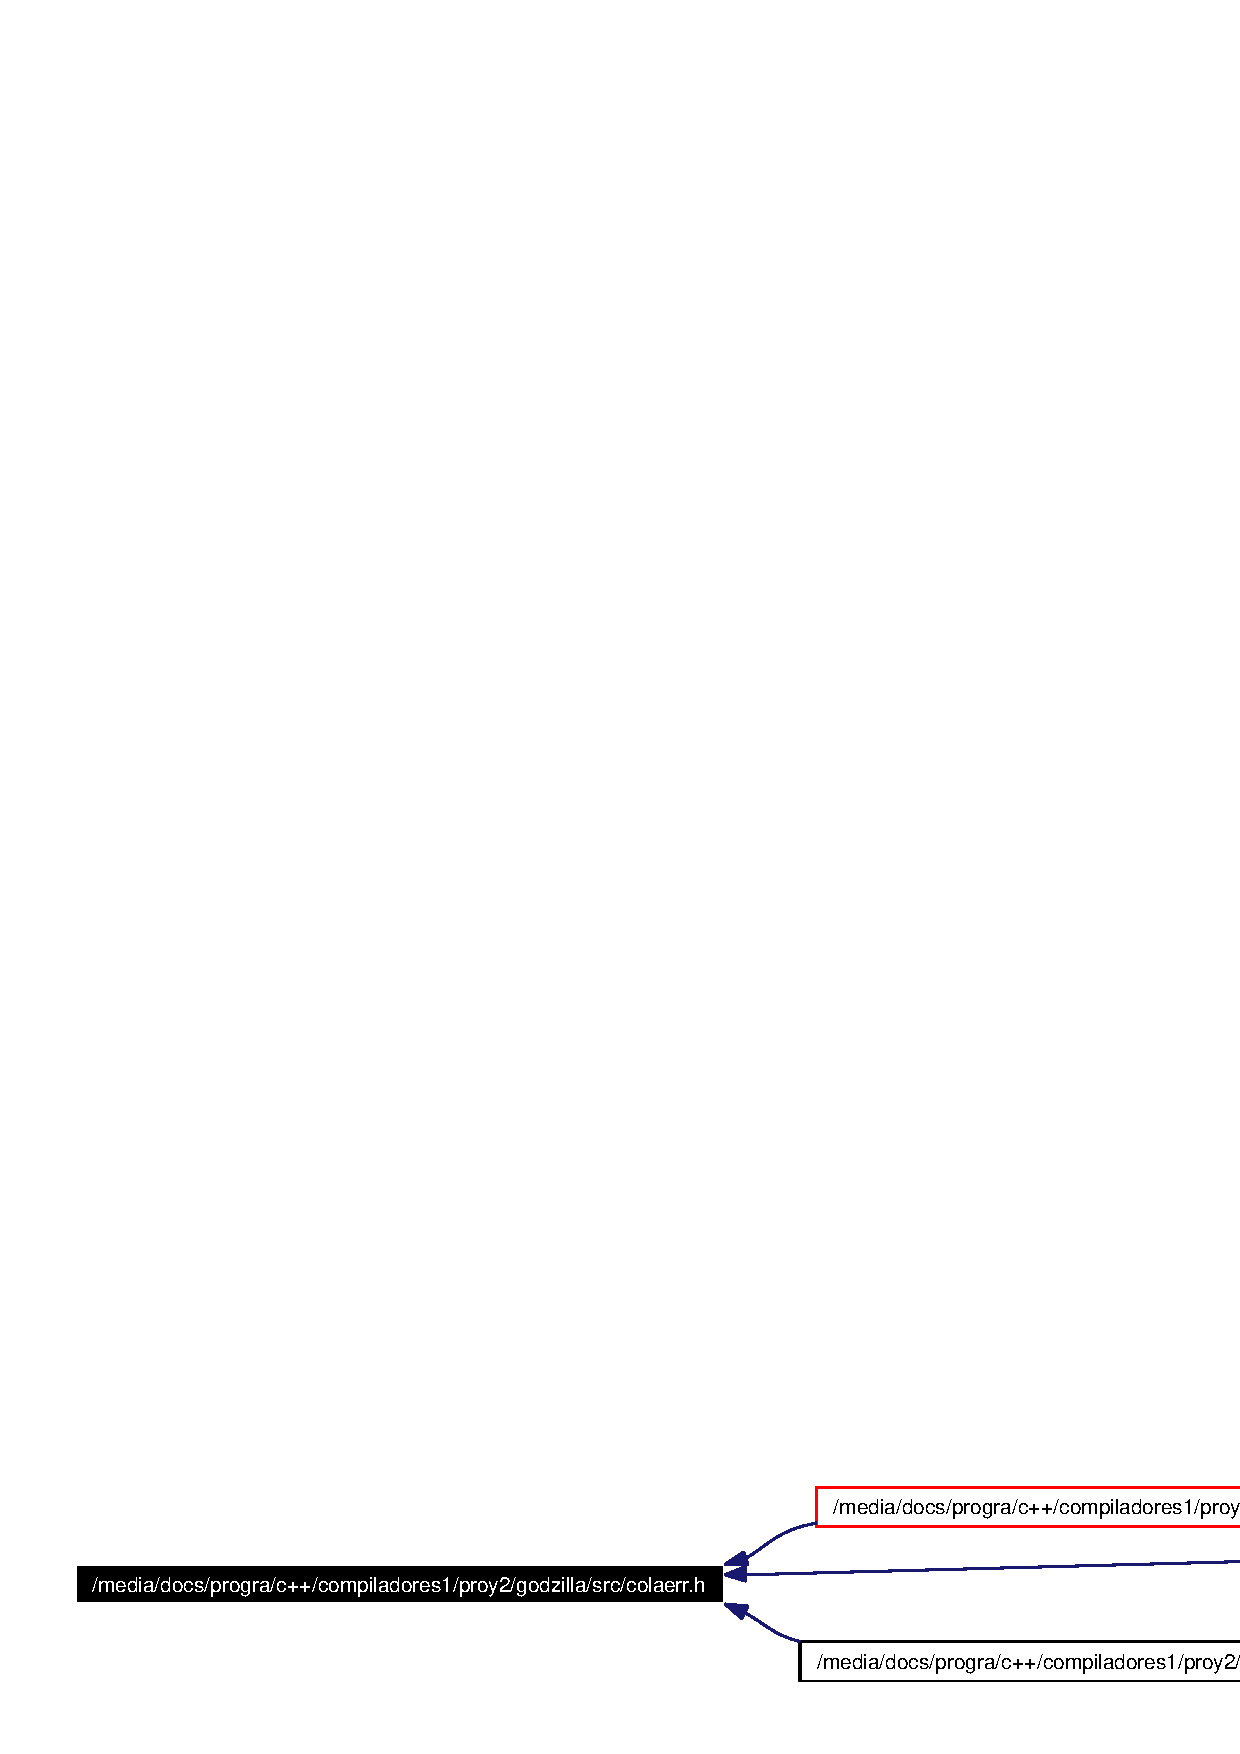
\includegraphics[width=420pt]{colaerr_8h__dep__incl}
\end{center}
\end{figure}
\subsection*{Clases}
\begin{CompactItemize}
\item 
struct {\bf tipo\-Error}
\begin{CompactList}\small\item\em Clase de almacenamiento de error. \item\end{CompactList}\item 
struct {\bf nodo\-Cola\-Err}
\begin{CompactList}\small\item\em Nodo de la cola de errores. \item\end{CompactList}\item 
struct {\bf cola\-Err}
\begin{CompactList}\small\item\em Cola de errores. \item\end{CompactList}\end{CompactItemize}
\subsection*{Tipos definidos}
\begin{CompactItemize}
\item 
typedef {\bf nodo\-Cola\-Err} {\bf nodo\-Cola\-Err}
\item 
typedef {\bf cola\-Err} {\bf cola\-Err}
\item 
typedef {\bf tipo\-Error} {\bf tipo\-Error}
\end{CompactItemize}
\subsection*{Funciones}
\begin{CompactItemize}
\item 
void {\bf encolar\-Error} ({\bf cola\-Err} $\ast$cerr, {\bf tipo\-Error} $\ast$err)
\begin{CompactList}\small\item\em Agrega un error a la cola de errores. \item\end{CompactList}\item 
{\bf tipo\-Error} $\ast$ {\bf sacar\-Error} ({\bf cola\-Err} $\ast$cerr)
\begin{CompactList}\small\item\em Agrega un error a la cola de errores. \item\end{CompactList}\item 
void {\bf error\-Lexico} (char $\ast$msg)
\begin{CompactList}\small\item\em Devuelve primer error en la cola de erroes. \item\end{CompactList}\item 
void {\bf error\-Sintactico} (char $\ast$msg)
\begin{CompactList}\small\item\em Agrega mensaje a la cola de errores lexicos. \item\end{CompactList}\item 
void {\bf error\-Semantico} (char $\ast$msg, int numlinea)
\begin{CompactList}\small\item\em Agrega mensaje a la cola de errores sintacticos. \item\end{CompactList}\item 
int {\bf escribir\-Error\-Log\-XML} (const char $\ast$filename)
\begin{CompactList}\small\item\em Agrega mensaje a la cola de errores semanticos. \item\end{CompactList}\end{CompactItemize}
\subsection*{Variables}
\begin{CompactItemize}
\item 
int {\bf line\_\-num}
\item 
int {\bf column}
\end{CompactItemize}


\subsection{Descripci\'{o}n detallada}
Definiciones de la cola almacenadora de errores . 



Definici\'{o}n en el archivo {\bf colaerr.h}.

\subsection{Documentaci\'{o}n de los tipos definidos}
\index{colaerr.h@{colaerr.h}!colaErr@{colaErr}}
\index{colaErr@{colaErr}!colaerr.h@{colaerr.h}}
\subsubsection{\setlength{\rightskip}{0pt plus 5cm}typedef struct {\bf cola\-Err} {\bf cola\-Err}}\label{colaerr_8h_a3}




Definici\'{o}n en la l\'{\i}nea 24 del archivo colaerr.h.\index{colaerr.h@{colaerr.h}!nodoColaErr@{nodoColaErr}}
\index{nodoColaErr@{nodoColaErr}!colaerr.h@{colaerr.h}}
\subsubsection{\setlength{\rightskip}{0pt plus 5cm}typedef struct {\bf nodo\-Cola\-Err} {\bf nodo\-Cola\-Err}}\label{colaerr_8h_a2}




Definici\'{o}n en la l\'{\i}nea 23 del archivo colaerr.h.\index{colaerr.h@{colaerr.h}!tipoError@{tipoError}}
\index{tipoError@{tipoError}!colaerr.h@{colaerr.h}}
\subsubsection{\setlength{\rightskip}{0pt plus 5cm}typedef struct {\bf tipo\-Error} {\bf tipo\-Error}}\label{colaerr_8h_a4}




Definici\'{o}n en la l\'{\i}nea 25 del archivo colaerr.h.

\subsection{Documentaci\'{o}n de las funciones}
\index{colaerr.h@{colaerr.h}!encolarError@{encolarError}}
\index{encolarError@{encolarError}!colaerr.h@{colaerr.h}}
\subsubsection{\setlength{\rightskip}{0pt plus 5cm}void encolar\-Error ({\bf cola\-Err} $\ast$ {\em cerr}, {\bf tipo\-Error} $\ast$ {\em err})}\label{colaerr_8h_a5}


Agrega un error a la cola de errores. 



Definici\'{o}n en la l\'{\i}nea 24 del archivo colaerr.c.

Hace referencia a nodo\-Cola\-Err::err, cola\-Err::primero, nodo\-Cola\-Err::siguiente, y cola\-Err::ultimo.

Referenciado por error\-Lexico(), error\-Semantico(), y error\-Sintactico().\index{colaerr.h@{colaerr.h}!errorLexico@{errorLexico}}
\index{errorLexico@{errorLexico}!colaerr.h@{colaerr.h}}
\subsubsection{\setlength{\rightskip}{0pt plus 5cm}void error\-Lexico (char $\ast$ {\em msg})}\label{colaerr_8h_a7}


Devuelve primer error en la cola de erroes. 



Definici\'{o}n en la l\'{\i}nea 53 del archivo colaerr.c.

Hace referencia a tipo\-Error::col, column, tipo\-Error::desc, encolar\-Error(), hubo\-Error\-Lexico, line\_\-num, y tipo\-Error::linea.\index{colaerr.h@{colaerr.h}!errorSemantico@{errorSemantico}}
\index{errorSemantico@{errorSemantico}!colaerr.h@{colaerr.h}}
\subsubsection{\setlength{\rightskip}{0pt plus 5cm}void error\-Semantico (char $\ast$ {\em msg}, int {\em numlinea})}\label{colaerr_8h_a9}


Agrega mensaje a la cola de errores sintacticos. 



Definici\'{o}n en la l\'{\i}nea 74 del archivo colaerr.c.

Hace referencia a tipo\-Error::col, tipo\-Error::desc, encolar\-Error(), hubo\-Error\-Semantico, y tipo\-Error::linea.

Referenciado por error().\index{colaerr.h@{colaerr.h}!errorSintactico@{errorSintactico}}
\index{errorSintactico@{errorSintactico}!colaerr.h@{colaerr.h}}
\subsubsection{\setlength{\rightskip}{0pt plus 5cm}void error\-Sintactico (char $\ast$ {\em msg})}\label{colaerr_8h_a8}


Agrega mensaje a la cola de errores lexicos. 



Definici\'{o}n en la l\'{\i}nea 63 del archivo colaerr.c.

Hace referencia a tipo\-Error::col, column, tipo\-Error::desc, encolar\-Error(), hubo\-Error\-Sintactico, line\_\-num, y tipo\-Error::linea.\index{colaerr.h@{colaerr.h}!escribirErrorLogXML@{escribirErrorLogXML}}
\index{escribirErrorLogXML@{escribirErrorLogXML}!colaerr.h@{colaerr.h}}
\subsubsection{\setlength{\rightskip}{0pt plus 5cm}int escribir\-Error\-Log\-XML (const char $\ast$ {\em filename})}\label{colaerr_8h_a10}


Agrega mensaje a la cola de errores semanticos. 



Definici\'{o}n en la l\'{\i}nea 84 del archivo colaerr.c.

Hace referencia a tipo\-Error::col, tipo\-Error::desc, errfile, tipo\-Error::linea, cola\-Err::primero, y sacar\-Error().\index{colaerr.h@{colaerr.h}!sacarError@{sacarError}}
\index{sacarError@{sacarError}!colaerr.h@{colaerr.h}}
\subsubsection{\setlength{\rightskip}{0pt plus 5cm}{\bf tipo\-Error}$\ast$ sacar\-Error ({\bf cola\-Err} $\ast$ {\em cerr})}\label{colaerr_8h_a6}


Agrega un error a la cola de errores. 



Definici\'{o}n en la l\'{\i}nea 36 del archivo colaerr.c.

Hace referencia a nodo\-Cola\-Err::err, cola\-Err::primero, nodo\-Cola\-Err::siguiente, y cola\-Err::ultimo.

Referenciado por escribir\-Error\-Log\-XML().

\subsection{Documentaci\'{o}n de las variables}
\index{colaerr.h@{colaerr.h}!column@{column}}
\index{column@{column}!colaerr.h@{colaerr.h}}
\subsubsection{\setlength{\rightskip}{0pt plus 5cm}int {\bf column}}\label{colaerr_8h_a1}




Referenciado por error\-Lexico(), y error\-Sintactico().\index{colaerr.h@{colaerr.h}!line_num@{line\_\-num}}
\index{line_num@{line\_\-num}!colaerr.h@{colaerr.h}}
\subsubsection{\setlength{\rightskip}{0pt plus 5cm}int {\bf line\_\-num}}\label{colaerr_8h_a0}




Referenciado por error\-Lexico(), y error\-Sintactico().
\section{Referencia del Archivo /media/docs/progra/c++/compiladores1/proy2/godzilla/src/constantes.h}
\label{constantes_8h}\index{/media/docs/progra/c++/compiladores1/proy2/godzilla/src/constantes.h@{/media/docs/progra/c++/compiladores1/proy2/godzilla/src/constantes.h}}
Constantes utilizadas por el arbol de sintaxis abstracta. 



Este gr\'{a}fico muestra que archivos directa o indirectamente incluyen a este archivo:\begin{figure}[H]
\begin{center}
\leavevmode
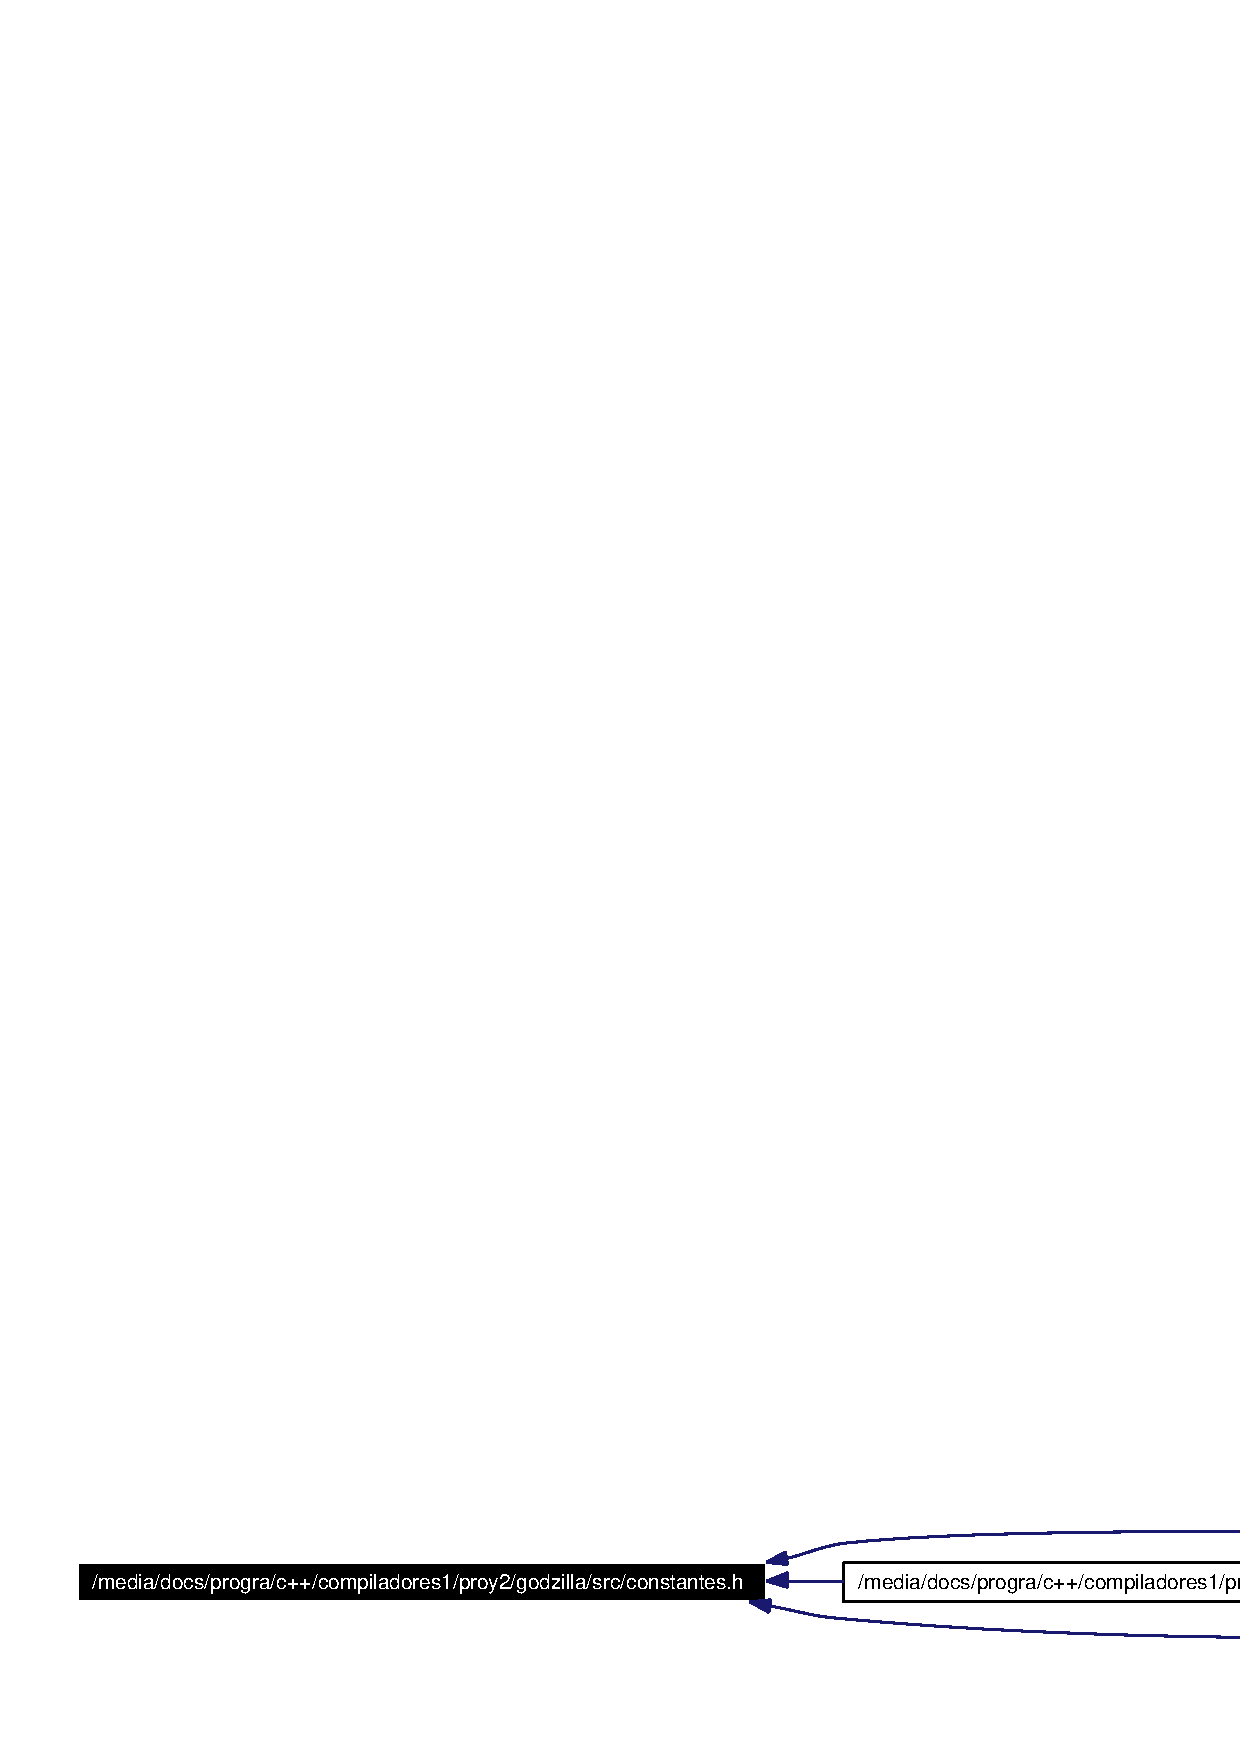
\includegraphics[width=420pt]{constantes_8h__dep__incl}
\end{center}
\end{figure}
\subsection*{Definiciones}
\begin{CompactItemize}
\item 
\#define {\bf T\_\-ERROR}~-1
\item 
\#define {\bf T\_\-FALSE}~0
\item 
\#define {\bf T\_\-TRUE}~1
\item 
\#define {\bf T\_\-CONSTANTE}~1000
\item 
\#define {\bf T\_\-VARIABLE}~1001
\item 
\#define {\bf T\_\-NUMERO}~1002
\item 
\#define {\bf T\_\-IDENTIFICADOR}~1003
\item 
\#define {\bf T\_\-OPERACION}~1004
\item 
\#define {\bf T\_\-EXPR}~1005
\item 
\#define {\bf T\_\-ASIGNACION}~1006
\item 
\#define {\bf T\_\-SENTENCIA}~1007
\item 
\#define {\bf T\_\-DECLARACION}~1008
\item 
\#define {\bf T\_\-IF}~1009
\item 
\#define {\bf T\_\-WHILE}~1010
\item 
\#define {\bf T\_\-FOR}~1011
\item 
\#define {\bf T\_\-TOKEN}~1012
\item 
\#define {\bf T\_\-CALL}~1013
\item 
\#define {\bf T\_\-CADENA}~1015
\item 
\#define {\bf OP\_\-OR}~1016
\item 
\#define {\bf OP\_\-AND}~1017
\item 
\#define {\bf OP\_\-LT}~1018
\item 
\#define {\bf OP\_\-LET}~1019
\item 
\#define {\bf OP\_\-EQ}~1020
\item 
\#define {\bf OP\_\-NEQ}~1021
\item 
\#define {\bf OP\_\-GT}~1022
\item 
\#define {\bf OP\_\-GET}~1023
\item 
\#define {\bf OP\_\-SUMA}~1024
\item 
\#define {\bf OP\_\-RESTA}~1025
\item 
\#define {\bf OP\_\-MULT}~1026
\item 
\#define {\bf OP\_\-DIV}~1027
\item 
\#define {\bf T\_\-INTEGER}~1028
\item 
\#define {\bf T\_\-BOOLEAN}~1029
\item 
\#define {\bf T\_\-STRING}~1030
\item 
\#define {\bf T\_\-LITERAL}~1031
\item 
\#define {\bf T\_\-PRINTCALL}~1032
\item 
\#define {\bf T\_\-PRINTSYMCALL}~1033
\end{CompactItemize}


\subsection{Descripci\'{o}n detallada}
Constantes utilizadas por el arbol de sintaxis abstracta. 



Definici\'{o}n en el archivo {\bf constantes.h}.

\subsection{Documentaci\'{o}n de las definiciones}
\index{constantes.h@{constantes.h}!OP_AND@{OP\_\-AND}}
\index{OP_AND@{OP\_\-AND}!constantes.h@{constantes.h}}
\subsubsection{\setlength{\rightskip}{0pt plus 5cm}\#define OP\_\-AND~1017}\label{constantes_8h_a19}




Definici\'{o}n en la l\'{\i}nea 30 del archivo constantes.h.

Referenciado por evaluar\-Operacion().\index{constantes.h@{constantes.h}!OP_DIV@{OP\_\-DIV}}
\index{OP_DIV@{OP\_\-DIV}!constantes.h@{constantes.h}}
\subsubsection{\setlength{\rightskip}{0pt plus 5cm}\#define OP\_\-DIV~1027}\label{constantes_8h_a29}




Definici\'{o}n en la l\'{\i}nea 40 del archivo constantes.h.

Referenciado por evaluar\-Operacion().\index{constantes.h@{constantes.h}!OP_EQ@{OP\_\-EQ}}
\index{OP_EQ@{OP\_\-EQ}!constantes.h@{constantes.h}}
\subsubsection{\setlength{\rightskip}{0pt plus 5cm}\#define OP\_\-EQ~1020}\label{constantes_8h_a22}




Definici\'{o}n en la l\'{\i}nea 33 del archivo constantes.h.

Referenciado por evaluar\-Operacion().\index{constantes.h@{constantes.h}!OP_GET@{OP\_\-GET}}
\index{OP_GET@{OP\_\-GET}!constantes.h@{constantes.h}}
\subsubsection{\setlength{\rightskip}{0pt plus 5cm}\#define OP\_\-GET~1023}\label{constantes_8h_a25}




Definici\'{o}n en la l\'{\i}nea 36 del archivo constantes.h.

Referenciado por evaluar\-Operacion().\index{constantes.h@{constantes.h}!OP_GT@{OP\_\-GT}}
\index{OP_GT@{OP\_\-GT}!constantes.h@{constantes.h}}
\subsubsection{\setlength{\rightskip}{0pt plus 5cm}\#define OP\_\-GT~1022}\label{constantes_8h_a24}




Definici\'{o}n en la l\'{\i}nea 35 del archivo constantes.h.

Referenciado por evaluar\-Operacion().\index{constantes.h@{constantes.h}!OP_LET@{OP\_\-LET}}
\index{OP_LET@{OP\_\-LET}!constantes.h@{constantes.h}}
\subsubsection{\setlength{\rightskip}{0pt plus 5cm}\#define OP\_\-LET~1019}\label{constantes_8h_a21}




Definici\'{o}n en la l\'{\i}nea 32 del archivo constantes.h.

Referenciado por evaluar\-Operacion().\index{constantes.h@{constantes.h}!OP_LT@{OP\_\-LT}}
\index{OP_LT@{OP\_\-LT}!constantes.h@{constantes.h}}
\subsubsection{\setlength{\rightskip}{0pt plus 5cm}\#define OP\_\-LT~1018}\label{constantes_8h_a20}




Definici\'{o}n en la l\'{\i}nea 31 del archivo constantes.h.

Referenciado por evaluar\-Operacion().\index{constantes.h@{constantes.h}!OP_MULT@{OP\_\-MULT}}
\index{OP_MULT@{OP\_\-MULT}!constantes.h@{constantes.h}}
\subsubsection{\setlength{\rightskip}{0pt plus 5cm}\#define OP\_\-MULT~1026}\label{constantes_8h_a28}




Definici\'{o}n en la l\'{\i}nea 39 del archivo constantes.h.

Referenciado por evaluar\-Operacion().\index{constantes.h@{constantes.h}!OP_NEQ@{OP\_\-NEQ}}
\index{OP_NEQ@{OP\_\-NEQ}!constantes.h@{constantes.h}}
\subsubsection{\setlength{\rightskip}{0pt plus 5cm}\#define OP\_\-NEQ~1021}\label{constantes_8h_a23}




Definici\'{o}n en la l\'{\i}nea 34 del archivo constantes.h.

Referenciado por evaluar\-Operacion().\index{constantes.h@{constantes.h}!OP_OR@{OP\_\-OR}}
\index{OP_OR@{OP\_\-OR}!constantes.h@{constantes.h}}
\subsubsection{\setlength{\rightskip}{0pt plus 5cm}\#define OP\_\-OR~1016}\label{constantes_8h_a18}




Definici\'{o}n en la l\'{\i}nea 29 del archivo constantes.h.

Referenciado por evaluar\-Operacion().\index{constantes.h@{constantes.h}!OP_RESTA@{OP\_\-RESTA}}
\index{OP_RESTA@{OP\_\-RESTA}!constantes.h@{constantes.h}}
\subsubsection{\setlength{\rightskip}{0pt plus 5cm}\#define OP\_\-RESTA~1025}\label{constantes_8h_a27}




Definici\'{o}n en la l\'{\i}nea 38 del archivo constantes.h.

Referenciado por evaluar\-Operacion().\index{constantes.h@{constantes.h}!OP_SUMA@{OP\_\-SUMA}}
\index{OP_SUMA@{OP\_\-SUMA}!constantes.h@{constantes.h}}
\subsubsection{\setlength{\rightskip}{0pt plus 5cm}\#define OP\_\-SUMA~1024}\label{constantes_8h_a26}




Definici\'{o}n en la l\'{\i}nea 37 del archivo constantes.h.

Referenciado por evaluar\-Operacion().\index{constantes.h@{constantes.h}!T_ASIGNACION@{T\_\-ASIGNACION}}
\index{T_ASIGNACION@{T\_\-ASIGNACION}!constantes.h@{constantes.h}}
\subsubsection{\setlength{\rightskip}{0pt plus 5cm}\#define T\_\-ASIGNACION~1006}\label{constantes_8h_a9}




Definici\'{o}n en la l\'{\i}nea 20 del archivo constantes.h.

Referenciado por borrar\-Sentencias(), evaluar\-Asignacion(), evaluar\-Sentencia(), insertar\-Asignacion(), y insertar\-Sentencia().\index{constantes.h@{constantes.h}!T_BOOLEAN@{T\_\-BOOLEAN}}
\index{T_BOOLEAN@{T\_\-BOOLEAN}!constantes.h@{constantes.h}}
\subsubsection{\setlength{\rightskip}{0pt plus 5cm}\#define T\_\-BOOLEAN~1029}\label{constantes_8h_a31}




Definici\'{o}n en la l\'{\i}nea 42 del archivo constantes.h.

Referenciado por evaluar\-And(), evaluar\-Asignacion(), evaluar\-EQ(), evaluar\-Expresion(), evaluar\-GET(), evaluar\-GT(), evaluar\-If(), evaluar\-LET(), evaluar\-LT(), evaluar\-NEQ(), evaluar\-Or(), evaluar\-While(), imprimir\-Tokens(), insertar\-Simbolo(), y print\-Symtab\-File().\index{constantes.h@{constantes.h}!T_CADENA@{T\_\-CADENA}}
\index{T_CADENA@{T\_\-CADENA}!constantes.h@{constantes.h}}
\subsubsection{\setlength{\rightskip}{0pt plus 5cm}\#define T\_\-CADENA~1015}\label{constantes_8h_a17}




Definici\'{o}n en la l\'{\i}nea 28 del archivo constantes.h.

Referenciado por borrar\-Tokens(), imprimir\-Tokens(), y insertar\-Token().\index{constantes.h@{constantes.h}!T_CALL@{T\_\-CALL}}
\index{T_CALL@{T\_\-CALL}!constantes.h@{constantes.h}}
\subsubsection{\setlength{\rightskip}{0pt plus 5cm}\#define T\_\-CALL~1013}\label{constantes_8h_a16}




Definici\'{o}n en la l\'{\i}nea 27 del archivo constantes.h.

Referenciado por borrar\-Sentencias(), evaluar\-Print\-Call(), evaluar\-Sentencia(), insertar\-Llamada(), insertar\-Llamada\-Sym\-Tab(), y insertar\-Sentencia().\index{constantes.h@{constantes.h}!T_CONSTANTE@{T\_\-CONSTANTE}}
\index{T_CONSTANTE@{T\_\-CONSTANTE}!constantes.h@{constantes.h}}
\subsubsection{\setlength{\rightskip}{0pt plus 5cm}\#define T\_\-CONSTANTE~1000}\label{constantes_8h_a3}




Definici\'{o}n en la l\'{\i}nea 14 del archivo constantes.h.

Referenciado por borrar\-Expresion(), evaluar\-Expresion(), insertar\-Constante(), y insertar\-Expresion().\index{constantes.h@{constantes.h}!T_DECLARACION@{T\_\-DECLARACION}}
\index{T_DECLARACION@{T\_\-DECLARACION}!constantes.h@{constantes.h}}
\subsubsection{\setlength{\rightskip}{0pt plus 5cm}\#define T\_\-DECLARACION~1008}\label{constantes_8h_a11}




Definici\'{o}n en la l\'{\i}nea 22 del archivo constantes.h.

Referenciado por borrar\-Sentencias(), evaluar\-Declaracion(), evaluar\-Sentencia(), insertar\-Declaracion(), y insertar\-Sentencia().\index{constantes.h@{constantes.h}!T_ERROR@{T\_\-ERROR}}
\index{T_ERROR@{T\_\-ERROR}!constantes.h@{constantes.h}}
\subsubsection{\setlength{\rightskip}{0pt plus 5cm}\#define T\_\-ERROR~-1}\label{constantes_8h_a0}




Definici\'{o}n en la l\'{\i}nea 11 del archivo constantes.h.

Referenciado por evaluar\-Sentencia(), y insertar\-Sentencia().\index{constantes.h@{constantes.h}!T_EXPR@{T\_\-EXPR}}
\index{T_EXPR@{T\_\-EXPR}!constantes.h@{constantes.h}}
\subsubsection{\setlength{\rightskip}{0pt plus 5cm}\#define T\_\-EXPR~1005}\label{constantes_8h_a8}




Definici\'{o}n en la l\'{\i}nea 19 del archivo constantes.h.

Referenciado por evaluar\-Expresion(), insertar\-Cadena(), y insertar\-Expresion().\index{constantes.h@{constantes.h}!T_FALSE@{T\_\-FALSE}}
\index{T_FALSE@{T\_\-FALSE}!constantes.h@{constantes.h}}
\subsubsection{\setlength{\rightskip}{0pt plus 5cm}\#define T\_\-FALSE~0}\label{constantes_8h_a1}




Definici\'{o}n en la l\'{\i}nea 12 del archivo constantes.h.

Referenciado por evaluar\-And(), evaluar\-EQ(), evaluar\-GET(), evaluar\-GT(), evaluar\-If(), evaluar\-LET(), evaluar\-LT(), evaluar\-NEQ(), evaluar\-Or(), y evaluar\-While().\index{constantes.h@{constantes.h}!T_FOR@{T\_\-FOR}}
\index{T_FOR@{T\_\-FOR}!constantes.h@{constantes.h}}
\subsubsection{\setlength{\rightskip}{0pt plus 5cm}\#define T\_\-FOR~1011}\label{constantes_8h_a14}




Definici\'{o}n en la l\'{\i}nea 25 del archivo constantes.h.

Referenciado por borrar\-Sentencias(), evaluar\-For(), evaluar\-Sentencia(), insertar\-Ciclo\-For(), y insertar\-Sentencia().\index{constantes.h@{constantes.h}!T_IDENTIFICADOR@{T\_\-IDENTIFICADOR}}
\index{T_IDENTIFICADOR@{T\_\-IDENTIFICADOR}!constantes.h@{constantes.h}}
\subsubsection{\setlength{\rightskip}{0pt plus 5cm}\#define T\_\-IDENTIFICADOR~1003}\label{constantes_8h_a6}




Definici\'{o}n en la l\'{\i}nea 17 del archivo constantes.h.

Referenciado por imprimir\-Tokens(), y insertar\-Token().\index{constantes.h@{constantes.h}!T_IF@{T\_\-IF}}
\index{T_IF@{T\_\-IF}!constantes.h@{constantes.h}}
\subsubsection{\setlength{\rightskip}{0pt plus 5cm}\#define T\_\-IF~1009}\label{constantes_8h_a12}




Definici\'{o}n en la l\'{\i}nea 23 del archivo constantes.h.

Referenciado por borrar\-Sentencias(), evaluar\-If(), evaluar\-Sentencia(), insertar\-Enunciado\-If(), y insertar\-Sentencia().\index{constantes.h@{constantes.h}!T_INTEGER@{T\_\-INTEGER}}
\index{T_INTEGER@{T\_\-INTEGER}!constantes.h@{constantes.h}}
\subsubsection{\setlength{\rightskip}{0pt plus 5cm}\#define T\_\-INTEGER~1028}\label{constantes_8h_a30}




Definici\'{o}n en la l\'{\i}nea 41 del archivo constantes.h.

Referenciado por evaluar\-Asignacion(), evaluar\-Div(), evaluar\-EQ(), evaluar\-Expresion(), evaluar\-For(), evaluar\-GET(), evaluar\-GT(), evaluar\-LET(), evaluar\-LT(), evaluar\-Mult(), evaluar\-NEQ(), evaluar\-Resta(), evaluar\-Suma(), imprimir\-Tokens(), insertar\-Simbolo(), insertar\-Token(), y print\-Symtab\-File().\index{constantes.h@{constantes.h}!T_LITERAL@{T\_\-LITERAL}}
\index{T_LITERAL@{T\_\-LITERAL}!constantes.h@{constantes.h}}
\subsubsection{\setlength{\rightskip}{0pt plus 5cm}\#define T\_\-LITERAL~1031}\label{constantes_8h_a33}




Definici\'{o}n en la l\'{\i}nea 44 del archivo constantes.h.

Referenciado por borrar\-Expresion(), evaluar\-Expresion(), y insertar\-Cadena().\index{constantes.h@{constantes.h}!T_NUMERO@{T\_\-NUMERO}}
\index{T_NUMERO@{T\_\-NUMERO}!constantes.h@{constantes.h}}
\subsubsection{\setlength{\rightskip}{0pt plus 5cm}\#define T\_\-NUMERO~1002}\label{constantes_8h_a5}




Definici\'{o}n en la l\'{\i}nea 16 del archivo constantes.h.

Referenciado por evaluar\-Asignacion(), evaluar\-Expresion(), imprimir\-Tokens(), y insertar\-Token().\index{constantes.h@{constantes.h}!T_OPERACION@{T\_\-OPERACION}}
\index{T_OPERACION@{T\_\-OPERACION}!constantes.h@{constantes.h}}
\subsubsection{\setlength{\rightskip}{0pt plus 5cm}\#define T\_\-OPERACION~1004}\label{constantes_8h_a7}




Definici\'{o}n en la l\'{\i}nea 18 del archivo constantes.h.

Referenciado por borrar\-Expresion(), evaluar\-And(), evaluar\-Div(), evaluar\-Expresion(), evaluar\-GET(), evaluar\-GT(), evaluar\-LET(), evaluar\-LT(), evaluar\-Mult(), evaluar\-Or(), evaluar\-Resta(), evaluar\-Suma(), insertar\-Expresion(), y insertar\-Operacion().\index{constantes.h@{constantes.h}!T_PRINTCALL@{T\_\-PRINTCALL}}
\index{T_PRINTCALL@{T\_\-PRINTCALL}!constantes.h@{constantes.h}}
\subsubsection{\setlength{\rightskip}{0pt plus 5cm}\#define T\_\-PRINTCALL~1032}\label{constantes_8h_a34}




Definici\'{o}n en la l\'{\i}nea 46 del archivo constantes.h.

Referenciado por evaluar\-Print\-Call(), y insertar\-Llamada().\index{constantes.h@{constantes.h}!T_PRINTSYMCALL@{T\_\-PRINTSYMCALL}}
\index{T_PRINTSYMCALL@{T\_\-PRINTSYMCALL}!constantes.h@{constantes.h}}
\subsubsection{\setlength{\rightskip}{0pt plus 5cm}\#define T\_\-PRINTSYMCALL~1033}\label{constantes_8h_a35}




Definici\'{o}n en la l\'{\i}nea 47 del archivo constantes.h.

Referenciado por insertar\-Llamada\-Sym\-Tab().\index{constantes.h@{constantes.h}!T_SENTENCIA@{T\_\-SENTENCIA}}
\index{T_SENTENCIA@{T\_\-SENTENCIA}!constantes.h@{constantes.h}}
\subsubsection{\setlength{\rightskip}{0pt plus 5cm}\#define T\_\-SENTENCIA~1007}\label{constantes_8h_a10}




Definici\'{o}n en la l\'{\i}nea 21 del archivo constantes.h.

Referenciado por crear\-Raiz(), error(), insertar\-Sentencia(), y recorrer\-Sentencia().\index{constantes.h@{constantes.h}!T_STRING@{T\_\-STRING}}
\index{T_STRING@{T\_\-STRING}!constantes.h@{constantes.h}}
\subsubsection{\setlength{\rightskip}{0pt plus 5cm}\#define T\_\-STRING~1030}\label{constantes_8h_a32}




Definici\'{o}n en la l\'{\i}nea 43 del archivo constantes.h.

Referenciado por borrar\-Nodos(), borrar\-Tokens(), evaluar\-EQ(), evaluar\-Expresion(), evaluar\-NEQ(), evaluar\-Suma(), imprimir\-Tokens(), insertar\-Simbolo(), insertar\-Token(), y print\-Symtab\-File().\index{constantes.h@{constantes.h}!T_TOKEN@{T\_\-TOKEN}}
\index{T_TOKEN@{T\_\-TOKEN}!constantes.h@{constantes.h}}
\subsubsection{\setlength{\rightskip}{0pt plus 5cm}\#define T\_\-TOKEN~1012}\label{constantes_8h_a15}




Definici\'{o}n en la l\'{\i}nea 26 del archivo constantes.h.

Referenciado por imprimir\-Tokens(), y insertar\-Token().\index{constantes.h@{constantes.h}!T_TRUE@{T\_\-TRUE}}
\index{T_TRUE@{T\_\-TRUE}!constantes.h@{constantes.h}}
\subsubsection{\setlength{\rightskip}{0pt plus 5cm}\#define T\_\-TRUE~1}\label{constantes_8h_a2}




Definici\'{o}n en la l\'{\i}nea 13 del archivo constantes.h.

Referenciado por evaluar\-And(), evaluar\-EQ(), evaluar\-GET(), evaluar\-GT(), evaluar\-If(), evaluar\-LET(), evaluar\-LT(), evaluar\-NEQ(), evaluar\-Or(), y evaluar\-While().\index{constantes.h@{constantes.h}!T_VARIABLE@{T\_\-VARIABLE}}
\index{T_VARIABLE@{T\_\-VARIABLE}!constantes.h@{constantes.h}}
\subsubsection{\setlength{\rightskip}{0pt plus 5cm}\#define T\_\-VARIABLE~1001}\label{constantes_8h_a4}




Definici\'{o}n en la l\'{\i}nea 15 del archivo constantes.h.

Referenciado por borrar\-Expresion(), evaluar\-Expresion(), insertar\-Expresion(), y insertar\-Variable().\index{constantes.h@{constantes.h}!T_WHILE@{T\_\-WHILE}}
\index{T_WHILE@{T\_\-WHILE}!constantes.h@{constantes.h}}
\subsubsection{\setlength{\rightskip}{0pt plus 5cm}\#define T\_\-WHILE~1010}\label{constantes_8h_a13}




Definici\'{o}n en la l\'{\i}nea 24 del archivo constantes.h.

Referenciado por borrar\-Sentencias(), evaluar\-Sentencia(), evaluar\-While(), insertar\-Ciclo\-While(), y insertar\-Sentencia().
\section{Referencia del Archivo /media/docs/progra/c++/compiladores1/proy2/godzilla/src/godzilla.cpp}
\label{godzilla_8cpp}\index{/media/docs/progra/c++/compiladores1/proy2/godzilla/src/godzilla.cpp@{/media/docs/progra/c++/compiladores1/proy2/godzilla/src/godzilla.cpp}}
Implementacion de la Widged principal del GUI. 

{\tt \#include \char`\"{}godzilla.h\char`\"{}}\par
{\tt \#include $<$qimage.h$>$}\par
{\tt \#include $<$qpixmap.h$>$}\par
{\tt \#include $<$qtoolbar.h$>$}\par
{\tt \#include $<$qtoolbutton.h$>$}\par
{\tt \#include $<$qpopupmenu.h$>$}\par
{\tt \#include $<$qmenubar.h$>$}\par
{\tt \#include $<$qtextedit.h$>$}\par
{\tt \#include $<$qfile.h$>$}\par
{\tt \#include $<$qfiledialog.h$>$}\par
{\tt \#include $<$qstatusbar.h$>$}\par
{\tt \#include $<$qmessagebox.h$>$}\par
{\tt \#include $<$qprinter.h$>$}\par
{\tt \#include $<$qapplication.h$>$}\par
{\tt \#include $<$qaccel.h$>$}\par
{\tt \#include $<$qtextstream.h$>$}\par
{\tt \#include $<$qpainter.h$>$}\par
{\tt \#include $<$qpaintdevicemetrics.h$>$}\par
{\tt \#include $<$qwhatsthis.h$>$}\par
{\tt \#include \char`\"{}filesave.xpm\char`\"{}}\par
{\tt \#include \char`\"{}fileopen.xpm\char`\"{}}\par
{\tt \#include \char`\"{}fileprint.xpm\char`\"{}}\par


Dependencia gr\'{a}fica adjunta para godzilla.cpp:\begin{figure}[H]
\begin{center}
\leavevmode
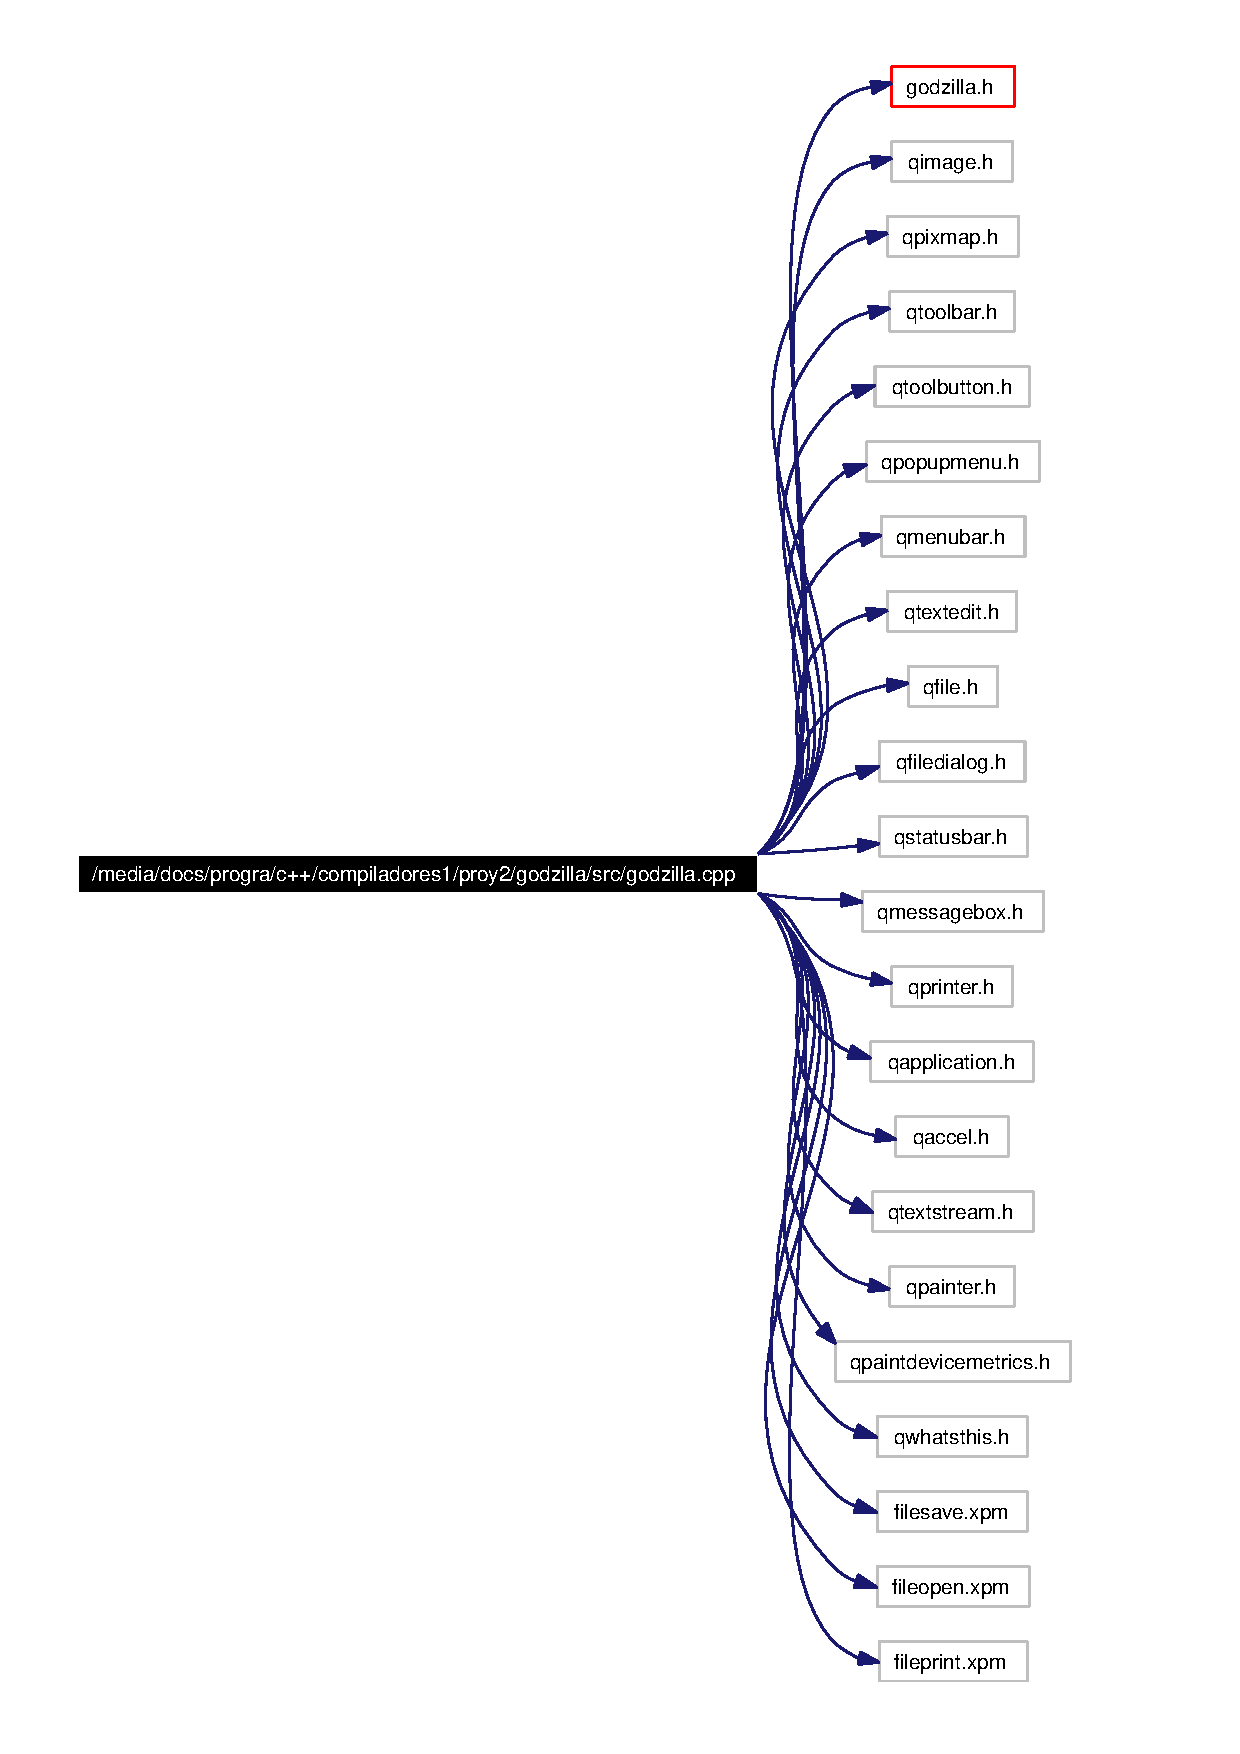
\includegraphics[width=257pt]{godzilla_8cpp__incl}
\end{center}
\end{figure}


\subsection{Descripci\'{o}n detallada}
Implementacion de la Widged principal del GUI. 



Definici\'{o}n en el archivo {\bf godzilla.cpp}.
\section{Referencia del Archivo /media/docs/progra/c++/compiladores1/proy2/godzilla/src/godzilla.h}
\label{godzilla_8h}\index{/media/docs/progra/c++/compiladores1/proy2/godzilla/src/godzilla.h@{/media/docs/progra/c++/compiladores1/proy2/godzilla/src/godzilla.h}}
defiinicion de la Widged principal del GUI. 

{\tt \#include $<$qmainwindow.h$>$}\par
{\tt \#include $<$qlabel.h$>$}\par
{\tt \#include $<$cstdlib$>$}\par
{\tt \#include $<$qtextbrowser.h$>$}\par
{\tt \#include \char`\"{}browser.h\char`\"{}}\par
{\tt \#include \char`\"{}parserheader.h\char`\"{}}\par
{\tt \#include \char`\"{}ast.h\char`\"{}}\par
{\tt \#include \char`\"{}colaerr.h\char`\"{}}\par


Dependencia gr\'{a}fica adjunta para godzilla.h:\begin{figure}[H]
\begin{center}
\leavevmode
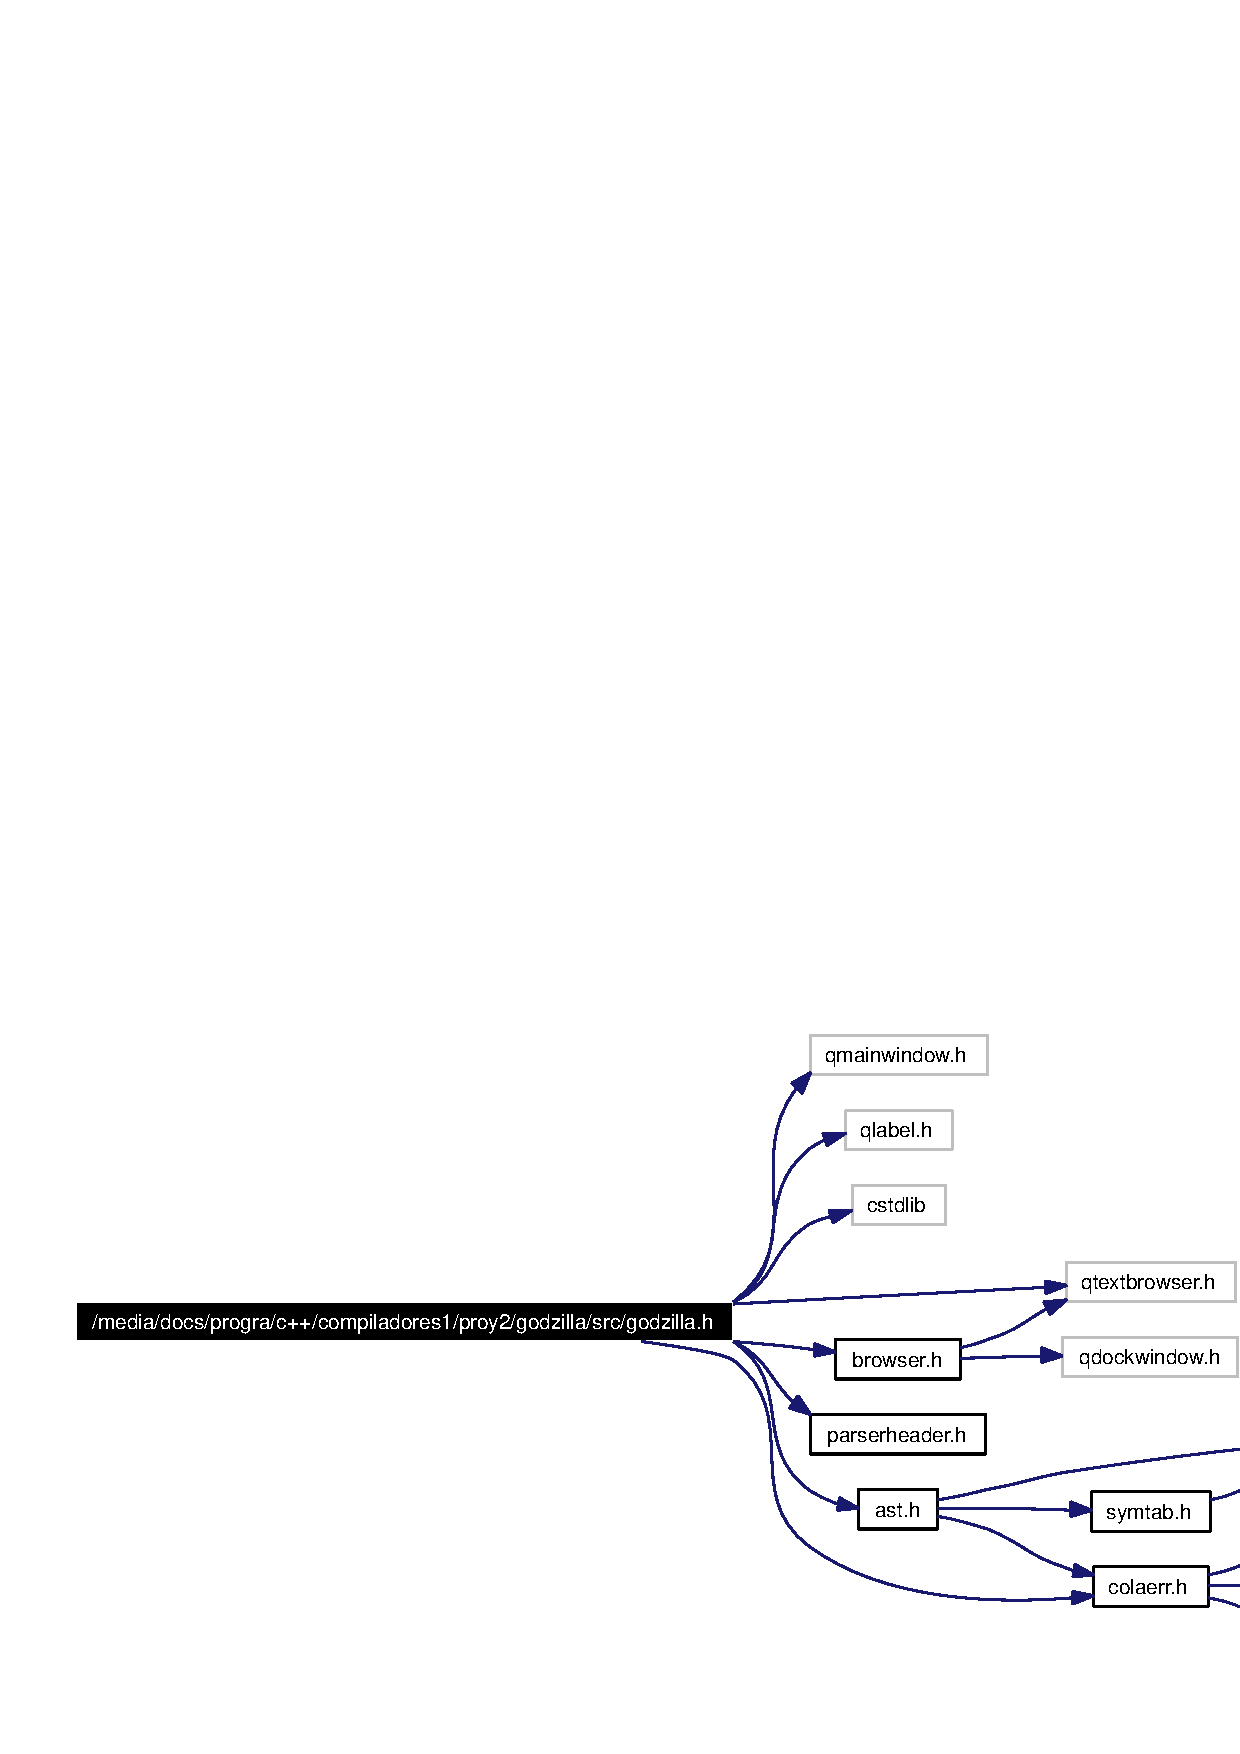
\includegraphics[width=352pt]{godzilla_8h__incl}
\end{center}
\end{figure}


Este gr\'{a}fico muestra que archivos directa o indirectamente incluyen a este archivo:\begin{figure}[H]
\begin{center}
\leavevmode
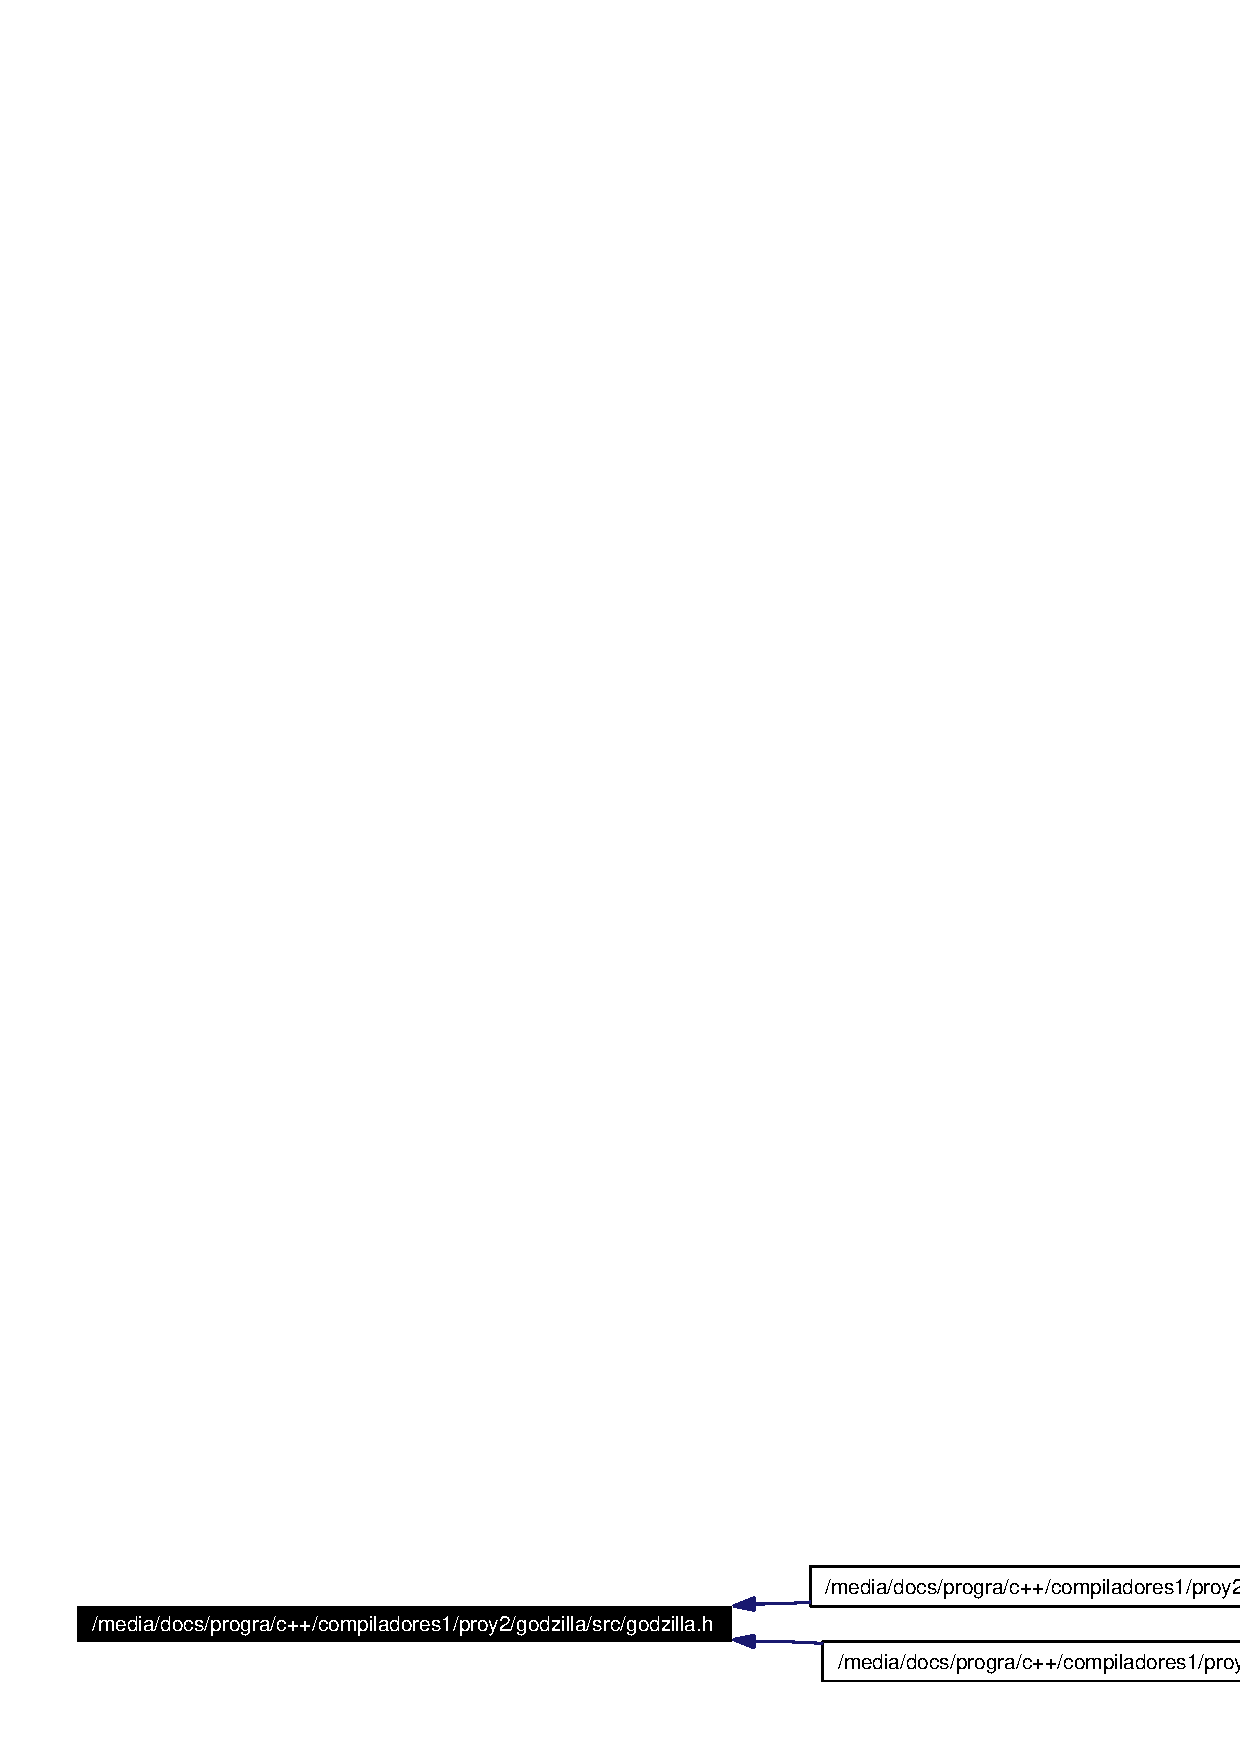
\includegraphics[width=358pt]{godzilla_8h__dep__incl}
\end{center}
\end{figure}
\subsection*{Clases}
\begin{CompactItemize}
\item 
class {\bf God\-Zilla}
\end{CompactItemize}


\subsection{Descripci\'{o}n detallada}
defiinicion de la Widged principal del GUI. 



Definici\'{o}n en el archivo {\bf godzilla.h}.
\section{Referencia del Archivo /media/docs/progra/c++/compiladores1/proy2/godzilla/src/main.cpp}
\label{main_8cpp}\index{/media/docs/progra/c++/compiladores1/proy2/godzilla/src/main.cpp@{/media/docs/progra/c++/compiladores1/proy2/godzilla/src/main.cpp}}
Punto de entrada del programa. 

{\tt \#include $<$qapplication.h$>$}\par
{\tt \#include $<$string.h$>$}\par
{\tt \#include \char`\"{}parserheader.h\char`\"{}}\par
{\tt \#include \char`\"{}godzilla.h\char`\"{}}\par


Dependencia gr\'{a}fica adjunta para main.cpp:\begin{figure}[H]
\begin{center}
\leavevmode
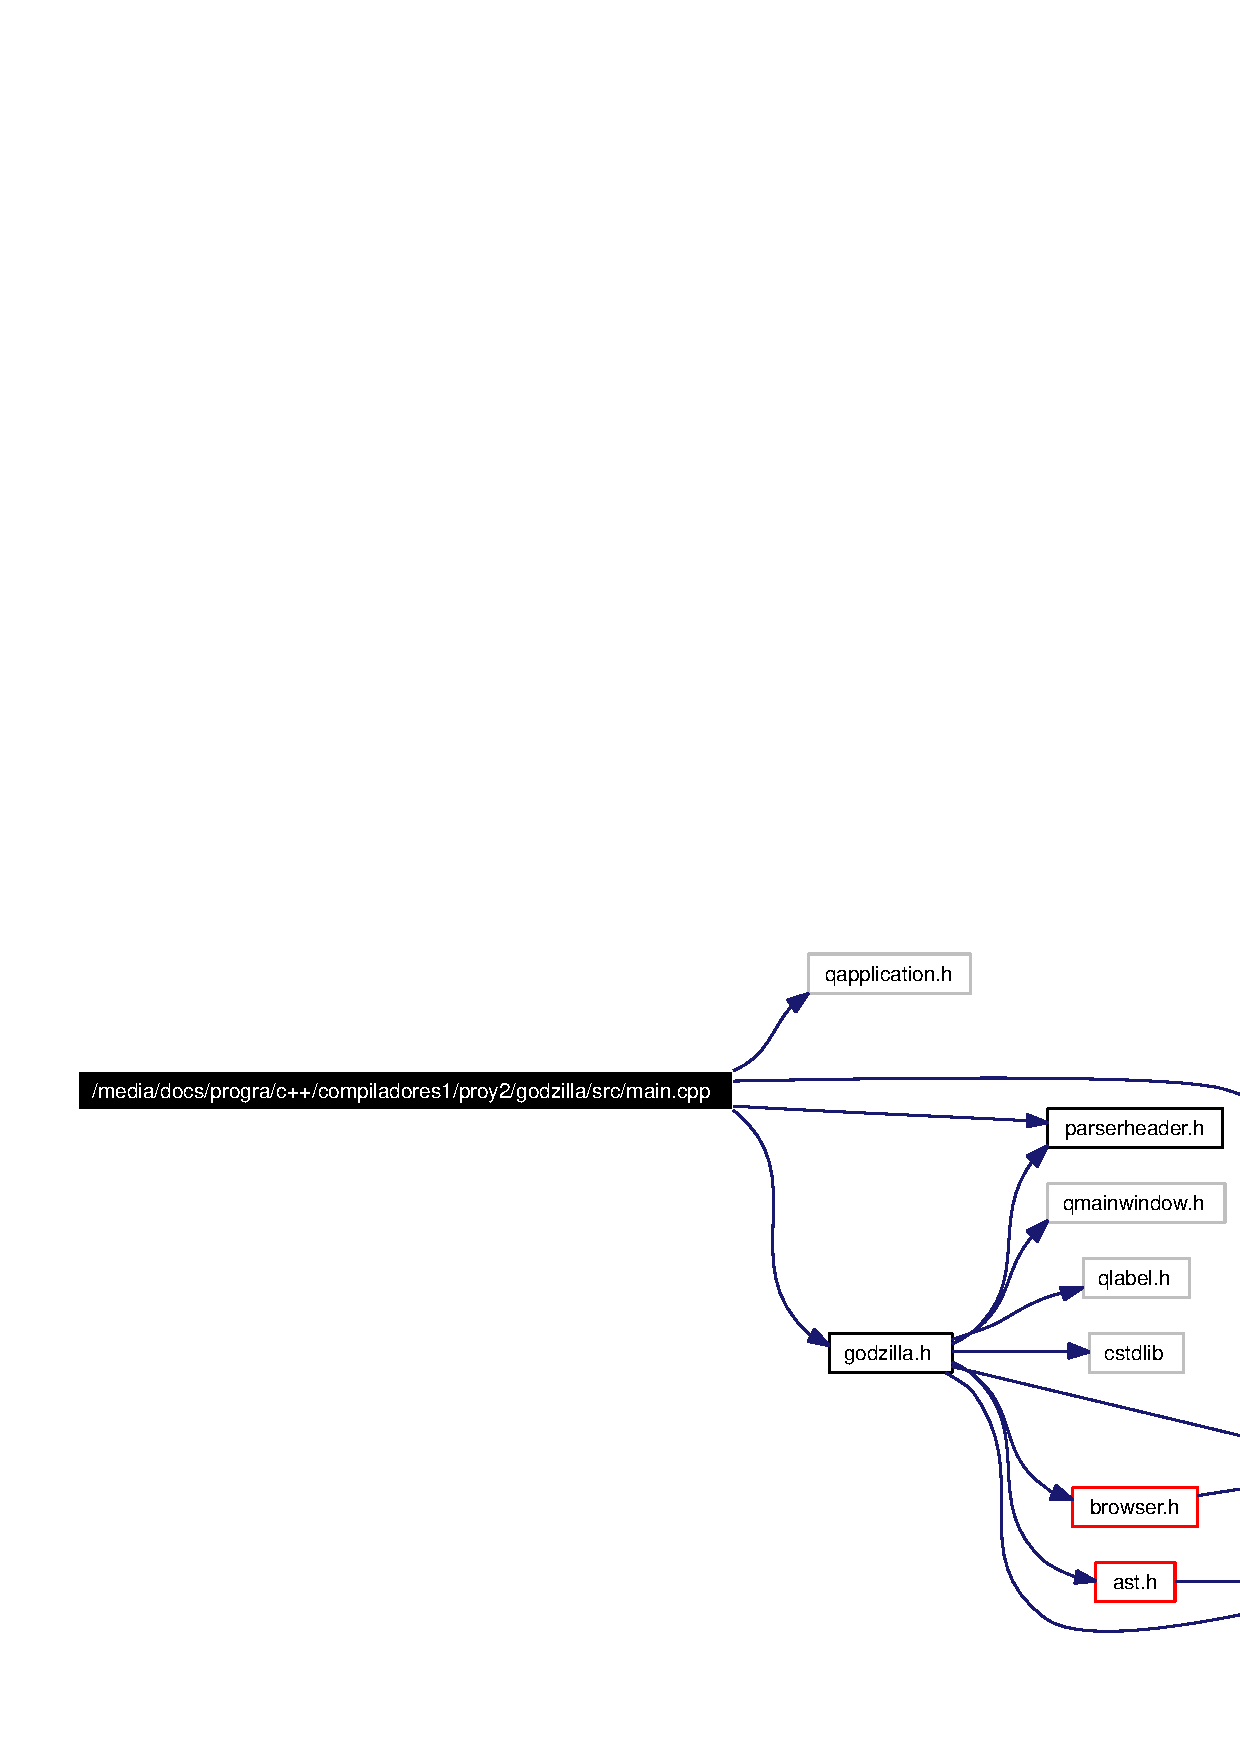
\includegraphics[width=396pt]{main_8cpp__incl}
\end{center}
\end{figure}
\subsection*{Funciones}
\begin{CompactItemize}
\item 
int {\bf main} (int argc, char $\ast$$\ast$argv)
\begin{CompactList}\small\item\em Crea objetos QApplication y {\bf God\-Zilla}{\rm (p.\,\pageref{classGodZilla})}, y los ejecuta para mostrar interfaz grafica. \item\end{CompactList}\end{CompactItemize}


\subsection{Descripci\'{o}n detallada}
Punto de entrada del programa. 



Definici\'{o}n en el archivo {\bf main.cpp}.

\subsection{Documentaci\'{o}n de las funciones}
\index{main.cpp@{main.cpp}!main@{main}}
\index{main@{main}!main.cpp@{main.cpp}}
\subsubsection{\setlength{\rightskip}{0pt plus 5cm}int main (int {\em argc}, char $\ast$$\ast$ {\em argv})}\label{main_8cpp_a0}


Crea objetos QApplication y {\bf God\-Zilla}{\rm (p.\,\pageref{classGodZilla})}, y los ejecuta para mostrar interfaz grafica. 



Definici\'{o}n en la l\'{\i}nea 16 del archivo main.cpp.

Hace referencia a generar\-Salida\-Error(), y inputparse().
\section{Referencia del Archivo /media/docs/progra/c++/compiladores1/proy2/godzilla/src/parserheader.h}
\label{parserheader_8h}\index{/media/docs/progra/c++/compiladores1/proy2/godzilla/src/parserheader.h@{/media/docs/progra/c++/compiladores1/proy2/godzilla/src/parserheader.h}}
interfaz entre el GUI y el parser. 



Este gr\'{a}fico muestra que archivos directa o indirectamente incluyen a este archivo:\begin{figure}[H]
\begin{center}
\leavevmode
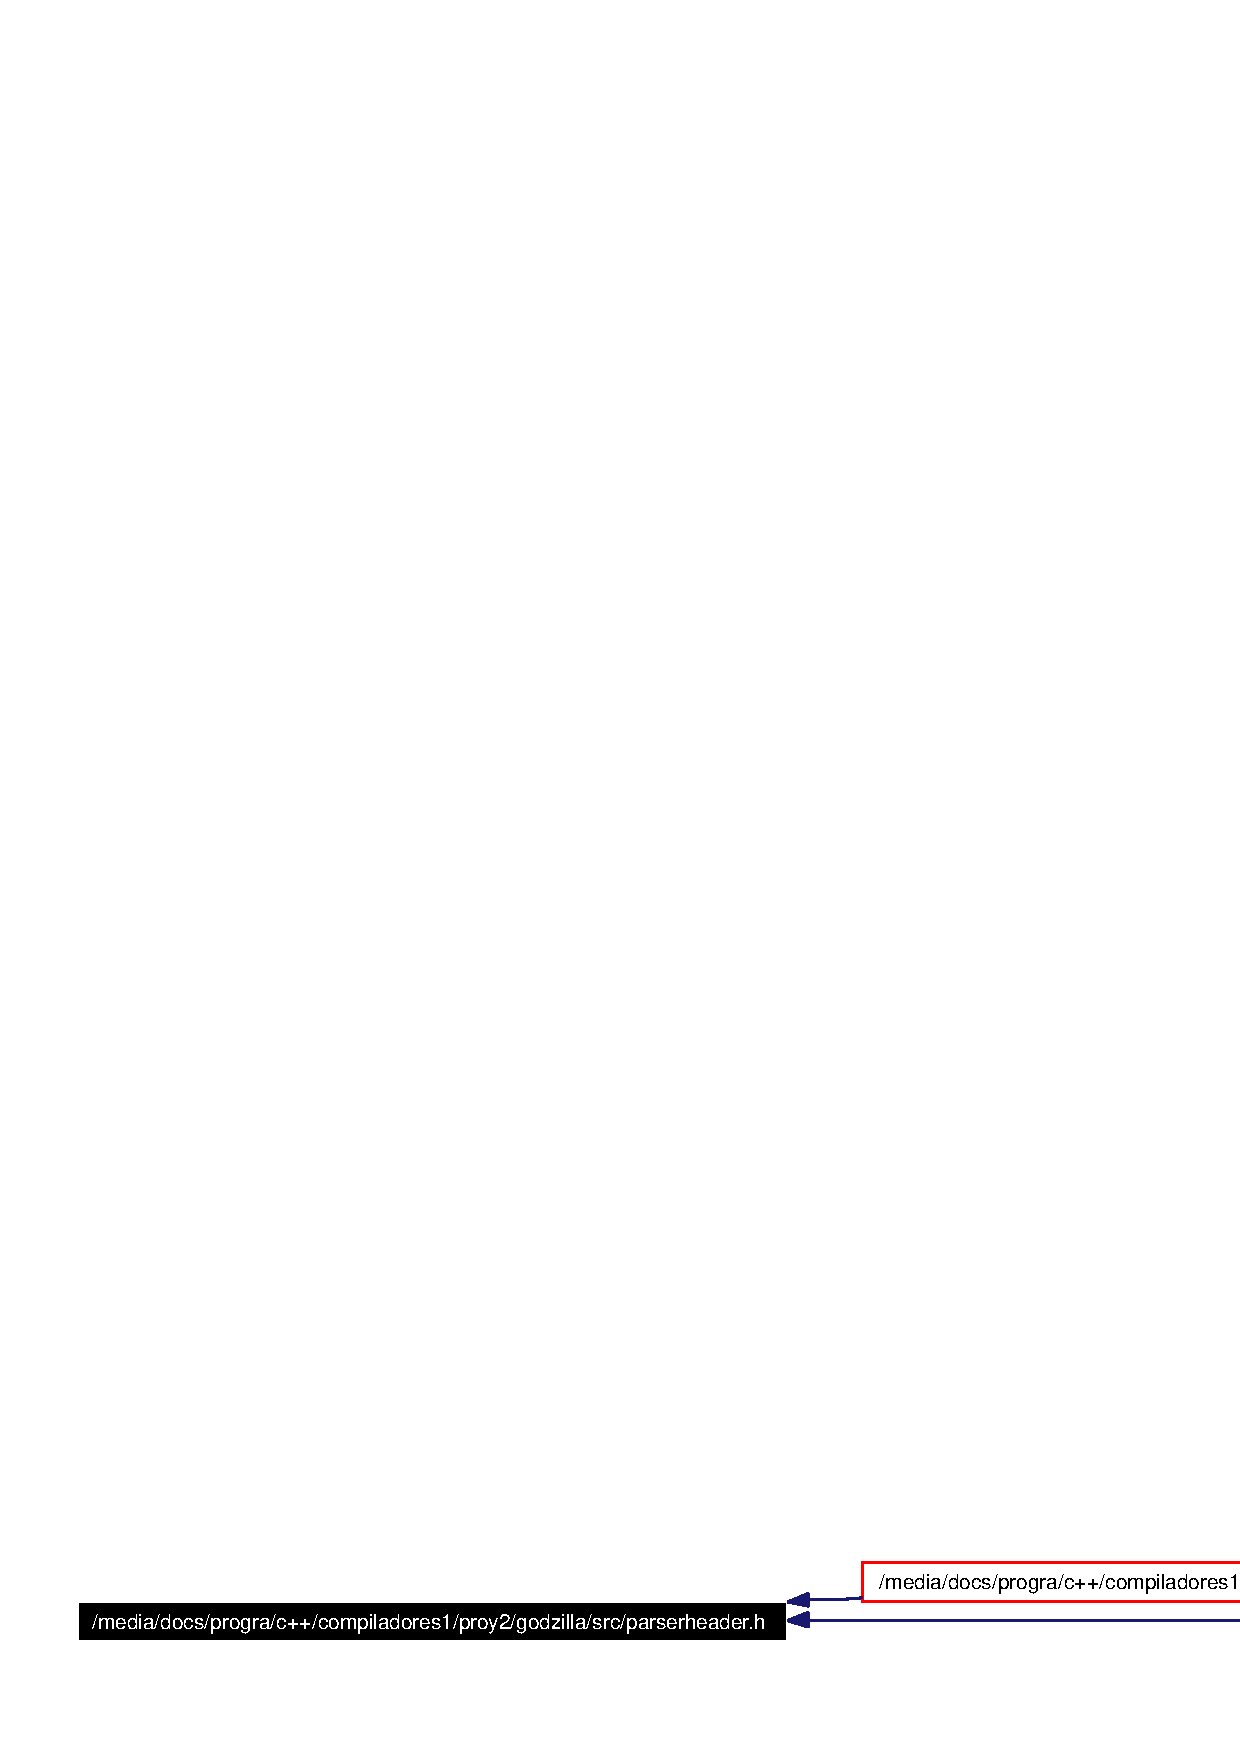
\includegraphics[width=420pt]{parserheader_8h__dep__incl}
\end{center}
\end{figure}
\subsection*{Funciones}
\begin{CompactItemize}
\item 
int {\bf inputparse} (const char $\ast$filein, const char $\ast$fileout)
\begin{CompactList}\small\item\em Interfaz para parser y lexer. \item\end{CompactList}\item 
int {\bf generar\-Salida\-Error} (const char $\ast$fileerr)
\begin{CompactList}\small\item\em Interfaz para colaerr. \item\end{CompactList}\end{CompactItemize}


\subsection{Descripci\'{o}n detallada}
interfaz entre el GUI y el parser. 



Definici\'{o}n en el archivo {\bf parserheader.h}.

\subsection{Documentaci\'{o}n de las funciones}
\index{parserheader.h@{parserheader.h}!generarSalidaError@{generarSalidaError}}
\index{generarSalidaError@{generarSalidaError}!parserheader.h@{parserheader.h}}
\subsubsection{\setlength{\rightskip}{0pt plus 5cm}int generar\-Salida\-Error (const char $\ast$ {\em fileerr})}\label{parserheader_8h_a1}


Interfaz para colaerr. 



Referenciado por main(), y God\-Zilla::parse\-Input().\index{parserheader.h@{parserheader.h}!inputparse@{inputparse}}
\index{inputparse@{inputparse}!parserheader.h@{parserheader.h}}
\subsubsection{\setlength{\rightskip}{0pt plus 5cm}int inputparse (const char $\ast$ {\em filein}, const char $\ast$ {\em fileout})}\label{parserheader_8h_a0}


Interfaz para parser y lexer. 



Referenciado por main(), y God\-Zilla::parse\-Input().
\section{Referencia del Archivo /media/docs/progra/c++/compiladores1/proy2/godzilla/src/symtab.c}
\label{symtab_8c}\index{/media/docs/progra/c++/compiladores1/proy2/godzilla/src/symtab.c@{/media/docs/progra/c++/compiladores1/proy2/godzilla/src/symtab.c}}
Implementacion de la tabla de simbolos.Incluye la implementacion de rutinas de insercion, busqueda y eliminacion. 

{\tt \#include $<$stdio.h$>$}\par
{\tt \#include $<$stdlib.h$>$}\par
{\tt \#include $<$string.h$>$}\par
{\tt \#include \char`\"{}symtab.h\char`\"{}}\par
{\tt \#include \char`\"{}constantes.h\char`\"{}}\par


Dependencia gr\'{a}fica adjunta para symtab.c:\begin{figure}[H]
\begin{center}
\leavevmode
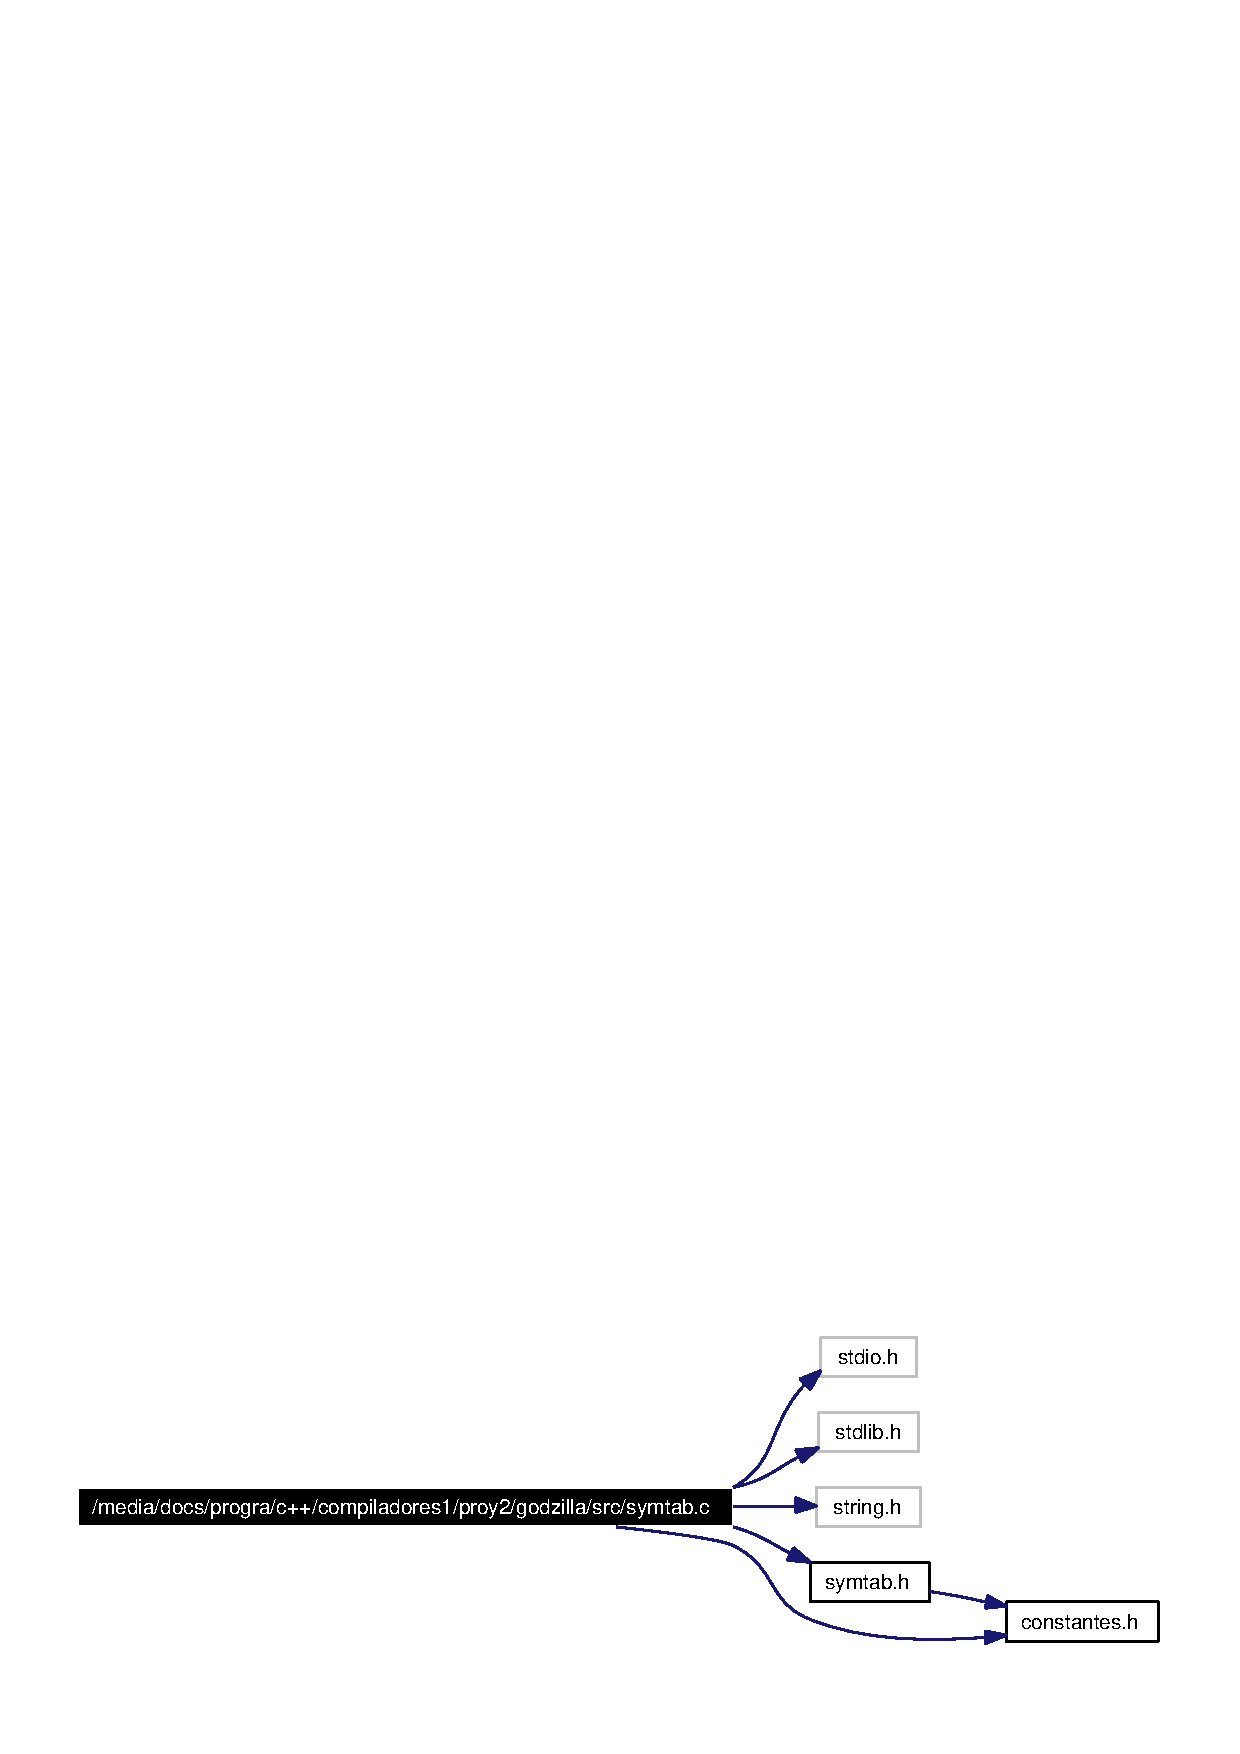
\includegraphics[width=278pt]{symtab_8c__incl}
\end{center}
\end{figure}
\subsection*{Funciones}
\begin{CompactItemize}
\item 
{\bf symbol} $\ast$ {\bf insertar\-Simbolo} (char $\ast$id, int tipo)
\begin{CompactList}\small\item\em Inserta un nuevo simbolo sin comprobar su previa existencia. \item\end{CompactList}\item 
{\bf symbol} $\ast$ {\bf buscar\-Simbolo} (char $\ast$id)
\begin{CompactList}\small\item\em Busca y devuelve simbolo segun su identificador dado en el param. \item\end{CompactList}\item 
void {\bf borrar\-Nodos} ({\bf symbol} $\ast$s)
\item 
void {\bf borrar\-Tabla} ()
\begin{CompactList}\small\item\em Elimina todos los registros de la tabla de simbolos. \item\end{CompactList}\item 
int {\bf open\-Symtab\-File} (const char $\ast$filename)
\begin{CompactList}\small\item\em Abre archivo hacia donde se imprimira archivo de tabla de simbolos. \item\end{CompactList}\item 
int {\bf close\-Symtab\-File} ()
\begin{CompactList}\small\item\em Cierra archivo hacia donde se escribio tabla de simbolos. \item\end{CompactList}\item 
int {\bf print\-Symtab\-File} (int linea)
\begin{CompactList}\small\item\em Imprime tabla de simbolos a archivo dado. \item\end{CompactList}\end{CompactItemize}
\subsection*{Variables}
\begin{CompactItemize}
\item 
static {\bf symtab} {\bf tabla}
\item 
static FILE $\ast$ {\bf symtabfile} = NULL
\begin{CompactList}\small\item\em Tabla de simbolos. \item\end{CompactList}\end{CompactItemize}


\subsection{Descripci\'{o}n detallada}
Implementacion de la tabla de simbolos.Incluye la implementacion de rutinas de insercion, busqueda y eliminacion. 



Definici\'{o}n en el archivo {\bf symtab.c}.

\subsection{Documentaci\'{o}n de las funciones}
\index{symtab.c@{symtab.c}!borrarNodos@{borrarNodos}}
\index{borrarNodos@{borrarNodos}!symtab.c@{symtab.c}}
\subsubsection{\setlength{\rightskip}{0pt plus 5cm}void borrar\-Nodos ({\bf symbol} $\ast$ {\em s})}\label{symtab_8c_a4}


No usar free() da error SIGABRT 

Definici\'{o}n en la l\'{\i}nea 74 del archivo symtab.c.

Hace referencia a symbol::id, symbol::siguiente, T\_\-STRING, symbol::tipo, y symbol::valor.

Referenciado por borrar\-Tabla().\index{symtab.c@{symtab.c}!borrarTabla@{borrarTabla}}
\index{borrarTabla@{borrarTabla}!symtab.c@{symtab.c}}
\subsubsection{\setlength{\rightskip}{0pt plus 5cm}void borrar\-Tabla (void)}\label{symtab_8c_a5}


Elimina todos los registros de la tabla de simbolos. 



Definici\'{o}n en la l\'{\i}nea 88 del archivo symtab.c.

Hace referencia a symtab::actual, borrar\-Nodos(), y symtab::primero.\index{symtab.c@{symtab.c}!buscarSimbolo@{buscarSimbolo}}
\index{buscarSimbolo@{buscarSimbolo}!symtab.c@{symtab.c}}
\subsubsection{\setlength{\rightskip}{0pt plus 5cm}{\bf symbol}$\ast$ buscar\-Simbolo (char $\ast$ {\em id})}\label{symtab_8c_a3}


Busca y devuelve simbolo segun su identificador dado en el param. 

\begin{Desc}
\item[Par\'{a}metros:]
\begin{description}
\item[{\em id}]identificador de la variable a buscar \end{description}
\end{Desc}


Definici\'{o}n en la l\'{\i}nea 60 del archivo symtab.c.

Hace referencia a symtab::actual, symtab::primero, y symbol::siguiente.

Referenciado por evaluar\-Asignacion(), evaluar\-Declaracion(), evaluar\-Expresion(), evaluar\-For(), y imprimir\-Tokens().\index{symtab.c@{symtab.c}!closeSymtabFile@{closeSymtabFile}}
\index{closeSymtabFile@{closeSymtabFile}!symtab.c@{symtab.c}}
\subsubsection{\setlength{\rightskip}{0pt plus 5cm}int close\-Symtab\-File (void)}\label{symtab_8c_a7}


Cierra archivo hacia donde se escribio tabla de simbolos. 



Definici\'{o}n en la l\'{\i}nea 113 del archivo symtab.c.

Hace referencia a symtabfile.\index{symtab.c@{symtab.c}!insertarSimbolo@{insertarSimbolo}}
\index{insertarSimbolo@{insertarSimbolo}!symtab.c@{symtab.c}}
\subsubsection{\setlength{\rightskip}{0pt plus 5cm}{\bf symbol}$\ast$ insertar\-Simbolo (char $\ast$ {\em id}, int {\em tipo})}\label{symtab_8c_a2}


Inserta un nuevo simbolo sin comprobar su previa existencia. 

\begin{Desc}
\item[Par\'{a}metros:]
\begin{description}
\item[{\em id}]identificador de la nueva var. \item[{\em tipo}]tipo de datos de la var. \end{description}
\end{Desc}


Definici\'{o}n en la l\'{\i}nea 23 del archivo symtab.c.

Hace referencia a symtab::actual, symbol::id, symtab::primero, symbol::siguiente, T\_\-BOOLEAN, T\_\-INTEGER, T\_\-STRING, symbol::tipo, y symbol::valor.

Referenciado por evaluar\-Declaracion().\index{symtab.c@{symtab.c}!openSymtabFile@{openSymtabFile}}
\index{openSymtabFile@{openSymtabFile}!symtab.c@{symtab.c}}
\subsubsection{\setlength{\rightskip}{0pt plus 5cm}int open\-Symtab\-File (const char $\ast$ {\em filename})}\label{symtab_8c_a6}


Abre archivo hacia donde se imprimira archivo de tabla de simbolos. 

\begin{Desc}
\item[Par\'{a}metros:]
\begin{description}
\item[{\em filename}]nombre de archivo al que se le adjuntara la extension xml\end{description}
\end{Desc}
trunca a cero el archivo xml 

Definici\'{o}n en la l\'{\i}nea 99 del archivo symtab.c.

Hace referencia a symtabfile.\index{symtab.c@{symtab.c}!printSymtabFile@{printSymtabFile}}
\index{printSymtabFile@{printSymtabFile}!symtab.c@{symtab.c}}
\subsubsection{\setlength{\rightskip}{0pt plus 5cm}int print\-Symtab\-File (int {\em linea})}\label{symtab_8c_a8}


Imprime tabla de simbolos a archivo dado. 

\begin{Desc}
\item[Par\'{a}metros:]
\begin{description}
\item[{\em linea}]linea en donde se leyo el comando vertablasimbolos() \end{description}
\end{Desc}


Definici\'{o}n en la l\'{\i}nea 122 del archivo symtab.c.

Hace referencia a symtab::actual, symbol::id, symtab::primero, symbol::siguiente, symtabfile, T\_\-BOOLEAN, T\_\-INTEGER, T\_\-STRING, symbol::tipo, y symbol::valor.

Referenciado por insertar\-Llamada\-Sym\-Tab().

\subsection{Documentaci\'{o}n de las variables}
\index{symtab.c@{symtab.c}!symtabfile@{symtabfile}}
\index{symtabfile@{symtabfile}!symtab.c@{symtab.c}}
\subsubsection{\setlength{\rightskip}{0pt plus 5cm}FILE$\ast$ {\bf symtabfile} = NULL\hspace{0.3cm}{\tt  [static]}}\label{symtab_8c_a1}


Tabla de simbolos. 



Definici\'{o}n en la l\'{\i}nea 20 del archivo symtab.c.

Referenciado por close\-Symtab\-File(), open\-Symtab\-File(), y print\-Symtab\-File().\index{symtab.c@{symtab.c}!tabla@{tabla}}
\index{tabla@{tabla}!symtab.c@{symtab.c}}
\subsubsection{\setlength{\rightskip}{0pt plus 5cm}{\bf symtab} {\bf tabla}\hspace{0.3cm}{\tt  [static]}}\label{symtab_8c_a0}




Definici\'{o}n en la l\'{\i}nea 19 del archivo symtab.c.
\section{Referencia del Archivo /media/docs/progra/c++/compiladores1/proy2/godzilla/src/symtab.h}
\label{symtab_8h}\index{/media/docs/progra/c++/compiladores1/proy2/godzilla/src/symtab.h@{/media/docs/progra/c++/compiladores1/proy2/godzilla/src/symtab.h}}
Estructuras de la tabla de simbolos.Incluyendo rutinas de insercion, busqueda y eliminacion. 

{\tt \#include \char`\"{}constantes.h\char`\"{}}\par


Dependencia gr\'{a}fica adjunta para symtab.h:\begin{figure}[H]
\begin{center}
\leavevmode
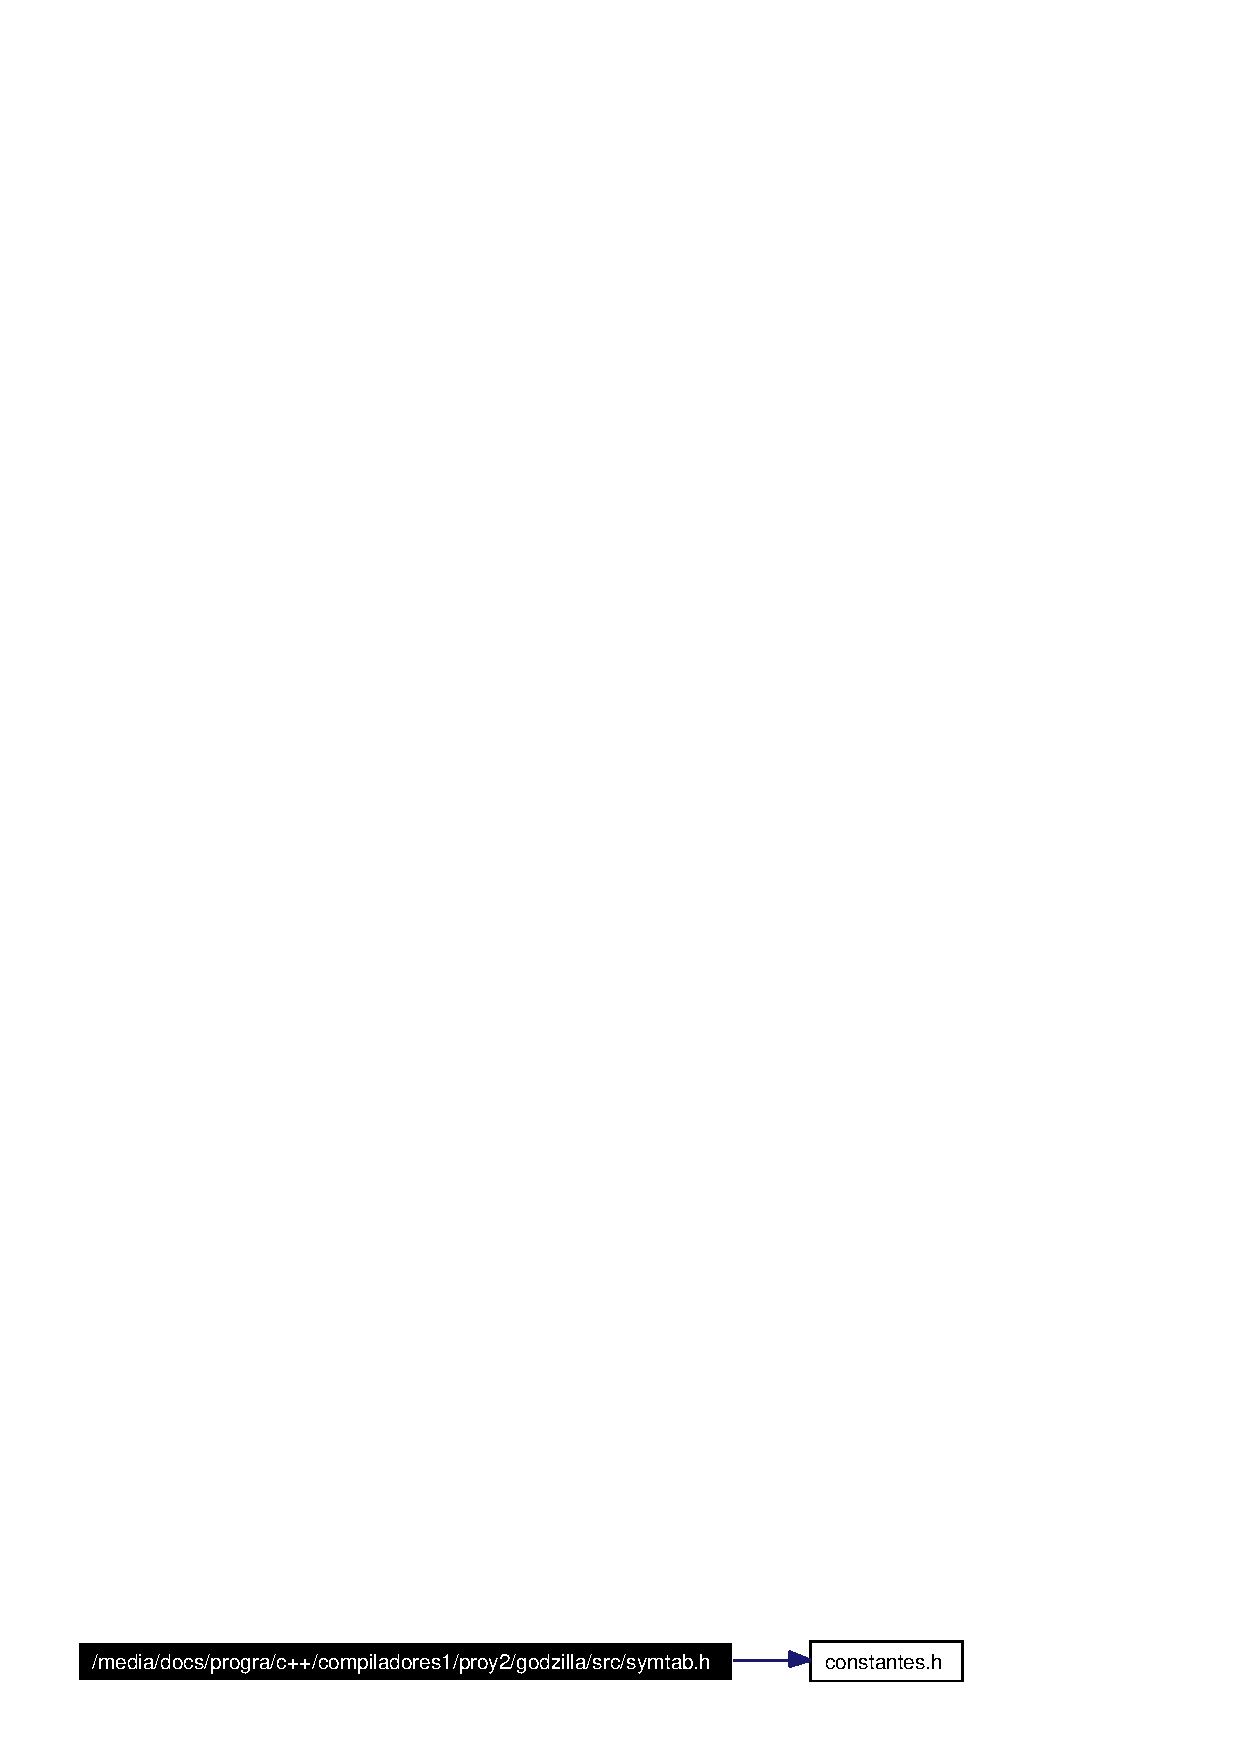
\includegraphics[width=231pt]{symtab_8h__incl}
\end{center}
\end{figure}


Este gr\'{a}fico muestra que archivos directa o indirectamente incluyen a este archivo:\begin{figure}[H]
\begin{center}
\leavevmode
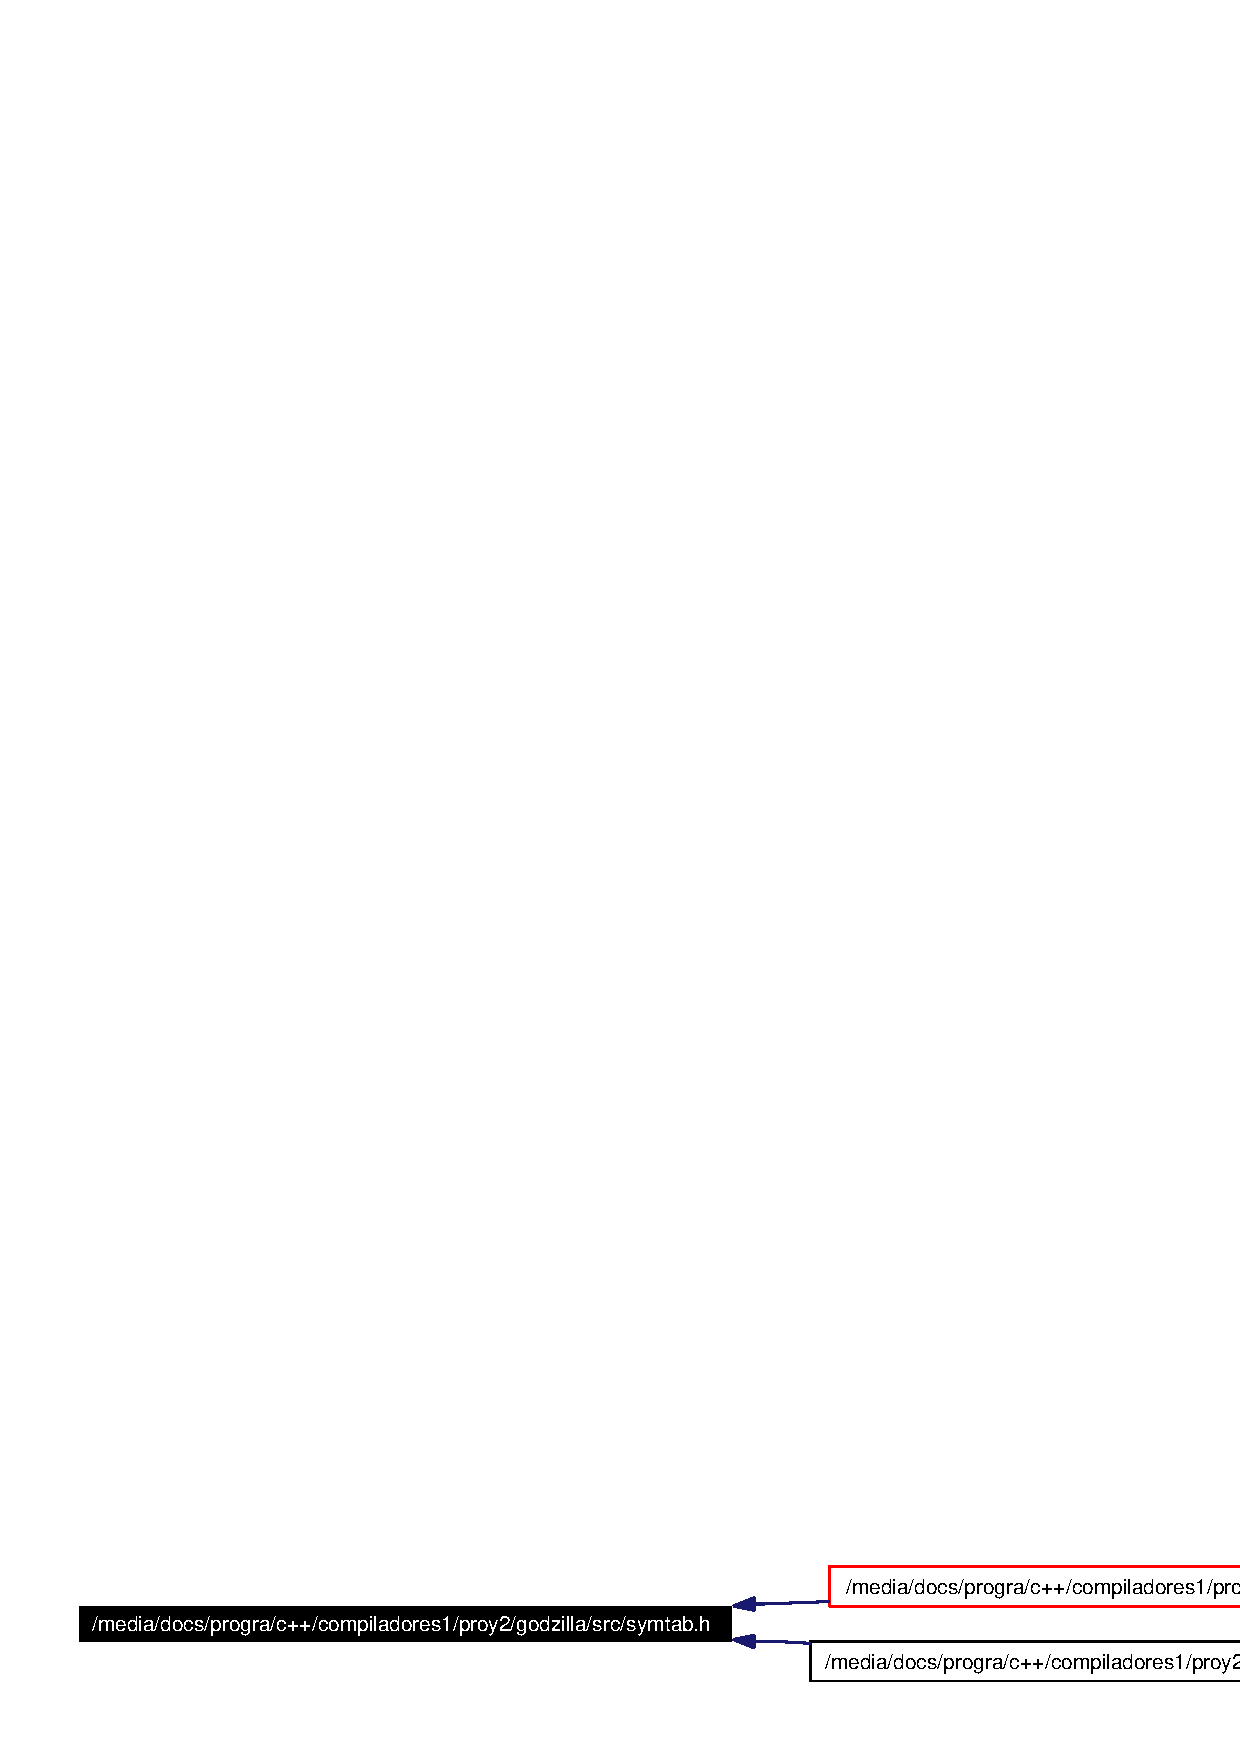
\includegraphics[width=352pt]{symtab_8h__dep__incl}
\end{center}
\end{figure}
\subsection*{Clases}
\begin{CompactItemize}
\item 
struct {\bf symbol}
\begin{CompactList}\small\item\em Nodo de la tabla de simbolos. \item\end{CompactList}\item 
struct {\bf symtab}
\begin{CompactList}\small\item\em Tabla de simbolos usando modelo de lista simple. \item\end{CompactList}\end{CompactItemize}
\subsection*{Tipos definidos}
\begin{CompactItemize}
\item 
typedef {\bf symtab} {\bf symtab}
\begin{CompactList}\small\item\em ESTRUCTURA. \item\end{CompactList}\item 
typedef {\bf symbol} {\bf symbol}
\end{CompactItemize}
\subsection*{Funciones}
\begin{CompactItemize}
\item 
{\bf symbol} $\ast$ {\bf insertar\-Simbolo} (char $\ast$id, int tipo)
\begin{CompactList}\small\item\em Inserta un nuevo simbolo sin comprobar su previa existencia. \item\end{CompactList}\item 
{\bf symbol} $\ast$ {\bf buscar\-Simbolo} (char $\ast$id)
\begin{CompactList}\small\item\em Busca y devuelve simbolo segun su identificador dado en el param. \item\end{CompactList}\item 
void {\bf borrar\-Tabla} (void)
\begin{CompactList}\small\item\em Elimina todos los registros de la tabla de simbolos. \item\end{CompactList}\item 
int {\bf open\-Symtab\-File} (const char $\ast$filename)
\begin{CompactList}\small\item\em Abre archivo hacia donde se imprimira archivo de tabla de simbolos. \item\end{CompactList}\item 
int {\bf close\-Symtab\-File} (void)
\begin{CompactList}\small\item\em Cierra archivo hacia donde se escribio tabla de simbolos. \item\end{CompactList}\item 
int {\bf print\-Symtab\-File} (int linea)
\begin{CompactList}\small\item\em Imprime tabla de simbolos a archivo dado. \item\end{CompactList}\end{CompactItemize}


\subsection{Descripci\'{o}n detallada}
Estructuras de la tabla de simbolos.Incluyendo rutinas de insercion, busqueda y eliminacion. 



Definici\'{o}n en el archivo {\bf symtab.h}.

\subsection{Documentaci\'{o}n de los tipos definidos}
\index{symtab.h@{symtab.h}!symbol@{symbol}}
\index{symbol@{symbol}!symtab.h@{symtab.h}}
\subsubsection{\setlength{\rightskip}{0pt plus 5cm}typedef struct {\bf symbol} {\bf symbol}}\label{symtab_8h_a1}




Definici\'{o}n en la l\'{\i}nea 11 del archivo symtab.h.\index{symtab.h@{symtab.h}!symtab@{symtab}}
\index{symtab@{symtab}!symtab.h@{symtab.h}}
\subsubsection{\setlength{\rightskip}{0pt plus 5cm}typedef struct {\bf symtab} {\bf symtab}}\label{symtab_8h_a0}


ESTRUCTURA. 



Definici\'{o}n en la l\'{\i}nea 10 del archivo symtab.h.

\subsection{Documentaci\'{o}n de las funciones}
\index{symtab.h@{symtab.h}!borrarTabla@{borrarTabla}}
\index{borrarTabla@{borrarTabla}!symtab.h@{symtab.h}}
\subsubsection{\setlength{\rightskip}{0pt plus 5cm}void borrar\-Tabla (void)}\label{symtab_8h_a4}


Elimina todos los registros de la tabla de simbolos. 



Definici\'{o}n en la l\'{\i}nea 88 del archivo symtab.c.

Hace referencia a symtab::actual, borrar\-Nodos(), y symtab::primero.\index{symtab.h@{symtab.h}!buscarSimbolo@{buscarSimbolo}}
\index{buscarSimbolo@{buscarSimbolo}!symtab.h@{symtab.h}}
\subsubsection{\setlength{\rightskip}{0pt plus 5cm}{\bf symbol}$\ast$ buscar\-Simbolo (char $\ast$ {\em id})}\label{symtab_8h_a3}


Busca y devuelve simbolo segun su identificador dado en el param. 

\begin{Desc}
\item[Par\'{a}metros:]
\begin{description}
\item[{\em id}]identificador de la variable a buscar \end{description}
\end{Desc}


Definici\'{o}n en la l\'{\i}nea 60 del archivo symtab.c.

Hace referencia a symtab::actual, symtab::primero, y symbol::siguiente.

Referenciado por evaluar\-Asignacion(), evaluar\-Declaracion(), evaluar\-Expresion(), evaluar\-For(), y imprimir\-Tokens().\index{symtab.h@{symtab.h}!closeSymtabFile@{closeSymtabFile}}
\index{closeSymtabFile@{closeSymtabFile}!symtab.h@{symtab.h}}
\subsubsection{\setlength{\rightskip}{0pt plus 5cm}int close\-Symtab\-File (void)}\label{symtab_8h_a6}


Cierra archivo hacia donde se escribio tabla de simbolos. 



Definici\'{o}n en la l\'{\i}nea 113 del archivo symtab.c.

Hace referencia a symtabfile.\index{symtab.h@{symtab.h}!insertarSimbolo@{insertarSimbolo}}
\index{insertarSimbolo@{insertarSimbolo}!symtab.h@{symtab.h}}
\subsubsection{\setlength{\rightskip}{0pt plus 5cm}{\bf symbol}$\ast$ insertar\-Simbolo (char $\ast$ {\em id}, int {\em tipo})}\label{symtab_8h_a2}


Inserta un nuevo simbolo sin comprobar su previa existencia. 

\begin{Desc}
\item[Par\'{a}metros:]
\begin{description}
\item[{\em id}]identificador de la nueva var. \item[{\em tipo}]tipo de datos de la var. \end{description}
\end{Desc}


Definici\'{o}n en la l\'{\i}nea 23 del archivo symtab.c.

Hace referencia a symtab::actual, symbol::id, symtab::primero, symbol::siguiente, T\_\-BOOLEAN, T\_\-INTEGER, T\_\-STRING, symbol::tipo, y symbol::valor.

Referenciado por evaluar\-Declaracion().\index{symtab.h@{symtab.h}!openSymtabFile@{openSymtabFile}}
\index{openSymtabFile@{openSymtabFile}!symtab.h@{symtab.h}}
\subsubsection{\setlength{\rightskip}{0pt plus 5cm}int open\-Symtab\-File (const char $\ast$ {\em filename})}\label{symtab_8h_a5}


Abre archivo hacia donde se imprimira archivo de tabla de simbolos. 

\begin{Desc}
\item[Par\'{a}metros:]
\begin{description}
\item[{\em filename}]nombre de archivo al que se le adjuntara la extension xml\end{description}
\end{Desc}
trunca a cero el archivo xml 

Definici\'{o}n en la l\'{\i}nea 99 del archivo symtab.c.

Hace referencia a symtabfile.\index{symtab.h@{symtab.h}!printSymtabFile@{printSymtabFile}}
\index{printSymtabFile@{printSymtabFile}!symtab.h@{symtab.h}}
\subsubsection{\setlength{\rightskip}{0pt plus 5cm}int print\-Symtab\-File (int {\em linea})}\label{symtab_8h_a7}


Imprime tabla de simbolos a archivo dado. 

\begin{Desc}
\item[Par\'{a}metros:]
\begin{description}
\item[{\em linea}]linea en donde se leyo el comando vertablasimbolos() \end{description}
\end{Desc}


Definici\'{o}n en la l\'{\i}nea 122 del archivo symtab.c.

Hace referencia a symtab::actual, symbol::id, symtab::primero, symbol::siguiente, symtabfile, T\_\-BOOLEAN, T\_\-INTEGER, T\_\-STRING, symbol::tipo, y symbol::valor.

Referenciado por insertar\-Llamada\-Sym\-Tab().
\printindex
\end{document}
